\documentclass[a4paper,10pt]{book}
\usepackage[bottom=20mm,top=20mm,left=20mm,right=20mm]{geometry}

%-----------------------package---------------------------
\usepackage{amssymb}
\usepackage{amsthm}
\usepackage{bm}
\usepackage{booktabs}
\usepackage{braket}
\usepackage{cancel}
\usepackage{xcolor}
\usepackage{graphicx}
\usepackage{epstopdf}
\usepackage{enumerate}
\usepackage[perpage]{footmisc}
\usepackage[colorlinks=true,linkcolor=blue,citecolor=red,urlcolor=blue,linktocpage=true,breaklinks=true]{hyperref}
\usepackage{mathtools}
\usepackage{pgf}
\usepackage{subcaption}
\usepackage{times}
\usepackage{tikz}
\usepackage{titlesec}
\usepackage[colorinlistoftodos]{todonotes}
\usepackage{verbatim}
\usetikzlibrary{quantikz2}
\usetikzlibrary{3d}

%-----------------------settings---------------------------
\allowdisplaybreaks[3]
\newtheorem{theorem}{Theorem}[section]
\newtheorem{lemma}{Lemma}[section]
\newtheorem{corollary}[theorem]{Corollary}
\numberwithin{equation}{section}

%-----------------------main text---------------------------
\begin{document}
%titlepage
\begin{titlepage}
    \thispagestyle{empty}
    \vspace*{\fill}
    \begin{center}
        \LARGE{Notes on Quantum Search Algorithm}

        \vspace{30pt}
        \large{Zhongwei Jiang, Linfeng Zhao}

        \vspace{16pt}
        \large{\today}

        \vspace{20pt}
        \href{https://github.com/little-little-red/NoteForQuantumSearchAlgorithm}{Project Link: https://github.com/little-little-red/NoteForQuantumSearchAlgorithm}

        \vspace{100pt}
    \end{center}
    \vspace*{\fill}
    \newpage
\end{titlepage}
%contentspage
\pagenumbering{Roman}
\tableofcontents
\newpage
%maintext
\pagenumbering{arabic}
\chapter{Quantum Computation}

\textit{This chapter is based on the book\cite{nielsen2010}.}

\section{Quantum Gate}

\subsection{Single-qubit gate}

The number of qubits in a quantum state depends on the number of classical bits in its dimension, so we usually call a vector $\ket{\psi} = a\ket{0} + b\ket{1}$ parameterized by two complex numbers $a$ and $b$ satisfying $|a|^2 + |b|^2 = 1$ a qubit. According to the constraints and phase redundancy, the Bloch sphere representation gives us a more intuitive way to observe the qubit, an isomorphism from a qubit to the three-dimensional real sphere:
\begin{equation}\label{BlochSphereRepersentation}
    \begin{split}
        \mathbb{C}\mathbb{P}^{1}                                                                              & \to S^{2}                                                                            \\
        \ket{\psi} = \cos \frac{\theta}{2}\ket{0} + \mathrm{e}^{\mathrm{i}\varphi}\sin\frac{\theta}{2}\ket{1} & \mapsto \vec{n}_{\psi}=(\cos\varphi\sin\theta,\sin\varphi\sin\theta,\cos\theta)^{T}.
    \end{split}
\end{equation}
where $\theta\in\left[0,\pi\right]$ and $\varphi\in\left[0,2\pi\right]$.

Operations on a qubit must preserve the norm and thus are described by $2\times2$ unitary matrices. By $\det|U|=e^{2i\alpha}$ Then
\begin{equation}
    e^{-i\alpha}U\in SU(2)
\end{equation}
They're only off by one global phase, so we usually ignore the global phase and only consider $SU(2)$. The Lie group $SU(2)$ has three generators $i\sigma_j$, $\sigma_j$ called Pauli matrices:
\begin{equation}
    \sigma_x = \begin{pmatrix} 0 & 1 \\ 1 & 0 \end{pmatrix}, \quad
    \sigma_y = \begin{pmatrix} 0 & -i \\ i & 0 \end{pmatrix}, \quad
    \sigma_z = \begin{pmatrix} 1 & 0 \\ 0 & -1 \end{pmatrix}.
\end{equation}
From Lie group elements, any single-qubit unitary can be written as a product of exponentials of Pauli matrices by a global phase:
\begin{equation}
    U = e^{i\alpha}\exp\left(-i\frac{\omega}{2}\vec{n}\cdot\vec{\sigma}\right),
\end{equation}
which $\vec{n}$ is the coordinates of the rotation axis on the Bloch sphere.
From the isomorphism \ref{BlochSphereRepersentation}, we can also induce an isomorphism of operations on two spaces:
\begin{equation}
    \begin{split}
        SU(2)/\{\pm 1\}                                             & \to SO(3)
        \\
        \exp\left(-i\frac{\omega}{2}\vec{n}\cdot\vec{\sigma}\right) & \mapsto \exp\left(\omega\vec{n}\cdot\vec{J}\right)
    \end{split}
\end{equation}
which $\omega\in\left[0,\pi\right]$ and $J_{j}$ are the three generators of Lie group $SO(3)$, the former refers to single-qubit gates and the latter to transformations on the Bloch sphere. For visualization and convenience, we let $R_{\vec{n}}(\omega) \coloneqq \exp\left(-i\frac{\omega}{2}\vec{n}\cdot\vec{\sigma}\right)$.

In the following, we use $XYZ$ instead of $\sigma_x\sigma_y\sigma_z$, here are some other single-qubit gates which are frequently used, they are called Hadamard gate, phase gate, and $\pi/8$ gate:
\begin{equation}
    H = \frac{1}{\sqrt{2}}\begin{pmatrix} 1 & 1 \\ 1 & -1 \end{pmatrix}, \quad
    S = \begin{pmatrix} 1 & 0 \\ 0 & i \end{pmatrix}, \quad
    T = \begin{pmatrix} 1 & 0 \\ 0 & e^{i\pi/4} \end{pmatrix}.
\end{equation}



\subsection{Properties of single-qubit gate}

Here we list some properties of single-qubit gates:
\begin{theorem}\label{the:EulerAngle}
    A single qubit gate $U$ can be decomposed into the following form
    \begin{equation}
        U=e^{i\alpha}R_{z}(\beta)R_{y}(\gamma)R_{z}(\delta).
    \end{equation}
\end{theorem}
\begin{corollary}\label{cor:DecompositionByTwoAxis}
    For suitable parameters $\alpha$, $\beta_{k}$, $\gamma_{k}$ and nonparallel vectors $\vec{n}$ and $\vec{m}$, there is
    \begin{equation}
        U=e^{i\alpha}\prod_{j=1}^{k}R_{\vec{n}}(\beta_{j})R_{\vec{m}}(\gamma_{j}).
    \end{equation}
\end{corollary}
\begin{corollary}\label{DecToAXBXC}
    If $U$ is a single qubit gate, then there exists $A,B,C \in SU(2)$, $ABC=I$, and then there is
    \begin{equation}
        U = e^{i\alpha}AXBXC
    \end{equation}
\end{corollary}
\begin{proof}
    let
    \begin{equation*}
        A=R_{z}(\beta)R_{y}(\gamma/2),\ B=R_{y}(-\gamma/2)R_{z}(-(\gamma+\beta)/2),\ C=R_{z}((\gamma-\beta)/2)
    \end{equation*}
    then we have
    \begin{equation}
        AXBXC=R_{z}(\beta)R_{y}(\gamma)R_{z}(\delta)
    \end{equation}
    and $ABC=I$.
\end{proof}
\begin{theorem}\label{ProductOfPauli}
    We have the product of Pauli matrices,
    \begin{equation}
        \sigma_{j}\sigma_{k} = i\epsilon_{jk}^{l}\sigma_{l}+\delta_{jk}I.
    \end{equation}
\end{theorem}
\begin{corollary}\label{cor:CompositionOfRotation}
    The element of Lie group $SU(2)$ can be changed into the following form,
    \begin{equation}
        R_{\vec{n}}(\omega) \coloneqq \exp\left(-i\frac{\omega}{2}\vec{n}\cdot\vec{\sigma}\right)=\cos \left(\frac{\omega}{2}\right)I-i\sin \left(\frac{\omega}{2}\right)(\vec{n}\cdot\vec{\sigma}).
    \end{equation}
\end{corollary}
\begin{proof}
    Considering the Taylor expansion
    \begin{equation}
        \begin{split}
            \exp\left(-i\frac{\omega}{2}\vec{n}\cdot\vec{\sigma}\right)
             & = \sum_{k=0}^{\infty}\frac{1}{k!}\left(-i\frac{\omega}{2}\vec{n}\cdot\vec{\sigma}\right)^{k}                                                                                                                          \\
             & = \sum_{k=0}^{\infty}\frac{1}{(2k)!}\left(-i\frac{\omega}{2}\right)^{2k}(\vec{n}\cdot\vec{\sigma})^{2k} + \sum_{k=0}^{\infty}\frac{1}{(2k+1)!}\left(-i\frac{\omega}{2}\right)^{2k+1}(\vec{n}\cdot\vec{\sigma})^{2k+1} \\
             & = \cos \left(\frac{\omega}{2}\right)I-i\sin \left(\frac{\omega}{2}\right)(\vec{n}\cdot\vec{\sigma}),
        \end{split}
    \end{equation}
    where we have $(\vec{n}\cdot\vec{\sigma})^{2} = I$ from the theorem \ref{ProductOfPauli}.
\end{proof}
\begin{corollary}
    If a rotation through an angle $2\omega_{1}$ about an axis $\vec{n_{1}}$ is followed by a rotation through an angle $2\omega_{2}$ about an axis $\vec{n_{2}}$, then the overall rotation is through an angle $\omega_{12}$ about an axis $\vec{n_{12}}$ given by
    \begin{equation*}
        \begin{split}
            \cos\omega_{12}             & = \cos\omega_{1}\cos\omega_{2}-\sin\omega_{1}\sin\omega_{2}\vec{n_{1}}\cdot\vec{n_{2}}                                                      \\
            \sin\omega_{12}\vec{n_{12}} & = \sin\omega_{1}\cos\omega_{2}\vec{n_{2}}+\cos\omega_{1}\sin\omega_{2}\vec{n_{2}}+\sin\omega_{1}\sin\omega_{2}\vec{n_{1}}\times\vec{n_{2}}.
        \end{split}
    \end{equation*}
\end{corollary}
\begin{proof}
    We know $R_{\vec{n_{1}}}(2\omega_{1})=\cos\omega I-i\sin\omega(\vec{n_{1}}\cdot\vec{\sigma})$ and the same as index $2$, so the product of two rotations is
    \begin{equation*}
        \begin{split}
              & R_{\vec{n_{1}}}(2\omega_{1})R_{\vec{n_{2}}}(2\omega_{2})                                                                                                                                                                                       \\
            = & \cos\omega_{1}\cos\omega_{2}I-i\sin\omega_{1}\cos\omega_{2}(\vec{n_{1}}\cdot\vec{\sigma})-i\cos\omega_{1}\sin\omega_{2}(\vec{n_{2}}\cdot\vec{\sigma})-\sin\omega_{1}\sin\omega_{2}(\vec{n_{1}}\cdot\vec{\sigma})(\vec{n_{2}}\cdot\vec{\sigma}) \\
            = & \cos\omega_{12}I-i\sin\omega_{12}(\vec{n_{12}}\cdot\vec{\sigma}),
        \end{split}
    \end{equation*}
    where we have $(\vec{n_{1}}\cdot\vec{\sigma})(\vec{n_{2}}\cdot\vec{\sigma})=i(\vec{n_{1}}\times\vec{n_{2}})\cdot\vec{\sigma}+(\vec{n_{1}}\cdot\vec{n_{2}})\cdot\vec{\sigma}$ from Theorem \ref{ProductOfPauli}.
\end{proof}



\subsection{\label{CtrlGate}Controlled operation}

Analogous to the if statement of a classical circuit, we can use the controlled-NOT gate to control the target qubit with the control qubit, its matrix form and circuit are shown as follows:
\begin{equation}
    CNOT = \begin{pmatrix} I & 0 \\ 0 & X \end{pmatrix}
\end{equation}
\begin{equation}
    \begin{quantikz}[row sep=0.4cm]
        & \ctrl{1} & \\
        & \targ{} &
    \end{quantikz}
\end{equation}
CNOT gate makes the state of the target qubit be flipped when the control qubit is 1 and remains unchanged when the control qubit is 0. That is $\ket{c}\ket{t}\rightarrow\ket{c}X^{c}\ket{t}$. We will also use two deformations of CNOT gates:
\begin{equation}
    \begin{quantikz}
        & \targ{} & \ghost{H} \\
        & \ctrl{-1} & \ghost{H}
    \end{quantikz} = \begin{quantikz}[row sep=0.4cm,column sep=0.4cm]
        & \gate{H} & \ctrl{1} & \gate{H} & \\
        & \gate{H} & \targ{} & \gate{H} &
    \end{quantikz}
    \quad\text{and}\quad
    \begin{quantikz}
        & \octrl{1} & \ghost{X} \\
        & \targ{} &
    \end{quantikz} = \begin{quantikz}[row sep=0.4cm,column sep=0.4cm]
        & \gate{X} & \ctrl{1} & \gate{X} & \\
        & & \targ{} & &
    \end{quantikz}
\end{equation}

We expect to extend this control from $X$ to an arbitrary single-qubit gate $U$. That is, $\ket{c}\ket{t}\rightarrow\ket{c}U^{c}\ket{t}$ which is known as a controlled-U gate. Show that:
\begin{equation}
    \begin{quantikz}[row sep=0.4cm]
        & \ctrl{1} & \\
        & \gate{U} &
    \end{quantikz}
\end{equation}
We wish to decompose this into combining single quantum bit gates and CNOT gates. With the theorem\ref{DecToAXBXC}, we can divide the controlled-U gate into several parts, looking first at the global phase part, which has:
\begin{equation}
    \begin{quantikz}[row sep=0.4cm]
        & \ctrl{1} & \ghost{phase} \\
        & \gate{e^{i\alpha}I} &
    \end{quantikz} = \begin{quantikz}[row sep=0.4cm]
        & \gate{phase} & \\
        & \ghost{e^{i\alpha}I} &
    \end{quantikz}
\end{equation}
where $phase = \begin{pmatrix} 1 & 0 \\ 0 & e^{i\alpha} \end{pmatrix}$.

Looking at the $AXBXC$ part again, we have the expectation that if the control qubit is $\ket{0}$, then we do nothing, and adding a CNOT gate anywhere doesn't change that, so we have.
\begin{equation}
    \begin{quantikz}
        \lstick{$\ket{0}$} & & \ghost{} \\
        \lstick{} & \gate{I} &
    \end{quantikz} = \begin{quantikz}
        & & & & \ghost{} \\
        & \gate{A} & \gate{B} & \gate{C} &
    \end{quantikz} = \begin{quantikz}
        & & \ctrl{1} & & \ctrl{1} & & \ghost{} \\
        & \gate{A} & \targ{} & \gate{B} & \targ{} & \gate{C} &
    \end{quantikz}
\end{equation}
This construction also satisfies: if the control qubit is $\ket{1}$, we apply $AXBXC$ to the target qubit.

So we have that:
\begin{theorem}
    The controlled-U gate can be decomposed with CNOT gates and single-qubit gates into this form:
    \begin{equation}
        \begin{quantikz}
            & \ctrl{1} & \ghost{X} \\
            & \gate{U} &
        \end{quantikz} = \begin{quantikz}
            & & \ctrl{1} & & \ctrl{1} & \gate{phase} & \\
            & \gate{A} & \targ{} & \gate{B} & \targ{} & \gate{C} &
        \end{quantikz}
    \end{equation}
\end{theorem}

Considering the case of multiple control qubits, first look at the case of two control qubits, you can construct: if $V$ is a single qubit gate satisfying $V^2=U$, we have:
\begin{equation}
    \begin{quantikz}
        & \ctrl{1} & \ghost{} \\
        & \ctrl{1} & \ghost{} \\
        & \gate{U} & \qw
    \end{quantikz} = \begin{quantikz}[row sep=0.5cm,column sep=0.4cm]
        & \qw & \ctrl{1} & \qw & \ctrl{1} & \ctrl{2} & \ghost{} \\
        & \ctrl{1} & \targ{} & \ctrl{1} & \targ{} & \qw & \ghost{} \\
        & \gate{V} & \qw & \gate{V^\dagger} & \qw & \gate{V} & \qw
    \end{quantikz}
\end{equation}

Then we can extend this to the case of $n$ control qubits, there are many kinds of construction methods, and we use the recursive method to construct:
\begin{equation}
    \begin{quantikz}[row sep=0.3cm]
        & \ctrl{1} & \ghost{} \\
        & \ctrl{1} & \ghost{} \\
        & \ctrl{1} & \ghost{} \\
        & \gate{U} & \qw
    \end{quantikz} = \begin{quantikz}[row sep=0.3cm,column sep=0.4cm]
        & \qw & \ctrl{1} & \qw & \ctrl{1} & \ctrl{2} & \ghost{} \\
        & \qw & \ctrl{1} & \qw & \ctrl{1} & \ctrl{2} & \ghost{} \\
        & \ctrl{1} & \targ{} & \ctrl{1} & \targ{} & \qw & \ghost{} \\
        & \gate{V} & \qw & \gate{V^\dagger} & \qw & \gate{V} & \qw
    \end{quantikz}
\end{equation}

Ultimately we will show that any unitary operation can be composed to an arbitrarily good approximation from just H, S, T, CNOT gates. Here is the construction of the Toffoli Gate:
\begin{equation}
    \begin{quantikz}[row sep=0.4cm]
        & \ctrl{1} & \ghost{} \\
        & \ctrl{1} & \ghost{} \\
        & \targ{} & \qw
    \end{quantikz} = \begin{quantikz}[row sep=0.15cm,column sep=0.25cm]
        & & & & \ctrl{2} & & & & \ctrl{2} & & \ctrl{1} & & \ctrl{1} & \gate{T} & \\
        & & \ctrl{1} & & & & \ctrl{1} & & & \gate{T^\dagger} & \targ{} & \gate{T^\dagger} & \targ{} & \gate{S} & \\
        & \gate{H} & \targ{}  & \gate{T^\dagger} & \targ{} & \gate{T} & \targ{} & \gate{T^\dagger} & \targ{} & \gate{T} & \gate{H} & & & &
    \end{quantikz}
\end{equation}



\section{Universal Gate Set}

\subsection{\label{subsec:SingleAndCnot}Single-qubit and CNOT gates are universal}

In the section \ref{CtrlGate}, we showed that $C^{n}(U)$ gate can be decomposed into a combination of single-qubit gates and CNOT gates. In this section \ref{subsec:SingleAndCnot}, we will show that any unitary gate can be combined from $C^{n}(U)$ gate.

First, we introduce the lemma:
\begin{lemma}
    Any D-dimensional unitary transformation U can always be decomposed into the product of $d(d-1)/2$ two-level unitary transformations under a natural basis.
\end{lemma}
So exists two-level unitary transformations $ V_{j} $ made $U = \prod\limits_{j=1}^{d(d-1)/2}V_{j}$\footnote{Unless otherwise specified, the conjunction sign in this document is calculated according to the composite order of the map, that is $\prod\limits_{j=1}^{n}a_{j} = a_{n}a_{n-1}\cdots a_{1}$. }. Two-level unitary transformations are unitary matrices that act non-trivially only on two or fewer vector components. The proof idea of this theorem is simple \footnote{Each single-qubit gates has $d(d-1)/2$ degrees of freedom and each two-level unitary transformation turn one of single-qubit gate elements into zero in order. So exists two-level unitary transformations $ V_{j} $ made $\left( \prod\limits_{j=1}^{d(d-1)/2}V_{j} \right) U = I $. },  let's focus on the two-level unitary transformations $V$.

Consider the binary expansion of the two bases $\ket{s}$ and $\ket{t}$ on which $V$ operates, where $s=s_{1}\ldots s_{n}$ and $t=t_{1}\ldots t_{n}$. We can use Toffoli gate to turn $s_{j}$ into $t_{j}$, after $n-1$ steps $\ket{s_{1}\ldots s_{k-1} s_{k} s_{k+1} \ldots s_{n}}$ into $\ket{t_{1}\ldots t_{k-1} s_{k} t_{k+1} \ldots t_{n}}$. It puts $\ket{s}$ and $\ket{t}$in the same qubit and makes $V$ into a $C^{n}(\widetilde{V})$ gate which $\widetilde{V}$ is the non-trivial $2\times 2$ unitary sub-matrix of $V$.

Let's take an example to illustrate this lemma, consider the $U$ gate:
\begin{equation}
    V = \begin{pmatrix} a & 0 & 0 & c \\ 0 & 1 & 0 & 0 \\ 0 & 0 & 1 & 0 \\ b & 0 & 0 & d \end{pmatrix}
    \quad \text{and} \quad
    \widetilde{V} = \begin{pmatrix} a & c \\ b & d \end{pmatrix}
\end{equation}
Notice that $V$ acts non-trivially only on the states $\ket{00}$ and $\ket{11}$, so we can use the CNOT gate to turn $\ket{00}$ into $\ket{01}$, then we can get the $C(\widetilde{V})$ gate. Here is the circuit of $V$:
\begin{equation}
    \begin{quantikz}
        & \gate[2]{V} & \qw \\
        & & \qw
    \end{quantikz} = \begin{quantikz}
        & \octrl{1} & \gate{\widetilde{V}} & \octrl{1} & \qw \\
        & \targ{} & \ctrl{-1} & \targ{} & \qw
    \end{quantikz}
\end{equation}

So we have:
\begin{theorem}
    Any unitary gate can be combined from single-qubit gates and CNOT gates.
\end{theorem}



\subsection{Approximate universal operators with a discrete set}

It is hard to implement all single-qubit gates, so we consider approximating it with a discrete set that we can implement. We introduce the induced norm of operators to measure the degree of approximation:
\begin{equation}
    E(U,V) = \left\| U-V \right\| \coloneqq \sup\limits_{\substack{\ket{\psi} \in \mathbb{C}^{n} \\ \left\| \ket{\psi} \right\| = 1}} \left\| (U-V)\ket{\psi} \right\|
\end{equation}
$U$ is the target unitary operation we wish to implement, $V$ is the unitary operation implemented in practice, and $E(U,V)$ is the error when $V$ is implemented instead of $U$. It is natural that:
\begin{theorem}
    In the approximation of $m$ gates, the error is added at most linearly:
    \begin{equation}
        E\left(\prod\limits_{j=1}^{m}U_{j},\prod\limits_{j=1}^{m}V_{j}\right) \leq \sum_{j=1}^{m} E(U_{j},V_{j})
    \end{equation}
\end{theorem}
\begin{proof}
    Considering $\ket{\psi_{0}}$ which maximizes $\left\|\left(\prod\limits_{i=1}^{m}U_{i} -  \prod\limits_{i=1}^{m}V_{i}\right)\ket{\psi}\right\|$ and definition $\ket{\psi_{i}} = V_{i}\ket{\psi_{i-1}}$ , $\ket{\Delta_{i}} = U_{i}\ket{\psi_{i-1}} - \ket{\psi_{i}}$ , we can see that
    \begin{equation*}
        E\left(\prod_{j=1}^{m}U_{j},\prod\limits_{j=1}^{m}V_{j}\right) = \left\|\ket{\Delta_{m}} + \sum\limits_{j=1}^{m-1} \left(\prod_{k=j+1}^{m}U_{k}\right)\ket{\Delta_{j}}\right\| \leq \sum\limits_{j=1}^{m} \left\|\ket{\Delta_{j}}\right\| \leq \sum_{j=1}^{m} E(U_{j},V_{j}) \qedhere
    \end{equation*}
\end{proof}


We are more concerned with the error of the approximation in the measurement. Considering $M$ is a POVM element in an arbitrary measurement POVM, and $P_{U}$(or $P_{V}$) is the probability of obtaining this outcome if $U$(or $V$) were performed with the state $\ket{\psi}$, We can prove\footnote{Let $\ket{\Delta} = (U-V)\ket{\psi}$, notice that $\bra{\psi}U^{\dagger}MU\ket{\psi} - \bra{\psi}V^{\dagger}MV\ket{\psi} = \bra{\psi}U^{\dagger}M\ket{\Delta} + \bra{\Delta}MV\ket{\psi}$. } that:
\begin{equation}
    \left| P_{U} - P_{V} \right| \leq 2E(U,V)
\end{equation}
This makes it possible that if we want the probability difference between the approximate line and the ideal line on a certain outcome to be within a tolerance $\Delta > 0$, we only need to ensure that $E(U_{j},V_{j}) \leq \Delta/(2m)$.

From the decomposition given by corollary \ref{cor:DecompositionByTwoAxis}, we can further care about the degree of approximation of $R_{\vec{n}}(\omega)$. Let's start by introducing a neat lemma :
\begin{lemma}\label{AngleCoverR}
    Considering $\alpha$, $\omega \in \mathbb{R} /2\pi\mathbb{Z}$, if $\omega/\pi \in \mathbb{R} \backslash \mathbb{Q}$ , we can find a sub-sequences $\{x_n\}$ of sequences $\{n\}$ makes $\lim\limits_{n\to\infty}x_n\omega = \alpha$.
\end{lemma}
\begin{proof}
    $\forall \epsilon>0$, $\exists N=\frac{2\pi}{\epsilon}$, when $n>N$, we can find $|j\omega-k\omega|\leq\frac{2\pi}{n}$ which $j,k \in \{n\},j>k$, let $x_{n} = (j-k)\left\lfloor\frac{\alpha}{|j\omega-k\omega|}\right\rfloor$, so we have $|x_{n}\omega-\alpha|<|j\omega-k\omega|\leq\frac{2\pi}{n}<\epsilon$.
\end{proof}
Further, we have\footnote{The construction of $x_{n}$ in this part is only to prove the existence, without considering the complexity. There are far less complex constructs.}:
\begin{equation}
    \begin{split}
          & \ E(R_{\vec{n}}(\alpha),R_{\vec{n}}(\omega)^{x_{n}})              \\
        = & \ E(R_{\vec{n}}(\alpha),R_{\vec{n}}(\alpha+(x_{n}\omega-\alpha))) \\
        = & \ |1-\exp((x_{n}\omega-\alpha)/2)|\leq\ \epsilon/2
    \end{split}
\end{equation}
According to the proof, we must find the gate with the angle the theorem requires. Fortunately, the $THTH$ gate has the angel we need. It is a rotation of the Bloch sphere about an axis along $\vec{n} = (\cos\frac{\pi}{8},\sin\frac{\pi}{8},\cos\frac{\pi}{8})$ and through an angle $\omega$ defined by $\cos\frac{\omega}{2} = \cos^{2}\frac{\pi}{8}$, so we just let $R_{\vec{n}}(\omega) = THTH$.

From corollary \ref{cor:DecompositionByTwoAxis}, to construct unitary operation $U$, we still need to approximate the rotation of the other axis, but even more fortunate is that $HR_{\vec{n}}(\omega)H$ is exactly what we need, has axis $\vec{m} = (\cos\frac{\pi}{8},-\sin\frac{\pi}{8},\cos\frac{\pi}{8})$ and the angle $\omega$, like $R_{\vec{n}}(\omega)$, is an irrational multiple of $\pi$. After layers and layers of preparation, let's list the final approximation with suitable positive integers $j_{n}$ to U:
\begin{equation}\label{FinalApproximation}
    E(U,\prod_{j=1}^{2k}R_{\vec{n}}(\omega)^{j_{n}}H) \leq k\epsilon
\end{equation}
\begin{theorem}
    Given any single qubit unitary operation $U$ and any $\epsilon > 0$, it is possible to approximate $U$ to within $\epsilon$ \footnote{The difference between Equation \ref{FinalApproximation} and here by one coefficient can be solved by the setting of $\epsilon$ in the proof of Theorem \ref{AngleCoverR}, but it does not matter. }using a circuit composed of $H$ gates and $T$ gates alone.
\end{theorem}



\subsection{Circuit size for approximation}

It makes no sense to talk about its existence without giving its size,  so let's estimate the number of gates needed for the approximation in the previous section. For convenience of stating the theorem, we say that $S$ is an $\epsilon$-net in $W$, if every point in $W$ is within a distance $\epsilon$ of some point in $S$, where $S$, $W\in SU(2)$ and $\epsilon>0$ and the distance is $D(U,V)\coloneqq\mathrm{tr}|U-V|$. And we define $\mathcal{G}_{l}$ as the set of all words of length at most $l$.
\begin{theorem}[Solovay-Kitaev theorem]
    Let $\mathcal{G}$ be a finite set of elements in $SU(2)$ containing its own inverses, such that $\left\langle\mathcal{G}\right\rangle$ is dense in $SU(2)$. Let $\epsilon > 0$ be given. Then $\mathcal{G}_{l}$ is an $\epsilon$-net in $SU(2)$ for $l=O(\ln^{c}(1/\epsilon))$, where $c=\ln5/\ln(3/2)$.
\end{theorem}
According to the theorem, we can know that to approximate a circuit containing $m$ single-qubit unitary operations to an accuracy $\epsilon$ requires $O(m\ln^{c}(m/\epsilon))$ gates from the discrete set. The proof of this theorem is quite long, so only the main ideas are given here. Let's first introduce the lemma:
\begin{lemma}
    Let $\mathcal{G}$ be a finite set of elements in $SU(2)$ containing its own inverses, such that $\left\langle\mathcal{G}\right\rangle$ is dense in $SU(2)$. For some $\epsilon>0$ and any $k\in\mathbb{N}$, if $\mathcal{G}_{l}$ is an $\epsilon^{2}$-net for $S_{\epsilon}$, then $\mathcal{G}_{5^{k}l}$ is an $\epsilon(k)^{2}$-net for $S_{\epsilon(k)}$. where $\epsilon(k)=(C\epsilon)^{(3/2)^{k}}/C$, $\epsilon(k)^{2}<\epsilon(k+1)$ and $S_{\epsilon}\coloneqq \{U\in SU(2)|D(U,I)\leq \epsilon\}$.
\end{lemma}
\begin{proof}
    We know the element of $SU(2)$ can be written as $U=\exp(-i\vec{a}\cdot\vec{\sigma}/2)$, we write $U=u(\vec{a})$.And introduce the symbol $[U,V]_{gp}=UVU^{\dagger}V^{\dagger}$. With constant $d$, we have two conclusions:
    \begin{equation}
        D([u(\vec{a}),u(\vec{b})]_{gp},u(\vec{a}\times\vec{b}))\leq d\epsilon^{3}\quad\text{and}\quad D(u(\vec{a}),u(\vec{b}))=\left\| \vec{a}-\vec{b} \right\| + O(\epsilon^{3})
    \end{equation}
    If $U=u(\vec{x})\in S_{\epsilon^{2}}$, we can find $\vec{y}\times \vec{z}=\vec{x}$ which $u(\vec{y}),u(\vec{z})\in S_{\epsilon}$, so that we can find $u(\vec{y_{0}}),u(\vec{z_{0}})\in \mathcal{G}_{l}\cap S_{\epsilon}$ make $D(u(\vec{y_{0}}),u(\vec{y})),D(u(\vec{z_{0}}),u(\vec{z}))\leq \epsilon$. Notice that
    \begin{equation}
        \begin{split}
            D(U,[u(\vec{y_{0}}),u(\vec{z_{0}})]_{gp})\leq & \ D(U,u(\vec{y_{0}}\times\vec{z_{0}}))+D(u(\vec{y_{0}}\times\vec{z_{0}}),[u(\vec{y_{0}}),u(\vec{z_{0}})]_{gp}) \\
            =                                             & \  \left\| \vec{y}\times\vec{z}-\vec{y_{0}}\times\vec{z_{0}} \right\|+d\epsilon^{3}                            \\
            \leq                                          & \ (d+2)\epsilon^{3}+O(\epsilon^{4})                                                                            \\
            \leq                                          & \ C\epsilon^{3} = \epsilon(1)^{2}
        \end{split}
    \end{equation}
    Specifically, given $U\in S_{\epsilon(1)}$, we can find $V\in\mathcal{G}_{l}$ such that $D(U,V)\leq \epsilon(0)^{2}$, and thus $UV^{\dagger}\in S_{\epsilon(0)^{2}}$, so
    \begin{equation}
        D([u(\vec{y_{0}}),u(\vec{z_{0}})]_{gp},UV^{\dagger})=D([u(\vec{y_{0}}),u(\vec{z_{0}})]_{gp}V,U)\leq\epsilon(1)^{2}
    \end{equation}
    that is, $\mathcal{G}_{5l}$ is an $\epsilon(1)^{2}$-net for $S_{\epsilon(1)}$. Recursively, $\mathcal{G}_{5^{k}l}$ is an $\epsilon(k)^{2}$-net for $S_{\epsilon(k)}$.
\end{proof}
For $U\in SU(2)$ we can find $U_{0}$ make $D(U_{0},U)<\epsilon(0)^{2}<\epsilon(1)$, so we have a first order approximation $U_{0}$ of $U$. We can go on to approximate their difference $V=UU_{0}^{\dagger}$, With the lemma, we can find $U_{1}$ make $D(U_{1},V)<\epsilon(1)^{2}<\epsilon(2)$, so we have a second order approximation $U_{1}U_{0}$ of $U$. This way, we can approximate the accuracy we want which $\epsilon(k+1)<\epsilon$.

Although approximating a set of single-qubit gates is polynomial, approximating arbitrary unitary gates is hard. Considering the normalization of $n$ qubit states $\left\|\ket{\psi}\right\|=1$ gives that the state space is an unit $(2^{n+1}-1)$-dimensional unit sphere. Given the error $\epsilon$, a state approximation gives an $(2^{n+1}-2)$-dimensional sphere of radius $\epsilon$. So to cover the state space, we need about\footnote{$O$ is for upper bounds, $\Omega$ is for lower bounds and $\Theta$ is for tight bounds. }
\begin{equation}
    \frac{S_{2^{n+1}-1}(1)}{V_{2^{n+1}-2}(\epsilon)} = \frac{\sqrt{\pi}\Gamma(2^{n}-\frac{1}{2})(2^{n+1}-1)}{\Gamma(2^{n})\epsilon^{2^{n+1}-1}}=\Omega(\epsilon^{-2^{n+1}+1})
\end{equation}
states, where\footnote{$S_{k}(r)=2\pi^{(k+1)/2}r^{k}/\Gamma((k+1)/2)$, $V_{k}(r)=2\pi^{(k+1)/2}r^{k+1}/(k+1)\Gamma((k+1)/2)$, where $\Gamma(s)=\int_{0}^{\infty}t^{s-1}e^{-t}\mathrm{d}t$.} $S_{d}(r)$, $V_{d}(r)$ is the surface area, volume of a $d$-dimensional sphere of radius $r$. But for a fixed initial state, $m$ gates can only compute $O(n^{km})$ different states at most, where $k$ is a constant. We must have:
\begin{equation}
    O(n^{km})\geq\Omega(\epsilon^{-2^{n+1}+1})
\end{equation}
which gives us
\begin{equation}
    m = \Omega\left(\frac{2^{n}\ln(1/\epsilon)}{\ln(n)}\right).
\end{equation}
This is exponential in $n$, so it is hard to approximate arbitrary unitary gates.



\section{Quantum Circuit Model}

Before discussing the algorithm, let's make some basic assumptions about quantum computers (quantum circuit model) clear:
\begin{itemize}
    \item A quantum computer consists of a classical part and a quantum part: The classical part is unnecessary but can simplify many tasks.
    \item A quantum circuit operates on $n$ qubits, so the state space is $2^{n}$-dimensional complex Hilbert space.
    \item It is assumed that any computational basis state $\ket{x_{1},\cdots,x_{n}}$ can be prepared in at most $n$ steps.
    \item Gates can be applied to any subset of qubits as desired, and a universal family of gates can be implemented.
    \item Measurements may be performed on the computational basis of one or more of the qubits in the computer.
\end{itemize}



\chapter{Quantum Search Algorithm}

\section{Grover's Algorithm}

\textit{This section is based on the book\cite{nielsen2010}.}

\subsection{\label{subsec:GroverMainIdea}Main idea}

In the search algorithm, we have the $N=2^{n}$ elements in the search space $S=\{0,1\}^{n}$ and the target element $T\subseteq S$ which has $M$ elements. The output of the algorithm should be the state containing all the target elements, so we let
\begin{equation}
    \ket{\beta}\coloneqq\frac{1}{\sqrt{M}}\sum_{x\in T}\ket{x}
    \quad\text{and}\quad
    \ket{\alpha}\coloneqq\frac{1}{\sqrt{N-M}}\sum_{x\notin T}\ket{x}.
\end{equation}
And the algorithm's input should be a trivial state, may as well let\footnote{$\ket{\psi}$ is a commonly used state, called the equal superposition state.}
\begin{equation}
    \ket{\psi}\coloneqq H^{\otimes n}\ket{0}
\end{equation}
which use $\ket{0}$ to refer to $\ket{0}^{\otimes n}$ for convenience. There is
\begin{equation}
    \braket{\alpha|\beta}=0
    \quad\text{and}\quad
    \ket{\psi}=\sqrt{\frac{N-M}{N}}\ket{\alpha}+\sqrt{\frac{M}{N}}\ket{\beta}.
\end{equation}
We need to find some operation that makes $\ket{\psi}$ into $\ket{\beta}$. Turning some non-trivial angles is hard, so we consider the operation reflecting across some axes. Define two operations here, $O$ is a reflection about $\ket{\alpha}$ and $D$ is a reflection about $\ket{\psi}$.
\begin{figure}[h]
    \centering
    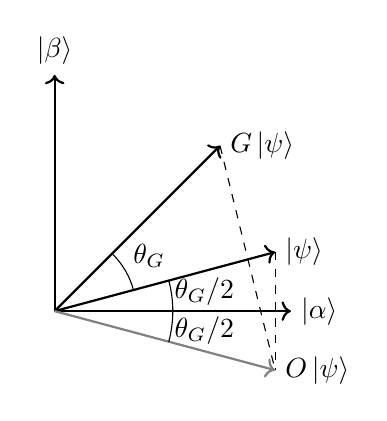
\begin{tikzpicture}
        % 绘制箭头
        \draw[->, thick] (0,0) -- (0,3) node[anchor=south] {$\ket{\beta}$};
        \draw[->, thick] (0,0) -- (2.1,2.1) node[anchor=west] {$G\ket{\psi}$};
        \draw[->, thick] (0,0) -- (2.8,0.75) node[anchor=west] {$\ket{\psi}$};
        \draw[->, thick] (0,0) -- (3,0) node[anchor=west] {$\ket{\alpha}$};
        \draw[->, gray, thick] (0,0) -- (2.8,-0.75) node[anchor=west,black] {$O\ket{\psi}$};
        % 绘制虚线
        \draw[dashed] (2.8,0.75) -- (2.8,-0.75);
        \draw[dashed] (2.1,2.1) -- (2.8,-0.75);
        % 绘制角度标记
        \draw (1.5,0) arc[start angle=0,end angle=15,radius=1.5];
        \draw (1.5,0) arc[start angle=0,end angle=-15,radius=1.5];
        \draw (1,0.27) arc[start angle=15,end angle=45,radius=1];
        % 标记角度
        \node at (1.9,0.25) {$\theta_{G}/2$};
        \node at (1.9,-0.25) {$\theta_{G}/2$};
        \node at (1.2,0.7) {$\theta_{G}$};
    \end{tikzpicture}
    \caption{}
    \label{fig:grover}
\end{figure}

Let $\sin(\theta_{G}/2)=\sqrt{M/N}$,  the angle between $\ket{\psi}$ and $\ket{\alpha}$ is $\theta_{G}/2$. As shown in Figure \ref{fig:grover},  operation $G=DO$ gives us a rotation of angle $\theta_{G}$, we call $G$ the Grover iteration. So we just need applying $R\coloneqq\left\lfloor\frac{\pi-\theta_{G}}{2\theta_{G}}\right\rceil$\footnote{The actual function about $\left\lfloor x\right\rceil$ is to denote the integer closest to the real number $x$.} times Grover iteration on $\ket{\psi}$ to approximate $\ket{\beta}$, if $M\ll N$ we have
\begin{equation}
    G^{R}\ket{\psi}=\cos(\frac{2R+1}{2}\theta_{G})\ket{\alpha}+\sin(\frac{2R+1}{2}\theta_{G})\ket{\beta}\approx\ket{\beta}.
\end{equation}
The angular error is at most $\theta_{G}/2\approx\sqrt{M/N}$.



\subsection{Oracle}

Let's construct the reflection about $\ket{\alpha}$, we call it the oracle. We know that states in the space spanned by $\ket{\alpha}$ and $\ket{\beta}$ can be decomposed into
\begin{equation}
    \ket{x}=\ket{\alpha}\braket{\alpha|x}+\ket{\beta}\braket{\beta|x}
\end{equation}
and we wish
\begin{equation}
    O\ket{x}=\ket{\alpha}\braket{\alpha|x}-\ket{\beta}\braket{\beta|x}.
\end{equation}
We don't know the exact form of $\ket{\alpha}$ and $\ket{\beta}$, so we can not exactly construct the reflection in the whole space, but we just need it to be a reflection in the subspace spanned by $\ket{\alpha}$ and $\ket{\beta}$, may as well construct an operation that identifies each target element to flip it. To construct this, we need a special gate\footnote{Note that the mapping $\ket{x}\xrightarrow{U_{f}}(-1)^{f(x)}\ket{x}$ holds only if the controlled qubit is $\ket{-}$.}
\begin{equation}
    \begin{quantikz}
        \lstick{$\ket{x}$} & \qwbundle{n} & \gate[2][1.7cm]{U_{f}}\gateinput{$x$}\gateoutput{$x$} & \rstick{$(-1)^{f(x)}\ket{x}$} \\
        \lstick{$\ket{-}$} & & \gateinput{$y$}\gateoutput{$y\oplus f(x)$} & \rstick{$\ket{-}$}
    \end{quantikz}
\end{equation}
which gives us a operation $\ket{x}\xrightarrow{U_{f}}(-1)^{f(x)}\ket{x}$. Then we just need to construct the mapping
\begin{equation}
    S(x)=
    \begin{cases}
        1 & x\in T    \\
        0 & x\notin T
    \end{cases}
\end{equation}
such that $U_{S}$ satisfies the properties we need:
\begin{equation}
    \begin{split}
        U_{S}\ket{\beta}  & =-\ket{\beta}  \\
        U_{S}\ket{\alpha} & =\ket{\alpha}.
    \end{split}
\end{equation}
So the $U_{S}$ is the Oracle.



\subsection{Grover iteration}

Then, let's construct the reflection about $\ket{\psi}$. Same as the oracle, we decompose states into
\begin{equation}
    \ket{x}=\ket{\psi}\braket{\psi|x}+\ket{\psi_{\perp}}\braket{\psi_{\perp}|x}
\end{equation}
which $\ket{\psi_{\perp}}=\sqrt{\frac{M}{N}}\ket{\alpha}-\sqrt{\frac{N-M}{N}}\ket{\beta}$, and we wish
\begin{equation}
    D\ket{x}=\ket{\psi}\braket{\psi|x}-\ket{\psi_{\perp}}\braket{\psi_{\perp}|x}.
\end{equation}
But this time, we know $\ket{\psi}$ specifically, operation $2\ket{\psi}\bra{\psi}-I$ is what we need. So we get the construction of the Grover iteration:
\begin{equation}
    G=DO=(2\ket{\psi}\bra{\psi}-I)U_{S}.
\end{equation}
After constructing each sub-operation, the circuit of the algorithm is given here\footnote{The oracle workspace is omitted here.}:
\begin{equation}
    \begin{quantikz}[column sep=0.4cm]
        \lstick{$\ket{0}$} & \qwbundle{n} & \gate{H^{\otimes n}} & \gate[2]{oracle}\gategroup[wires=2,steps=4]{Grover iteration} & \gate{H^{\otimes n}} & \gate{2\ket{0}\bra{0}-I} & \gate{H^{\otimes n}} & \gate[2]{G} & \midstick[2,brackets=none]{$\cdots$} & \gate[2]{G} & \\
        \lstick{$\ket{1}$} & & \gate{H} & & & & & & & &
    \end{quantikz}
\end{equation}
The ellipsis indicates that it is repeated $R$ times.



\subsection{Performance}

Each of the operations in the Grover iteration may be efficiently implemented on a quantum computer. So we just need to focus on the number of Grover iterations.

We already know, in order to rotate $\ket{\psi}$ near $\ket{\beta}$, we need to repeat the Grover iteration
\begin{equation}\label{eq:IterationsGrover}
    R=\left\lfloor\frac{2\arccos\sqrt{M/N}}{\arcsin\sqrt{M/N}}\right\rceil
\end{equation}
times. This is not intuitive enough, so let's sacrifice some precision to find a simpler expression. We know that $R\leq\left\lceil\pi/2\theta_{G}\right\rceil$, and if $M\leq N/2$ we have
\begin{equation}
    \frac{\theta_{G}}{2}\geq\sin\frac{\theta_{G}}{2}=\sqrt{\frac{N}{M}},
\end{equation}
from which we obtain an elegant upper bound on the number of iterations required,
\begin{equation}
    R\leq\left\lceil\frac{\pi}{4}\sqrt{\frac{N}{M}}\right\rceil.
\end{equation}
That is, $R=O(\sqrt{N/M})$ Grover iterations must be performed to obtain a solution to the search problem with high probability, a quadratic improvement over the $O(N/M)$oracle calls required classically.

If $M>N/2$, the quantum search algorithm is not necessary. We can just randomly pick an item from the search space, and then check that it is a solution using the oracle. This approach has a success probability of at least one-half and only requires one consultation with the oracle.



\section{Bounds for Grover's algorithm\label{sec:BoundForGrover}}

\textit{This section is based on the paper\cite{2009Exact}, Here we restrict ourselves to the case $M=1$.}

\subsection{Main idea}

Oracle is at the heart of Grover's algorithm, so let's focus on the oracle and ignore the other operations, we write the state that uses $R$ queries to the oracle as
\begin{equation}
    \ket{\Psi_{x}^{R}}=\prod_{j=1}^{R}U_{j}O_{x}\ket{\psi},
\end{equation}
where $U_{i}$ is some unitary operation and $O_{x}$ is the oracle which marks the target element $x$. To illustrate the effect of oracles, let's replace some of them with unit operations, we write
\begin{equation}
    \ket{\Psi_{x}^{i,R}}=\prod_{j=i+1}^{R}U_{j}O_{x}\prod_{j=1}^{i}U_{j}I\ket{\psi},
\end{equation}
which uses the identity for the first $i$ oracle queries and the oracle for the latter $R-i$ oracle queries. If there is no application oracle,  then the state is independent of the target element and may be denoted as
\begin{equation}
    \ket{\Psi^{R}}=\prod_{j=1}^{R}U_{j}I\ket{\psi}.
\end{equation}
So that we can find the distance changed by oracle, here we use two kinds of metric, euclidean distance and angular distance:
\begin{equation}
    E(\ket{\alpha},\ket{\beta})=\left\|\ket{\alpha}-\ket{\beta}\right\|
    \quad\text{and}\quad
    A(\ket{\alpha},\ket{\beta})=\arccos\frac{\left\lvert \braket{\alpha|\beta}\right\rvert}{\left\|\ket{\alpha}\right\|\left\|\ket{\beta}\right\|}.
\end{equation}
Taking the distance $E$ as an example, if $\Psi_{x}^{R}$ satisfies the properties the output should have
\begin{equation}\label{TheOutputWeWant}
    \left\| \mathsf{\Pi}_{x}\ket{\Psi_{x}^{R}} \right\|^{2} \geq p
\end{equation}
which $\{\mathsf{\Pi}_{j}\}$ is a finite set of orthogonal projectors that sum to the identity and $p$ is the probability we want of outputting the correct element.

We can calculate the number of queries $R$ by dividing $E(\ket{\Psi_{x}^{R}},\ket{\Psi^{R}})$ with the distance changed by oracle\footnote{Note that this is just a loose intuition, which we'll prove in the next subsection.}, that is
\begin{equation}\label{TheNumberForIteration}
    R=\frac{E(\ket{\Psi_{x}^{R}},\ket{\Psi^{R}})}{E(O_{x}\ket{\gamma},\ket{\gamma})}.
\end{equation}
It is important to note that $\ket{\gamma}$ here is not some particular state, we will calculate the mean of the distance changed by oracle on each state.



\subsection{\label{DistanceByOracle}Distance the oracle changes}

First, let's calculate the distance changed by the oracle. Considering the distance of the state before and after $R$ oracle queries, we have
\begin{lemma}
    The average \textcolor{red}{euclidean distance} after $R$ oracle queries is at most
    \begin{equation}
        \frac{1}{N}\sum_{x=1}^{N}\textcolor{red}{E}(\ket{\Psi_{x}^{R}},\ket{\Psi^{R}})\leq 2R\textcolor{red}{\frac{1}{\sqrt{N}}}.
    \end{equation}
\end{lemma}
\begin{proof}
    With triangle inequality,
    \begin{equation*}
        \begin{split}
            \frac{1}{N}\sum_{x=1}^{N}\textcolor{red}{E}(\ket{\Psi_{x}^{R}},\ket{\Psi^{R}})
             & = \frac{1}{N}\sum_{x=1}^{N}\textcolor{red}{E}(\ket{\Psi_{x}^{0,R}},\ket{\Psi_{x}^{R,R}})
            \leq \frac{1}{N}\sum_{x=1}^{N}\sum_{i=1}^{R}\textcolor{red}{E}(\ket{\Psi_{x}^{i-1,R}},\ket{\Psi_{x}^{i,R}}) \\
             & = \frac{1}{N}\sum_{i=1}^{R}\sum_{x=1}^{N}\textcolor{red}{E}(O_{x}\ket{\Psi^{i}},\ket{\Psi^{i}})
            = \frac{1}{N}\sum_{i=1}^{R}\sum_{x=1}^{N}\textcolor{red}{2\left\|\mathsf{\Pi}_{x}\ket{\Psi^{i}}\right\|}    \\
             & \leq 2\sum_{i=1}^{R}\textcolor{red}{\frac{1}{\sqrt{N}}} = 2R\textcolor{red}{\frac{1}{\sqrt{N}}},
        \end{split}
    \end{equation*}
    where the last inequality that needs to be noticed is that
    \begin{equation}\label{Cauchy-Schwarz}
        \left(\sum_{i=1}^{N}a_{i}\right)^{2}=\sum_{i=1}^{N}a_{i}^{2}+2\sum_{i=1}^{N}\sum_{j=1}^{i-1}a_{i}a_{j}\leq N\sum_{i=1}^{N}a_{i}^{2},
    \end{equation}
    that is
    \begin{equation*}
        \sum_{x=1}^{N}\frac{1}{N}\left\|\mathsf{\Pi}_{x}\ket{\Psi^{i}}\right\|\leq \sqrt{\frac{1}{N}\sum_{x=1}^{N}\left\|\mathsf{\Pi}_{x}\ket{\Psi^{i}}\right\|^{2}}=\frac{1}{\sqrt{N}}. \qedhere
    \end{equation*}
\end{proof}
\begin{lemma}
    The average \textcolor{blue}{angular distance} after $R$ oracle queries is at most
    \begin{equation}
        \frac{1}{N}\sum_{x=1}^{N}\textcolor{blue}{A}(\ket{\Psi_{x}^{R}},\ket{\Psi^{R}})\leq 2R\textcolor{blue}{\arcsin(\frac{1}{\sqrt{N}})}.
    \end{equation}
\end{lemma}
\begin{proof}
    With triangle inequality,
    \begin{equation*}
        \begin{split}
            \frac{1}{N}\sum_{x=1}^{N}\textcolor{blue}{A}(\ket{\Psi_{x}^{R}},\ket{\Psi^{R}})
             & = \frac{1}{N}\sum_{x=1}^{N}\textcolor{blue}{A}(\ket{\Psi_{x}^{0,R}},\ket{\Psi_{x}^{R,R}})
            \leq \frac{1}{N}\sum_{x=1}^{N}\sum_{i=1}^{R}\textcolor{blue}{A}(\ket{\Psi_{x}^{i-1,R}},\ket{\Psi_{x}^{i,R}})           \\
             & = \frac{1}{N}\sum_{i=1}^{R}\sum_{x=1}^{N}\textcolor{blue}{A}(O_{x}\ket{\Psi^{i}},\ket{\Psi^{i}})
            = \frac{1}{N}\sum_{i=1}^{R}\sum_{x=1}^{N}\textcolor{blue}{\arccos(\left\lvert\cos(2\theta_{x}^{i})\right\rvert)}       \\
             & \leq 2\sum_{i=1}^{R}\textcolor{blue}{\arcsin(\frac{1}{\sqrt{N}})} = 2R\textcolor{blue}{arcsin(\frac{1}{\sqrt{N}})},
        \end{split}
    \end{equation*}
    where has $\theta_{x}^{i}=A(\ket{\Psi^{i}},\ket{x_{\perp}})=\arcsin\left\| \mathsf{\Pi}_{x}\ket{\Psi^{i}}\right\|$. And where the last inequality still needs to notice the rescaling provided by equation \ref{Cauchy-Schwarz}, that is
    \begin{equation*}
        \sum_{x=1}^{N}\frac{1}{N}\arcsin\left\|\mathsf{\Pi}_{x}\ket{\Psi^{i}}\right\|\leq\arcsin\sum_{x=1}^{N}\frac{1}{N}\left\|\mathsf{\Pi}_{x}\ket{\Psi^{i}}\right\|\leq\arcsin\frac{1}{\sqrt{N}},
    \end{equation*}
    where also need notice that $\sum_{x=1}^{N}\frac{1}{N}\arcsin a_{i}\leq\arcsin\sum_{x=1}^{N}\frac{1}{N}a_{i}$ which $a_{i}\in\left[0,\frac{\pi}{2}\right]$.
\end{proof}
According to the theorem, the distance changed by each oracle query can only add up linearly.



\subsection{\label{DistanceWhenWeNeed}Distance when the output is we need}

Then, let's calculate the distance when equation \ref{TheOutputWeWant} is satisfied.
\begin{lemma}
    Suppose that the algorithm correctly outputs $y$ with probability at least $p$ after $R$ queries, given oracle $O_{y}$. Then the average Euclidean distance is at least
    \begin{equation}
        \frac{1}{N}\sum_{x=1}^{N}E(\ket{\Psi_{x}^{R}},\ket{\Psi^{R}})\geq \frac{1}{\sqrt{2}}\left(\sqrt{p}-\sqrt{1-p}+1-\frac{2}{\sqrt{N}}\right).
    \end{equation}
\end{lemma}
\begin{proof}
    For a certain $x$, we have
    \begin{equation*}
        \begin{split}
            E(\ket{\Psi_{x}^{R}},\ket{\Psi^{R}})
             & \geq \frac{1}{\sqrt{2}}\left(\left\|\mathsf{\Pi}_{x}\left(\ket{\Psi_{x}^{R}}-\ket{\Psi^{R}}\right)\right\|+\left\|\mathsf{\Pi}_{x}^{\perp}\left(\ket{\Psi_{x}^{R}}-\ket{\Psi^{R}}\right)\right\|\right)                                             \\
             & \geq \frac{1}{\sqrt{2}}\left(\left\|\mathsf{\Pi}_{x}\ket{\Psi_{x}^{R}}\right\|-\left\|\mathsf{\Pi}_{x}\ket{\Psi^{R}}\right\|+\left\|\mathsf{\Pi}_{x}^{\perp}\ket{\Psi^{R}}\right\|-\left\|\mathsf{\Pi}_{x}^{\perp}\ket{\Psi_{x}^{R}}\right\|\right) \\
             & \geq \frac{1}{\sqrt{2}}\left(\left\|\mathsf{\Pi}_{x}\ket{\Psi_{x}^{R}}\right\|-\left\|\mathsf{\Pi}_{x}^{\perp}\ket{\Psi_{x}^{R}}\right\|+1-2\left\|\mathsf{\Pi}_{x}\ket{\Psi^{R}}\right\|\right)                                                    \\
             & \geq \frac{1}{\sqrt{2}}\left(\sqrt{p}-\sqrt{1-p}+1-2\left\|\mathsf{\Pi}_{x}\ket{\Psi^{R}}\right\|\right),
        \end{split}
    \end{equation*}
    where the last inequality from the success probability is at least $p$. To eliminate the last term, consider a traversal of $x$
    \begin{equation*}
        \frac{1}{N}\sum_{x=1}^{N}E(\ket{\Psi_{x}^{R}},\ket{\Psi^{R}})
        \geq \frac{1}{\sqrt{2}}\left(\sqrt{p}-\sqrt{1-p}+1-\frac{2}{N}\sum_{x=1}^{N}\left\|\mathsf{\Pi}_{x}\ket{\Psi^{R}}\right\|\right)
        \geq \frac{1}{\sqrt{2}}\left(\sqrt{p}-\sqrt{1-p}+1-\frac{2}{\sqrt{N}}\right),
    \end{equation*}
    where the last inequality uses the equation \ref{Cauchy-Schwarz} again.
\end{proof}
\begin{lemma}
    Suppose that the algorithm correctly outputs $y$ with probability at least $p$ after $R$ queries, given oracle $O_{y}$. Then the average angular distance is at least
    \begin{equation}
        \frac{1}{N}\sum_{x=1}^{N}A(\ket{\Psi_{x}^{R}},\ket{\Psi^{R}})\geq \arcsin\sqrt{p}-\arcsin\frac{1}{\sqrt{N}}.
    \end{equation}
\end{lemma}
\begin{proof}
    For a certain $x$, we have
    \begin{equation*}
        \begin{split}
            A(\ket{\Psi_{x}^{R}},\ket{\Psi^{R}})
             & = \arccos\left(\left\lvert \braket{\Psi_{x}^{R}|\Psi^{R}}\right\rvert\right)                                                                                                                                                                  \\
             & = \arccos\left(\bra{\Psi_{x}^{R}}(\mathsf{\Pi}_{x}+\mathsf{\Pi}_{x}^{\perp})^{\dagger}(\mathsf{\Pi}_{x}+\mathsf{\Pi}_{x}^{\perp})\ket{\Psi^{R}}\right)                                                                                        \\
             & = \arccos\left(\left\|\mathsf{\Pi}_{x}\ket{\Psi_{x}^{R}}\right\|\cdot\left\|\mathsf{\Pi}_{x}\ket{\Psi^{R}}\right\|+\left\|\mathsf{\Pi}_{x}^{\perp}\ket{\Psi_{x}^{R}}\right\|\cdot\left\|\mathsf{\Pi}_{x}^{\perp}\ket{\Psi^{R}}\right\|\right) \\
             & = \arccos\left(\sin\phi_{x}^{R}\sin\theta_{x}^{R}+\cos\phi_{x}^{R}\cos\theta_{x}^{R}\right)                                                                                                                                                   \\
             & = \phi_{x}^{R}-\theta_{x}^{R} \geq \arcsin\sqrt{p}-\theta_{x}^{R},
        \end{split}
    \end{equation*}
    where has $\phi_{x}^{i}=\arcsin\left\| \mathsf{\Pi}_{x}\ket{\Psi_{x}^{i}}\right\|$ and still has $\theta_{x}^{i}=\arcsin\left\| \mathsf{\Pi}_{x}\ket{\Psi^{i}}\right\|$, and where the last inequality from the success probability being at least $p$. Just like the last proof, consider a traversal of $x$
    \begin{equation*}
        \frac{1}{N}\sum_{x=1}^{N}A(\ket{\Psi_{x}^{R}},\ket{\Psi^{R}})
        \geq \arcsin\sqrt{p}-\frac{1}{N}\sum_{x=1}^{N}\theta_{x}^{R}
        \geq \arcsin\sqrt{p}-\arcsin\frac{1}{\sqrt{N}},
    \end{equation*}
    where the last inequality uses the equation \ref{Cauchy-Schwarz} again.
\end{proof}



\subsection{Lower bound of Grover iterations}

From section \ref{DistanceByOracle} and section \ref{DistanceWhenWeNeed}, we obtain the two parts required for equation \ref{TheNumberForIteration} to compute the number of iterations: the upper bound of the distance changed by oracle and the lower bound of the distance when the output is we need. So we have the lower bound on the number of iterations for both versions
\begin{theorem}
    The unordered search problem with success probability $p>0$ requires at least $R$ queries, where
    \begin{equation}
        R =\frac{\sqrt{N}}{2\sqrt{2}}\left(\sqrt{p}-\sqrt{1-p}+1-\frac{2}{\sqrt{N}}\right).
    \end{equation}
\end{theorem}
\begin{theorem}
    The unordered search problem with success probability $p>0$ requires at least $R$ queries, where
    \begin{equation}
        R =\frac{\arcsin\sqrt{p}-\arcsin\frac{1}{\sqrt{N}}}{2\arcsin\frac{1}{\sqrt{N}}}.
    \end{equation}
\end{theorem}
In the case of Euclidean distances, we conclude that Grover's algorithm is asymptotically optimal, and in the case of angular distances, Grover's algorithm is exactly optimal.



\section{Long's algorithm}

\textit{This section is based on the paper\cite{Long_2001}.}

\subsection{\label{subsec:LongMainIdea}Main idea}

Although Grover's algorithm is already accurate enough when the number of elements is large, for instance in deciphering the DES code where $N = 256$ the deviation is only $3\times 10^{-9}$. But in problems where certainly is vital, especially when the dimension is not so big, using a searching algorithm with certainty becomes important. Let's make some improvements to the Grover's algorithm.

In the Grover's algorithm\footnote{The notation of section \ref{subsec:GroverMainIdea} is followed here.} we construct rotations in the space spanned by $\ket{\alpha}$ and $\ket{\beta}$, we wasted the degree of freedom of their relative phase, so we may as well extend\footnote{For convenience, the oracle can be written as $(I-2\ket{\beta}\bra{\beta})$ when discussing only in the subspace spanned by $\ket{\alpha}$ and $\ket{\beta}$.} $G=DO=(I-2\ket{\psi_{\perp}}\bra{\psi_{\perp}})(I-2\ket{\beta}\bra{\beta})$ to
\begin{equation}
    \begin{split}
        I_{D} & = I+(e^{-i\phi}-1)\ket{\psi_{\perp}}\bra{\psi_{\perp}} = e^{-i\phi}(I+(e^{i\phi}-1)\ket{\psi}\bra{\psi})                   \\
        I_{O} & = I+(e^{i\phi}-1)\ket{\beta}\bra{\beta}                                                                                    \\
        Q     & = I_{D}I_{O} = e^{-i\phi}H^{\otimes n}(I+(e^{i\phi}-1)\ket{0}\bra{0})H^{\otimes n}(I+(e^{i\phi}-1)\ket{\beta}\bra{\beta}).
    \end{split}
\end{equation}
Intuitively, if we want $Q$ to make $\ket{\psi}$ go to $\ket{\beta}$, we should have the axis of rotation at the same angle as $\ket{\psi}$ and $\ket{\beta}$. From corollary \ref{cor:CompositionOfRotation}, if the angle of $I_{O}$ is $-\phi$, the angle of $I_{W}$ has to be $\phi$. As a generalization of Grover's algorithm, it can be seen that if we set $\phi=\pi$, then $Q$ degenerates to $G$.
\begin{figure}[h]
    \centering
    \resizebox{0.5\textwidth}{!}{%% Creator: Matplotlib, PGF backend
%%
%% To include the figure in your LaTeX document, write
%%   \input{<filename>.pgf}
%%
%% Make sure the required packages are loaded in your preamble
%%   \usepackage{pgf}
%%
%% Also ensure that all the required font packages are loaded; for instance,
%% the lmodern package is sometimes necessary when using math font.
%%   \usepackage{lmodern}
%%
%% Figures using additional raster images can only be included by \input if
%% they are in the same directory as the main LaTeX file. For loading figures
%% from other directories you can use the `import` package
%%   \usepackage{import}
%%
%% and then include the figures with
%%   \import{<path to file>}{<filename>.pgf}
%%
%% Matplotlib used the following preamble
%%   \def\mathdefault#1{#1}
%%   \everymath=\expandafter{\the\everymath\displaystyle}
%%   
%%   \ifdefined\pdftexversion\else  % non-pdftex case.
%%     \usepackage{fontspec}
%%   \fi
%%   \makeatletter\@ifpackageloaded{underscore}{}{\usepackage[strings]{underscore}}\makeatother
%%
\begingroup%
\makeatletter%
\begin{pgfpicture}%
\pgfpathrectangle{\pgfpointorigin}{\pgfqpoint{9.000000in}{9.000000in}}%
\pgfusepath{use as bounding box, clip}%
\begin{pgfscope}%
\pgfsetbuttcap%
\pgfsetmiterjoin%
\definecolor{currentfill}{rgb}{1.000000,1.000000,1.000000}%
\pgfsetfillcolor{currentfill}%
\pgfsetlinewidth{0.000000pt}%
\definecolor{currentstroke}{rgb}{1.000000,1.000000,1.000000}%
\pgfsetstrokecolor{currentstroke}%
\pgfsetdash{}{0pt}%
\pgfpathmoveto{\pgfqpoint{0.000000in}{0.000000in}}%
\pgfpathlineto{\pgfqpoint{9.000000in}{0.000000in}}%
\pgfpathlineto{\pgfqpoint{9.000000in}{9.000000in}}%
\pgfpathlineto{\pgfqpoint{0.000000in}{9.000000in}}%
\pgfpathlineto{\pgfqpoint{0.000000in}{0.000000in}}%
\pgfpathclose%
\pgfusepath{fill}%
\end{pgfscope}%
\begin{pgfscope}%
\pgfsetbuttcap%
\pgfsetmiterjoin%
\definecolor{currentfill}{rgb}{1.000000,1.000000,1.000000}%
\pgfsetfillcolor{currentfill}%
\pgfsetlinewidth{0.000000pt}%
\definecolor{currentstroke}{rgb}{0.000000,0.000000,0.000000}%
\pgfsetstrokecolor{currentstroke}%
\pgfsetstrokeopacity{0.000000}%
\pgfsetdash{}{0pt}%
\pgfpathmoveto{\pgfqpoint{0.000000in}{0.000000in}}%
\pgfpathlineto{\pgfqpoint{9.000000in}{0.000000in}}%
\pgfpathlineto{\pgfqpoint{9.000000in}{9.000000in}}%
\pgfpathlineto{\pgfqpoint{0.000000in}{9.000000in}}%
\pgfpathlineto{\pgfqpoint{0.000000in}{0.000000in}}%
\pgfpathclose%
\pgfusepath{fill}%
\end{pgfscope}%
\begin{pgfscope}%
\pgfpathrectangle{\pgfqpoint{0.000000in}{0.000000in}}{\pgfqpoint{9.000000in}{9.000000in}}%
\pgfusepath{clip}%
\pgfsetrectcap%
\pgfsetroundjoin%
\pgfsetlinewidth{1.003750pt}%
\definecolor{currentstroke}{rgb}{0.501961,0.501961,0.501961}%
\pgfsetstrokecolor{currentstroke}%
\pgfsetdash{}{0pt}%
\pgfpathmoveto{\pgfqpoint{0.941880in}{4.567061in}}%
\pgfpathlineto{\pgfqpoint{8.423309in}{4.677990in}}%
\pgfusepath{stroke}%
\end{pgfscope}%
\begin{pgfscope}%
\pgfpathrectangle{\pgfqpoint{0.000000in}{0.000000in}}{\pgfqpoint{9.000000in}{9.000000in}}%
\pgfusepath{clip}%
\pgfsetrectcap%
\pgfsetroundjoin%
\pgfsetlinewidth{1.003750pt}%
\definecolor{currentstroke}{rgb}{0.501961,0.501961,0.501961}%
\pgfsetstrokecolor{currentstroke}%
\pgfsetdash{}{0pt}%
\pgfpathmoveto{\pgfqpoint{3.760700in}{4.904158in}}%
\pgfpathlineto{\pgfqpoint{5.359908in}{4.379332in}}%
\pgfusepath{stroke}%
\end{pgfscope}%
\begin{pgfscope}%
\pgfpathrectangle{\pgfqpoint{0.000000in}{0.000000in}}{\pgfqpoint{9.000000in}{9.000000in}}%
\pgfusepath{clip}%
\pgfsetrectcap%
\pgfsetroundjoin%
\pgfsetlinewidth{1.003750pt}%
\definecolor{currentstroke}{rgb}{0.501961,0.501961,0.501961}%
\pgfsetstrokecolor{currentstroke}%
\pgfsetdash{}{0pt}%
\pgfpathmoveto{\pgfqpoint{4.621622in}{0.786643in}}%
\pgfpathlineto{\pgfqpoint{4.621622in}{8.414782in}}%
\pgfusepath{stroke}%
\end{pgfscope}%
\begin{pgfscope}%
\pgfpathrectangle{\pgfqpoint{0.000000in}{0.000000in}}{\pgfqpoint{9.000000in}{9.000000in}}%
\pgfusepath{clip}%
\pgfsetrectcap%
\pgfsetroundjoin%
\pgfsetlinewidth{1.003750pt}%
\definecolor{currentstroke}{rgb}{0.501961,0.501961,0.501961}%
\pgfsetstrokecolor{currentstroke}%
\pgfsetdash{}{0pt}%
\pgfpathmoveto{\pgfqpoint{8.423309in}{4.677990in}}%
\pgfpathlineto{\pgfqpoint{8.456694in}{4.642676in}}%
\pgfpathlineto{\pgfqpoint{8.424049in}{4.607721in}}%
\pgfpathlineto{\pgfqpoint{8.327917in}{4.573704in}}%
\pgfpathlineto{\pgfqpoint{8.171759in}{4.541157in}}%
\pgfpathlineto{\pgfqpoint{7.959780in}{4.510554in}}%
\pgfpathlineto{\pgfqpoint{7.696779in}{4.482316in}}%
\pgfpathlineto{\pgfqpoint{7.388006in}{4.456807in}}%
\pgfpathlineto{\pgfqpoint{7.039046in}{4.434338in}}%
\pgfpathlineto{\pgfqpoint{6.655722in}{4.415168in}}%
\pgfpathlineto{\pgfqpoint{6.244020in}{4.399508in}}%
\pgfpathlineto{\pgfqpoint{5.810030in}{4.387522in}}%
\pgfpathlineto{\pgfqpoint{5.359908in}{4.379332in}}%
\pgfpathlineto{\pgfqpoint{4.899847in}{4.375020in}}%
\pgfpathlineto{\pgfqpoint{4.436055in}{4.374627in}}%
\pgfpathlineto{\pgfqpoint{3.974751in}{4.378157in}}%
\pgfpathlineto{\pgfqpoint{3.522145in}{4.385577in}}%
\pgfpathlineto{\pgfqpoint{3.084435in}{4.396812in}}%
\pgfpathlineto{\pgfqpoint{2.667785in}{4.411749in}}%
\pgfpathlineto{\pgfqpoint{2.278303in}{4.430233in}}%
\pgfpathlineto{\pgfqpoint{1.921998in}{4.452061in}}%
\pgfpathlineto{\pgfqpoint{1.604731in}{4.476985in}}%
\pgfpathlineto{\pgfqpoint{1.332144in}{4.504705in}}%
\pgfpathlineto{\pgfqpoint{1.109560in}{4.534866in}}%
\pgfpathlineto{\pgfqpoint{0.941880in}{4.567061in}}%
\pgfusepath{stroke}%
\end{pgfscope}%
\begin{pgfscope}%
\pgfpathrectangle{\pgfqpoint{0.000000in}{0.000000in}}{\pgfqpoint{9.000000in}{9.000000in}}%
\pgfusepath{clip}%
\pgfsetrectcap%
\pgfsetroundjoin%
\pgfsetlinewidth{1.003750pt}%
\definecolor{currentstroke}{rgb}{0.501961,0.501961,0.501961}%
\pgfsetstrokecolor{currentstroke}%
\pgfsetdash{}{0pt}%
\pgfpathmoveto{\pgfqpoint{5.359908in}{4.379332in}}%
\pgfpathlineto{\pgfqpoint{5.353552in}{4.843757in}}%
\pgfpathlineto{\pgfqpoint{5.335544in}{5.305164in}}%
\pgfpathlineto{\pgfqpoint{5.306087in}{5.757304in}}%
\pgfpathlineto{\pgfqpoint{5.265501in}{6.193950in}}%
\pgfpathlineto{\pgfqpoint{5.214229in}{6.608913in}}%
\pgfpathlineto{\pgfqpoint{5.152838in}{6.996075in}}%
\pgfpathlineto{\pgfqpoint{5.082032in}{7.349423in}}%
\pgfpathlineto{\pgfqpoint{5.002654in}{7.663111in}}%
\pgfpathlineto{\pgfqpoint{4.915698in}{7.931529in}}%
\pgfpathlineto{\pgfqpoint{4.822312in}{8.149403in}}%
\pgfpathlineto{\pgfqpoint{4.723799in}{8.311902in}}%
\pgfpathlineto{\pgfqpoint{4.621622in}{8.414782in}}%
\pgfpathlineto{\pgfqpoint{4.517389in}{8.454530in}}%
\pgfpathlineto{\pgfqpoint{4.412848in}{8.428536in}}%
\pgfpathlineto{\pgfqpoint{4.309856in}{8.335259in}}%
\pgfpathlineto{\pgfqpoint{4.210354in}{8.174393in}}%
\pgfpathlineto{\pgfqpoint{4.116325in}{7.947019in}}%
\pgfpathlineto{\pgfqpoint{4.029741in}{7.655718in}}%
\pgfpathlineto{\pgfqpoint{3.952509in}{7.304648in}}%
\pgfpathlineto{\pgfqpoint{3.886405in}{6.899555in}}%
\pgfpathlineto{\pgfqpoint{3.833011in}{6.447714in}}%
\pgfpathlineto{\pgfqpoint{3.793651in}{5.957804in}}%
\pgfpathlineto{\pgfqpoint{3.769331in}{5.439692in}}%
\pgfpathlineto{\pgfqpoint{3.760700in}{4.904158in}}%
\pgfusepath{stroke}%
\end{pgfscope}%
\begin{pgfscope}%
\pgfpathrectangle{\pgfqpoint{0.000000in}{0.000000in}}{\pgfqpoint{9.000000in}{9.000000in}}%
\pgfusepath{clip}%
\pgfsetrectcap%
\pgfsetroundjoin%
\pgfsetlinewidth{1.505625pt}%
\definecolor{currentstroke}{rgb}{0.000000,0.500000,0.000000}%
\pgfsetstrokecolor{currentstroke}%
\pgfsetstrokeopacity{0.300000}%
\pgfsetdash{}{0pt}%
\pgfpathmoveto{\pgfqpoint{4.621622in}{7.470375in}}%
\pgfpathlineto{\pgfqpoint{4.070138in}{7.802919in}}%
\pgfusepath{stroke}%
\end{pgfscope}%
\begin{pgfscope}%
\pgfpathrectangle{\pgfqpoint{0.000000in}{0.000000in}}{\pgfqpoint{9.000000in}{9.000000in}}%
\pgfusepath{clip}%
\pgfsetrectcap%
\pgfsetroundjoin%
\pgfsetlinewidth{1.505625pt}%
\definecolor{currentstroke}{rgb}{0.000000,0.500000,0.000000}%
\pgfsetstrokecolor{currentstroke}%
\pgfsetstrokeopacity{0.300000}%
\pgfsetdash{}{0pt}%
\pgfpathmoveto{\pgfqpoint{4.621622in}{7.470375in}}%
\pgfpathlineto{\pgfqpoint{6.949473in}{7.362597in}}%
\pgfusepath{stroke}%
\end{pgfscope}%
\begin{pgfscope}%
\pgfpathrectangle{\pgfqpoint{0.000000in}{0.000000in}}{\pgfqpoint{9.000000in}{9.000000in}}%
\pgfusepath{clip}%
\pgfsetrectcap%
\pgfsetroundjoin%
\pgfsetlinewidth{1.505625pt}%
\definecolor{currentstroke}{rgb}{0.000000,0.000000,1.000000}%
\pgfsetstrokecolor{currentstroke}%
\pgfsetstrokeopacity{0.300000}%
\pgfsetdash{}{0pt}%
\pgfpathmoveto{\pgfqpoint{4.444558in}{5.643032in}}%
\pgfpathlineto{\pgfqpoint{6.949473in}{7.362597in}}%
\pgfusepath{stroke}%
\end{pgfscope}%
\begin{pgfscope}%
\pgfpathrectangle{\pgfqpoint{0.000000in}{0.000000in}}{\pgfqpoint{9.000000in}{9.000000in}}%
\pgfusepath{clip}%
\pgfsetrectcap%
\pgfsetroundjoin%
\pgfsetlinewidth{1.505625pt}%
\definecolor{currentstroke}{rgb}{0.000000,0.000000,1.000000}%
\pgfsetstrokecolor{currentstroke}%
\pgfsetstrokeopacity{0.300000}%
\pgfsetdash{}{0pt}%
\pgfpathmoveto{\pgfqpoint{4.444558in}{5.643032in}}%
\pgfpathlineto{\pgfqpoint{5.271299in}{3.523047in}}%
\pgfusepath{stroke}%
\end{pgfscope}%
\begin{pgfscope}%
\pgfpathrectangle{\pgfqpoint{0.000000in}{0.000000in}}{\pgfqpoint{9.000000in}{9.000000in}}%
\pgfusepath{clip}%
\pgfsetrectcap%
\pgfsetroundjoin%
\pgfsetlinewidth{1.505625pt}%
\definecolor{currentstroke}{rgb}{1.000000,0.000000,0.000000}%
\pgfsetstrokecolor{currentstroke}%
\pgfsetstrokeopacity{0.300000}%
\pgfsetdash{}{0pt}%
\pgfpathmoveto{\pgfqpoint{4.070138in}{7.802919in}}%
\pgfpathlineto{\pgfqpoint{3.969555in}{4.510629in}}%
\pgfusepath{stroke}%
\end{pgfscope}%
\begin{pgfscope}%
\pgfpathrectangle{\pgfqpoint{0.000000in}{0.000000in}}{\pgfqpoint{9.000000in}{9.000000in}}%
\pgfusepath{clip}%
\pgfsetrectcap%
\pgfsetroundjoin%
\pgfsetlinewidth{1.505625pt}%
\definecolor{currentstroke}{rgb}{1.000000,0.000000,0.000000}%
\pgfsetstrokecolor{currentstroke}%
\pgfsetstrokeopacity{0.300000}%
\pgfsetdash{}{0pt}%
\pgfpathmoveto{\pgfqpoint{5.271299in}{3.523047in}}%
\pgfpathlineto{\pgfqpoint{3.969555in}{4.510629in}}%
\pgfusepath{stroke}%
\end{pgfscope}%
\begin{pgfscope}%
\pgfpathrectangle{\pgfqpoint{0.000000in}{0.000000in}}{\pgfqpoint{9.000000in}{9.000000in}}%
\pgfusepath{clip}%
\pgfsetrectcap%
\pgfsetroundjoin%
\pgfsetlinewidth{1.505625pt}%
\definecolor{currentstroke}{rgb}{1.000000,0.000000,0.000000}%
\pgfsetstrokecolor{currentstroke}%
\pgfsetstrokeopacity{0.300000}%
\pgfsetdash{}{0pt}%
\pgfpathmoveto{\pgfqpoint{4.621622in}{0.786643in}}%
\pgfpathlineto{\pgfqpoint{3.969555in}{4.510629in}}%
\pgfusepath{stroke}%
\end{pgfscope}%
\begin{pgfscope}%
\pgfpathrectangle{\pgfqpoint{0.000000in}{0.000000in}}{\pgfqpoint{9.000000in}{9.000000in}}%
\pgfusepath{clip}%
\pgfsetrectcap%
\pgfsetroundjoin%
\pgfsetlinewidth{1.003750pt}%
\definecolor{currentstroke}{rgb}{0.501961,0.501961,0.501961}%
\pgfsetstrokecolor{currentstroke}%
\pgfsetdash{}{0pt}%
\pgfpathmoveto{\pgfqpoint{0.941880in}{4.567061in}}%
\pgfpathlineto{\pgfqpoint{0.833440in}{4.600825in}}%
\pgfpathlineto{\pgfqpoint{0.787863in}{4.635637in}}%
\pgfpathlineto{\pgfqpoint{0.807888in}{4.670928in}}%
\pgfpathlineto{\pgfqpoint{0.895200in}{4.706082in}}%
\pgfpathlineto{\pgfqpoint{1.050258in}{4.740448in}}%
\pgfpathlineto{\pgfqpoint{1.272141in}{4.773354in}}%
\pgfpathlineto{\pgfqpoint{1.558422in}{4.804120in}}%
\pgfpathlineto{\pgfqpoint{1.905088in}{4.832078in}}%
\pgfpathlineto{\pgfqpoint{2.306520in}{4.856596in}}%
\pgfpathlineto{\pgfqpoint{2.755543in}{4.877097in}}%
\pgfpathlineto{\pgfqpoint{3.243547in}{4.893083in}}%
\pgfpathlineto{\pgfqpoint{3.760700in}{4.904158in}}%
\pgfpathlineto{\pgfqpoint{4.296219in}{4.910039in}}%
\pgfpathlineto{\pgfqpoint{4.838712in}{4.910576in}}%
\pgfpathlineto{\pgfqpoint{5.376551in}{4.905756in}}%
\pgfpathlineto{\pgfqpoint{5.898264in}{4.895702in}}%
\pgfpathlineto{\pgfqpoint{6.392920in}{4.880669in}}%
\pgfpathlineto{\pgfqpoint{6.850470in}{4.861035in}}%
\pgfpathlineto{\pgfqpoint{7.262043in}{4.837276in}}%
\pgfpathlineto{\pgfqpoint{7.620163in}{4.809957in}}%
\pgfpathlineto{\pgfqpoint{7.918893in}{4.779700in}}%
\pgfpathlineto{\pgfqpoint{8.153899in}{4.747168in}}%
\pgfpathlineto{\pgfqpoint{8.322443in}{4.713040in}}%
\pgfpathlineto{\pgfqpoint{8.423309in}{4.677990in}}%
\pgfusepath{stroke}%
\end{pgfscope}%
\begin{pgfscope}%
\pgfpathrectangle{\pgfqpoint{0.000000in}{0.000000in}}{\pgfqpoint{9.000000in}{9.000000in}}%
\pgfusepath{clip}%
\pgfsetrectcap%
\pgfsetroundjoin%
\pgfsetlinewidth{1.003750pt}%
\definecolor{currentstroke}{rgb}{0.501961,0.501961,0.501961}%
\pgfsetstrokecolor{currentstroke}%
\pgfsetdash{}{0pt}%
\pgfpathmoveto{\pgfqpoint{3.760700in}{4.904158in}}%
\pgfpathlineto{\pgfqpoint{3.768010in}{4.362557in}}%
\pgfpathlineto{\pgfqpoint{3.791109in}{3.826450in}}%
\pgfpathlineto{\pgfqpoint{3.829442in}{3.307217in}}%
\pgfpathlineto{\pgfqpoint{3.882075in}{2.815679in}}%
\pgfpathlineto{\pgfqpoint{3.947736in}{2.361768in}}%
\pgfpathlineto{\pgfqpoint{4.024869in}{1.954234in}}%
\pgfpathlineto{\pgfqpoint{4.111693in}{1.600438in}}%
\pgfpathlineto{\pgfqpoint{4.206273in}{1.306214in}}%
\pgfpathlineto{\pgfqpoint{4.306585in}{1.075803in}}%
\pgfpathlineto{\pgfqpoint{4.410580in}{0.911868in}}%
\pgfpathlineto{\pgfqpoint{4.516238in}{0.815563in}}%
\pgfpathlineto{\pgfqpoint{4.621622in}{0.786643in}}%
\pgfpathlineto{\pgfqpoint{4.724905in}{0.823618in}}%
\pgfpathlineto{\pgfqpoint{4.824406in}{0.923916in}}%
\pgfpathlineto{\pgfqpoint{4.918606in}{1.084053in}}%
\pgfpathlineto{\pgfqpoint{5.006154in}{1.299801in}}%
\pgfpathlineto{\pgfqpoint{5.085874in}{1.566341in}}%
\pgfpathlineto{\pgfqpoint{5.156759in}{1.878401in}}%
\pgfpathlineto{\pgfqpoint{5.217969in}{2.230370in}}%
\pgfpathlineto{\pgfqpoint{5.268820in}{2.616397in}}%
\pgfpathlineto{\pgfqpoint{5.308774in}{3.030464in}}%
\pgfpathlineto{\pgfqpoint{5.337432in}{3.466444in}}%
\pgfpathlineto{\pgfqpoint{5.354526in}{3.918144in}}%
\pgfpathlineto{\pgfqpoint{5.359908in}{4.379332in}}%
\pgfusepath{stroke}%
\end{pgfscope}%
\begin{pgfscope}%
\pgfpathrectangle{\pgfqpoint{0.000000in}{0.000000in}}{\pgfqpoint{9.000000in}{9.000000in}}%
\pgfusepath{clip}%
\pgfsetbuttcap%
\pgfsetroundjoin%
\definecolor{currentfill}{rgb}{0.000000,0.000000,1.000000}%
\pgfsetfillcolor{currentfill}%
\pgfsetfillopacity{0.700000}%
\pgfsetlinewidth{1.003750pt}%
\definecolor{currentstroke}{rgb}{0.000000,0.000000,1.000000}%
\pgfsetstrokecolor{currentstroke}%
\pgfsetstrokeopacity{0.700000}%
\pgfsetdash{}{0pt}%
\pgfpathmoveto{\pgfqpoint{6.910189in}{7.323313in}}%
\pgfpathlineto{\pgfqpoint{6.988756in}{7.323313in}}%
\pgfpathlineto{\pgfqpoint{6.988756in}{7.401880in}}%
\pgfpathlineto{\pgfqpoint{6.910189in}{7.401880in}}%
\pgfpathlineto{\pgfqpoint{6.910189in}{7.323313in}}%
\pgfpathclose%
\pgfusepath{stroke,fill}%
\end{pgfscope}%
\begin{pgfscope}%
\pgfpathrectangle{\pgfqpoint{0.000000in}{0.000000in}}{\pgfqpoint{9.000000in}{9.000000in}}%
\pgfusepath{clip}%
\pgfsetbuttcap%
\pgfsetroundjoin%
\definecolor{currentfill}{rgb}{0.000000,0.000000,1.000000}%
\pgfsetfillcolor{currentfill}%
\pgfsetfillopacity{0.700000}%
\pgfsetlinewidth{1.003750pt}%
\definecolor{currentstroke}{rgb}{0.000000,0.000000,1.000000}%
\pgfsetstrokecolor{currentstroke}%
\pgfsetstrokeopacity{0.700000}%
\pgfsetdash{}{0pt}%
\pgfpathmoveto{\pgfqpoint{6.910189in}{7.323313in}}%
\pgfpathlineto{\pgfqpoint{6.988756in}{7.323313in}}%
\pgfpathlineto{\pgfqpoint{6.988756in}{7.401880in}}%
\pgfpathlineto{\pgfqpoint{6.910189in}{7.401880in}}%
\pgfpathlineto{\pgfqpoint{6.910189in}{7.323313in}}%
\pgfpathclose%
\pgfusepath{stroke,fill}%
\end{pgfscope}%
\begin{pgfscope}%
\pgfpathrectangle{\pgfqpoint{0.000000in}{0.000000in}}{\pgfqpoint{9.000000in}{9.000000in}}%
\pgfusepath{clip}%
\pgfsetroundcap%
\pgfsetroundjoin%
\pgfsetlinewidth{3.011250pt}%
\definecolor{currentstroke}{rgb}{0.000000,0.500000,0.000000}%
\pgfsetstrokecolor{currentstroke}%
\pgfsetdash{}{0pt}%
\pgfpathmoveto{\pgfqpoint{4.621622in}{4.649375in}}%
\pgfpathquadraticcurveto{\pgfqpoint{4.621622in}{6.518188in}}{\pgfqpoint{4.621622in}{8.340418in}}%
\pgfusepath{stroke}%
\end{pgfscope}%
\begin{pgfscope}%
\pgfpathrectangle{\pgfqpoint{0.000000in}{0.000000in}}{\pgfqpoint{9.000000in}{9.000000in}}%
\pgfusepath{clip}%
\pgfsetroundcap%
\pgfsetroundjoin%
\definecolor{currentfill}{rgb}{0.000000,0.500000,0.000000}%
\pgfsetfillcolor{currentfill}%
\pgfsetlinewidth{3.011250pt}%
\definecolor{currentstroke}{rgb}{0.000000,0.500000,0.000000}%
\pgfsetstrokecolor{currentstroke}%
\pgfsetdash{}{0pt}%
\pgfpathmoveto{\pgfqpoint{4.566066in}{8.229306in}}%
\pgfpathlineto{\pgfqpoint{4.621622in}{8.340418in}}%
\pgfpathlineto{\pgfqpoint{4.677177in}{8.229306in}}%
\pgfpathlineto{\pgfqpoint{4.566066in}{8.229306in}}%
\pgfpathclose%
\pgfusepath{stroke,fill}%
\end{pgfscope}%
\begin{pgfscope}%
\definecolor{textcolor}{rgb}{0.000000,0.000000,0.000000}%
\pgfsetstrokecolor{textcolor}%
\pgfsetfillcolor{textcolor}%
\pgftext[x=4.621622in,y=8.414782in,,]{\color{textcolor}{\rmfamily\fontsize{20.000000}{24.000000}\selectfont\catcode`\^=\active\def^{\ifmmode\sp\else\^{}\fi}\catcode`\%=\active\def%{\%}$\left|\alpha\right\rangle$}}%
\end{pgfscope}%
\begin{pgfscope}%
\definecolor{textcolor}{rgb}{0.000000,0.000000,0.000000}%
\pgfsetstrokecolor{textcolor}%
\pgfsetfillcolor{textcolor}%
\pgftext[x=4.621622in,y=0.786643in,,]{\color{textcolor}{\rmfamily\fontsize{20.000000}{24.000000}\selectfont\catcode`\^=\active\def^{\ifmmode\sp\else\^{}\fi}\catcode`\%=\active\def%{\%}$Q^{2}\left|\psi\right\rangle=\left|\beta\right\rangle$}}%
\end{pgfscope}%
\begin{pgfscope}%
\definecolor{textcolor}{rgb}{0.000000,0.000000,0.000000}%
\pgfsetstrokecolor{textcolor}%
\pgfsetfillcolor{textcolor}%
\pgftext[x=4.070138in,y=7.802919in,,]{\color{textcolor}{\rmfamily\fontsize{20.000000}{24.000000}\selectfont\catcode`\^=\active\def^{\ifmmode\sp\else\^{}\fi}\catcode`\%=\active\def%{\%}$\left|\psi\right\rangle$}}%
\end{pgfscope}%
\begin{pgfscope}%
\definecolor{textcolor}{rgb}{0.000000,0.000000,0.000000}%
\pgfsetstrokecolor{textcolor}%
\pgfsetfillcolor{textcolor}%
\pgftext[x=6.949473in,y=7.362597in,,]{\color{textcolor}{\rmfamily\fontsize{20.000000}{24.000000}\selectfont\catcode`\^=\active\def^{\ifmmode\sp\else\^{}\fi}\catcode`\%=\active\def%{\%}$I_{O}\left|\psi\right\rangle$}}%
\end{pgfscope}%
\begin{pgfscope}%
\definecolor{textcolor}{rgb}{0.000000,0.000000,0.000000}%
\pgfsetstrokecolor{textcolor}%
\pgfsetfillcolor{textcolor}%
\pgftext[x=5.271299in,y=3.523047in,,]{\color{textcolor}{\rmfamily\fontsize{20.000000}{24.000000}\selectfont\catcode`\^=\active\def^{\ifmmode\sp\else\^{}\fi}\catcode`\%=\active\def%{\%}$I_{D}I_{O}\left|\psi\right\rangle=Q\left|\psi\right\rangle$}}%
\end{pgfscope}%
\begin{pgfscope}%
\definecolor{textcolor}{rgb}{0.000000,0.000000,0.000000}%
\pgfsetstrokecolor{textcolor}%
\pgfsetfillcolor{textcolor}%
\pgftext[x=0.939904in,y=3.994934in,,]{\color{textcolor}{\rmfamily\fontsize{20.000000}{24.000000}\selectfont\catcode`\^=\active\def^{\ifmmode\sp\else\^{}\fi}\catcode`\%=\active\def%{\%}$\left|\tau\right\rangle$}}%
\end{pgfscope}%
\begin{pgfscope}%
\pgfpathrectangle{\pgfqpoint{0.000000in}{0.000000in}}{\pgfqpoint{9.000000in}{9.000000in}}%
\pgfusepath{clip}%
\pgfsetbuttcap%
\pgfsetroundjoin%
\definecolor{currentfill}{rgb}{0.000000,0.500000,0.000000}%
\pgfsetfillcolor{currentfill}%
\pgfsetfillopacity{0.700000}%
\pgfsetlinewidth{1.003750pt}%
\definecolor{currentstroke}{rgb}{0.000000,0.500000,0.000000}%
\pgfsetstrokecolor{currentstroke}%
\pgfsetstrokeopacity{0.700000}%
\pgfsetdash{}{0pt}%
\pgfpathmoveto{\pgfqpoint{6.949473in}{7.327875in}}%
\pgfpathcurveto{\pgfqpoint{6.958681in}{7.327875in}}{\pgfqpoint{6.967514in}{7.331533in}}{\pgfqpoint{6.974025in}{7.338044in}}%
\pgfpathcurveto{\pgfqpoint{6.980536in}{7.344556in}}{\pgfqpoint{6.984195in}{7.353388in}}{\pgfqpoint{6.984195in}{7.362597in}}%
\pgfpathcurveto{\pgfqpoint{6.984195in}{7.371805in}}{\pgfqpoint{6.980536in}{7.380638in}}{\pgfqpoint{6.974025in}{7.387149in}}%
\pgfpathcurveto{\pgfqpoint{6.967514in}{7.393660in}}{\pgfqpoint{6.958681in}{7.397319in}}{\pgfqpoint{6.949473in}{7.397319in}}%
\pgfpathcurveto{\pgfqpoint{6.940264in}{7.397319in}}{\pgfqpoint{6.931432in}{7.393660in}}{\pgfqpoint{6.924920in}{7.387149in}}%
\pgfpathcurveto{\pgfqpoint{6.918409in}{7.380638in}}{\pgfqpoint{6.914750in}{7.371805in}}{\pgfqpoint{6.914750in}{7.362597in}}%
\pgfpathcurveto{\pgfqpoint{6.914750in}{7.353388in}}{\pgfqpoint{6.918409in}{7.344556in}}{\pgfqpoint{6.924920in}{7.338044in}}%
\pgfpathcurveto{\pgfqpoint{6.931432in}{7.331533in}}{\pgfqpoint{6.940264in}{7.327875in}}{\pgfqpoint{6.949473in}{7.327875in}}%
\pgfpathlineto{\pgfqpoint{6.949473in}{7.327875in}}%
\pgfpathclose%
\pgfusepath{stroke,fill}%
\end{pgfscope}%
\begin{pgfscope}%
\pgfpathrectangle{\pgfqpoint{0.000000in}{0.000000in}}{\pgfqpoint{9.000000in}{9.000000in}}%
\pgfusepath{clip}%
\pgfsetbuttcap%
\pgfsetroundjoin%
\definecolor{currentfill}{rgb}{0.000000,0.500000,0.000000}%
\pgfsetfillcolor{currentfill}%
\pgfsetfillopacity{0.700000}%
\pgfsetlinewidth{1.003750pt}%
\definecolor{currentstroke}{rgb}{0.000000,0.500000,0.000000}%
\pgfsetstrokecolor{currentstroke}%
\pgfsetstrokeopacity{0.700000}%
\pgfsetdash{}{0pt}%
\pgfpathmoveto{\pgfqpoint{6.949473in}{7.327875in}}%
\pgfpathcurveto{\pgfqpoint{6.958681in}{7.327875in}}{\pgfqpoint{6.967514in}{7.331533in}}{\pgfqpoint{6.974025in}{7.338044in}}%
\pgfpathcurveto{\pgfqpoint{6.980536in}{7.344556in}}{\pgfqpoint{6.984195in}{7.353388in}}{\pgfqpoint{6.984195in}{7.362597in}}%
\pgfpathcurveto{\pgfqpoint{6.984195in}{7.371805in}}{\pgfqpoint{6.980536in}{7.380638in}}{\pgfqpoint{6.974025in}{7.387149in}}%
\pgfpathcurveto{\pgfqpoint{6.967514in}{7.393660in}}{\pgfqpoint{6.958681in}{7.397319in}}{\pgfqpoint{6.949473in}{7.397319in}}%
\pgfpathcurveto{\pgfqpoint{6.940264in}{7.397319in}}{\pgfqpoint{6.931432in}{7.393660in}}{\pgfqpoint{6.924920in}{7.387149in}}%
\pgfpathcurveto{\pgfqpoint{6.918409in}{7.380638in}}{\pgfqpoint{6.914750in}{7.371805in}}{\pgfqpoint{6.914750in}{7.362597in}}%
\pgfpathcurveto{\pgfqpoint{6.914750in}{7.353388in}}{\pgfqpoint{6.918409in}{7.344556in}}{\pgfqpoint{6.924920in}{7.338044in}}%
\pgfpathcurveto{\pgfqpoint{6.931432in}{7.331533in}}{\pgfqpoint{6.940264in}{7.327875in}}{\pgfqpoint{6.949473in}{7.327875in}}%
\pgfpathlineto{\pgfqpoint{6.949473in}{7.327875in}}%
\pgfpathclose%
\pgfusepath{stroke,fill}%
\end{pgfscope}%
\begin{pgfscope}%
\pgfpathrectangle{\pgfqpoint{0.000000in}{0.000000in}}{\pgfqpoint{9.000000in}{9.000000in}}%
\pgfusepath{clip}%
\pgfsetroundcap%
\pgfsetroundjoin%
\pgfsetlinewidth{3.011250pt}%
\definecolor{currentstroke}{rgb}{0.000000,0.000000,0.749020}%
\pgfsetstrokecolor{currentstroke}%
\pgfsetdash{}{0pt}%
\pgfpathmoveto{\pgfqpoint{4.639613in}{4.642805in}}%
\pgfpathquadraticcurveto{\pgfqpoint{5.785546in}{5.992108in}}{\pgfqpoint{6.901324in}{7.305903in}}%
\pgfusepath{stroke}%
\end{pgfscope}%
\begin{pgfscope}%
\pgfpathrectangle{\pgfqpoint{0.000000in}{0.000000in}}{\pgfqpoint{9.000000in}{9.000000in}}%
\pgfusepath{clip}%
\pgfsetroundcap%
\pgfsetroundjoin%
\definecolor{currentfill}{rgb}{0.000000,0.000000,0.749020}%
\pgfsetfillcolor{currentfill}%
\pgfsetlinewidth{3.011250pt}%
\definecolor{currentstroke}{rgb}{0.000000,0.000000,0.749020}%
\pgfsetstrokecolor{currentstroke}%
\pgfsetdash{}{0pt}%
\pgfpathmoveto{\pgfqpoint{6.787054in}{7.257176in}}%
\pgfpathlineto{\pgfqpoint{6.901324in}{7.305903in}}%
\pgfpathlineto{\pgfqpoint{6.871744in}{7.185250in}}%
\pgfpathlineto{\pgfqpoint{6.787054in}{7.257176in}}%
\pgfpathclose%
\pgfusepath{stroke,fill}%
\end{pgfscope}%
\begin{pgfscope}%
\pgfpathrectangle{\pgfqpoint{0.000000in}{0.000000in}}{\pgfqpoint{9.000000in}{9.000000in}}%
\pgfusepath{clip}%
\pgfsetbuttcap%
\pgfsetroundjoin%
\definecolor{currentfill}{rgb}{0.000000,0.000000,1.000000}%
\pgfsetfillcolor{currentfill}%
\pgfsetfillopacity{0.700000}%
\pgfsetlinewidth{1.003750pt}%
\definecolor{currentstroke}{rgb}{0.000000,0.000000,1.000000}%
\pgfsetstrokecolor{currentstroke}%
\pgfsetstrokeopacity{0.700000}%
\pgfsetdash{}{0pt}%
\pgfpathmoveto{\pgfqpoint{7.271371in}{7.134396in}}%
\pgfpathlineto{\pgfqpoint{7.349938in}{7.134396in}}%
\pgfpathlineto{\pgfqpoint{7.349938in}{7.212963in}}%
\pgfpathlineto{\pgfqpoint{7.271371in}{7.212963in}}%
\pgfpathlineto{\pgfqpoint{7.271371in}{7.134396in}}%
\pgfpathclose%
\pgfusepath{stroke,fill}%
\end{pgfscope}%
\begin{pgfscope}%
\pgfpathrectangle{\pgfqpoint{0.000000in}{0.000000in}}{\pgfqpoint{9.000000in}{9.000000in}}%
\pgfusepath{clip}%
\pgfsetbuttcap%
\pgfsetroundjoin%
\definecolor{currentfill}{rgb}{0.000000,0.000000,1.000000}%
\pgfsetfillcolor{currentfill}%
\pgfsetfillopacity{0.700000}%
\pgfsetlinewidth{1.003750pt}%
\definecolor{currentstroke}{rgb}{0.000000,0.000000,1.000000}%
\pgfsetstrokecolor{currentstroke}%
\pgfsetstrokeopacity{0.700000}%
\pgfsetdash{}{0pt}%
\pgfpathmoveto{\pgfqpoint{7.271371in}{7.134396in}}%
\pgfpathlineto{\pgfqpoint{7.349938in}{7.134396in}}%
\pgfpathlineto{\pgfqpoint{7.349938in}{7.212963in}}%
\pgfpathlineto{\pgfqpoint{7.271371in}{7.212963in}}%
\pgfpathlineto{\pgfqpoint{7.271371in}{7.134396in}}%
\pgfpathclose%
\pgfusepath{stroke,fill}%
\end{pgfscope}%
\begin{pgfscope}%
\pgfpathrectangle{\pgfqpoint{0.000000in}{0.000000in}}{\pgfqpoint{9.000000in}{9.000000in}}%
\pgfusepath{clip}%
\pgfsetroundcap%
\pgfsetroundjoin%
\pgfsetlinewidth{3.011250pt}%
\definecolor{currentstroke}{rgb}{0.000000,0.000000,0.000000}%
\pgfsetstrokecolor{currentstroke}%
\pgfsetdash{}{0pt}%
\pgfpathmoveto{\pgfqpoint{4.621622in}{4.593855in}}%
\pgfpathquadraticcurveto{\pgfqpoint{4.621622in}{2.704148in}}{\pgfqpoint{4.621622in}{0.861025in}}%
\pgfusepath{stroke}%
\end{pgfscope}%
\begin{pgfscope}%
\pgfpathrectangle{\pgfqpoint{0.000000in}{0.000000in}}{\pgfqpoint{9.000000in}{9.000000in}}%
\pgfusepath{clip}%
\pgfsetroundcap%
\pgfsetroundjoin%
\definecolor{currentfill}{rgb}{0.000000,0.000000,0.000000}%
\pgfsetfillcolor{currentfill}%
\pgfsetlinewidth{3.011250pt}%
\definecolor{currentstroke}{rgb}{0.000000,0.000000,0.000000}%
\pgfsetstrokecolor{currentstroke}%
\pgfsetdash{}{0pt}%
\pgfpathmoveto{\pgfqpoint{4.677177in}{0.972136in}}%
\pgfpathlineto{\pgfqpoint{4.621622in}{0.861025in}}%
\pgfpathlineto{\pgfqpoint{4.566066in}{0.972136in}}%
\pgfpathlineto{\pgfqpoint{4.677177in}{0.972136in}}%
\pgfpathclose%
\pgfusepath{stroke,fill}%
\end{pgfscope}%
\begin{pgfscope}%
\pgfpathrectangle{\pgfqpoint{0.000000in}{0.000000in}}{\pgfqpoint{9.000000in}{9.000000in}}%
\pgfusepath{clip}%
\pgfsetbuttcap%
\pgfsetroundjoin%
\definecolor{currentfill}{rgb}{0.000000,0.500000,0.000000}%
\pgfsetfillcolor{currentfill}%
\pgfsetfillopacity{0.700000}%
\pgfsetlinewidth{1.003750pt}%
\definecolor{currentstroke}{rgb}{0.000000,0.500000,0.000000}%
\pgfsetstrokecolor{currentstroke}%
\pgfsetstrokeopacity{0.700000}%
\pgfsetdash{}{0pt}%
\pgfpathmoveto{\pgfqpoint{7.068077in}{7.373810in}}%
\pgfpathcurveto{\pgfqpoint{7.077286in}{7.373810in}}{\pgfqpoint{7.086118in}{7.377469in}}{\pgfqpoint{7.092629in}{7.383980in}}%
\pgfpathcurveto{\pgfqpoint{7.099141in}{7.390491in}}{\pgfqpoint{7.102799in}{7.399324in}}{\pgfqpoint{7.102799in}{7.408532in}}%
\pgfpathcurveto{\pgfqpoint{7.102799in}{7.417741in}}{\pgfqpoint{7.099141in}{7.426573in}}{\pgfqpoint{7.092629in}{7.433085in}}%
\pgfpathcurveto{\pgfqpoint{7.086118in}{7.439596in}}{\pgfqpoint{7.077286in}{7.443255in}}{\pgfqpoint{7.068077in}{7.443255in}}%
\pgfpathcurveto{\pgfqpoint{7.058869in}{7.443255in}}{\pgfqpoint{7.050036in}{7.439596in}}{\pgfqpoint{7.043525in}{7.433085in}}%
\pgfpathcurveto{\pgfqpoint{7.037013in}{7.426573in}}{\pgfqpoint{7.033355in}{7.417741in}}{\pgfqpoint{7.033355in}{7.408532in}}%
\pgfpathcurveto{\pgfqpoint{7.033355in}{7.399324in}}{\pgfqpoint{7.037013in}{7.390491in}}{\pgfqpoint{7.043525in}{7.383980in}}%
\pgfpathcurveto{\pgfqpoint{7.050036in}{7.377469in}}{\pgfqpoint{7.058869in}{7.373810in}}{\pgfqpoint{7.068077in}{7.373810in}}%
\pgfpathlineto{\pgfqpoint{7.068077in}{7.373810in}}%
\pgfpathclose%
\pgfusepath{stroke,fill}%
\end{pgfscope}%
\begin{pgfscope}%
\pgfpathrectangle{\pgfqpoint{0.000000in}{0.000000in}}{\pgfqpoint{9.000000in}{9.000000in}}%
\pgfusepath{clip}%
\pgfsetbuttcap%
\pgfsetroundjoin%
\definecolor{currentfill}{rgb}{0.000000,0.500000,0.000000}%
\pgfsetfillcolor{currentfill}%
\pgfsetfillopacity{0.700000}%
\pgfsetlinewidth{1.003750pt}%
\definecolor{currentstroke}{rgb}{0.000000,0.500000,0.000000}%
\pgfsetstrokecolor{currentstroke}%
\pgfsetstrokeopacity{0.700000}%
\pgfsetdash{}{0pt}%
\pgfpathmoveto{\pgfqpoint{7.068077in}{7.373810in}}%
\pgfpathcurveto{\pgfqpoint{7.077286in}{7.373810in}}{\pgfqpoint{7.086118in}{7.377469in}}{\pgfqpoint{7.092629in}{7.383980in}}%
\pgfpathcurveto{\pgfqpoint{7.099141in}{7.390491in}}{\pgfqpoint{7.102799in}{7.399324in}}{\pgfqpoint{7.102799in}{7.408532in}}%
\pgfpathcurveto{\pgfqpoint{7.102799in}{7.417741in}}{\pgfqpoint{7.099141in}{7.426573in}}{\pgfqpoint{7.092629in}{7.433085in}}%
\pgfpathcurveto{\pgfqpoint{7.086118in}{7.439596in}}{\pgfqpoint{7.077286in}{7.443255in}}{\pgfqpoint{7.068077in}{7.443255in}}%
\pgfpathcurveto{\pgfqpoint{7.058869in}{7.443255in}}{\pgfqpoint{7.050036in}{7.439596in}}{\pgfqpoint{7.043525in}{7.433085in}}%
\pgfpathcurveto{\pgfqpoint{7.037013in}{7.426573in}}{\pgfqpoint{7.033355in}{7.417741in}}{\pgfqpoint{7.033355in}{7.408532in}}%
\pgfpathcurveto{\pgfqpoint{7.033355in}{7.399324in}}{\pgfqpoint{7.037013in}{7.390491in}}{\pgfqpoint{7.043525in}{7.383980in}}%
\pgfpathcurveto{\pgfqpoint{7.050036in}{7.377469in}}{\pgfqpoint{7.058869in}{7.373810in}}{\pgfqpoint{7.068077in}{7.373810in}}%
\pgfpathlineto{\pgfqpoint{7.068077in}{7.373810in}}%
\pgfpathclose%
\pgfusepath{stroke,fill}%
\end{pgfscope}%
\begin{pgfscope}%
\pgfpathrectangle{\pgfqpoint{0.000000in}{0.000000in}}{\pgfqpoint{9.000000in}{9.000000in}}%
\pgfusepath{clip}%
\pgfsetroundcap%
\pgfsetroundjoin%
\pgfsetlinewidth{3.011250pt}%
\definecolor{currentstroke}{rgb}{1.000000,0.000000,0.000000}%
\pgfsetstrokecolor{currentstroke}%
\pgfsetdash{}{0pt}%
\pgfpathmoveto{\pgfqpoint{4.594235in}{4.616960in}}%
\pgfpathquadraticcurveto{\pgfqpoint{2.780772in}{4.308280in}}{\pgfqpoint{1.013234in}{4.007416in}}%
\pgfusepath{stroke}%
\end{pgfscope}%
\begin{pgfscope}%
\pgfpathrectangle{\pgfqpoint{0.000000in}{0.000000in}}{\pgfqpoint{9.000000in}{9.000000in}}%
\pgfusepath{clip}%
\pgfsetroundcap%
\pgfsetroundjoin%
\definecolor{currentfill}{rgb}{1.000000,0.000000,0.000000}%
\pgfsetfillcolor{currentfill}%
\pgfsetlinewidth{3.011250pt}%
\definecolor{currentstroke}{rgb}{1.000000,0.000000,0.000000}%
\pgfsetstrokecolor{currentstroke}%
\pgfsetdash{}{0pt}%
\pgfpathmoveto{\pgfqpoint{1.132092in}{3.971293in}}%
\pgfpathlineto{\pgfqpoint{1.013234in}{4.007416in}}%
\pgfpathlineto{\pgfqpoint{1.113448in}{4.080829in}}%
\pgfpathlineto{\pgfqpoint{1.132092in}{3.971293in}}%
\pgfpathclose%
\pgfusepath{stroke,fill}%
\end{pgfscope}%
\begin{pgfscope}%
\pgfpathrectangle{\pgfqpoint{0.000000in}{0.000000in}}{\pgfqpoint{9.000000in}{9.000000in}}%
\pgfusepath{clip}%
\pgfsetbuttcap%
\pgfsetroundjoin%
\definecolor{currentfill}{rgb}{0.000000,0.500000,0.000000}%
\pgfsetfillcolor{currentfill}%
\pgfsetfillopacity{0.700000}%
\pgfsetlinewidth{1.003750pt}%
\definecolor{currentstroke}{rgb}{0.000000,0.500000,0.000000}%
\pgfsetstrokecolor{currentstroke}%
\pgfsetstrokeopacity{0.700000}%
\pgfsetdash{}{0pt}%
\pgfpathmoveto{\pgfqpoint{7.132266in}{7.421870in}}%
\pgfpathcurveto{\pgfqpoint{7.141474in}{7.421870in}}{\pgfqpoint{7.150307in}{7.425529in}}{\pgfqpoint{7.156818in}{7.432040in}}%
\pgfpathcurveto{\pgfqpoint{7.163329in}{7.438551in}}{\pgfqpoint{7.166988in}{7.447384in}}{\pgfqpoint{7.166988in}{7.456592in}}%
\pgfpathcurveto{\pgfqpoint{7.166988in}{7.465801in}}{\pgfqpoint{7.163329in}{7.474633in}}{\pgfqpoint{7.156818in}{7.481145in}}%
\pgfpathcurveto{\pgfqpoint{7.150307in}{7.487656in}}{\pgfqpoint{7.141474in}{7.491315in}}{\pgfqpoint{7.132266in}{7.491315in}}%
\pgfpathcurveto{\pgfqpoint{7.123057in}{7.491315in}}{\pgfqpoint{7.114225in}{7.487656in}}{\pgfqpoint{7.107713in}{7.481145in}}%
\pgfpathcurveto{\pgfqpoint{7.101202in}{7.474633in}}{\pgfqpoint{7.097544in}{7.465801in}}{\pgfqpoint{7.097544in}{7.456592in}}%
\pgfpathcurveto{\pgfqpoint{7.097544in}{7.447384in}}{\pgfqpoint{7.101202in}{7.438551in}}{\pgfqpoint{7.107713in}{7.432040in}}%
\pgfpathcurveto{\pgfqpoint{7.114225in}{7.425529in}}{\pgfqpoint{7.123057in}{7.421870in}}{\pgfqpoint{7.132266in}{7.421870in}}%
\pgfpathlineto{\pgfqpoint{7.132266in}{7.421870in}}%
\pgfpathclose%
\pgfusepath{stroke,fill}%
\end{pgfscope}%
\begin{pgfscope}%
\pgfpathrectangle{\pgfqpoint{0.000000in}{0.000000in}}{\pgfqpoint{9.000000in}{9.000000in}}%
\pgfusepath{clip}%
\pgfsetbuttcap%
\pgfsetroundjoin%
\definecolor{currentfill}{rgb}{0.000000,0.500000,0.000000}%
\pgfsetfillcolor{currentfill}%
\pgfsetfillopacity{0.700000}%
\pgfsetlinewidth{1.003750pt}%
\definecolor{currentstroke}{rgb}{0.000000,0.500000,0.000000}%
\pgfsetstrokecolor{currentstroke}%
\pgfsetstrokeopacity{0.700000}%
\pgfsetdash{}{0pt}%
\pgfpathmoveto{\pgfqpoint{7.132266in}{7.421870in}}%
\pgfpathcurveto{\pgfqpoint{7.141474in}{7.421870in}}{\pgfqpoint{7.150307in}{7.425529in}}{\pgfqpoint{7.156818in}{7.432040in}}%
\pgfpathcurveto{\pgfqpoint{7.163329in}{7.438551in}}{\pgfqpoint{7.166988in}{7.447384in}}{\pgfqpoint{7.166988in}{7.456592in}}%
\pgfpathcurveto{\pgfqpoint{7.166988in}{7.465801in}}{\pgfqpoint{7.163329in}{7.474633in}}{\pgfqpoint{7.156818in}{7.481145in}}%
\pgfpathcurveto{\pgfqpoint{7.150307in}{7.487656in}}{\pgfqpoint{7.141474in}{7.491315in}}{\pgfqpoint{7.132266in}{7.491315in}}%
\pgfpathcurveto{\pgfqpoint{7.123057in}{7.491315in}}{\pgfqpoint{7.114225in}{7.487656in}}{\pgfqpoint{7.107713in}{7.481145in}}%
\pgfpathcurveto{\pgfqpoint{7.101202in}{7.474633in}}{\pgfqpoint{7.097544in}{7.465801in}}{\pgfqpoint{7.097544in}{7.456592in}}%
\pgfpathcurveto{\pgfqpoint{7.097544in}{7.447384in}}{\pgfqpoint{7.101202in}{7.438551in}}{\pgfqpoint{7.107713in}{7.432040in}}%
\pgfpathcurveto{\pgfqpoint{7.114225in}{7.425529in}}{\pgfqpoint{7.123057in}{7.421870in}}{\pgfqpoint{7.132266in}{7.421870in}}%
\pgfpathlineto{\pgfqpoint{7.132266in}{7.421870in}}%
\pgfpathclose%
\pgfusepath{stroke,fill}%
\end{pgfscope}%
\begin{pgfscope}%
\pgfpathrectangle{\pgfqpoint{0.000000in}{0.000000in}}{\pgfqpoint{9.000000in}{9.000000in}}%
\pgfusepath{clip}%
\pgfsetroundcap%
\pgfsetroundjoin%
\pgfsetlinewidth{3.011250pt}%
\definecolor{currentstroke}{rgb}{0.000000,0.000000,1.000000}%
\pgfsetstrokecolor{currentstroke}%
\pgfsetdash{}{0pt}%
\pgfpathmoveto{\pgfqpoint{4.616884in}{4.648951in}}%
\pgfpathquadraticcurveto{\pgfqpoint{4.345885in}{6.212243in}}{\pgfqpoint{4.082842in}{7.729635in}}%
\pgfusepath{stroke}%
\end{pgfscope}%
\begin{pgfscope}%
\pgfpathrectangle{\pgfqpoint{0.000000in}{0.000000in}}{\pgfqpoint{9.000000in}{9.000000in}}%
\pgfusepath{clip}%
\pgfsetroundcap%
\pgfsetroundjoin%
\definecolor{currentfill}{rgb}{0.000000,0.000000,1.000000}%
\pgfsetfillcolor{currentfill}%
\pgfsetlinewidth{3.011250pt}%
\definecolor{currentstroke}{rgb}{0.000000,0.000000,1.000000}%
\pgfsetstrokecolor{currentstroke}%
\pgfsetdash{}{0pt}%
\pgfpathmoveto{\pgfqpoint{4.047081in}{7.610668in}}%
\pgfpathlineto{\pgfqpoint{4.082842in}{7.729635in}}%
\pgfpathlineto{\pgfqpoint{4.156560in}{7.629646in}}%
\pgfpathlineto{\pgfqpoint{4.047081in}{7.610668in}}%
\pgfpathclose%
\pgfusepath{stroke,fill}%
\end{pgfscope}%
\begin{pgfscope}%
\pgfpathrectangle{\pgfqpoint{0.000000in}{0.000000in}}{\pgfqpoint{9.000000in}{9.000000in}}%
\pgfusepath{clip}%
\pgfsetbuttcap%
\pgfsetroundjoin%
\definecolor{currentfill}{rgb}{0.000000,0.000000,1.000000}%
\pgfsetfillcolor{currentfill}%
\pgfsetfillopacity{0.700000}%
\pgfsetlinewidth{1.003750pt}%
\definecolor{currentstroke}{rgb}{0.000000,0.000000,1.000000}%
\pgfsetstrokecolor{currentstroke}%
\pgfsetstrokeopacity{0.700000}%
\pgfsetdash{}{0pt}%
\pgfpathmoveto{\pgfqpoint{7.573570in}{6.908030in}}%
\pgfpathlineto{\pgfqpoint{7.652137in}{6.908030in}}%
\pgfpathlineto{\pgfqpoint{7.652137in}{6.986597in}}%
\pgfpathlineto{\pgfqpoint{7.573570in}{6.986597in}}%
\pgfpathlineto{\pgfqpoint{7.573570in}{6.908030in}}%
\pgfpathclose%
\pgfusepath{stroke,fill}%
\end{pgfscope}%
\begin{pgfscope}%
\pgfpathrectangle{\pgfqpoint{0.000000in}{0.000000in}}{\pgfqpoint{9.000000in}{9.000000in}}%
\pgfusepath{clip}%
\pgfsetbuttcap%
\pgfsetroundjoin%
\definecolor{currentfill}{rgb}{0.000000,0.000000,1.000000}%
\pgfsetfillcolor{currentfill}%
\pgfsetfillopacity{0.700000}%
\pgfsetlinewidth{1.003750pt}%
\definecolor{currentstroke}{rgb}{0.000000,0.000000,1.000000}%
\pgfsetstrokecolor{currentstroke}%
\pgfsetstrokeopacity{0.700000}%
\pgfsetdash{}{0pt}%
\pgfpathmoveto{\pgfqpoint{7.573570in}{6.908030in}}%
\pgfpathlineto{\pgfqpoint{7.652137in}{6.908030in}}%
\pgfpathlineto{\pgfqpoint{7.652137in}{6.986597in}}%
\pgfpathlineto{\pgfqpoint{7.573570in}{6.986597in}}%
\pgfpathlineto{\pgfqpoint{7.573570in}{6.908030in}}%
\pgfpathclose%
\pgfusepath{stroke,fill}%
\end{pgfscope}%
\begin{pgfscope}%
\pgfpathrectangle{\pgfqpoint{0.000000in}{0.000000in}}{\pgfqpoint{9.000000in}{9.000000in}}%
\pgfusepath{clip}%
\pgfsetroundcap%
\pgfsetroundjoin%
\pgfsetlinewidth{3.011250pt}%
\definecolor{currentstroke}{rgb}{0.000000,0.000000,0.501961}%
\pgfsetstrokecolor{currentstroke}%
\pgfsetdash{}{0pt}%
\pgfpathmoveto{\pgfqpoint{4.635758in}{4.597718in}}%
\pgfpathquadraticcurveto{\pgfqpoint{4.946459in}{4.072337in}}{\pgfqpoint{5.233447in}{3.587053in}}%
\pgfusepath{stroke}%
\end{pgfscope}%
\begin{pgfscope}%
\pgfpathrectangle{\pgfqpoint{0.000000in}{0.000000in}}{\pgfqpoint{9.000000in}{9.000000in}}%
\pgfusepath{clip}%
\pgfsetroundcap%
\pgfsetroundjoin%
\definecolor{currentfill}{rgb}{0.000000,0.000000,0.501961}%
\pgfsetfillcolor{currentfill}%
\pgfsetlinewidth{3.011250pt}%
\definecolor{currentstroke}{rgb}{0.000000,0.000000,0.501961}%
\pgfsetstrokecolor{currentstroke}%
\pgfsetdash{}{0pt}%
\pgfpathmoveto{\pgfqpoint{5.224708in}{3.710972in}}%
\pgfpathlineto{\pgfqpoint{5.233447in}{3.587053in}}%
\pgfpathlineto{\pgfqpoint{5.129069in}{3.654412in}}%
\pgfpathlineto{\pgfqpoint{5.224708in}{3.710972in}}%
\pgfpathclose%
\pgfusepath{stroke,fill}%
\end{pgfscope}%
\begin{pgfscope}%
\pgfpathrectangle{\pgfqpoint{0.000000in}{0.000000in}}{\pgfqpoint{9.000000in}{9.000000in}}%
\pgfusepath{clip}%
\pgfsetbuttcap%
\pgfsetroundjoin%
\definecolor{currentfill}{rgb}{0.000000,0.500000,0.000000}%
\pgfsetfillcolor{currentfill}%
\pgfsetfillopacity{0.700000}%
\pgfsetlinewidth{1.003750pt}%
\definecolor{currentstroke}{rgb}{0.000000,0.500000,0.000000}%
\pgfsetstrokecolor{currentstroke}%
\pgfsetstrokeopacity{0.700000}%
\pgfsetdash{}{0pt}%
\pgfpathmoveto{\pgfqpoint{7.139302in}{7.471004in}}%
\pgfpathcurveto{\pgfqpoint{7.148510in}{7.471004in}}{\pgfqpoint{7.157343in}{7.474663in}}{\pgfqpoint{7.163854in}{7.481174in}}%
\pgfpathcurveto{\pgfqpoint{7.170366in}{7.487685in}}{\pgfqpoint{7.174024in}{7.496518in}}{\pgfqpoint{7.174024in}{7.505726in}}%
\pgfpathcurveto{\pgfqpoint{7.174024in}{7.514935in}}{\pgfqpoint{7.170366in}{7.523767in}}{\pgfqpoint{7.163854in}{7.530279in}}%
\pgfpathcurveto{\pgfqpoint{7.157343in}{7.536790in}}{\pgfqpoint{7.148510in}{7.540449in}}{\pgfqpoint{7.139302in}{7.540449in}}%
\pgfpathcurveto{\pgfqpoint{7.130093in}{7.540449in}}{\pgfqpoint{7.121261in}{7.536790in}}{\pgfqpoint{7.114750in}{7.530279in}}%
\pgfpathcurveto{\pgfqpoint{7.108238in}{7.523767in}}{\pgfqpoint{7.104580in}{7.514935in}}{\pgfqpoint{7.104580in}{7.505726in}}%
\pgfpathcurveto{\pgfqpoint{7.104580in}{7.496518in}}{\pgfqpoint{7.108238in}{7.487685in}}{\pgfqpoint{7.114750in}{7.481174in}}%
\pgfpathcurveto{\pgfqpoint{7.121261in}{7.474663in}}{\pgfqpoint{7.130093in}{7.471004in}}{\pgfqpoint{7.139302in}{7.471004in}}%
\pgfpathlineto{\pgfqpoint{7.139302in}{7.471004in}}%
\pgfpathclose%
\pgfusepath{stroke,fill}%
\end{pgfscope}%
\begin{pgfscope}%
\pgfpathrectangle{\pgfqpoint{0.000000in}{0.000000in}}{\pgfqpoint{9.000000in}{9.000000in}}%
\pgfusepath{clip}%
\pgfsetbuttcap%
\pgfsetroundjoin%
\definecolor{currentfill}{rgb}{0.000000,0.500000,0.000000}%
\pgfsetfillcolor{currentfill}%
\pgfsetfillopacity{0.700000}%
\pgfsetlinewidth{1.003750pt}%
\definecolor{currentstroke}{rgb}{0.000000,0.500000,0.000000}%
\pgfsetstrokecolor{currentstroke}%
\pgfsetstrokeopacity{0.700000}%
\pgfsetdash{}{0pt}%
\pgfpathmoveto{\pgfqpoint{7.139302in}{7.471004in}}%
\pgfpathcurveto{\pgfqpoint{7.148510in}{7.471004in}}{\pgfqpoint{7.157343in}{7.474663in}}{\pgfqpoint{7.163854in}{7.481174in}}%
\pgfpathcurveto{\pgfqpoint{7.170366in}{7.487685in}}{\pgfqpoint{7.174024in}{7.496518in}}{\pgfqpoint{7.174024in}{7.505726in}}%
\pgfpathcurveto{\pgfqpoint{7.174024in}{7.514935in}}{\pgfqpoint{7.170366in}{7.523767in}}{\pgfqpoint{7.163854in}{7.530279in}}%
\pgfpathcurveto{\pgfqpoint{7.157343in}{7.536790in}}{\pgfqpoint{7.148510in}{7.540449in}}{\pgfqpoint{7.139302in}{7.540449in}}%
\pgfpathcurveto{\pgfqpoint{7.130093in}{7.540449in}}{\pgfqpoint{7.121261in}{7.536790in}}{\pgfqpoint{7.114750in}{7.530279in}}%
\pgfpathcurveto{\pgfqpoint{7.108238in}{7.523767in}}{\pgfqpoint{7.104580in}{7.514935in}}{\pgfqpoint{7.104580in}{7.505726in}}%
\pgfpathcurveto{\pgfqpoint{7.104580in}{7.496518in}}{\pgfqpoint{7.108238in}{7.487685in}}{\pgfqpoint{7.114750in}{7.481174in}}%
\pgfpathcurveto{\pgfqpoint{7.121261in}{7.474663in}}{\pgfqpoint{7.130093in}{7.471004in}}{\pgfqpoint{7.139302in}{7.471004in}}%
\pgfpathlineto{\pgfqpoint{7.139302in}{7.471004in}}%
\pgfpathclose%
\pgfusepath{stroke,fill}%
\end{pgfscope}%
\begin{pgfscope}%
\pgfpathrectangle{\pgfqpoint{0.000000in}{0.000000in}}{\pgfqpoint{9.000000in}{9.000000in}}%
\pgfusepath{clip}%
\pgfsetbuttcap%
\pgfsetroundjoin%
\definecolor{currentfill}{rgb}{0.000000,0.000000,1.000000}%
\pgfsetfillcolor{currentfill}%
\pgfsetfillopacity{0.700000}%
\pgfsetlinewidth{1.003750pt}%
\definecolor{currentstroke}{rgb}{0.000000,0.000000,1.000000}%
\pgfsetstrokecolor{currentstroke}%
\pgfsetstrokeopacity{0.700000}%
\pgfsetdash{}{0pt}%
\pgfpathmoveto{\pgfqpoint{7.808832in}{6.648181in}}%
\pgfpathlineto{\pgfqpoint{7.887400in}{6.648181in}}%
\pgfpathlineto{\pgfqpoint{7.887400in}{6.726748in}}%
\pgfpathlineto{\pgfqpoint{7.808832in}{6.726748in}}%
\pgfpathlineto{\pgfqpoint{7.808832in}{6.648181in}}%
\pgfpathclose%
\pgfusepath{stroke,fill}%
\end{pgfscope}%
\begin{pgfscope}%
\pgfpathrectangle{\pgfqpoint{0.000000in}{0.000000in}}{\pgfqpoint{9.000000in}{9.000000in}}%
\pgfusepath{clip}%
\pgfsetbuttcap%
\pgfsetroundjoin%
\definecolor{currentfill}{rgb}{0.000000,0.000000,1.000000}%
\pgfsetfillcolor{currentfill}%
\pgfsetfillopacity{0.700000}%
\pgfsetlinewidth{1.003750pt}%
\definecolor{currentstroke}{rgb}{0.000000,0.000000,1.000000}%
\pgfsetstrokecolor{currentstroke}%
\pgfsetstrokeopacity{0.700000}%
\pgfsetdash{}{0pt}%
\pgfpathmoveto{\pgfqpoint{7.808832in}{6.648181in}}%
\pgfpathlineto{\pgfqpoint{7.887400in}{6.648181in}}%
\pgfpathlineto{\pgfqpoint{7.887400in}{6.726748in}}%
\pgfpathlineto{\pgfqpoint{7.808832in}{6.726748in}}%
\pgfpathlineto{\pgfqpoint{7.808832in}{6.648181in}}%
\pgfpathclose%
\pgfusepath{stroke,fill}%
\end{pgfscope}%
\begin{pgfscope}%
\pgfpathrectangle{\pgfqpoint{0.000000in}{0.000000in}}{\pgfqpoint{9.000000in}{9.000000in}}%
\pgfusepath{clip}%
\pgfsetbuttcap%
\pgfsetroundjoin%
\definecolor{currentfill}{rgb}{1.000000,0.000000,0.000000}%
\pgfsetfillcolor{currentfill}%
\pgfsetfillopacity{0.700000}%
\pgfsetlinewidth{1.003750pt}%
\definecolor{currentstroke}{rgb}{1.000000,0.000000,0.000000}%
\pgfsetstrokecolor{currentstroke}%
\pgfsetstrokeopacity{0.700000}%
\pgfsetdash{}{0pt}%
\pgfpathmoveto{\pgfqpoint{4.621622in}{0.833228in}}%
\pgfpathlineto{\pgfqpoint{4.575037in}{0.740058in}}%
\pgfpathlineto{\pgfqpoint{4.668206in}{0.740058in}}%
\pgfpathlineto{\pgfqpoint{4.621622in}{0.833228in}}%
\pgfpathclose%
\pgfusepath{stroke,fill}%
\end{pgfscope}%
\begin{pgfscope}%
\pgfpathrectangle{\pgfqpoint{0.000000in}{0.000000in}}{\pgfqpoint{9.000000in}{9.000000in}}%
\pgfusepath{clip}%
\pgfsetbuttcap%
\pgfsetroundjoin%
\definecolor{currentfill}{rgb}{1.000000,0.000000,0.000000}%
\pgfsetfillcolor{currentfill}%
\pgfsetfillopacity{0.700000}%
\pgfsetlinewidth{1.003750pt}%
\definecolor{currentstroke}{rgb}{1.000000,0.000000,0.000000}%
\pgfsetstrokecolor{currentstroke}%
\pgfsetstrokeopacity{0.700000}%
\pgfsetdash{}{0pt}%
\pgfpathmoveto{\pgfqpoint{4.621622in}{0.833228in}}%
\pgfpathlineto{\pgfqpoint{4.575037in}{0.740058in}}%
\pgfpathlineto{\pgfqpoint{4.668206in}{0.740058in}}%
\pgfpathlineto{\pgfqpoint{4.621622in}{0.833228in}}%
\pgfpathclose%
\pgfusepath{stroke,fill}%
\end{pgfscope}%
\begin{pgfscope}%
\pgfpathrectangle{\pgfqpoint{0.000000in}{0.000000in}}{\pgfqpoint{9.000000in}{9.000000in}}%
\pgfusepath{clip}%
\pgfsetbuttcap%
\pgfsetroundjoin%
\definecolor{currentfill}{rgb}{0.000000,0.500000,0.000000}%
\pgfsetfillcolor{currentfill}%
\pgfsetfillopacity{0.700000}%
\pgfsetlinewidth{1.003750pt}%
\definecolor{currentstroke}{rgb}{0.000000,0.500000,0.000000}%
\pgfsetstrokecolor{currentstroke}%
\pgfsetstrokeopacity{0.700000}%
\pgfsetdash{}{0pt}%
\pgfpathmoveto{\pgfqpoint{7.087670in}{7.520087in}}%
\pgfpathcurveto{\pgfqpoint{7.096878in}{7.520087in}}{\pgfqpoint{7.105711in}{7.523745in}}{\pgfqpoint{7.112222in}{7.530257in}}%
\pgfpathcurveto{\pgfqpoint{7.118734in}{7.536768in}}{\pgfqpoint{7.122392in}{7.545600in}}{\pgfqpoint{7.122392in}{7.554809in}}%
\pgfpathcurveto{\pgfqpoint{7.122392in}{7.564017in}}{\pgfqpoint{7.118734in}{7.572850in}}{\pgfqpoint{7.112222in}{7.579361in}}%
\pgfpathcurveto{\pgfqpoint{7.105711in}{7.585873in}}{\pgfqpoint{7.096878in}{7.589531in}}{\pgfqpoint{7.087670in}{7.589531in}}%
\pgfpathcurveto{\pgfqpoint{7.078461in}{7.589531in}}{\pgfqpoint{7.069629in}{7.585873in}}{\pgfqpoint{7.063118in}{7.579361in}}%
\pgfpathcurveto{\pgfqpoint{7.056606in}{7.572850in}}{\pgfqpoint{7.052948in}{7.564017in}}{\pgfqpoint{7.052948in}{7.554809in}}%
\pgfpathcurveto{\pgfqpoint{7.052948in}{7.545600in}}{\pgfqpoint{7.056606in}{7.536768in}}{\pgfqpoint{7.063118in}{7.530257in}}%
\pgfpathcurveto{\pgfqpoint{7.069629in}{7.523745in}}{\pgfqpoint{7.078461in}{7.520087in}}{\pgfqpoint{7.087670in}{7.520087in}}%
\pgfpathlineto{\pgfqpoint{7.087670in}{7.520087in}}%
\pgfpathclose%
\pgfusepath{stroke,fill}%
\end{pgfscope}%
\begin{pgfscope}%
\pgfpathrectangle{\pgfqpoint{0.000000in}{0.000000in}}{\pgfqpoint{9.000000in}{9.000000in}}%
\pgfusepath{clip}%
\pgfsetbuttcap%
\pgfsetroundjoin%
\definecolor{currentfill}{rgb}{0.000000,0.500000,0.000000}%
\pgfsetfillcolor{currentfill}%
\pgfsetfillopacity{0.700000}%
\pgfsetlinewidth{1.003750pt}%
\definecolor{currentstroke}{rgb}{0.000000,0.500000,0.000000}%
\pgfsetstrokecolor{currentstroke}%
\pgfsetstrokeopacity{0.700000}%
\pgfsetdash{}{0pt}%
\pgfpathmoveto{\pgfqpoint{7.087670in}{7.520087in}}%
\pgfpathcurveto{\pgfqpoint{7.096878in}{7.520087in}}{\pgfqpoint{7.105711in}{7.523745in}}{\pgfqpoint{7.112222in}{7.530257in}}%
\pgfpathcurveto{\pgfqpoint{7.118734in}{7.536768in}}{\pgfqpoint{7.122392in}{7.545600in}}{\pgfqpoint{7.122392in}{7.554809in}}%
\pgfpathcurveto{\pgfqpoint{7.122392in}{7.564017in}}{\pgfqpoint{7.118734in}{7.572850in}}{\pgfqpoint{7.112222in}{7.579361in}}%
\pgfpathcurveto{\pgfqpoint{7.105711in}{7.585873in}}{\pgfqpoint{7.096878in}{7.589531in}}{\pgfqpoint{7.087670in}{7.589531in}}%
\pgfpathcurveto{\pgfqpoint{7.078461in}{7.589531in}}{\pgfqpoint{7.069629in}{7.585873in}}{\pgfqpoint{7.063118in}{7.579361in}}%
\pgfpathcurveto{\pgfqpoint{7.056606in}{7.572850in}}{\pgfqpoint{7.052948in}{7.564017in}}{\pgfqpoint{7.052948in}{7.554809in}}%
\pgfpathcurveto{\pgfqpoint{7.052948in}{7.545600in}}{\pgfqpoint{7.056606in}{7.536768in}}{\pgfqpoint{7.063118in}{7.530257in}}%
\pgfpathcurveto{\pgfqpoint{7.069629in}{7.523745in}}{\pgfqpoint{7.078461in}{7.520087in}}{\pgfqpoint{7.087670in}{7.520087in}}%
\pgfpathlineto{\pgfqpoint{7.087670in}{7.520087in}}%
\pgfpathclose%
\pgfusepath{stroke,fill}%
\end{pgfscope}%
\begin{pgfscope}%
\pgfpathrectangle{\pgfqpoint{0.000000in}{0.000000in}}{\pgfqpoint{9.000000in}{9.000000in}}%
\pgfusepath{clip}%
\pgfsetbuttcap%
\pgfsetroundjoin%
\definecolor{currentfill}{rgb}{0.000000,0.000000,1.000000}%
\pgfsetfillcolor{currentfill}%
\pgfsetfillopacity{0.700000}%
\pgfsetlinewidth{1.003750pt}%
\definecolor{currentstroke}{rgb}{0.000000,0.000000,1.000000}%
\pgfsetstrokecolor{currentstroke}%
\pgfsetstrokeopacity{0.700000}%
\pgfsetdash{}{0pt}%
\pgfpathmoveto{\pgfqpoint{7.970199in}{6.359727in}}%
\pgfpathlineto{\pgfqpoint{8.048767in}{6.359727in}}%
\pgfpathlineto{\pgfqpoint{8.048767in}{6.438295in}}%
\pgfpathlineto{\pgfqpoint{7.970199in}{6.438295in}}%
\pgfpathlineto{\pgfqpoint{7.970199in}{6.359727in}}%
\pgfpathclose%
\pgfusepath{stroke,fill}%
\end{pgfscope}%
\begin{pgfscope}%
\pgfpathrectangle{\pgfqpoint{0.000000in}{0.000000in}}{\pgfqpoint{9.000000in}{9.000000in}}%
\pgfusepath{clip}%
\pgfsetbuttcap%
\pgfsetroundjoin%
\definecolor{currentfill}{rgb}{0.000000,0.000000,1.000000}%
\pgfsetfillcolor{currentfill}%
\pgfsetfillopacity{0.700000}%
\pgfsetlinewidth{1.003750pt}%
\definecolor{currentstroke}{rgb}{0.000000,0.000000,1.000000}%
\pgfsetstrokecolor{currentstroke}%
\pgfsetstrokeopacity{0.700000}%
\pgfsetdash{}{0pt}%
\pgfpathmoveto{\pgfqpoint{7.970199in}{6.359727in}}%
\pgfpathlineto{\pgfqpoint{8.048767in}{6.359727in}}%
\pgfpathlineto{\pgfqpoint{8.048767in}{6.438295in}}%
\pgfpathlineto{\pgfqpoint{7.970199in}{6.438295in}}%
\pgfpathlineto{\pgfqpoint{7.970199in}{6.359727in}}%
\pgfpathclose%
\pgfusepath{stroke,fill}%
\end{pgfscope}%
\begin{pgfscope}%
\pgfpathrectangle{\pgfqpoint{0.000000in}{0.000000in}}{\pgfqpoint{9.000000in}{9.000000in}}%
\pgfusepath{clip}%
\pgfsetbuttcap%
\pgfsetroundjoin%
\definecolor{currentfill}{rgb}{1.000000,0.000000,0.000000}%
\pgfsetfillcolor{currentfill}%
\pgfsetfillopacity{0.700000}%
\pgfsetlinewidth{1.003750pt}%
\definecolor{currentstroke}{rgb}{1.000000,0.000000,0.000000}%
\pgfsetstrokecolor{currentstroke}%
\pgfsetstrokeopacity{0.700000}%
\pgfsetdash{}{0pt}%
\pgfpathmoveto{\pgfqpoint{4.719129in}{0.845441in}}%
\pgfpathlineto{\pgfqpoint{4.672544in}{0.752271in}}%
\pgfpathlineto{\pgfqpoint{4.765713in}{0.752271in}}%
\pgfpathlineto{\pgfqpoint{4.719129in}{0.845441in}}%
\pgfpathclose%
\pgfusepath{stroke,fill}%
\end{pgfscope}%
\begin{pgfscope}%
\pgfpathrectangle{\pgfqpoint{0.000000in}{0.000000in}}{\pgfqpoint{9.000000in}{9.000000in}}%
\pgfusepath{clip}%
\pgfsetbuttcap%
\pgfsetroundjoin%
\definecolor{currentfill}{rgb}{1.000000,0.000000,0.000000}%
\pgfsetfillcolor{currentfill}%
\pgfsetfillopacity{0.700000}%
\pgfsetlinewidth{1.003750pt}%
\definecolor{currentstroke}{rgb}{1.000000,0.000000,0.000000}%
\pgfsetstrokecolor{currentstroke}%
\pgfsetstrokeopacity{0.700000}%
\pgfsetdash{}{0pt}%
\pgfpathmoveto{\pgfqpoint{4.719129in}{0.845441in}}%
\pgfpathlineto{\pgfqpoint{4.672544in}{0.752271in}}%
\pgfpathlineto{\pgfqpoint{4.765713in}{0.752271in}}%
\pgfpathlineto{\pgfqpoint{4.719129in}{0.845441in}}%
\pgfpathclose%
\pgfusepath{stroke,fill}%
\end{pgfscope}%
\begin{pgfscope}%
\pgfpathrectangle{\pgfqpoint{0.000000in}{0.000000in}}{\pgfqpoint{9.000000in}{9.000000in}}%
\pgfusepath{clip}%
\pgfsetbuttcap%
\pgfsetroundjoin%
\definecolor{currentfill}{rgb}{0.000000,0.500000,0.000000}%
\pgfsetfillcolor{currentfill}%
\pgfsetfillopacity{0.700000}%
\pgfsetlinewidth{1.003750pt}%
\definecolor{currentstroke}{rgb}{0.000000,0.500000,0.000000}%
\pgfsetstrokecolor{currentstroke}%
\pgfsetstrokeopacity{0.700000}%
\pgfsetdash{}{0pt}%
\pgfpathmoveto{\pgfqpoint{6.977233in}{7.567940in}}%
\pgfpathcurveto{\pgfqpoint{6.986441in}{7.567940in}}{\pgfqpoint{6.995274in}{7.571599in}}{\pgfqpoint{7.001785in}{7.578110in}}%
\pgfpathcurveto{\pgfqpoint{7.008297in}{7.584621in}}{\pgfqpoint{7.011955in}{7.593454in}}{\pgfqpoint{7.011955in}{7.602662in}}%
\pgfpathcurveto{\pgfqpoint{7.011955in}{7.611871in}}{\pgfqpoint{7.008297in}{7.620703in}}{\pgfqpoint{7.001785in}{7.627214in}}%
\pgfpathcurveto{\pgfqpoint{6.995274in}{7.633726in}}{\pgfqpoint{6.986441in}{7.637384in}}{\pgfqpoint{6.977233in}{7.637384in}}%
\pgfpathcurveto{\pgfqpoint{6.968025in}{7.637384in}}{\pgfqpoint{6.959192in}{7.633726in}}{\pgfqpoint{6.952681in}{7.627214in}}%
\pgfpathcurveto{\pgfqpoint{6.946169in}{7.620703in}}{\pgfqpoint{6.942511in}{7.611871in}}{\pgfqpoint{6.942511in}{7.602662in}}%
\pgfpathcurveto{\pgfqpoint{6.942511in}{7.593454in}}{\pgfqpoint{6.946169in}{7.584621in}}{\pgfqpoint{6.952681in}{7.578110in}}%
\pgfpathcurveto{\pgfqpoint{6.959192in}{7.571599in}}{\pgfqpoint{6.968025in}{7.567940in}}{\pgfqpoint{6.977233in}{7.567940in}}%
\pgfpathlineto{\pgfqpoint{6.977233in}{7.567940in}}%
\pgfpathclose%
\pgfusepath{stroke,fill}%
\end{pgfscope}%
\begin{pgfscope}%
\pgfpathrectangle{\pgfqpoint{0.000000in}{0.000000in}}{\pgfqpoint{9.000000in}{9.000000in}}%
\pgfusepath{clip}%
\pgfsetbuttcap%
\pgfsetroundjoin%
\definecolor{currentfill}{rgb}{0.000000,0.500000,0.000000}%
\pgfsetfillcolor{currentfill}%
\pgfsetfillopacity{0.700000}%
\pgfsetlinewidth{1.003750pt}%
\definecolor{currentstroke}{rgb}{0.000000,0.500000,0.000000}%
\pgfsetstrokecolor{currentstroke}%
\pgfsetstrokeopacity{0.700000}%
\pgfsetdash{}{0pt}%
\pgfpathmoveto{\pgfqpoint{6.977233in}{7.567940in}}%
\pgfpathcurveto{\pgfqpoint{6.986441in}{7.567940in}}{\pgfqpoint{6.995274in}{7.571599in}}{\pgfqpoint{7.001785in}{7.578110in}}%
\pgfpathcurveto{\pgfqpoint{7.008297in}{7.584621in}}{\pgfqpoint{7.011955in}{7.593454in}}{\pgfqpoint{7.011955in}{7.602662in}}%
\pgfpathcurveto{\pgfqpoint{7.011955in}{7.611871in}}{\pgfqpoint{7.008297in}{7.620703in}}{\pgfqpoint{7.001785in}{7.627214in}}%
\pgfpathcurveto{\pgfqpoint{6.995274in}{7.633726in}}{\pgfqpoint{6.986441in}{7.637384in}}{\pgfqpoint{6.977233in}{7.637384in}}%
\pgfpathcurveto{\pgfqpoint{6.968025in}{7.637384in}}{\pgfqpoint{6.959192in}{7.633726in}}{\pgfqpoint{6.952681in}{7.627214in}}%
\pgfpathcurveto{\pgfqpoint{6.946169in}{7.620703in}}{\pgfqpoint{6.942511in}{7.611871in}}{\pgfqpoint{6.942511in}{7.602662in}}%
\pgfpathcurveto{\pgfqpoint{6.942511in}{7.593454in}}{\pgfqpoint{6.946169in}{7.584621in}}{\pgfqpoint{6.952681in}{7.578110in}}%
\pgfpathcurveto{\pgfqpoint{6.959192in}{7.571599in}}{\pgfqpoint{6.968025in}{7.567940in}}{\pgfqpoint{6.977233in}{7.567940in}}%
\pgfpathlineto{\pgfqpoint{6.977233in}{7.567940in}}%
\pgfpathclose%
\pgfusepath{stroke,fill}%
\end{pgfscope}%
\begin{pgfscope}%
\pgfpathrectangle{\pgfqpoint{0.000000in}{0.000000in}}{\pgfqpoint{9.000000in}{9.000000in}}%
\pgfusepath{clip}%
\pgfsetbuttcap%
\pgfsetroundjoin%
\definecolor{currentfill}{rgb}{0.457475,0.396478,0.396478}%
\pgfsetfillcolor{currentfill}%
\pgfsetfillopacity{0.200000}%
\pgfsetlinewidth{0.000000pt}%
\definecolor{currentstroke}{rgb}{0.000000,0.000000,0.000000}%
\pgfsetstrokecolor{currentstroke}%
\pgfsetdash{}{0pt}%
\pgfpathmoveto{\pgfqpoint{5.335544in}{5.305164in}}%
\pgfpathlineto{\pgfqpoint{5.353552in}{4.843757in}}%
\pgfpathlineto{\pgfqpoint{5.359908in}{4.379332in}}%
\pgfpathlineto{\pgfqpoint{4.899847in}{4.375020in}}%
\pgfpathlineto{\pgfqpoint{4.436055in}{4.374627in}}%
\pgfpathlineto{\pgfqpoint{4.437651in}{4.838407in}}%
\pgfpathlineto{\pgfqpoint{4.442170in}{5.299281in}}%
\pgfpathlineto{\pgfqpoint{4.890677in}{5.299772in}}%
\pgfpathlineto{\pgfqpoint{5.335544in}{5.305164in}}%
\pgfpathclose%
\pgfusepath{fill}%
\end{pgfscope}%
\begin{pgfscope}%
\pgfpathrectangle{\pgfqpoint{0.000000in}{0.000000in}}{\pgfqpoint{9.000000in}{9.000000in}}%
\pgfusepath{clip}%
\pgfsetbuttcap%
\pgfsetroundjoin%
\definecolor{currentfill}{rgb}{0.529987,0.459322,0.459322}%
\pgfsetfillcolor{currentfill}%
\pgfsetfillopacity{0.200000}%
\pgfsetlinewidth{0.000000pt}%
\definecolor{currentstroke}{rgb}{0.000000,0.000000,0.000000}%
\pgfsetstrokecolor{currentstroke}%
\pgfsetdash{}{0pt}%
\pgfpathmoveto{\pgfqpoint{4.442170in}{5.299281in}}%
\pgfpathlineto{\pgfqpoint{4.437651in}{4.838407in}}%
\pgfpathlineto{\pgfqpoint{4.436055in}{4.374627in}}%
\pgfpathlineto{\pgfqpoint{3.974751in}{4.378157in}}%
\pgfpathlineto{\pgfqpoint{3.522145in}{4.385577in}}%
\pgfpathlineto{\pgfqpoint{3.531630in}{4.850858in}}%
\pgfpathlineto{\pgfqpoint{3.558499in}{5.312972in}}%
\pgfpathlineto{\pgfqpoint{3.996091in}{5.303695in}}%
\pgfpathlineto{\pgfqpoint{4.442170in}{5.299281in}}%
\pgfpathclose%
\pgfusepath{fill}%
\end{pgfscope}%
\begin{pgfscope}%
\pgfpathrectangle{\pgfqpoint{0.000000in}{0.000000in}}{\pgfqpoint{9.000000in}{9.000000in}}%
\pgfusepath{clip}%
\pgfsetbuttcap%
\pgfsetroundjoin%
\definecolor{currentfill}{rgb}{0.427162,0.370207,0.370207}%
\pgfsetfillcolor{currentfill}%
\pgfsetfillopacity{0.200000}%
\pgfsetlinewidth{0.000000pt}%
\definecolor{currentstroke}{rgb}{0.000000,0.000000,0.000000}%
\pgfsetstrokecolor{currentstroke}%
\pgfsetdash{}{0pt}%
\pgfpathmoveto{\pgfqpoint{5.359908in}{4.379332in}}%
\pgfpathlineto{\pgfqpoint{5.354526in}{3.918144in}}%
\pgfpathlineto{\pgfqpoint{5.337432in}{3.466444in}}%
\pgfpathlineto{\pgfqpoint{4.891388in}{3.463471in}}%
\pgfpathlineto{\pgfqpoint{4.441696in}{3.463200in}}%
\pgfpathlineto{\pgfqpoint{4.437406in}{3.914155in}}%
\pgfpathlineto{\pgfqpoint{4.436055in}{4.374627in}}%
\pgfpathlineto{\pgfqpoint{4.899847in}{4.375020in}}%
\pgfpathlineto{\pgfqpoint{5.359908in}{4.379332in}}%
\pgfpathclose%
\pgfusepath{fill}%
\end{pgfscope}%
\begin{pgfscope}%
\pgfpathrectangle{\pgfqpoint{0.000000in}{0.000000in}}{\pgfqpoint{9.000000in}{9.000000in}}%
\pgfusepath{clip}%
\pgfsetbuttcap%
\pgfsetroundjoin%
\definecolor{currentfill}{rgb}{0.499673,0.433050,0.433050}%
\pgfsetfillcolor{currentfill}%
\pgfsetfillopacity{0.200000}%
\pgfsetlinewidth{0.000000pt}%
\definecolor{currentstroke}{rgb}{0.000000,0.000000,0.000000}%
\pgfsetstrokecolor{currentstroke}%
\pgfsetdash{}{0pt}%
\pgfpathmoveto{\pgfqpoint{4.436055in}{4.374627in}}%
\pgfpathlineto{\pgfqpoint{4.437406in}{3.914155in}}%
\pgfpathlineto{\pgfqpoint{4.441696in}{3.463200in}}%
\pgfpathlineto{\pgfqpoint{3.994436in}{3.465634in}}%
\pgfpathlineto{\pgfqpoint{3.555681in}{3.470749in}}%
\pgfpathlineto{\pgfqpoint{3.530176in}{3.923438in}}%
\pgfpathlineto{\pgfqpoint{3.522145in}{4.385577in}}%
\pgfpathlineto{\pgfqpoint{3.974751in}{4.378157in}}%
\pgfpathlineto{\pgfqpoint{4.436055in}{4.374627in}}%
\pgfpathclose%
\pgfusepath{fill}%
\end{pgfscope}%
\begin{pgfscope}%
\pgfpathrectangle{\pgfqpoint{0.000000in}{0.000000in}}{\pgfqpoint{9.000000in}{9.000000in}}%
\pgfusepath{clip}%
\pgfsetbuttcap%
\pgfsetroundjoin%
\definecolor{currentfill}{rgb}{0.499660,0.433039,0.433039}%
\pgfsetfillcolor{currentfill}%
\pgfsetfillopacity{0.200000}%
\pgfsetlinewidth{0.000000pt}%
\definecolor{currentstroke}{rgb}{0.000000,0.000000,0.000000}%
\pgfsetstrokecolor{currentstroke}%
\pgfsetdash{}{0pt}%
\pgfpathmoveto{\pgfqpoint{5.265501in}{6.193950in}}%
\pgfpathlineto{\pgfqpoint{5.306087in}{5.757304in}}%
\pgfpathlineto{\pgfqpoint{5.335544in}{5.305164in}}%
\pgfpathlineto{\pgfqpoint{4.890677in}{5.299772in}}%
\pgfpathlineto{\pgfqpoint{4.442170in}{5.299281in}}%
\pgfpathlineto{\pgfqpoint{4.449565in}{5.751039in}}%
\pgfpathlineto{\pgfqpoint{4.459753in}{6.187488in}}%
\pgfpathlineto{\pgfqpoint{4.864312in}{6.188028in}}%
\pgfpathlineto{\pgfqpoint{5.265501in}{6.193950in}}%
\pgfpathclose%
\pgfusepath{fill}%
\end{pgfscope}%
\begin{pgfscope}%
\pgfpathrectangle{\pgfqpoint{0.000000in}{0.000000in}}{\pgfqpoint{9.000000in}{9.000000in}}%
\pgfusepath{clip}%
\pgfsetbuttcap%
\pgfsetroundjoin%
\definecolor{currentfill}{rgb}{0.399116,0.345901,0.345901}%
\pgfsetfillcolor{currentfill}%
\pgfsetfillopacity{0.200000}%
\pgfsetlinewidth{0.000000pt}%
\definecolor{currentstroke}{rgb}{0.000000,0.000000,0.000000}%
\pgfsetstrokecolor{currentstroke}%
\pgfsetdash{}{0pt}%
\pgfpathmoveto{\pgfqpoint{6.190147in}{5.330385in}}%
\pgfpathlineto{\pgfqpoint{6.229962in}{4.866698in}}%
\pgfpathlineto{\pgfqpoint{6.244020in}{4.399508in}}%
\pgfpathlineto{\pgfqpoint{5.810030in}{4.387522in}}%
\pgfpathlineto{\pgfqpoint{5.359908in}{4.379332in}}%
\pgfpathlineto{\pgfqpoint{5.353552in}{4.843757in}}%
\pgfpathlineto{\pgfqpoint{5.335544in}{5.305164in}}%
\pgfpathlineto{\pgfqpoint{5.770712in}{5.315403in}}%
\pgfpathlineto{\pgfqpoint{6.190147in}{5.330385in}}%
\pgfpathclose%
\pgfusepath{fill}%
\end{pgfscope}%
\begin{pgfscope}%
\pgfpathrectangle{\pgfqpoint{0.000000in}{0.000000in}}{\pgfqpoint{9.000000in}{9.000000in}}%
\pgfusepath{clip}%
\pgfsetbuttcap%
\pgfsetroundjoin%
\definecolor{currentfill}{rgb}{0.567054,0.491447,0.491447}%
\pgfsetfillcolor{currentfill}%
\pgfsetfillopacity{0.200000}%
\pgfsetlinewidth{0.000000pt}%
\definecolor{currentstroke}{rgb}{0.000000,0.000000,0.000000}%
\pgfsetstrokecolor{currentstroke}%
\pgfsetdash{}{0pt}%
\pgfpathmoveto{\pgfqpoint{4.459753in}{6.187488in}}%
\pgfpathlineto{\pgfqpoint{4.449565in}{5.751039in}}%
\pgfpathlineto{\pgfqpoint{4.442170in}{5.299281in}}%
\pgfpathlineto{\pgfqpoint{3.996091in}{5.303695in}}%
\pgfpathlineto{\pgfqpoint{3.558499in}{5.312972in}}%
\pgfpathlineto{\pgfqpoint{3.602444in}{5.765617in}}%
\pgfpathlineto{\pgfqpoint{3.662980in}{6.202522in}}%
\pgfpathlineto{\pgfqpoint{4.057441in}{6.192337in}}%
\pgfpathlineto{\pgfqpoint{4.459753in}{6.187488in}}%
\pgfpathclose%
\pgfusepath{fill}%
\end{pgfscope}%
\begin{pgfscope}%
\pgfpathrectangle{\pgfqpoint{0.000000in}{0.000000in}}{\pgfqpoint{9.000000in}{9.000000in}}%
\pgfusepath{clip}%
\pgfsetbuttcap%
\pgfsetroundjoin%
\definecolor{currentfill}{rgb}{0.368803,0.319629,0.319629}%
\pgfsetfillcolor{currentfill}%
\pgfsetfillopacity{0.200000}%
\pgfsetlinewidth{0.000000pt}%
\definecolor{currentstroke}{rgb}{0.000000,0.000000,0.000000}%
\pgfsetstrokecolor{currentstroke}%
\pgfsetdash{}{0pt}%
\pgfpathmoveto{\pgfqpoint{6.244020in}{4.399508in}}%
\pgfpathlineto{\pgfqpoint{6.232116in}{3.935248in}}%
\pgfpathlineto{\pgfqpoint{6.194322in}{3.480351in}}%
\pgfpathlineto{\pgfqpoint{5.773760in}{3.472089in}}%
\pgfpathlineto{\pgfqpoint{5.337432in}{3.466444in}}%
\pgfpathlineto{\pgfqpoint{5.354526in}{3.918144in}}%
\pgfpathlineto{\pgfqpoint{5.359908in}{4.379332in}}%
\pgfpathlineto{\pgfqpoint{5.810030in}{4.387522in}}%
\pgfpathlineto{\pgfqpoint{6.244020in}{4.399508in}}%
\pgfpathclose%
\pgfusepath{fill}%
\end{pgfscope}%
\begin{pgfscope}%
\pgfpathrectangle{\pgfqpoint{0.000000in}{0.000000in}}{\pgfqpoint{9.000000in}{9.000000in}}%
\pgfusepath{clip}%
\pgfsetbuttcap%
\pgfsetroundjoin%
\definecolor{currentfill}{rgb}{0.611710,0.530149,0.530149}%
\pgfsetfillcolor{currentfill}%
\pgfsetfillopacity{0.200000}%
\pgfsetlinewidth{0.000000pt}%
\definecolor{currentstroke}{rgb}{0.000000,0.000000,0.000000}%
\pgfsetstrokecolor{currentstroke}%
\pgfsetdash{}{0pt}%
\pgfpathmoveto{\pgfqpoint{3.558499in}{5.312972in}}%
\pgfpathlineto{\pgfqpoint{3.531630in}{4.850858in}}%
\pgfpathlineto{\pgfqpoint{3.522145in}{4.385577in}}%
\pgfpathlineto{\pgfqpoint{3.084435in}{4.396812in}}%
\pgfpathlineto{\pgfqpoint{2.667785in}{4.411749in}}%
\pgfpathlineto{\pgfqpoint{2.684779in}{4.880616in}}%
\pgfpathlineto{\pgfqpoint{2.732905in}{5.345683in}}%
\pgfpathlineto{\pgfqpoint{3.135436in}{5.327016in}}%
\pgfpathlineto{\pgfqpoint{3.558499in}{5.312972in}}%
\pgfpathclose%
\pgfusepath{fill}%
\end{pgfscope}%
\begin{pgfscope}%
\pgfpathrectangle{\pgfqpoint{0.000000in}{0.000000in}}{\pgfqpoint{9.000000in}{9.000000in}}%
\pgfusepath{clip}%
\pgfsetbuttcap%
\pgfsetroundjoin%
\definecolor{currentfill}{rgb}{0.445543,0.386137,0.386137}%
\pgfsetfillcolor{currentfill}%
\pgfsetfillopacity{0.200000}%
\pgfsetlinewidth{0.000000pt}%
\definecolor{currentstroke}{rgb}{0.000000,0.000000,0.000000}%
\pgfsetstrokecolor{currentstroke}%
\pgfsetdash{}{0pt}%
\pgfpathmoveto{\pgfqpoint{6.035404in}{6.221629in}}%
\pgfpathlineto{\pgfqpoint{6.125046in}{5.784154in}}%
\pgfpathlineto{\pgfqpoint{6.190147in}{5.330385in}}%
\pgfpathlineto{\pgfqpoint{5.770712in}{5.315403in}}%
\pgfpathlineto{\pgfqpoint{5.335544in}{5.305164in}}%
\pgfpathlineto{\pgfqpoint{5.306087in}{5.757304in}}%
\pgfpathlineto{\pgfqpoint{5.265501in}{6.193950in}}%
\pgfpathlineto{\pgfqpoint{5.657721in}{6.205191in}}%
\pgfpathlineto{\pgfqpoint{6.035404in}{6.221629in}}%
\pgfpathclose%
\pgfusepath{fill}%
\end{pgfscope}%
\begin{pgfscope}%
\pgfpathrectangle{\pgfqpoint{0.000000in}{0.000000in}}{\pgfqpoint{9.000000in}{9.000000in}}%
\pgfusepath{clip}%
\pgfsetbuttcap%
\pgfsetroundjoin%
\definecolor{currentfill}{rgb}{0.410694,0.355935,0.355935}%
\pgfsetfillcolor{currentfill}%
\pgfsetfillopacity{0.200000}%
\pgfsetlinewidth{0.000000pt}%
\definecolor{currentstroke}{rgb}{0.000000,0.000000,0.000000}%
\pgfsetstrokecolor{currentstroke}%
\pgfsetdash{}{0pt}%
\pgfpathmoveto{\pgfqpoint{5.337432in}{3.466444in}}%
\pgfpathlineto{\pgfqpoint{5.308774in}{3.030464in}}%
\pgfpathlineto{\pgfqpoint{5.268820in}{2.616397in}}%
\pgfpathlineto{\pgfqpoint{4.865561in}{2.614726in}}%
\pgfpathlineto{\pgfqpoint{4.458920in}{2.614573in}}%
\pgfpathlineto{\pgfqpoint{4.448890in}{3.027954in}}%
\pgfpathlineto{\pgfqpoint{4.441696in}{3.463200in}}%
\pgfpathlineto{\pgfqpoint{4.891388in}{3.463471in}}%
\pgfpathlineto{\pgfqpoint{5.337432in}{3.466444in}}%
\pgfpathclose%
\pgfusepath{fill}%
\end{pgfscope}%
\begin{pgfscope}%
\pgfpathrectangle{\pgfqpoint{0.000000in}{0.000000in}}{\pgfqpoint{9.000000in}{9.000000in}}%
\pgfusepath{clip}%
\pgfsetbuttcap%
\pgfsetroundjoin%
\definecolor{currentfill}{rgb}{0.581397,0.503877,0.503877}%
\pgfsetfillcolor{currentfill}%
\pgfsetfillopacity{0.200000}%
\pgfsetlinewidth{0.000000pt}%
\definecolor{currentstroke}{rgb}{0.000000,0.000000,0.000000}%
\pgfsetstrokecolor{currentstroke}%
\pgfsetdash{}{0pt}%
\pgfpathmoveto{\pgfqpoint{3.522145in}{4.385577in}}%
\pgfpathlineto{\pgfqpoint{3.530176in}{3.923438in}}%
\pgfpathlineto{\pgfqpoint{3.555681in}{3.470749in}}%
\pgfpathlineto{\pgfqpoint{3.131483in}{3.478493in}}%
\pgfpathlineto{\pgfqpoint{2.727858in}{3.488786in}}%
\pgfpathlineto{\pgfqpoint{2.682175in}{3.945625in}}%
\pgfpathlineto{\pgfqpoint{2.667785in}{4.411749in}}%
\pgfpathlineto{\pgfqpoint{3.084435in}{4.396812in}}%
\pgfpathlineto{\pgfqpoint{3.522145in}{4.385577in}}%
\pgfpathclose%
\pgfusepath{fill}%
\end{pgfscope}%
\begin{pgfscope}%
\pgfpathrectangle{\pgfqpoint{0.000000in}{0.000000in}}{\pgfqpoint{9.000000in}{9.000000in}}%
\pgfusepath{clip}%
\pgfsetbuttcap%
\pgfsetroundjoin%
\definecolor{currentfill}{rgb}{0.478088,0.414343,0.414343}%
\pgfsetfillcolor{currentfill}%
\pgfsetfillopacity{0.200000}%
\pgfsetlinewidth{0.000000pt}%
\definecolor{currentstroke}{rgb}{0.000000,0.000000,0.000000}%
\pgfsetstrokecolor{currentstroke}%
\pgfsetdash{}{0pt}%
\pgfpathmoveto{\pgfqpoint{4.441696in}{3.463200in}}%
\pgfpathlineto{\pgfqpoint{4.448890in}{3.027954in}}%
\pgfpathlineto{\pgfqpoint{4.458920in}{2.614573in}}%
\pgfpathlineto{\pgfqpoint{4.054534in}{2.615942in}}%
\pgfpathlineto{\pgfqpoint{3.658031in}{2.618816in}}%
\pgfpathlineto{\pgfqpoint{3.598436in}{3.033794in}}%
\pgfpathlineto{\pgfqpoint{3.555681in}{3.470749in}}%
\pgfpathlineto{\pgfqpoint{3.994436in}{3.465634in}}%
\pgfpathlineto{\pgfqpoint{4.441696in}{3.463200in}}%
\pgfpathclose%
\pgfusepath{fill}%
\end{pgfscope}%
\begin{pgfscope}%
\pgfpathrectangle{\pgfqpoint{0.000000in}{0.000000in}}{\pgfqpoint{9.000000in}{9.000000in}}%
\pgfusepath{clip}%
\pgfsetbuttcap%
\pgfsetroundjoin%
\definecolor{currentfill}{rgb}{0.643132,0.557381,0.557381}%
\pgfsetfillcolor{currentfill}%
\pgfsetfillopacity{0.200000}%
\pgfsetlinewidth{0.000000pt}%
\definecolor{currentstroke}{rgb}{0.000000,0.000000,0.000000}%
\pgfsetstrokecolor{currentstroke}%
\pgfsetdash{}{0pt}%
\pgfpathmoveto{\pgfqpoint{3.662980in}{6.202522in}}%
\pgfpathlineto{\pgfqpoint{3.602444in}{5.765617in}}%
\pgfpathlineto{\pgfqpoint{3.558499in}{5.312972in}}%
\pgfpathlineto{\pgfqpoint{3.135436in}{5.327016in}}%
\pgfpathlineto{\pgfqpoint{2.732905in}{5.345683in}}%
\pgfpathlineto{\pgfqpoint{2.811575in}{5.800433in}}%
\pgfpathlineto{\pgfqpoint{2.919861in}{6.238401in}}%
\pgfpathlineto{\pgfqpoint{3.281947in}{6.217933in}}%
\pgfpathlineto{\pgfqpoint{3.662980in}{6.202522in}}%
\pgfpathclose%
\pgfusepath{fill}%
\end{pgfscope}%
\begin{pgfscope}%
\pgfpathrectangle{\pgfqpoint{0.000000in}{0.000000in}}{\pgfqpoint{9.000000in}{9.000000in}}%
\pgfusepath{clip}%
\pgfsetbuttcap%
\pgfsetroundjoin%
\definecolor{currentfill}{rgb}{0.356577,0.309034,0.309034}%
\pgfsetfillcolor{currentfill}%
\pgfsetfillopacity{0.200000}%
\pgfsetlinewidth{0.000000pt}%
\definecolor{currentstroke}{rgb}{0.000000,0.000000,0.000000}%
\pgfsetstrokecolor{currentstroke}%
\pgfsetdash{}{0pt}%
\pgfpathmoveto{\pgfqpoint{6.194322in}{3.480351in}}%
\pgfpathlineto{\pgfqpoint{6.130983in}{3.041220in}}%
\pgfpathlineto{\pgfqpoint{6.042732in}{2.624209in}}%
\pgfpathlineto{\pgfqpoint{5.663073in}{2.619569in}}%
\pgfpathlineto{\pgfqpoint{5.268820in}{2.616397in}}%
\pgfpathlineto{\pgfqpoint{5.308774in}{3.030464in}}%
\pgfpathlineto{\pgfqpoint{5.337432in}{3.466444in}}%
\pgfpathlineto{\pgfqpoint{5.773760in}{3.472089in}}%
\pgfpathlineto{\pgfqpoint{6.194322in}{3.480351in}}%
\pgfpathclose%
\pgfusepath{fill}%
\end{pgfscope}%
\begin{pgfscope}%
\pgfpathrectangle{\pgfqpoint{0.000000in}{0.000000in}}{\pgfqpoint{9.000000in}{9.000000in}}%
\pgfusepath{clip}%
\pgfsetbuttcap%
\pgfsetroundjoin%
\definecolor{currentfill}{rgb}{0.550751,0.477318,0.477318}%
\pgfsetfillcolor{currentfill}%
\pgfsetfillopacity{0.200000}%
\pgfsetlinewidth{0.000000pt}%
\definecolor{currentstroke}{rgb}{0.000000,0.000000,0.000000}%
\pgfsetstrokecolor{currentstroke}%
\pgfsetdash{}{0pt}%
\pgfpathmoveto{\pgfqpoint{5.152838in}{6.996075in}}%
\pgfpathlineto{\pgfqpoint{5.214229in}{6.608913in}}%
\pgfpathlineto{\pgfqpoint{5.265501in}{6.193950in}}%
\pgfpathlineto{\pgfqpoint{4.864312in}{6.188028in}}%
\pgfpathlineto{\pgfqpoint{4.459753in}{6.187488in}}%
\pgfpathlineto{\pgfqpoint{4.472628in}{6.602470in}}%
\pgfpathlineto{\pgfqpoint{4.488046in}{6.989883in}}%
\pgfpathlineto{\pgfqpoint{4.821889in}{6.990400in}}%
\pgfpathlineto{\pgfqpoint{5.152838in}{6.996075in}}%
\pgfpathclose%
\pgfusepath{fill}%
\end{pgfscope}%
\begin{pgfscope}%
\pgfpathrectangle{\pgfqpoint{0.000000in}{0.000000in}}{\pgfqpoint{9.000000in}{9.000000in}}%
\pgfusepath{clip}%
\pgfsetbuttcap%
\pgfsetroundjoin%
\definecolor{currentfill}{rgb}{0.358887,0.311036,0.311036}%
\pgfsetfillcolor{currentfill}%
\pgfsetfillopacity{0.200000}%
\pgfsetlinewidth{0.000000pt}%
\definecolor{currentstroke}{rgb}{0.000000,0.000000,0.000000}%
\pgfsetstrokecolor{currentstroke}%
\pgfsetdash{}{0pt}%
\pgfpathmoveto{\pgfqpoint{6.957924in}{5.373902in}}%
\pgfpathlineto{\pgfqpoint{7.017873in}{4.906296in}}%
\pgfpathlineto{\pgfqpoint{7.039046in}{4.434338in}}%
\pgfpathlineto{\pgfqpoint{6.655722in}{4.415168in}}%
\pgfpathlineto{\pgfqpoint{6.244020in}{4.399508in}}%
\pgfpathlineto{\pgfqpoint{6.229962in}{4.866698in}}%
\pgfpathlineto{\pgfqpoint{6.190147in}{5.330385in}}%
\pgfpathlineto{\pgfqpoint{6.587857in}{5.349955in}}%
\pgfpathlineto{\pgfqpoint{6.957924in}{5.373902in}}%
\pgfpathclose%
\pgfusepath{fill}%
\end{pgfscope}%
\begin{pgfscope}%
\pgfpathrectangle{\pgfqpoint{0.000000in}{0.000000in}}{\pgfqpoint{9.000000in}{9.000000in}}%
\pgfusepath{clip}%
\pgfsetbuttcap%
\pgfsetroundjoin%
\definecolor{currentfill}{rgb}{0.608149,0.527063,0.527063}%
\pgfsetfillcolor{currentfill}%
\pgfsetfillopacity{0.200000}%
\pgfsetlinewidth{0.000000pt}%
\definecolor{currentstroke}{rgb}{0.000000,0.000000,0.000000}%
\pgfsetstrokecolor{currentstroke}%
\pgfsetdash{}{0pt}%
\pgfpathmoveto{\pgfqpoint{4.488046in}{6.989883in}}%
\pgfpathlineto{\pgfqpoint{4.472628in}{6.602470in}}%
\pgfpathlineto{\pgfqpoint{4.459753in}{6.187488in}}%
\pgfpathlineto{\pgfqpoint{4.057441in}{6.192337in}}%
\pgfpathlineto{\pgfqpoint{3.662980in}{6.202522in}}%
\pgfpathlineto{\pgfqpoint{3.739438in}{6.617460in}}%
\pgfpathlineto{\pgfqpoint{3.830958in}{7.004285in}}%
\pgfpathlineto{\pgfqpoint{4.156132in}{6.994530in}}%
\pgfpathlineto{\pgfqpoint{4.488046in}{6.989883in}}%
\pgfpathclose%
\pgfusepath{fill}%
\end{pgfscope}%
\begin{pgfscope}%
\pgfpathrectangle{\pgfqpoint{0.000000in}{0.000000in}}{\pgfqpoint{9.000000in}{9.000000in}}%
\pgfusepath{clip}%
\pgfsetbuttcap%
\pgfsetroundjoin%
\definecolor{currentfill}{rgb}{0.328574,0.284764,0.284764}%
\pgfsetfillcolor{currentfill}%
\pgfsetfillopacity{0.200000}%
\pgfsetlinewidth{0.000000pt}%
\definecolor{currentstroke}{rgb}{0.000000,0.000000,0.000000}%
\pgfsetstrokecolor{currentstroke}%
\pgfsetdash{}{0pt}%
\pgfpathmoveto{\pgfqpoint{7.039046in}{4.434338in}}%
\pgfpathlineto{\pgfqpoint{7.021117in}{3.964772in}}%
\pgfpathlineto{\pgfqpoint{6.964209in}{3.504346in}}%
\pgfpathlineto{\pgfqpoint{6.593116in}{3.491141in}}%
\pgfpathlineto{\pgfqpoint{6.194322in}{3.480351in}}%
\pgfpathlineto{\pgfqpoint{6.232116in}{3.935248in}}%
\pgfpathlineto{\pgfqpoint{6.244020in}{4.399508in}}%
\pgfpathlineto{\pgfqpoint{6.655722in}{4.415168in}}%
\pgfpathlineto{\pgfqpoint{7.039046in}{4.434338in}}%
\pgfpathclose%
\pgfusepath{fill}%
\end{pgfscope}%
\begin{pgfscope}%
\pgfpathrectangle{\pgfqpoint{0.000000in}{0.000000in}}{\pgfqpoint{9.000000in}{9.000000in}}%
\pgfusepath{clip}%
\pgfsetbuttcap%
\pgfsetroundjoin%
\definecolor{currentfill}{rgb}{0.554166,0.480277,0.480277}%
\pgfsetfillcolor{currentfill}%
\pgfsetfillopacity{0.200000}%
\pgfsetlinewidth{0.000000pt}%
\definecolor{currentstroke}{rgb}{0.000000,0.000000,0.000000}%
\pgfsetstrokecolor{currentstroke}%
\pgfsetdash{}{0pt}%
\pgfpathmoveto{\pgfqpoint{3.555681in}{3.470749in}}%
\pgfpathlineto{\pgfqpoint{3.598436in}{3.033794in}}%
\pgfpathlineto{\pgfqpoint{3.658031in}{2.618816in}}%
\pgfpathlineto{\pgfqpoint{3.275009in}{2.623166in}}%
\pgfpathlineto{\pgfqpoint{2.911011in}{2.628942in}}%
\pgfpathlineto{\pgfqpoint{2.804401in}{3.047742in}}%
\pgfpathlineto{\pgfqpoint{2.727858in}{3.488786in}}%
\pgfpathlineto{\pgfqpoint{3.131483in}{3.478493in}}%
\pgfpathlineto{\pgfqpoint{3.555681in}{3.470749in}}%
\pgfpathclose%
\pgfusepath{fill}%
\end{pgfscope}%
\begin{pgfscope}%
\pgfpathrectangle{\pgfqpoint{0.000000in}{0.000000in}}{\pgfqpoint{9.000000in}{9.000000in}}%
\pgfusepath{clip}%
\pgfsetbuttcap%
\pgfsetroundjoin%
\definecolor{currentfill}{rgb}{0.504947,0.437620,0.437620}%
\pgfsetfillcolor{currentfill}%
\pgfsetfillopacity{0.200000}%
\pgfsetlinewidth{0.000000pt}%
\definecolor{currentstroke}{rgb}{0.000000,0.000000,0.000000}%
\pgfsetstrokecolor{currentstroke}%
\pgfsetdash{}{0pt}%
\pgfpathmoveto{\pgfqpoint{5.786892in}{7.022567in}}%
\pgfpathlineto{\pgfqpoint{5.922248in}{6.636501in}}%
\pgfpathlineto{\pgfqpoint{6.035404in}{6.221629in}}%
\pgfpathlineto{\pgfqpoint{5.657721in}{6.205191in}}%
\pgfpathlineto{\pgfqpoint{5.265501in}{6.193950in}}%
\pgfpathlineto{\pgfqpoint{5.214229in}{6.608913in}}%
\pgfpathlineto{\pgfqpoint{5.152838in}{6.996075in}}%
\pgfpathlineto{\pgfqpoint{5.476091in}{7.006840in}}%
\pgfpathlineto{\pgfqpoint{5.786892in}{7.022567in}}%
\pgfpathclose%
\pgfusepath{fill}%
\end{pgfscope}%
\begin{pgfscope}%
\pgfpathrectangle{\pgfqpoint{0.000000in}{0.000000in}}{\pgfqpoint{9.000000in}{9.000000in}}%
\pgfusepath{clip}%
\pgfsetbuttcap%
\pgfsetroundjoin%
\definecolor{currentfill}{rgb}{0.408391,0.353939,0.353939}%
\pgfsetfillcolor{currentfill}%
\pgfsetfillopacity{0.200000}%
\pgfsetlinewidth{0.000000pt}%
\definecolor{currentstroke}{rgb}{0.000000,0.000000,0.000000}%
\pgfsetstrokecolor{currentstroke}%
\pgfsetdash{}{0pt}%
\pgfpathmoveto{\pgfqpoint{6.725239in}{6.269306in}}%
\pgfpathlineto{\pgfqpoint{6.859973in}{5.830448in}}%
\pgfpathlineto{\pgfqpoint{6.957924in}{5.373902in}}%
\pgfpathlineto{\pgfqpoint{6.587857in}{5.349955in}}%
\pgfpathlineto{\pgfqpoint{6.190147in}{5.330385in}}%
\pgfpathlineto{\pgfqpoint{6.125046in}{5.784154in}}%
\pgfpathlineto{\pgfqpoint{6.035404in}{6.221629in}}%
\pgfpathlineto{\pgfqpoint{6.393046in}{6.243082in}}%
\pgfpathlineto{\pgfqpoint{6.725239in}{6.269306in}}%
\pgfpathclose%
\pgfusepath{fill}%
\end{pgfscope}%
\begin{pgfscope}%
\pgfpathrectangle{\pgfqpoint{0.000000in}{0.000000in}}{\pgfqpoint{9.000000in}{9.000000in}}%
\pgfusepath{clip}%
\pgfsetbuttcap%
\pgfsetroundjoin%
\definecolor{currentfill}{rgb}{0.697076,0.604133,0.604133}%
\pgfsetfillcolor{currentfill}%
\pgfsetfillopacity{0.200000}%
\pgfsetlinewidth{0.000000pt}%
\definecolor{currentstroke}{rgb}{0.000000,0.000000,0.000000}%
\pgfsetstrokecolor{currentstroke}%
\pgfsetdash{}{0pt}%
\pgfpathmoveto{\pgfqpoint{2.732905in}{5.345683in}}%
\pgfpathlineto{\pgfqpoint{2.684779in}{4.880616in}}%
\pgfpathlineto{\pgfqpoint{2.667785in}{4.411749in}}%
\pgfpathlineto{\pgfqpoint{2.278303in}{4.430233in}}%
\pgfpathlineto{\pgfqpoint{1.921998in}{4.452061in}}%
\pgfpathlineto{\pgfqpoint{1.945772in}{4.926442in}}%
\pgfpathlineto{\pgfqpoint{2.013072in}{5.396032in}}%
\pgfpathlineto{\pgfqpoint{2.356840in}{5.368774in}}%
\pgfpathlineto{\pgfqpoint{2.732905in}{5.345683in}}%
\pgfpathclose%
\pgfusepath{fill}%
\end{pgfscope}%
\begin{pgfscope}%
\pgfpathrectangle{\pgfqpoint{0.000000in}{0.000000in}}{\pgfqpoint{9.000000in}{9.000000in}}%
\pgfusepath{clip}%
\pgfsetbuttcap%
\pgfsetroundjoin%
\definecolor{currentfill}{rgb}{0.673231,0.583466,0.583466}%
\pgfsetfillcolor{currentfill}%
\pgfsetfillopacity{0.200000}%
\pgfsetlinewidth{0.000000pt}%
\definecolor{currentstroke}{rgb}{0.000000,0.000000,0.000000}%
\pgfsetstrokecolor{currentstroke}%
\pgfsetdash{}{0pt}%
\pgfpathmoveto{\pgfqpoint{3.830958in}{7.004285in}}%
\pgfpathlineto{\pgfqpoint{3.739438in}{6.617460in}}%
\pgfpathlineto{\pgfqpoint{3.662980in}{6.202522in}}%
\pgfpathlineto{\pgfqpoint{3.281947in}{6.217933in}}%
\pgfpathlineto{\pgfqpoint{2.919861in}{6.238401in}}%
\pgfpathlineto{\pgfqpoint{3.056487in}{6.653206in}}%
\pgfpathlineto{\pgfqpoint{3.219819in}{7.038595in}}%
\pgfpathlineto{\pgfqpoint{3.517289in}{7.019033in}}%
\pgfpathlineto{\pgfqpoint{3.830958in}{7.004285in}}%
\pgfpathclose%
\pgfusepath{fill}%
\end{pgfscope}%
\begin{pgfscope}%
\pgfpathrectangle{\pgfqpoint{0.000000in}{0.000000in}}{\pgfqpoint{9.000000in}{9.000000in}}%
\pgfusepath{clip}%
\pgfsetbuttcap%
\pgfsetroundjoin%
\definecolor{currentfill}{rgb}{0.408986,0.354454,0.354454}%
\pgfsetfillcolor{currentfill}%
\pgfsetfillopacity{0.200000}%
\pgfsetlinewidth{0.000000pt}%
\definecolor{currentstroke}{rgb}{0.000000,0.000000,0.000000}%
\pgfsetstrokecolor{currentstroke}%
\pgfsetdash{}{0pt}%
\pgfpathmoveto{\pgfqpoint{5.268820in}{2.616397in}}%
\pgfpathlineto{\pgfqpoint{5.217969in}{2.230370in}}%
\pgfpathlineto{\pgfqpoint{5.156759in}{1.878401in}}%
\pgfpathlineto{\pgfqpoint{4.823365in}{1.877749in}}%
\pgfpathlineto{\pgfqpoint{4.487061in}{1.877690in}}%
\pgfpathlineto{\pgfqpoint{4.471688in}{2.229154in}}%
\pgfpathlineto{\pgfqpoint{4.458920in}{2.614573in}}%
\pgfpathlineto{\pgfqpoint{4.865561in}{2.614726in}}%
\pgfpathlineto{\pgfqpoint{5.268820in}{2.616397in}}%
\pgfpathclose%
\pgfusepath{fill}%
\end{pgfscope}%
\begin{pgfscope}%
\pgfpathrectangle{\pgfqpoint{0.000000in}{0.000000in}}{\pgfqpoint{9.000000in}{9.000000in}}%
\pgfusepath{clip}%
\pgfsetbuttcap%
\pgfsetroundjoin%
\definecolor{currentfill}{rgb}{0.666763,0.577861,0.577861}%
\pgfsetfillcolor{currentfill}%
\pgfsetfillopacity{0.200000}%
\pgfsetlinewidth{0.000000pt}%
\definecolor{currentstroke}{rgb}{0.000000,0.000000,0.000000}%
\pgfsetstrokecolor{currentstroke}%
\pgfsetdash{}{0pt}%
\pgfpathmoveto{\pgfqpoint{2.667785in}{4.411749in}}%
\pgfpathlineto{\pgfqpoint{2.682175in}{3.945625in}}%
\pgfpathlineto{\pgfqpoint{2.727858in}{3.488786in}}%
\pgfpathlineto{\pgfqpoint{2.350755in}{3.501519in}}%
\pgfpathlineto{\pgfqpoint{2.006017in}{3.516550in}}%
\pgfpathlineto{\pgfqpoint{1.942129in}{3.979794in}}%
\pgfpathlineto{\pgfqpoint{1.921998in}{4.452061in}}%
\pgfpathlineto{\pgfqpoint{2.278303in}{4.430233in}}%
\pgfpathlineto{\pgfqpoint{2.667785in}{4.411749in}}%
\pgfpathclose%
\pgfusepath{fill}%
\end{pgfscope}%
\begin{pgfscope}%
\pgfpathrectangle{\pgfqpoint{0.000000in}{0.000000in}}{\pgfqpoint{9.000000in}{9.000000in}}%
\pgfusepath{clip}%
\pgfsetbuttcap%
\pgfsetroundjoin%
\definecolor{currentfill}{rgb}{0.466384,0.404200,0.404200}%
\pgfsetfillcolor{currentfill}%
\pgfsetfillopacity{0.200000}%
\pgfsetlinewidth{0.000000pt}%
\definecolor{currentstroke}{rgb}{0.000000,0.000000,0.000000}%
\pgfsetstrokecolor{currentstroke}%
\pgfsetdash{}{0pt}%
\pgfpathmoveto{\pgfqpoint{4.458920in}{2.614573in}}%
\pgfpathlineto{\pgfqpoint{4.471688in}{2.229154in}}%
\pgfpathlineto{\pgfqpoint{4.487061in}{1.877690in}}%
\pgfpathlineto{\pgfqpoint{4.152697in}{1.878223in}}%
\pgfpathlineto{\pgfqpoint{3.825113in}{1.879344in}}%
\pgfpathlineto{\pgfqpoint{3.733862in}{2.231983in}}%
\pgfpathlineto{\pgfqpoint{3.658031in}{2.618816in}}%
\pgfpathlineto{\pgfqpoint{4.054534in}{2.615942in}}%
\pgfpathlineto{\pgfqpoint{4.458920in}{2.614573in}}%
\pgfpathclose%
\pgfusepath{fill}%
\end{pgfscope}%
\begin{pgfscope}%
\pgfpathrectangle{\pgfqpoint{0.000000in}{0.000000in}}{\pgfqpoint{9.000000in}{9.000000in}}%
\pgfusepath{clip}%
\pgfsetbuttcap%
\pgfsetroundjoin%
\definecolor{currentfill}{rgb}{0.319425,0.276835,0.276835}%
\pgfsetfillcolor{currentfill}%
\pgfsetfillopacity{0.200000}%
\pgfsetlinewidth{0.000000pt}%
\definecolor{currentstroke}{rgb}{0.000000,0.000000,0.000000}%
\pgfsetstrokecolor{currentstroke}%
\pgfsetdash{}{0pt}%
\pgfpathmoveto{\pgfqpoint{6.964209in}{3.504346in}}%
\pgfpathlineto{\pgfqpoint{6.868903in}{3.059768in}}%
\pgfpathlineto{\pgfqpoint{6.736247in}{2.637666in}}%
\pgfpathlineto{\pgfqpoint{6.402267in}{2.630264in}}%
\pgfpathlineto{\pgfqpoint{6.042732in}{2.624209in}}%
\pgfpathlineto{\pgfqpoint{6.130983in}{3.041220in}}%
\pgfpathlineto{\pgfqpoint{6.194322in}{3.480351in}}%
\pgfpathlineto{\pgfqpoint{6.593116in}{3.491141in}}%
\pgfpathlineto{\pgfqpoint{6.964209in}{3.504346in}}%
\pgfpathclose%
\pgfusepath{fill}%
\end{pgfscope}%
\begin{pgfscope}%
\pgfpathrectangle{\pgfqpoint{0.000000in}{0.000000in}}{\pgfqpoint{9.000000in}{9.000000in}}%
\pgfusepath{clip}%
\pgfsetbuttcap%
\pgfsetroundjoin%
\definecolor{currentfill}{rgb}{0.722709,0.626348,0.626348}%
\pgfsetfillcolor{currentfill}%
\pgfsetfillopacity{0.200000}%
\pgfsetlinewidth{0.000000pt}%
\definecolor{currentstroke}{rgb}{0.000000,0.000000,0.000000}%
\pgfsetstrokecolor{currentstroke}%
\pgfsetdash{}{0pt}%
\pgfpathmoveto{\pgfqpoint{2.919861in}{6.238401in}}%
\pgfpathlineto{\pgfqpoint{2.811575in}{5.800433in}}%
\pgfpathlineto{\pgfqpoint{2.732905in}{5.345683in}}%
\pgfpathlineto{\pgfqpoint{2.356840in}{5.368774in}}%
\pgfpathlineto{\pgfqpoint{2.013072in}{5.396032in}}%
\pgfpathlineto{\pgfqpoint{2.122995in}{5.853976in}}%
\pgfpathlineto{\pgfqpoint{2.274117in}{6.293515in}}%
\pgfpathlineto{\pgfqpoint{2.582151in}{6.263693in}}%
\pgfpathlineto{\pgfqpoint{2.919861in}{6.238401in}}%
\pgfpathclose%
\pgfusepath{fill}%
\end{pgfscope}%
\begin{pgfscope}%
\pgfpathrectangle{\pgfqpoint{0.000000in}{0.000000in}}{\pgfqpoint{9.000000in}{9.000000in}}%
\pgfusepath{clip}%
\pgfsetbuttcap%
\pgfsetroundjoin%
\definecolor{currentfill}{rgb}{0.363182,0.314757,0.314757}%
\pgfsetfillcolor{currentfill}%
\pgfsetfillopacity{0.200000}%
\pgfsetlinewidth{0.000000pt}%
\definecolor{currentstroke}{rgb}{0.000000,0.000000,0.000000}%
\pgfsetstrokecolor{currentstroke}%
\pgfsetdash{}{0pt}%
\pgfpathmoveto{\pgfqpoint{6.042732in}{2.624209in}}%
\pgfpathlineto{\pgfqpoint{5.930499in}{2.235576in}}%
\pgfpathlineto{\pgfqpoint{5.795533in}{1.881444in}}%
\pgfpathlineto{\pgfqpoint{5.482410in}{1.879637in}}%
\pgfpathlineto{\pgfqpoint{5.156759in}{1.878401in}}%
\pgfpathlineto{\pgfqpoint{5.217969in}{2.230370in}}%
\pgfpathlineto{\pgfqpoint{5.268820in}{2.616397in}}%
\pgfpathlineto{\pgfqpoint{5.663073in}{2.619569in}}%
\pgfpathlineto{\pgfqpoint{6.042732in}{2.624209in}}%
\pgfpathclose%
\pgfusepath{fill}%
\end{pgfscope}%
\begin{pgfscope}%
\pgfpathrectangle{\pgfqpoint{0.000000in}{0.000000in}}{\pgfqpoint{9.000000in}{9.000000in}}%
\pgfusepath{clip}%
\pgfsetbuttcap%
\pgfsetroundjoin%
\definecolor{currentfill}{rgb}{0.473858,0.410677,0.410677}%
\pgfsetfillcolor{currentfill}%
\pgfsetfillopacity{0.200000}%
\pgfsetlinewidth{0.000000pt}%
\definecolor{currentstroke}{rgb}{0.000000,0.000000,0.000000}%
\pgfsetstrokecolor{currentstroke}%
\pgfsetdash{}{0pt}%
\pgfpathmoveto{\pgfqpoint{6.352569in}{7.068080in}}%
\pgfpathlineto{\pgfqpoint{6.555395in}{6.683964in}}%
\pgfpathlineto{\pgfqpoint{6.725239in}{6.269306in}}%
\pgfpathlineto{\pgfqpoint{6.393046in}{6.243082in}}%
\pgfpathlineto{\pgfqpoint{6.035404in}{6.221629in}}%
\pgfpathlineto{\pgfqpoint{5.922248in}{6.636501in}}%
\pgfpathlineto{\pgfqpoint{5.786892in}{7.022567in}}%
\pgfpathlineto{\pgfqpoint{6.080569in}{7.043065in}}%
\pgfpathlineto{\pgfqpoint{6.352569in}{7.068080in}}%
\pgfpathclose%
\pgfusepath{fill}%
\end{pgfscope}%
\begin{pgfscope}%
\pgfpathrectangle{\pgfqpoint{0.000000in}{0.000000in}}{\pgfqpoint{9.000000in}{9.000000in}}%
\pgfusepath{clip}%
\pgfsetbuttcap%
\pgfsetroundjoin%
\definecolor{currentfill}{rgb}{0.633744,0.549244,0.549244}%
\pgfsetfillcolor{currentfill}%
\pgfsetfillopacity{0.200000}%
\pgfsetlinewidth{0.000000pt}%
\definecolor{currentstroke}{rgb}{0.000000,0.000000,0.000000}%
\pgfsetstrokecolor{currentstroke}%
\pgfsetdash{}{0pt}%
\pgfpathmoveto{\pgfqpoint{2.727858in}{3.488786in}}%
\pgfpathlineto{\pgfqpoint{2.804401in}{3.047742in}}%
\pgfpathlineto{\pgfqpoint{2.911011in}{2.628942in}}%
\pgfpathlineto{\pgfqpoint{2.571492in}{2.636081in}}%
\pgfpathlineto{\pgfqpoint{2.261774in}{2.644499in}}%
\pgfpathlineto{\pgfqpoint{2.112976in}{3.069195in}}%
\pgfpathlineto{\pgfqpoint{2.006017in}{3.516550in}}%
\pgfpathlineto{\pgfqpoint{2.350755in}{3.501519in}}%
\pgfpathlineto{\pgfqpoint{2.727858in}{3.488786in}}%
\pgfpathclose%
\pgfusepath{fill}%
\end{pgfscope}%
\begin{pgfscope}%
\pgfpathrectangle{\pgfqpoint{0.000000in}{0.000000in}}{\pgfqpoint{9.000000in}{9.000000in}}%
\pgfusepath{clip}%
\pgfsetbuttcap%
\pgfsetroundjoin%
\definecolor{currentfill}{rgb}{0.531465,0.460603,0.460603}%
\pgfsetfillcolor{currentfill}%
\pgfsetfillopacity{0.200000}%
\pgfsetlinewidth{0.000000pt}%
\definecolor{currentstroke}{rgb}{0.000000,0.000000,0.000000}%
\pgfsetstrokecolor{currentstroke}%
\pgfsetdash{}{0pt}%
\pgfpathmoveto{\pgfqpoint{3.658031in}{2.618816in}}%
\pgfpathlineto{\pgfqpoint{3.733862in}{2.231983in}}%
\pgfpathlineto{\pgfqpoint{3.825113in}{1.879344in}}%
\pgfpathlineto{\pgfqpoint{3.509105in}{1.881038in}}%
\pgfpathlineto{\pgfqpoint{3.209396in}{1.883285in}}%
\pgfpathlineto{\pgfqpoint{3.046526in}{2.238729in}}%
\pgfpathlineto{\pgfqpoint{2.911011in}{2.628942in}}%
\pgfpathlineto{\pgfqpoint{3.275009in}{2.623166in}}%
\pgfpathlineto{\pgfqpoint{3.658031in}{2.618816in}}%
\pgfpathclose%
\pgfusepath{fill}%
\end{pgfscope}%
\begin{pgfscope}%
\pgfpathrectangle{\pgfqpoint{0.000000in}{0.000000in}}{\pgfqpoint{9.000000in}{9.000000in}}%
\pgfusepath{clip}%
\pgfsetbuttcap%
\pgfsetroundjoin%
\definecolor{currentfill}{rgb}{0.606559,0.525684,0.525684}%
\pgfsetfillcolor{currentfill}%
\pgfsetfillopacity{0.200000}%
\pgfsetlinewidth{0.000000pt}%
\definecolor{currentstroke}{rgb}{0.000000,0.000000,0.000000}%
\pgfsetstrokecolor{currentstroke}%
\pgfsetdash{}{0pt}%
\pgfpathmoveto{\pgfqpoint{5.002654in}{7.663111in}}%
\pgfpathlineto{\pgfqpoint{5.082032in}{7.349423in}}%
\pgfpathlineto{\pgfqpoint{5.152838in}{6.996075in}}%
\pgfpathlineto{\pgfqpoint{4.821889in}{6.990400in}}%
\pgfpathlineto{\pgfqpoint{4.488046in}{6.989883in}}%
\pgfpathlineto{\pgfqpoint{4.505834in}{7.343727in}}%
\pgfpathlineto{\pgfqpoint{4.525781in}{7.658155in}}%
\pgfpathlineto{\pgfqpoint{4.765309in}{7.658569in}}%
\pgfpathlineto{\pgfqpoint{5.002654in}{7.663111in}}%
\pgfpathclose%
\pgfusepath{fill}%
\end{pgfscope}%
\begin{pgfscope}%
\pgfpathrectangle{\pgfqpoint{0.000000in}{0.000000in}}{\pgfqpoint{9.000000in}{9.000000in}}%
\pgfusepath{clip}%
\pgfsetbuttcap%
\pgfsetroundjoin%
\definecolor{currentfill}{rgb}{0.649504,0.562903,0.562903}%
\pgfsetfillcolor{currentfill}%
\pgfsetfillopacity{0.200000}%
\pgfsetlinewidth{0.000000pt}%
\definecolor{currentstroke}{rgb}{0.000000,0.000000,0.000000}%
\pgfsetstrokecolor{currentstroke}%
\pgfsetdash{}{0pt}%
\pgfpathmoveto{\pgfqpoint{4.525781in}{7.658155in}}%
\pgfpathlineto{\pgfqpoint{4.505834in}{7.343727in}}%
\pgfpathlineto{\pgfqpoint{4.488046in}{6.989883in}}%
\pgfpathlineto{\pgfqpoint{4.156132in}{6.994530in}}%
\pgfpathlineto{\pgfqpoint{3.830958in}{7.004285in}}%
\pgfpathlineto{\pgfqpoint{3.936476in}{7.356973in}}%
\pgfpathlineto{\pgfqpoint{4.054720in}{7.669677in}}%
\pgfpathlineto{\pgfqpoint{4.287709in}{7.661874in}}%
\pgfpathlineto{\pgfqpoint{4.525781in}{7.658155in}}%
\pgfpathclose%
\pgfusepath{fill}%
\end{pgfscope}%
\begin{pgfscope}%
\pgfpathrectangle{\pgfqpoint{0.000000in}{0.000000in}}{\pgfqpoint{9.000000in}{9.000000in}}%
\pgfusepath{clip}%
\pgfsetbuttcap%
\pgfsetroundjoin%
\definecolor{currentfill}{rgb}{0.339531,0.294260,0.294260}%
\pgfsetfillcolor{currentfill}%
\pgfsetfillopacity{0.200000}%
\pgfsetlinewidth{0.000000pt}%
\definecolor{currentstroke}{rgb}{0.000000,0.000000,0.000000}%
\pgfsetstrokecolor{currentstroke}%
\pgfsetdash{}{0pt}%
\pgfpathmoveto{\pgfqpoint{7.592098in}{5.433792in}}%
\pgfpathlineto{\pgfqpoint{7.669447in}{4.960829in}}%
\pgfpathlineto{\pgfqpoint{7.696779in}{4.482316in}}%
\pgfpathlineto{\pgfqpoint{7.388006in}{4.456807in}}%
\pgfpathlineto{\pgfqpoint{7.039046in}{4.434338in}}%
\pgfpathlineto{\pgfqpoint{7.017873in}{4.906296in}}%
\pgfpathlineto{\pgfqpoint{6.957924in}{5.373902in}}%
\pgfpathlineto{\pgfqpoint{7.294548in}{5.401957in}}%
\pgfpathlineto{\pgfqpoint{7.592098in}{5.433792in}}%
\pgfpathclose%
\pgfusepath{fill}%
\end{pgfscope}%
\begin{pgfscope}%
\pgfpathrectangle{\pgfqpoint{0.000000in}{0.000000in}}{\pgfqpoint{9.000000in}{9.000000in}}%
\pgfusepath{clip}%
\pgfsetbuttcap%
\pgfsetroundjoin%
\definecolor{currentfill}{rgb}{0.741559,0.642685,0.642685}%
\pgfsetfillcolor{currentfill}%
\pgfsetfillopacity{0.200000}%
\pgfsetlinewidth{0.000000pt}%
\definecolor{currentstroke}{rgb}{0.000000,0.000000,0.000000}%
\pgfsetstrokecolor{currentstroke}%
\pgfsetdash{}{0pt}%
\pgfpathmoveto{\pgfqpoint{3.219819in}{7.038595in}}%
\pgfpathlineto{\pgfqpoint{3.056487in}{6.653206in}}%
\pgfpathlineto{\pgfqpoint{2.919861in}{6.238401in}}%
\pgfpathlineto{\pgfqpoint{2.582151in}{6.263693in}}%
\pgfpathlineto{\pgfqpoint{2.274117in}{6.293515in}}%
\pgfpathlineto{\pgfqpoint{2.464488in}{6.708036in}}%
\pgfpathlineto{\pgfqpoint{2.691632in}{7.091132in}}%
\pgfpathlineto{\pgfqpoint{2.943127in}{7.062730in}}%
\pgfpathlineto{\pgfqpoint{3.219819in}{7.038595in}}%
\pgfpathclose%
\pgfusepath{fill}%
\end{pgfscope}%
\begin{pgfscope}%
\pgfpathrectangle{\pgfqpoint{0.000000in}{0.000000in}}{\pgfqpoint{9.000000in}{9.000000in}}%
\pgfusepath{clip}%
\pgfsetbuttcap%
\pgfsetroundjoin%
\definecolor{currentfill}{rgb}{0.309217,0.267988,0.267988}%
\pgfsetfillcolor{currentfill}%
\pgfsetfillopacity{0.200000}%
\pgfsetlinewidth{0.000000pt}%
\definecolor{currentstroke}{rgb}{0.000000,0.000000,0.000000}%
\pgfsetstrokecolor{currentstroke}%
\pgfsetdash{}{0pt}%
\pgfpathmoveto{\pgfqpoint{7.696779in}{4.482316in}}%
\pgfpathlineto{\pgfqpoint{7.673635in}{4.005434in}}%
\pgfpathlineto{\pgfqpoint{7.600205in}{3.537373in}}%
\pgfpathlineto{\pgfqpoint{7.301787in}{3.519817in}}%
\pgfpathlineto{\pgfqpoint{6.964209in}{3.504346in}}%
\pgfpathlineto{\pgfqpoint{7.021117in}{3.964772in}}%
\pgfpathlineto{\pgfqpoint{7.039046in}{4.434338in}}%
\pgfpathlineto{\pgfqpoint{7.388006in}{4.456807in}}%
\pgfpathlineto{\pgfqpoint{7.696779in}{4.482316in}}%
\pgfpathclose%
\pgfusepath{fill}%
\end{pgfscope}%
\begin{pgfscope}%
\pgfpathrectangle{\pgfqpoint{0.000000in}{0.000000in}}{\pgfqpoint{9.000000in}{9.000000in}}%
\pgfusepath{clip}%
\pgfsetbuttcap%
\pgfsetroundjoin%
\definecolor{currentfill}{rgb}{0.572880,0.496496,0.496496}%
\pgfsetfillcolor{currentfill}%
\pgfsetfillopacity{0.200000}%
\pgfsetlinewidth{0.000000pt}%
\definecolor{currentstroke}{rgb}{0.000000,0.000000,0.000000}%
\pgfsetstrokecolor{currentstroke}%
\pgfsetdash{}{0pt}%
\pgfpathmoveto{\pgfqpoint{5.456367in}{7.684280in}}%
\pgfpathlineto{\pgfqpoint{5.630955in}{7.373774in}}%
\pgfpathlineto{\pgfqpoint{5.786892in}{7.022567in}}%
\pgfpathlineto{\pgfqpoint{5.476091in}{7.006840in}}%
\pgfpathlineto{\pgfqpoint{5.152838in}{6.996075in}}%
\pgfpathlineto{\pgfqpoint{5.082032in}{7.349423in}}%
\pgfpathlineto{\pgfqpoint{5.002654in}{7.663111in}}%
\pgfpathlineto{\pgfqpoint{5.234195in}{7.671720in}}%
\pgfpathlineto{\pgfqpoint{5.456367in}{7.684280in}}%
\pgfpathclose%
\pgfusepath{fill}%
\end{pgfscope}%
\begin{pgfscope}%
\pgfpathrectangle{\pgfqpoint{0.000000in}{0.000000in}}{\pgfqpoint{9.000000in}{9.000000in}}%
\pgfusepath{clip}%
\pgfsetbuttcap%
\pgfsetroundjoin%
\definecolor{currentfill}{rgb}{0.390735,0.338637,0.338637}%
\pgfsetfillcolor{currentfill}%
\pgfsetfillopacity{0.200000}%
\pgfsetlinewidth{0.000000pt}%
\definecolor{currentstroke}{rgb}{0.000000,0.000000,0.000000}%
\pgfsetstrokecolor{currentstroke}%
\pgfsetdash{}{0pt}%
\pgfpathmoveto{\pgfqpoint{7.292418in}{6.334761in}}%
\pgfpathlineto{\pgfqpoint{7.465840in}{5.894095in}}%
\pgfpathlineto{\pgfqpoint{7.592098in}{5.433792in}}%
\pgfpathlineto{\pgfqpoint{7.294548in}{5.401957in}}%
\pgfpathlineto{\pgfqpoint{6.957924in}{5.373902in}}%
\pgfpathlineto{\pgfqpoint{6.859973in}{5.830448in}}%
\pgfpathlineto{\pgfqpoint{6.725239in}{6.269306in}}%
\pgfpathlineto{\pgfqpoint{7.026719in}{6.299991in}}%
\pgfpathlineto{\pgfqpoint{7.292418in}{6.334761in}}%
\pgfpathclose%
\pgfusepath{fill}%
\end{pgfscope}%
\begin{pgfscope}%
\pgfpathrectangle{\pgfqpoint{0.000000in}{0.000000in}}{\pgfqpoint{9.000000in}{9.000000in}}%
\pgfusepath{clip}%
\pgfsetbuttcap%
\pgfsetroundjoin%
\definecolor{currentfill}{rgb}{0.332093,0.287814,0.287814}%
\pgfsetfillcolor{currentfill}%
\pgfsetfillopacity{0.200000}%
\pgfsetlinewidth{0.000000pt}%
\definecolor{currentstroke}{rgb}{0.000000,0.000000,0.000000}%
\pgfsetstrokecolor{currentstroke}%
\pgfsetdash{}{0pt}%
\pgfpathmoveto{\pgfqpoint{6.736247in}{2.637666in}}%
\pgfpathlineto{\pgfqpoint{6.567771in}{2.244534in}}%
\pgfpathlineto{\pgfqpoint{6.365506in}{1.886672in}}%
\pgfpathlineto{\pgfqpoint{6.091426in}{1.883799in}}%
\pgfpathlineto{\pgfqpoint{5.795533in}{1.881444in}}%
\pgfpathlineto{\pgfqpoint{5.930499in}{2.235576in}}%
\pgfpathlineto{\pgfqpoint{6.042732in}{2.624209in}}%
\pgfpathlineto{\pgfqpoint{6.402267in}{2.630264in}}%
\pgfpathlineto{\pgfqpoint{6.736247in}{2.637666in}}%
\pgfpathclose%
\pgfusepath{fill}%
\end{pgfscope}%
\begin{pgfscope}%
\pgfpathrectangle{\pgfqpoint{0.000000in}{0.000000in}}{\pgfqpoint{9.000000in}{9.000000in}}%
\pgfusepath{clip}%
\pgfsetbuttcap%
\pgfsetroundjoin%
\definecolor{currentfill}{rgb}{0.698788,0.605616,0.605616}%
\pgfsetfillcolor{currentfill}%
\pgfsetfillopacity{0.200000}%
\pgfsetlinewidth{0.000000pt}%
\definecolor{currentstroke}{rgb}{0.000000,0.000000,0.000000}%
\pgfsetstrokecolor{currentstroke}%
\pgfsetdash{}{0pt}%
\pgfpathmoveto{\pgfqpoint{4.054720in}{7.669677in}}%
\pgfpathlineto{\pgfqpoint{3.936476in}{7.356973in}}%
\pgfpathlineto{\pgfqpoint{3.830958in}{7.004285in}}%
\pgfpathlineto{\pgfqpoint{3.517289in}{7.019033in}}%
\pgfpathlineto{\pgfqpoint{3.219819in}{7.038595in}}%
\pgfpathlineto{\pgfqpoint{3.407858in}{7.388492in}}%
\pgfpathlineto{\pgfqpoint{3.618222in}{7.697061in}}%
\pgfpathlineto{\pgfqpoint{3.830392in}{7.681459in}}%
\pgfpathlineto{\pgfqpoint{4.054720in}{7.669677in}}%
\pgfpathclose%
\pgfusepath{fill}%
\end{pgfscope}%
\begin{pgfscope}%
\pgfpathrectangle{\pgfqpoint{0.000000in}{0.000000in}}{\pgfqpoint{9.000000in}{9.000000in}}%
\pgfusepath{clip}%
\pgfsetbuttcap%
\pgfsetroundjoin%
\definecolor{currentfill}{rgb}{0.301770,0.261534,0.261534}%
\pgfsetfillcolor{currentfill}%
\pgfsetfillopacity{0.200000}%
\pgfsetlinewidth{0.000000pt}%
\definecolor{currentstroke}{rgb}{0.000000,0.000000,0.000000}%
\pgfsetstrokecolor{currentstroke}%
\pgfsetdash{}{0pt}%
\pgfpathmoveto{\pgfqpoint{7.600205in}{3.537373in}}%
\pgfpathlineto{\pgfqpoint{7.477344in}{3.085270in}}%
\pgfpathlineto{\pgfqpoint{7.306575in}{2.656143in}}%
\pgfpathlineto{\pgfqpoint{7.039380in}{2.646327in}}%
\pgfpathlineto{\pgfqpoint{6.736247in}{2.637666in}}%
\pgfpathlineto{\pgfqpoint{6.868903in}{3.059768in}}%
\pgfpathlineto{\pgfqpoint{6.964209in}{3.504346in}}%
\pgfpathlineto{\pgfqpoint{7.301787in}{3.519817in}}%
\pgfpathlineto{\pgfqpoint{7.600205in}{3.537373in}}%
\pgfpathclose%
\pgfusepath{fill}%
\end{pgfscope}%
\begin{pgfscope}%
\pgfpathrectangle{\pgfqpoint{0.000000in}{0.000000in}}{\pgfqpoint{9.000000in}{9.000000in}}%
\pgfusepath{clip}%
\pgfsetbuttcap%
\pgfsetroundjoin%
\definecolor{currentfill}{rgb}{0.780267,0.676231,0.676231}%
\pgfsetfillcolor{currentfill}%
\pgfsetfillopacity{0.200000}%
\pgfsetlinewidth{0.000000pt}%
\definecolor{currentstroke}{rgb}{0.000000,0.000000,0.000000}%
\pgfsetstrokecolor{currentstroke}%
\pgfsetdash{}{0pt}%
\pgfpathmoveto{\pgfqpoint{2.013072in}{5.396032in}}%
\pgfpathlineto{\pgfqpoint{1.945772in}{4.926442in}}%
\pgfpathlineto{\pgfqpoint{1.921998in}{4.452061in}}%
\pgfpathlineto{\pgfqpoint{1.604731in}{4.476985in}}%
\pgfpathlineto{\pgfqpoint{1.332144in}{4.504705in}}%
\pgfpathlineto{\pgfqpoint{1.361580in}{4.986272in}}%
\pgfpathlineto{\pgfqpoint{1.444862in}{5.461719in}}%
\pgfpathlineto{\pgfqpoint{1.707267in}{5.427141in}}%
\pgfpathlineto{\pgfqpoint{2.013072in}{5.396032in}}%
\pgfpathclose%
\pgfusepath{fill}%
\end{pgfscope}%
\begin{pgfscope}%
\pgfpathrectangle{\pgfqpoint{0.000000in}{0.000000in}}{\pgfqpoint{9.000000in}{9.000000in}}%
\pgfusepath{clip}%
\pgfsetbuttcap%
\pgfsetroundjoin%
\definecolor{currentfill}{rgb}{0.599794,0.519821,0.519821}%
\pgfsetfillcolor{currentfill}%
\pgfsetfillopacity{0.200000}%
\pgfsetlinewidth{0.000000pt}%
\definecolor{currentstroke}{rgb}{0.000000,0.000000,0.000000}%
\pgfsetstrokecolor{currentstroke}%
\pgfsetdash{}{0pt}%
\pgfpathmoveto{\pgfqpoint{2.911011in}{2.628942in}}%
\pgfpathlineto{\pgfqpoint{3.046526in}{2.238729in}}%
\pgfpathlineto{\pgfqpoint{3.209396in}{1.883285in}}%
\pgfpathlineto{\pgfqpoint{2.930593in}{1.886058in}}%
\pgfpathlineto{\pgfqpoint{2.677150in}{1.889321in}}%
\pgfpathlineto{\pgfqpoint{2.450620in}{2.249078in}}%
\pgfpathlineto{\pgfqpoint{2.261774in}{2.644499in}}%
\pgfpathlineto{\pgfqpoint{2.571492in}{2.636081in}}%
\pgfpathlineto{\pgfqpoint{2.911011in}{2.628942in}}%
\pgfpathclose%
\pgfusepath{fill}%
\end{pgfscope}%
\begin{pgfscope}%
\pgfpathrectangle{\pgfqpoint{0.000000in}{0.000000in}}{\pgfqpoint{9.000000in}{9.000000in}}%
\pgfusepath{clip}%
\pgfsetbuttcap%
\pgfsetroundjoin%
\definecolor{currentfill}{rgb}{0.459604,0.398323,0.398323}%
\pgfsetfillcolor{currentfill}%
\pgfsetfillopacity{0.200000}%
\pgfsetlinewidth{0.000000pt}%
\definecolor{currentstroke}{rgb}{0.000000,0.000000,0.000000}%
\pgfsetstrokecolor{currentstroke}%
\pgfsetdash{}{0pt}%
\pgfpathmoveto{\pgfqpoint{6.814233in}{7.130316in}}%
\pgfpathlineto{\pgfqpoint{7.074213in}{6.749007in}}%
\pgfpathlineto{\pgfqpoint{7.292418in}{6.334761in}}%
\pgfpathlineto{\pgfqpoint{7.026719in}{6.299991in}}%
\pgfpathlineto{\pgfqpoint{6.725239in}{6.269306in}}%
\pgfpathlineto{\pgfqpoint{6.555395in}{6.683964in}}%
\pgfpathlineto{\pgfqpoint{6.352569in}{7.068080in}}%
\pgfpathlineto{\pgfqpoint{6.598511in}{7.097292in}}%
\pgfpathlineto{\pgfqpoint{6.814233in}{7.130316in}}%
\pgfpathclose%
\pgfusepath{fill}%
\end{pgfscope}%
\begin{pgfscope}%
\pgfpathrectangle{\pgfqpoint{0.000000in}{0.000000in}}{\pgfqpoint{9.000000in}{9.000000in}}%
\pgfusepath{clip}%
\pgfsetbuttcap%
\pgfsetroundjoin%
\definecolor{currentfill}{rgb}{0.550762,0.477327,0.477327}%
\pgfsetfillcolor{currentfill}%
\pgfsetfillopacity{0.200000}%
\pgfsetlinewidth{0.000000pt}%
\definecolor{currentstroke}{rgb}{0.000000,0.000000,0.000000}%
\pgfsetstrokecolor{currentstroke}%
\pgfsetdash{}{0pt}%
\pgfpathmoveto{\pgfqpoint{5.858840in}{7.720521in}}%
\pgfpathlineto{\pgfqpoint{6.119361in}{7.415539in}}%
\pgfpathlineto{\pgfqpoint{6.352569in}{7.068080in}}%
\pgfpathlineto{\pgfqpoint{6.080569in}{7.043065in}}%
\pgfpathlineto{\pgfqpoint{5.786892in}{7.022567in}}%
\pgfpathlineto{\pgfqpoint{5.630955in}{7.373774in}}%
\pgfpathlineto{\pgfqpoint{5.456367in}{7.684280in}}%
\pgfpathlineto{\pgfqpoint{5.665697in}{7.700622in}}%
\pgfpathlineto{\pgfqpoint{5.858840in}{7.720521in}}%
\pgfpathclose%
\pgfusepath{fill}%
\end{pgfscope}%
\begin{pgfscope}%
\pgfpathrectangle{\pgfqpoint{0.000000in}{0.000000in}}{\pgfqpoint{9.000000in}{9.000000in}}%
\pgfusepath{clip}%
\pgfsetbuttcap%
\pgfsetroundjoin%
\definecolor{currentfill}{rgb}{0.749953,0.649960,0.649960}%
\pgfsetfillcolor{currentfill}%
\pgfsetfillopacity{0.200000}%
\pgfsetlinewidth{0.000000pt}%
\definecolor{currentstroke}{rgb}{0.000000,0.000000,0.000000}%
\pgfsetstrokecolor{currentstroke}%
\pgfsetdash{}{0pt}%
\pgfpathmoveto{\pgfqpoint{1.921998in}{4.452061in}}%
\pgfpathlineto{\pgfqpoint{1.942129in}{3.979794in}}%
\pgfpathlineto{\pgfqpoint{2.006017in}{3.516550in}}%
\pgfpathlineto{\pgfqpoint{1.699326in}{3.533705in}}%
\pgfpathlineto{\pgfqpoint{1.436135in}{3.552774in}}%
\pgfpathlineto{\pgfqpoint{1.357070in}{4.024405in}}%
\pgfpathlineto{\pgfqpoint{1.332144in}{4.504705in}}%
\pgfpathlineto{\pgfqpoint{1.604731in}{4.476985in}}%
\pgfpathlineto{\pgfqpoint{1.921998in}{4.452061in}}%
\pgfpathclose%
\pgfusepath{fill}%
\end{pgfscope}%
\begin{pgfscope}%
\pgfpathrectangle{\pgfqpoint{0.000000in}{0.000000in}}{\pgfqpoint{9.000000in}{9.000000in}}%
\pgfusepath{clip}%
\pgfsetbuttcap%
\pgfsetroundjoin%
\definecolor{currentfill}{rgb}{0.421505,0.365304,0.365304}%
\pgfsetfillcolor{currentfill}%
\pgfsetfillopacity{0.200000}%
\pgfsetlinewidth{0.000000pt}%
\definecolor{currentstroke}{rgb}{0.000000,0.000000,0.000000}%
\pgfsetstrokecolor{currentstroke}%
\pgfsetdash{}{0pt}%
\pgfpathmoveto{\pgfqpoint{5.156759in}{1.878401in}}%
\pgfpathlineto{\pgfqpoint{5.085874in}{1.566341in}}%
\pgfpathlineto{\pgfqpoint{5.006154in}{1.299801in}}%
\pgfpathlineto{\pgfqpoint{4.766629in}{1.299744in}}%
\pgfpathlineto{\pgfqpoint{4.524901in}{1.299738in}}%
\pgfpathlineto{\pgfqpoint{4.504869in}{1.566016in}}%
\pgfpathlineto{\pgfqpoint{4.487061in}{1.877690in}}%
\pgfpathlineto{\pgfqpoint{4.823365in}{1.877749in}}%
\pgfpathlineto{\pgfqpoint{5.156759in}{1.878401in}}%
\pgfpathclose%
\pgfusepath{fill}%
\end{pgfscope}%
\begin{pgfscope}%
\pgfpathrectangle{\pgfqpoint{0.000000in}{0.000000in}}{\pgfqpoint{9.000000in}{9.000000in}}%
\pgfusepath{clip}%
\pgfsetbuttcap%
\pgfsetroundjoin%
\definecolor{currentfill}{rgb}{0.800363,0.693648,0.693648}%
\pgfsetfillcolor{currentfill}%
\pgfsetfillopacity{0.200000}%
\pgfsetlinewidth{0.000000pt}%
\definecolor{currentstroke}{rgb}{0.000000,0.000000,0.000000}%
\pgfsetstrokecolor{currentstroke}%
\pgfsetdash{}{0pt}%
\pgfpathmoveto{\pgfqpoint{2.274117in}{6.293515in}}%
\pgfpathlineto{\pgfqpoint{2.122995in}{5.853976in}}%
\pgfpathlineto{\pgfqpoint{2.013072in}{5.396032in}}%
\pgfpathlineto{\pgfqpoint{1.707267in}{5.427141in}}%
\pgfpathlineto{\pgfqpoint{1.444862in}{5.461719in}}%
\pgfpathlineto{\pgfqpoint{1.580745in}{5.923748in}}%
\pgfpathlineto{\pgfqpoint{1.767262in}{6.365219in}}%
\pgfpathlineto{\pgfqpoint{2.000868in}{6.327501in}}%
\pgfpathlineto{\pgfqpoint{2.274117in}{6.293515in}}%
\pgfpathclose%
\pgfusepath{fill}%
\end{pgfscope}%
\begin{pgfscope}%
\pgfpathrectangle{\pgfqpoint{0.000000in}{0.000000in}}{\pgfqpoint{9.000000in}{9.000000in}}%
\pgfusepath{clip}%
\pgfsetbuttcap%
\pgfsetroundjoin%
\definecolor{currentfill}{rgb}{0.464450,0.402523,0.402523}%
\pgfsetfillcolor{currentfill}%
\pgfsetfillopacity{0.200000}%
\pgfsetlinewidth{0.000000pt}%
\definecolor{currentstroke}{rgb}{0.000000,0.000000,0.000000}%
\pgfsetstrokecolor{currentstroke}%
\pgfsetdash{}{0pt}%
\pgfpathmoveto{\pgfqpoint{4.487061in}{1.877690in}}%
\pgfpathlineto{\pgfqpoint{4.504869in}{1.566016in}}%
\pgfpathlineto{\pgfqpoint{4.524901in}{1.299738in}}%
\pgfpathlineto{\pgfqpoint{4.284642in}{1.299785in}}%
\pgfpathlineto{\pgfqpoint{4.049507in}{1.299883in}}%
\pgfpathlineto{\pgfqpoint{3.930751in}{1.566771in}}%
\pgfpathlineto{\pgfqpoint{3.825113in}{1.879344in}}%
\pgfpathlineto{\pgfqpoint{4.152697in}{1.878223in}}%
\pgfpathlineto{\pgfqpoint{4.487061in}{1.877690in}}%
\pgfpathclose%
\pgfusepath{fill}%
\end{pgfscope}%
\begin{pgfscope}%
\pgfpathrectangle{\pgfqpoint{0.000000in}{0.000000in}}{\pgfqpoint{9.000000in}{9.000000in}}%
\pgfusepath{clip}%
\pgfsetbuttcap%
\pgfsetroundjoin%
\definecolor{currentfill}{rgb}{0.751053,0.650913,0.650913}%
\pgfsetfillcolor{currentfill}%
\pgfsetfillopacity{0.200000}%
\pgfsetlinewidth{0.000000pt}%
\definecolor{currentstroke}{rgb}{0.000000,0.000000,0.000000}%
\pgfsetstrokecolor{currentstroke}%
\pgfsetdash{}{0pt}%
\pgfpathmoveto{\pgfqpoint{3.618222in}{7.697061in}}%
\pgfpathlineto{\pgfqpoint{3.407858in}{7.388492in}}%
\pgfpathlineto{\pgfqpoint{3.219819in}{7.038595in}}%
\pgfpathlineto{\pgfqpoint{2.943127in}{7.062730in}}%
\pgfpathlineto{\pgfqpoint{2.691632in}{7.091132in}}%
\pgfpathlineto{\pgfqpoint{2.952544in}{7.436658in}}%
\pgfpathlineto{\pgfqpoint{3.243685in}{7.738815in}}%
\pgfpathlineto{\pgfqpoint{3.421582in}{7.716269in}}%
\pgfpathlineto{\pgfqpoint{3.618222in}{7.697061in}}%
\pgfpathclose%
\pgfusepath{fill}%
\end{pgfscope}%
\begin{pgfscope}%
\pgfpathrectangle{\pgfqpoint{0.000000in}{0.000000in}}{\pgfqpoint{9.000000in}{9.000000in}}%
\pgfusepath{clip}%
\pgfsetbuttcap%
\pgfsetroundjoin%
\definecolor{currentfill}{rgb}{0.387826,0.336116,0.336116}%
\pgfsetfillcolor{currentfill}%
\pgfsetfillopacity{0.200000}%
\pgfsetlinewidth{0.000000pt}%
\definecolor{currentstroke}{rgb}{0.000000,0.000000,0.000000}%
\pgfsetstrokecolor{currentstroke}%
\pgfsetdash{}{0pt}%
\pgfpathmoveto{\pgfqpoint{5.795533in}{1.881444in}}%
\pgfpathlineto{\pgfqpoint{5.639412in}{1.567729in}}%
\pgfpathlineto{\pgfqpoint{5.464061in}{1.300066in}}%
\pgfpathlineto{\pgfqpoint{5.239830in}{1.299908in}}%
\pgfpathlineto{\pgfqpoint{5.006154in}{1.299801in}}%
\pgfpathlineto{\pgfqpoint{5.085874in}{1.566341in}}%
\pgfpathlineto{\pgfqpoint{5.156759in}{1.878401in}}%
\pgfpathlineto{\pgfqpoint{5.482410in}{1.879637in}}%
\pgfpathlineto{\pgfqpoint{5.795533in}{1.881444in}}%
\pgfpathclose%
\pgfusepath{fill}%
\end{pgfscope}%
\begin{pgfscope}%
\pgfpathrectangle{\pgfqpoint{0.000000in}{0.000000in}}{\pgfqpoint{9.000000in}{9.000000in}}%
\pgfusepath{clip}%
\pgfsetbuttcap%
\pgfsetroundjoin%
\definecolor{currentfill}{rgb}{0.711397,0.616544,0.616544}%
\pgfsetfillcolor{currentfill}%
\pgfsetfillopacity{0.200000}%
\pgfsetlinewidth{0.000000pt}%
\definecolor{currentstroke}{rgb}{0.000000,0.000000,0.000000}%
\pgfsetstrokecolor{currentstroke}%
\pgfsetdash{}{0pt}%
\pgfpathmoveto{\pgfqpoint{2.006017in}{3.516550in}}%
\pgfpathlineto{\pgfqpoint{2.112976in}{3.069195in}}%
\pgfpathlineto{\pgfqpoint{2.261774in}{2.644499in}}%
\pgfpathlineto{\pgfqpoint{1.986996in}{2.654093in}}%
\pgfpathlineto{\pgfqpoint{1.752042in}{2.664741in}}%
\pgfpathlineto{\pgfqpoint{1.568367in}{3.097153in}}%
\pgfpathlineto{\pgfqpoint{1.436135in}{3.552774in}}%
\pgfpathlineto{\pgfqpoint{1.699326in}{3.533705in}}%
\pgfpathlineto{\pgfqpoint{2.006017in}{3.516550in}}%
\pgfpathclose%
\pgfusepath{fill}%
\end{pgfscope}%
\begin{pgfscope}%
\pgfpathrectangle{\pgfqpoint{0.000000in}{0.000000in}}{\pgfqpoint{9.000000in}{9.000000in}}%
\pgfusepath{clip}%
\pgfsetbuttcap%
\pgfsetroundjoin%
\definecolor{currentfill}{rgb}{0.513734,0.445236,0.445236}%
\pgfsetfillcolor{currentfill}%
\pgfsetfillopacity{0.200000}%
\pgfsetlinewidth{0.000000pt}%
\definecolor{currentstroke}{rgb}{0.000000,0.000000,0.000000}%
\pgfsetstrokecolor{currentstroke}%
\pgfsetdash{}{0pt}%
\pgfpathmoveto{\pgfqpoint{3.825113in}{1.879344in}}%
\pgfpathlineto{\pgfqpoint{3.930751in}{1.566771in}}%
\pgfpathlineto{\pgfqpoint{4.049507in}{1.299883in}}%
\pgfpathlineto{\pgfqpoint{3.823103in}{1.300031in}}%
\pgfpathlineto{\pgfqpoint{3.608955in}{1.300226in}}%
\pgfpathlineto{\pgfqpoint{3.397664in}{1.568568in}}%
\pgfpathlineto{\pgfqpoint{3.209396in}{1.883285in}}%
\pgfpathlineto{\pgfqpoint{3.509105in}{1.881038in}}%
\pgfpathlineto{\pgfqpoint{3.825113in}{1.879344in}}%
\pgfpathclose%
\pgfusepath{fill}%
\end{pgfscope}%
\begin{pgfscope}%
\pgfpathrectangle{\pgfqpoint{0.000000in}{0.000000in}}{\pgfqpoint{9.000000in}{9.000000in}}%
\pgfusepath{clip}%
\pgfsetbuttcap%
\pgfsetroundjoin%
\definecolor{currentfill}{rgb}{0.808478,0.700681,0.700681}%
\pgfsetfillcolor{currentfill}%
\pgfsetfillopacity{0.200000}%
\pgfsetlinewidth{0.000000pt}%
\definecolor{currentstroke}{rgb}{0.000000,0.000000,0.000000}%
\pgfsetstrokecolor{currentstroke}%
\pgfsetdash{}{0pt}%
\pgfpathmoveto{\pgfqpoint{2.691632in}{7.091132in}}%
\pgfpathlineto{\pgfqpoint{2.464488in}{6.708036in}}%
\pgfpathlineto{\pgfqpoint{2.274117in}{6.293515in}}%
\pgfpathlineto{\pgfqpoint{2.000868in}{6.327501in}}%
\pgfpathlineto{\pgfqpoint{1.767262in}{6.365219in}}%
\pgfpathlineto{\pgfqpoint{2.001739in}{6.779228in}}%
\pgfpathlineto{\pgfqpoint{2.280808in}{7.159180in}}%
\pgfpathlineto{\pgfqpoint{2.469546in}{7.123427in}}%
\pgfpathlineto{\pgfqpoint{2.691632in}{7.091132in}}%
\pgfpathclose%
\pgfusepath{fill}%
\end{pgfscope}%
\begin{pgfscope}%
\pgfpathrectangle{\pgfqpoint{0.000000in}{0.000000in}}{\pgfqpoint{9.000000in}{9.000000in}}%
\pgfusepath{clip}%
\pgfsetbuttcap%
\pgfsetroundjoin%
\definecolor{currentfill}{rgb}{0.317839,0.275460,0.275460}%
\pgfsetfillcolor{currentfill}%
\pgfsetfillopacity{0.200000}%
\pgfsetlinewidth{0.000000pt}%
\definecolor{currentstroke}{rgb}{0.000000,0.000000,0.000000}%
\pgfsetstrokecolor{currentstroke}%
\pgfsetdash{}{0pt}%
\pgfpathmoveto{\pgfqpoint{7.306575in}{2.656143in}}%
\pgfpathlineto{\pgfqpoint{7.090098in}{2.256811in}}%
\pgfpathlineto{\pgfqpoint{6.830796in}{1.893823in}}%
\pgfpathlineto{\pgfqpoint{6.613361in}{1.890029in}}%
\pgfpathlineto{\pgfqpoint{6.365506in}{1.886672in}}%
\pgfpathlineto{\pgfqpoint{6.567771in}{2.244534in}}%
\pgfpathlineto{\pgfqpoint{6.736247in}{2.637666in}}%
\pgfpathlineto{\pgfqpoint{7.039380in}{2.646327in}}%
\pgfpathlineto{\pgfqpoint{7.306575in}{2.656143in}}%
\pgfpathclose%
\pgfusepath{fill}%
\end{pgfscope}%
\begin{pgfscope}%
\pgfpathrectangle{\pgfqpoint{0.000000in}{0.000000in}}{\pgfqpoint{9.000000in}{9.000000in}}%
\pgfusepath{clip}%
\pgfsetbuttcap%
\pgfsetroundjoin%
\definecolor{currentfill}{rgb}{0.541713,0.469485,0.469485}%
\pgfsetfillcolor{currentfill}%
\pgfsetfillopacity{0.200000}%
\pgfsetlinewidth{0.000000pt}%
\definecolor{currentstroke}{rgb}{0.000000,0.000000,0.000000}%
\pgfsetstrokecolor{currentstroke}%
\pgfsetdash{}{0pt}%
\pgfpathmoveto{\pgfqpoint{6.184078in}{7.769818in}}%
\pgfpathlineto{\pgfqpoint{6.516109in}{7.472507in}}%
\pgfpathlineto{\pgfqpoint{6.814233in}{7.130316in}}%
\pgfpathlineto{\pgfqpoint{6.598511in}{7.097292in}}%
\pgfpathlineto{\pgfqpoint{6.352569in}{7.068080in}}%
\pgfpathlineto{\pgfqpoint{6.119361in}{7.415539in}}%
\pgfpathlineto{\pgfqpoint{5.858840in}{7.720521in}}%
\pgfpathlineto{\pgfqpoint{6.032620in}{7.743697in}}%
\pgfpathlineto{\pgfqpoint{6.184078in}{7.769818in}}%
\pgfpathclose%
\pgfusepath{fill}%
\end{pgfscope}%
\begin{pgfscope}%
\pgfpathrectangle{\pgfqpoint{0.000000in}{0.000000in}}{\pgfqpoint{9.000000in}{9.000000in}}%
\pgfusepath{clip}%
\pgfsetbuttcap%
\pgfsetroundjoin%
\definecolor{currentfill}{rgb}{0.660088,0.572076,0.572076}%
\pgfsetfillcolor{currentfill}%
\pgfsetfillopacity{0.200000}%
\pgfsetlinewidth{0.000000pt}%
\definecolor{currentstroke}{rgb}{0.000000,0.000000,0.000000}%
\pgfsetstrokecolor{currentstroke}%
\pgfsetdash{}{0pt}%
\pgfpathmoveto{\pgfqpoint{4.822312in}{8.149403in}}%
\pgfpathlineto{\pgfqpoint{4.915698in}{7.931529in}}%
\pgfpathlineto{\pgfqpoint{5.002654in}{7.663111in}}%
\pgfpathlineto{\pgfqpoint{4.765309in}{7.658569in}}%
\pgfpathlineto{\pgfqpoint{4.525781in}{7.658155in}}%
\pgfpathlineto{\pgfqpoint{4.547640in}{7.927545in}}%
\pgfpathlineto{\pgfqpoint{4.571124in}{8.146595in}}%
\pgfpathlineto{\pgfqpoint{4.697327in}{8.146829in}}%
\pgfpathlineto{\pgfqpoint{4.822312in}{8.149403in}}%
\pgfpathclose%
\pgfusepath{fill}%
\end{pgfscope}%
\begin{pgfscope}%
\pgfpathrectangle{\pgfqpoint{0.000000in}{0.000000in}}{\pgfqpoint{9.000000in}{9.000000in}}%
\pgfusepath{clip}%
\pgfsetbuttcap%
\pgfsetroundjoin%
\definecolor{currentfill}{rgb}{0.365708,0.316947,0.316947}%
\pgfsetfillcolor{currentfill}%
\pgfsetfillopacity{0.200000}%
\pgfsetlinewidth{0.000000pt}%
\definecolor{currentstroke}{rgb}{0.000000,0.000000,0.000000}%
\pgfsetstrokecolor{currentstroke}%
\pgfsetdash{}{0pt}%
\pgfpathmoveto{\pgfqpoint{6.365506in}{1.886672in}}%
\pgfpathlineto{\pgfqpoint{6.131996in}{1.570111in}}%
\pgfpathlineto{\pgfqpoint{5.870308in}{1.300520in}}%
\pgfpathlineto{\pgfqpoint{5.675345in}{1.300271in}}%
\pgfpathlineto{\pgfqpoint{5.464061in}{1.300066in}}%
\pgfpathlineto{\pgfqpoint{5.639412in}{1.567729in}}%
\pgfpathlineto{\pgfqpoint{5.795533in}{1.881444in}}%
\pgfpathlineto{\pgfqpoint{6.091426in}{1.883799in}}%
\pgfpathlineto{\pgfqpoint{6.365506in}{1.886672in}}%
\pgfpathclose%
\pgfusepath{fill}%
\end{pgfscope}%
\begin{pgfscope}%
\pgfpathrectangle{\pgfqpoint{0.000000in}{0.000000in}}{\pgfqpoint{9.000000in}{9.000000in}}%
\pgfusepath{clip}%
\pgfsetbuttcap%
\pgfsetroundjoin%
\definecolor{currentfill}{rgb}{0.684338,0.593093,0.593093}%
\pgfsetfillcolor{currentfill}%
\pgfsetfillopacity{0.200000}%
\pgfsetlinewidth{0.000000pt}%
\definecolor{currentstroke}{rgb}{0.000000,0.000000,0.000000}%
\pgfsetstrokecolor{currentstroke}%
\pgfsetdash{}{0pt}%
\pgfpathmoveto{\pgfqpoint{4.571124in}{8.146595in}}%
\pgfpathlineto{\pgfqpoint{4.547640in}{7.927545in}}%
\pgfpathlineto{\pgfqpoint{4.525781in}{7.658155in}}%
\pgfpathlineto{\pgfqpoint{4.287709in}{7.661874in}}%
\pgfpathlineto{\pgfqpoint{4.054720in}{7.669677in}}%
\pgfpathlineto{\pgfqpoint{4.184195in}{7.936807in}}%
\pgfpathlineto{\pgfqpoint{4.323178in}{8.153121in}}%
\pgfpathlineto{\pgfqpoint{4.445734in}{8.148702in}}%
\pgfpathlineto{\pgfqpoint{4.571124in}{8.146595in}}%
\pgfpathclose%
\pgfusepath{fill}%
\end{pgfscope}%
\begin{pgfscope}%
\pgfpathrectangle{\pgfqpoint{0.000000in}{0.000000in}}{\pgfqpoint{9.000000in}{9.000000in}}%
\pgfusepath{clip}%
\pgfsetbuttcap%
\pgfsetroundjoin%
\definecolor{currentfill}{rgb}{0.342365,0.296716,0.296716}%
\pgfsetfillcolor{currentfill}%
\pgfsetfillopacity{0.200000}%
\pgfsetlinewidth{0.000000pt}%
\definecolor{currentstroke}{rgb}{0.000000,0.000000,0.000000}%
\pgfsetstrokecolor{currentstroke}%
\pgfsetdash{}{0pt}%
\pgfpathmoveto{\pgfqpoint{8.048806in}{5.507161in}}%
\pgfpathlineto{\pgfqpoint{8.139641in}{5.027690in}}%
\pgfpathlineto{\pgfqpoint{8.171759in}{4.541157in}}%
\pgfpathlineto{\pgfqpoint{7.959780in}{4.510554in}}%
\pgfpathlineto{\pgfqpoint{7.696779in}{4.482316in}}%
\pgfpathlineto{\pgfqpoint{7.669447in}{4.960829in}}%
\pgfpathlineto{\pgfqpoint{7.592098in}{5.433792in}}%
\pgfpathlineto{\pgfqpoint{7.845197in}{5.469013in}}%
\pgfpathlineto{\pgfqpoint{8.048806in}{5.507161in}}%
\pgfpathclose%
\pgfusepath{fill}%
\end{pgfscope}%
\begin{pgfscope}%
\pgfpathrectangle{\pgfqpoint{0.000000in}{0.000000in}}{\pgfqpoint{9.000000in}{9.000000in}}%
\pgfusepath{clip}%
\pgfsetbuttcap%
\pgfsetroundjoin%
\definecolor{currentfill}{rgb}{0.642491,0.556826,0.556826}%
\pgfsetfillcolor{currentfill}%
\pgfsetfillopacity{0.200000}%
\pgfsetlinewidth{0.000000pt}%
\definecolor{currentstroke}{rgb}{0.000000,0.000000,0.000000}%
\pgfsetstrokecolor{currentstroke}%
\pgfsetdash{}{0pt}%
\pgfpathmoveto{\pgfqpoint{5.060600in}{8.161376in}}%
\pgfpathlineto{\pgfqpoint{5.265386in}{7.948536in}}%
\pgfpathlineto{\pgfqpoint{5.456367in}{7.684280in}}%
\pgfpathlineto{\pgfqpoint{5.234195in}{7.671720in}}%
\pgfpathlineto{\pgfqpoint{5.002654in}{7.663111in}}%
\pgfpathlineto{\pgfqpoint{4.915698in}{7.931529in}}%
\pgfpathlineto{\pgfqpoint{4.822312in}{8.149403in}}%
\pgfpathlineto{\pgfqpoint{4.944060in}{8.154276in}}%
\pgfpathlineto{\pgfqpoint{5.060600in}{8.161376in}}%
\pgfpathclose%
\pgfusepath{fill}%
\end{pgfscope}%
\begin{pgfscope}%
\pgfpathrectangle{\pgfqpoint{0.000000in}{0.000000in}}{\pgfqpoint{9.000000in}{9.000000in}}%
\pgfusepath{clip}%
\pgfsetbuttcap%
\pgfsetroundjoin%
\definecolor{currentfill}{rgb}{0.393780,0.341276,0.341276}%
\pgfsetfillcolor{currentfill}%
\pgfsetfillopacity{0.200000}%
\pgfsetlinewidth{0.000000pt}%
\definecolor{currentstroke}{rgb}{0.000000,0.000000,0.000000}%
\pgfsetstrokecolor{currentstroke}%
\pgfsetdash{}{0pt}%
\pgfpathmoveto{\pgfqpoint{7.697646in}{6.414692in}}%
\pgfpathlineto{\pgfqpoint{7.900708in}{5.971962in}}%
\pgfpathlineto{\pgfqpoint{8.048806in}{5.507161in}}%
\pgfpathlineto{\pgfqpoint{7.845197in}{5.469013in}}%
\pgfpathlineto{\pgfqpoint{7.592098in}{5.433792in}}%
\pgfpathlineto{\pgfqpoint{7.465840in}{5.894095in}}%
\pgfpathlineto{\pgfqpoint{7.292418in}{6.334761in}}%
\pgfpathlineto{\pgfqpoint{7.517540in}{6.373168in}}%
\pgfpathlineto{\pgfqpoint{7.697646in}{6.414692in}}%
\pgfpathclose%
\pgfusepath{fill}%
\end{pgfscope}%
\begin{pgfscope}%
\pgfpathrectangle{\pgfqpoint{0.000000in}{0.000000in}}{\pgfqpoint{9.000000in}{9.000000in}}%
\pgfusepath{clip}%
\pgfsetbuttcap%
\pgfsetroundjoin%
\definecolor{currentfill}{rgb}{0.312051,0.270445,0.270445}%
\pgfsetfillcolor{currentfill}%
\pgfsetfillopacity{0.200000}%
\pgfsetlinewidth{0.000000pt}%
\definecolor{currentstroke}{rgb}{0.000000,0.000000,0.000000}%
\pgfsetstrokecolor{currentstroke}%
\pgfsetdash{}{0pt}%
\pgfpathmoveto{\pgfqpoint{8.171759in}{4.541157in}}%
\pgfpathlineto{\pgfqpoint{8.144561in}{4.055289in}}%
\pgfpathlineto{\pgfqpoint{8.058322in}{3.577836in}}%
\pgfpathlineto{\pgfqpoint{7.854068in}{3.556797in}}%
\pgfpathlineto{\pgfqpoint{7.600205in}{3.537373in}}%
\pgfpathlineto{\pgfqpoint{7.673635in}{4.005434in}}%
\pgfpathlineto{\pgfqpoint{7.696779in}{4.482316in}}%
\pgfpathlineto{\pgfqpoint{7.959780in}{4.510554in}}%
\pgfpathlineto{\pgfqpoint{8.171759in}{4.541157in}}%
\pgfpathclose%
\pgfusepath{fill}%
\end{pgfscope}%
\begin{pgfscope}%
\pgfpathrectangle{\pgfqpoint{0.000000in}{0.000000in}}{\pgfqpoint{9.000000in}{9.000000in}}%
\pgfusepath{clip}%
\pgfsetbuttcap%
\pgfsetroundjoin%
\definecolor{currentfill}{rgb}{0.713588,0.618443,0.618443}%
\pgfsetfillcolor{currentfill}%
\pgfsetfillopacity{0.200000}%
\pgfsetlinewidth{0.000000pt}%
\definecolor{currentstroke}{rgb}{0.000000,0.000000,0.000000}%
\pgfsetstrokecolor{currentstroke}%
\pgfsetdash{}{0pt}%
\pgfpathmoveto{\pgfqpoint{4.323178in}{8.153121in}}%
\pgfpathlineto{\pgfqpoint{4.184195in}{7.936807in}}%
\pgfpathlineto{\pgfqpoint{4.054720in}{7.669677in}}%
\pgfpathlineto{\pgfqpoint{3.830392in}{7.681459in}}%
\pgfpathlineto{\pgfqpoint{3.618222in}{7.697061in}}%
\pgfpathlineto{\pgfqpoint{3.848139in}{7.958791in}}%
\pgfpathlineto{\pgfqpoint{4.094445in}{8.168586in}}%
\pgfpathlineto{\pgfqpoint{4.205442in}{8.159782in}}%
\pgfpathlineto{\pgfqpoint{4.323178in}{8.153121in}}%
\pgfpathclose%
\pgfusepath{fill}%
\end{pgfscope}%
\begin{pgfscope}%
\pgfpathrectangle{\pgfqpoint{0.000000in}{0.000000in}}{\pgfqpoint{9.000000in}{9.000000in}}%
\pgfusepath{clip}%
\pgfsetbuttcap%
\pgfsetroundjoin%
\definecolor{currentfill}{rgb}{0.565999,0.490533,0.490533}%
\pgfsetfillcolor{currentfill}%
\pgfsetfillopacity{0.200000}%
\pgfsetlinewidth{0.000000pt}%
\definecolor{currentstroke}{rgb}{0.000000,0.000000,0.000000}%
\pgfsetstrokecolor{currentstroke}%
\pgfsetdash{}{0pt}%
\pgfpathmoveto{\pgfqpoint{3.209396in}{1.883285in}}%
\pgfpathlineto{\pgfqpoint{3.397664in}{1.568568in}}%
\pgfpathlineto{\pgfqpoint{3.608955in}{1.300226in}}%
\pgfpathlineto{\pgfqpoint{3.410466in}{1.300467in}}%
\pgfpathlineto{\pgfqpoint{3.230876in}{1.300750in}}%
\pgfpathlineto{\pgfqpoint{2.938415in}{1.571315in}}%
\pgfpathlineto{\pgfqpoint{2.677150in}{1.889321in}}%
\pgfpathlineto{\pgfqpoint{2.930593in}{1.886058in}}%
\pgfpathlineto{\pgfqpoint{3.209396in}{1.883285in}}%
\pgfpathclose%
\pgfusepath{fill}%
\end{pgfscope}%
\begin{pgfscope}%
\pgfpathrectangle{\pgfqpoint{0.000000in}{0.000000in}}{\pgfqpoint{9.000000in}{9.000000in}}%
\pgfusepath{clip}%
\pgfsetbuttcap%
\pgfsetroundjoin%
\definecolor{currentfill}{rgb}{0.666713,0.577818,0.577818}%
\pgfsetfillcolor{currentfill}%
\pgfsetfillopacity{0.200000}%
\pgfsetlinewidth{0.000000pt}%
\definecolor{currentstroke}{rgb}{0.000000,0.000000,0.000000}%
\pgfsetstrokecolor{currentstroke}%
\pgfsetdash{}{0pt}%
\pgfpathmoveto{\pgfqpoint{2.261774in}{2.644499in}}%
\pgfpathlineto{\pgfqpoint{2.450620in}{2.249078in}}%
\pgfpathlineto{\pgfqpoint{2.677150in}{1.889321in}}%
\pgfpathlineto{\pgfqpoint{2.453308in}{1.893031in}}%
\pgfpathlineto{\pgfqpoint{2.263038in}{1.897140in}}%
\pgfpathlineto{\pgfqpoint{1.984677in}{2.262516in}}%
\pgfpathlineto{\pgfqpoint{1.752042in}{2.664741in}}%
\pgfpathlineto{\pgfqpoint{1.986996in}{2.654093in}}%
\pgfpathlineto{\pgfqpoint{2.261774in}{2.644499in}}%
\pgfpathclose%
\pgfusepath{fill}%
\end{pgfscope}%
\begin{pgfscope}%
\pgfpathrectangle{\pgfqpoint{0.000000in}{0.000000in}}{\pgfqpoint{9.000000in}{9.000000in}}%
\pgfusepath{clip}%
\pgfsetbuttcap%
\pgfsetroundjoin%
\definecolor{currentfill}{rgb}{0.802737,0.695705,0.695705}%
\pgfsetfillcolor{currentfill}%
\pgfsetfillopacity{0.200000}%
\pgfsetlinewidth{0.000000pt}%
\definecolor{currentstroke}{rgb}{0.000000,0.000000,0.000000}%
\pgfsetstrokecolor{currentstroke}%
\pgfsetdash{}{0pt}%
\pgfpathmoveto{\pgfqpoint{3.243685in}{7.738815in}}%
\pgfpathlineto{\pgfqpoint{2.952544in}{7.436658in}}%
\pgfpathlineto{\pgfqpoint{2.691632in}{7.091132in}}%
\pgfpathlineto{\pgfqpoint{2.469546in}{7.123427in}}%
\pgfpathlineto{\pgfqpoint{2.280808in}{7.159180in}}%
\pgfpathlineto{\pgfqpoint{2.600425in}{7.498872in}}%
\pgfpathlineto{\pgfqpoint{2.955895in}{7.792580in}}%
\pgfpathlineto{\pgfqpoint{3.087538in}{7.764376in}}%
\pgfpathlineto{\pgfqpoint{3.243685in}{7.738815in}}%
\pgfpathclose%
\pgfusepath{fill}%
\end{pgfscope}%
\begin{pgfscope}%
\pgfpathrectangle{\pgfqpoint{0.000000in}{0.000000in}}{\pgfqpoint{9.000000in}{9.000000in}}%
\pgfusepath{clip}%
\pgfsetbuttcap%
\pgfsetroundjoin%
\definecolor{currentfill}{rgb}{0.463155,0.401401,0.401401}%
\pgfsetfillcolor{currentfill}%
\pgfsetfillopacity{0.200000}%
\pgfsetlinewidth{0.000000pt}%
\definecolor{currentstroke}{rgb}{0.000000,0.000000,0.000000}%
\pgfsetstrokecolor{currentstroke}%
\pgfsetdash{}{0pt}%
\pgfpathmoveto{\pgfqpoint{7.139863in}{7.205931in}}%
\pgfpathlineto{\pgfqpoint{7.442732in}{6.828251in}}%
\pgfpathlineto{\pgfqpoint{7.697646in}{6.414692in}}%
\pgfpathlineto{\pgfqpoint{7.517540in}{6.373168in}}%
\pgfpathlineto{\pgfqpoint{7.292418in}{6.334761in}}%
\pgfpathlineto{\pgfqpoint{7.074213in}{6.749007in}}%
\pgfpathlineto{\pgfqpoint{6.814233in}{7.130316in}}%
\pgfpathlineto{\pgfqpoint{6.995857in}{7.166702in}}%
\pgfpathlineto{\pgfqpoint{7.139863in}{7.205931in}}%
\pgfpathclose%
\pgfusepath{fill}%
\end{pgfscope}%
\begin{pgfscope}%
\pgfpathrectangle{\pgfqpoint{0.000000in}{0.000000in}}{\pgfqpoint{9.000000in}{9.000000in}}%
\pgfusepath{clip}%
\pgfsetbuttcap%
\pgfsetroundjoin%
\definecolor{currentfill}{rgb}{0.632747,0.548380,0.548380}%
\pgfsetfillcolor{currentfill}%
\pgfsetfillopacity{0.200000}%
\pgfsetlinewidth{0.000000pt}%
\definecolor{currentstroke}{rgb}{0.000000,0.000000,0.000000}%
\pgfsetstrokecolor{currentstroke}%
\pgfsetdash{}{0pt}%
\pgfpathmoveto{\pgfqpoint{5.270528in}{8.181786in}}%
\pgfpathlineto{\pgfqpoint{5.574555in}{7.977590in}}%
\pgfpathlineto{\pgfqpoint{5.858840in}{7.720521in}}%
\pgfpathlineto{\pgfqpoint{5.665697in}{7.700622in}}%
\pgfpathlineto{\pgfqpoint{5.456367in}{7.684280in}}%
\pgfpathlineto{\pgfqpoint{5.265386in}{7.948536in}}%
\pgfpathlineto{\pgfqpoint{5.060600in}{8.161376in}}%
\pgfpathlineto{\pgfqpoint{5.170026in}{8.170593in}}%
\pgfpathlineto{\pgfqpoint{5.270528in}{8.181786in}}%
\pgfpathclose%
\pgfusepath{fill}%
\end{pgfscope}%
\begin{pgfscope}%
\pgfpathrectangle{\pgfqpoint{0.000000in}{0.000000in}}{\pgfqpoint{9.000000in}{9.000000in}}%
\pgfusepath{clip}%
\pgfsetbuttcap%
\pgfsetroundjoin%
\definecolor{currentfill}{rgb}{0.304814,0.264172,0.264172}%
\pgfsetfillcolor{currentfill}%
\pgfsetfillopacity{0.200000}%
\pgfsetlinewidth{0.000000pt}%
\definecolor{currentstroke}{rgb}{0.000000,0.000000,0.000000}%
\pgfsetstrokecolor{currentstroke}%
\pgfsetdash{}{0pt}%
\pgfpathmoveto{\pgfqpoint{8.058322in}{3.577836in}}%
\pgfpathlineto{\pgfqpoint{7.914193in}{3.116474in}}%
\pgfpathlineto{\pgfqpoint{7.714208in}{2.678709in}}%
\pgfpathlineto{\pgfqpoint{7.533007in}{2.666985in}}%
\pgfpathlineto{\pgfqpoint{7.306575in}{2.656143in}}%
\pgfpathlineto{\pgfqpoint{7.477344in}{3.085270in}}%
\pgfpathlineto{\pgfqpoint{7.600205in}{3.537373in}}%
\pgfpathlineto{\pgfqpoint{7.854068in}{3.556797in}}%
\pgfpathlineto{\pgfqpoint{8.058322in}{3.577836in}}%
\pgfpathclose%
\pgfusepath{fill}%
\end{pgfscope}%
\begin{pgfscope}%
\pgfpathrectangle{\pgfqpoint{0.000000in}{0.000000in}}{\pgfqpoint{9.000000in}{9.000000in}}%
\pgfusepath{clip}%
\pgfsetbuttcap%
\pgfsetroundjoin%
\definecolor{currentfill}{rgb}{0.745846,0.646400,0.646400}%
\pgfsetfillcolor{currentfill}%
\pgfsetfillopacity{0.200000}%
\pgfsetlinewidth{0.000000pt}%
\definecolor{currentstroke}{rgb}{0.000000,0.000000,0.000000}%
\pgfsetstrokecolor{currentstroke}%
\pgfsetdash{}{0pt}%
\pgfpathmoveto{\pgfqpoint{4.094445in}{8.168586in}}%
\pgfpathlineto{\pgfqpoint{3.848139in}{7.958791in}}%
\pgfpathlineto{\pgfqpoint{3.618222in}{7.697061in}}%
\pgfpathlineto{\pgfqpoint{3.421582in}{7.716269in}}%
\pgfpathlineto{\pgfqpoint{3.243685in}{7.738815in}}%
\pgfpathlineto{\pgfqpoint{3.560989in}{7.992228in}}%
\pgfpathlineto{\pgfqpoint{3.899875in}{8.192048in}}%
\pgfpathlineto{\pgfqpoint{3.992019in}{8.179397in}}%
\pgfpathlineto{\pgfqpoint{4.094445in}{8.168586in}}%
\pgfpathclose%
\pgfusepath{fill}%
\end{pgfscope}%
\begin{pgfscope}%
\pgfpathrectangle{\pgfqpoint{0.000000in}{0.000000in}}{\pgfqpoint{9.000000in}{9.000000in}}%
\pgfusepath{clip}%
\pgfsetbuttcap%
\pgfsetroundjoin%
\definecolor{currentfill}{rgb}{0.855613,0.741531,0.741531}%
\pgfsetfillcolor{currentfill}%
\pgfsetfillopacity{0.200000}%
\pgfsetlinewidth{0.000000pt}%
\definecolor{currentstroke}{rgb}{0.000000,0.000000,0.000000}%
\pgfsetstrokecolor{currentstroke}%
\pgfsetdash{}{0pt}%
\pgfpathmoveto{\pgfqpoint{1.444862in}{5.461719in}}%
\pgfpathlineto{\pgfqpoint{1.361580in}{4.986272in}}%
\pgfpathlineto{\pgfqpoint{1.332144in}{4.504705in}}%
\pgfpathlineto{\pgfqpoint{1.109560in}{4.534866in}}%
\pgfpathlineto{\pgfqpoint{0.941880in}{4.567061in}}%
\pgfpathlineto{\pgfqpoint{0.975428in}{5.057118in}}%
\pgfpathlineto{\pgfqpoint{1.070282in}{5.539433in}}%
\pgfpathlineto{\pgfqpoint{1.230973in}{5.499322in}}%
\pgfpathlineto{\pgfqpoint{1.444862in}{5.461719in}}%
\pgfpathclose%
\pgfusepath{fill}%
\end{pgfscope}%
\begin{pgfscope}%
\pgfpathrectangle{\pgfqpoint{0.000000in}{0.000000in}}{\pgfqpoint{9.000000in}{9.000000in}}%
\pgfusepath{clip}%
\pgfsetbuttcap%
\pgfsetroundjoin%
\definecolor{currentfill}{rgb}{0.356659,0.309105,0.309105}%
\pgfsetfillcolor{currentfill}%
\pgfsetfillopacity{0.200000}%
\pgfsetlinewidth{0.000000pt}%
\definecolor{currentstroke}{rgb}{0.000000,0.000000,0.000000}%
\pgfsetstrokecolor{currentstroke}%
\pgfsetdash{}{0pt}%
\pgfpathmoveto{\pgfqpoint{6.830796in}{1.893823in}}%
\pgfpathlineto{\pgfqpoint{6.532239in}{1.573359in}}%
\pgfpathlineto{\pgfqpoint{6.198671in}{1.301138in}}%
\pgfpathlineto{\pgfqpoint{6.045746in}{1.300811in}}%
\pgfpathlineto{\pgfqpoint{5.870308in}{1.300520in}}%
\pgfpathlineto{\pgfqpoint{6.131996in}{1.570111in}}%
\pgfpathlineto{\pgfqpoint{6.365506in}{1.886672in}}%
\pgfpathlineto{\pgfqpoint{6.613361in}{1.890029in}}%
\pgfpathlineto{\pgfqpoint{6.830796in}{1.893823in}}%
\pgfpathclose%
\pgfusepath{fill}%
\end{pgfscope}%
\begin{pgfscope}%
\pgfpathrectangle{\pgfqpoint{0.000000in}{0.000000in}}{\pgfqpoint{9.000000in}{9.000000in}}%
\pgfusepath{clip}%
\pgfsetbuttcap%
\pgfsetroundjoin%
\definecolor{currentfill}{rgb}{0.870801,0.754694,0.754694}%
\pgfsetfillcolor{currentfill}%
\pgfsetfillopacity{0.200000}%
\pgfsetlinewidth{0.000000pt}%
\definecolor{currentstroke}{rgb}{0.000000,0.000000,0.000000}%
\pgfsetstrokecolor{currentstroke}%
\pgfsetdash{}{0pt}%
\pgfpathmoveto{\pgfqpoint{1.767262in}{6.365219in}}%
\pgfpathlineto{\pgfqpoint{1.580745in}{5.923748in}}%
\pgfpathlineto{\pgfqpoint{1.444862in}{5.461719in}}%
\pgfpathlineto{\pgfqpoint{1.230973in}{5.499322in}}%
\pgfpathlineto{\pgfqpoint{1.070282in}{5.539433in}}%
\pgfpathlineto{\pgfqpoint{1.224849in}{6.006175in}}%
\pgfpathlineto{\pgfqpoint{1.436619in}{6.449761in}}%
\pgfpathlineto{\pgfqpoint{1.577818in}{6.406165in}}%
\pgfpathlineto{\pgfqpoint{1.767262in}{6.365219in}}%
\pgfpathclose%
\pgfusepath{fill}%
\end{pgfscope}%
\begin{pgfscope}%
\pgfpathrectangle{\pgfqpoint{0.000000in}{0.000000in}}{\pgfqpoint{9.000000in}{9.000000in}}%
\pgfusepath{clip}%
\pgfsetbuttcap%
\pgfsetroundjoin%
\definecolor{currentfill}{rgb}{0.825299,0.715260,0.715260}%
\pgfsetfillcolor{currentfill}%
\pgfsetfillopacity{0.200000}%
\pgfsetlinewidth{0.000000pt}%
\definecolor{currentstroke}{rgb}{0.000000,0.000000,0.000000}%
\pgfsetstrokecolor{currentstroke}%
\pgfsetdash{}{0pt}%
\pgfpathmoveto{\pgfqpoint{1.332144in}{4.504705in}}%
\pgfpathlineto{\pgfqpoint{1.357070in}{4.024405in}}%
\pgfpathlineto{\pgfqpoint{1.436135in}{3.552774in}}%
\pgfpathlineto{\pgfqpoint{1.221575in}{3.573512in}}%
\pgfpathlineto{\pgfqpoint{1.060346in}{3.595635in}}%
\pgfpathlineto{\pgfqpoint{0.970289in}{4.077233in}}%
\pgfpathlineto{\pgfqpoint{0.941880in}{4.567061in}}%
\pgfpathlineto{\pgfqpoint{1.109560in}{4.534866in}}%
\pgfpathlineto{\pgfqpoint{1.332144in}{4.504705in}}%
\pgfpathclose%
\pgfusepath{fill}%
\end{pgfscope}%
\begin{pgfscope}%
\pgfpathrectangle{\pgfqpoint{0.000000in}{0.000000in}}{\pgfqpoint{9.000000in}{9.000000in}}%
\pgfusepath{clip}%
\pgfsetbuttcap%
\pgfsetroundjoin%
\definecolor{currentfill}{rgb}{0.546349,0.473502,0.473502}%
\pgfsetfillcolor{currentfill}%
\pgfsetfillopacity{0.200000}%
\pgfsetlinewidth{0.000000pt}%
\definecolor{currentstroke}{rgb}{0.000000,0.000000,0.000000}%
\pgfsetstrokecolor{currentstroke}%
\pgfsetdash{}{0pt}%
\pgfpathmoveto{\pgfqpoint{6.409548in}{7.829312in}}%
\pgfpathlineto{\pgfqpoint{6.793685in}{7.541503in}}%
\pgfpathlineto{\pgfqpoint{7.139863in}{7.205931in}}%
\pgfpathlineto{\pgfqpoint{6.995857in}{7.166702in}}%
\pgfpathlineto{\pgfqpoint{6.814233in}{7.130316in}}%
\pgfpathlineto{\pgfqpoint{6.516109in}{7.472507in}}%
\pgfpathlineto{\pgfqpoint{6.184078in}{7.769818in}}%
\pgfpathlineto{\pgfqpoint{6.310515in}{7.798501in}}%
\pgfpathlineto{\pgfqpoint{6.409548in}{7.829312in}}%
\pgfpathclose%
\pgfusepath{fill}%
\end{pgfscope}%
\begin{pgfscope}%
\pgfpathrectangle{\pgfqpoint{0.000000in}{0.000000in}}{\pgfqpoint{9.000000in}{9.000000in}}%
\pgfusepath{clip}%
\pgfsetbuttcap%
\pgfsetroundjoin%
\definecolor{currentfill}{rgb}{0.444656,0.385368,0.385368}%
\pgfsetfillcolor{currentfill}%
\pgfsetfillopacity{0.200000}%
\pgfsetlinewidth{0.000000pt}%
\definecolor{currentstroke}{rgb}{0.000000,0.000000,0.000000}%
\pgfsetstrokecolor{currentstroke}%
\pgfsetdash{}{0pt}%
\pgfpathmoveto{\pgfqpoint{5.006154in}{1.299801in}}%
\pgfpathlineto{\pgfqpoint{4.918606in}{1.084053in}}%
\pgfpathlineto{\pgfqpoint{4.824406in}{0.923916in}}%
\pgfpathlineto{\pgfqpoint{4.698117in}{0.924027in}}%
\pgfpathlineto{\pgfqpoint{4.570597in}{0.924037in}}%
\pgfpathlineto{\pgfqpoint{4.546909in}{1.084134in}}%
\pgfpathlineto{\pgfqpoint{4.524901in}{1.299738in}}%
\pgfpathlineto{\pgfqpoint{4.766629in}{1.299744in}}%
\pgfpathlineto{\pgfqpoint{5.006154in}{1.299801in}}%
\pgfpathclose%
\pgfusepath{fill}%
\end{pgfscope}%
\begin{pgfscope}%
\pgfpathrectangle{\pgfqpoint{0.000000in}{0.000000in}}{\pgfqpoint{9.000000in}{9.000000in}}%
\pgfusepath{clip}%
\pgfsetbuttcap%
\pgfsetroundjoin%
\definecolor{currentfill}{rgb}{0.631519,0.547316,0.547316}%
\pgfsetfillcolor{currentfill}%
\pgfsetfillopacity{0.200000}%
\pgfsetlinewidth{0.000000pt}%
\definecolor{currentstroke}{rgb}{0.000000,0.000000,0.000000}%
\pgfsetstrokecolor{currentstroke}%
\pgfsetdash{}{0pt}%
\pgfpathmoveto{\pgfqpoint{5.438168in}{8.209377in}}%
\pgfpathlineto{\pgfqpoint{5.822967in}{8.016993in}}%
\pgfpathlineto{\pgfqpoint{6.184078in}{7.769818in}}%
\pgfpathlineto{\pgfqpoint{6.032620in}{7.743697in}}%
\pgfpathlineto{\pgfqpoint{5.858840in}{7.720521in}}%
\pgfpathlineto{\pgfqpoint{5.574555in}{7.977590in}}%
\pgfpathlineto{\pgfqpoint{5.270528in}{8.181786in}}%
\pgfpathlineto{\pgfqpoint{5.360422in}{8.194782in}}%
\pgfpathlineto{\pgfqpoint{5.438168in}{8.209377in}}%
\pgfpathclose%
\pgfusepath{fill}%
\end{pgfscope}%
\begin{pgfscope}%
\pgfpathrectangle{\pgfqpoint{0.000000in}{0.000000in}}{\pgfqpoint{9.000000in}{9.000000in}}%
\pgfusepath{clip}%
\pgfsetbuttcap%
\pgfsetroundjoin%
\definecolor{currentfill}{rgb}{0.468906,0.406385,0.406385}%
\pgfsetfillcolor{currentfill}%
\pgfsetfillopacity{0.200000}%
\pgfsetlinewidth{0.000000pt}%
\definecolor{currentstroke}{rgb}{0.000000,0.000000,0.000000}%
\pgfsetstrokecolor{currentstroke}%
\pgfsetdash{}{0pt}%
\pgfpathmoveto{\pgfqpoint{4.524901in}{1.299738in}}%
\pgfpathlineto{\pgfqpoint{4.546909in}{1.084134in}}%
\pgfpathlineto{\pgfqpoint{4.570597in}{0.924037in}}%
\pgfpathlineto{\pgfqpoint{4.443898in}{0.923946in}}%
\pgfpathlineto{\pgfqpoint{4.320061in}{0.923755in}}%
\pgfpathlineto{\pgfqpoint{4.179866in}{1.083945in}}%
\pgfpathlineto{\pgfqpoint{4.049507in}{1.299883in}}%
\pgfpathlineto{\pgfqpoint{4.284642in}{1.299785in}}%
\pgfpathlineto{\pgfqpoint{4.524901in}{1.299738in}}%
\pgfpathclose%
\pgfusepath{fill}%
\end{pgfscope}%
\begin{pgfscope}%
\pgfpathrectangle{\pgfqpoint{0.000000in}{0.000000in}}{\pgfqpoint{9.000000in}{9.000000in}}%
\pgfusepath{clip}%
\pgfsetbuttcap%
\pgfsetroundjoin%
\definecolor{currentfill}{rgb}{0.869428,0.753505,0.753505}%
\pgfsetfillcolor{currentfill}%
\pgfsetfillopacity{0.200000}%
\pgfsetlinewidth{0.000000pt}%
\definecolor{currentstroke}{rgb}{0.000000,0.000000,0.000000}%
\pgfsetstrokecolor{currentstroke}%
\pgfsetdash{}{0pt}%
\pgfpathmoveto{\pgfqpoint{2.280808in}{7.159180in}}%
\pgfpathlineto{\pgfqpoint{2.001739in}{6.779228in}}%
\pgfpathlineto{\pgfqpoint{1.767262in}{6.365219in}}%
\pgfpathlineto{\pgfqpoint{1.577818in}{6.406165in}}%
\pgfpathlineto{\pgfqpoint{1.436619in}{6.449761in}}%
\pgfpathlineto{\pgfqpoint{1.702197in}{6.862955in}}%
\pgfpathlineto{\pgfqpoint{2.017351in}{7.238973in}}%
\pgfpathlineto{\pgfqpoint{2.129017in}{7.197884in}}%
\pgfpathlineto{\pgfqpoint{2.280808in}{7.159180in}}%
\pgfpathclose%
\pgfusepath{fill}%
\end{pgfscope}%
\begin{pgfscope}%
\pgfpathrectangle{\pgfqpoint{0.000000in}{0.000000in}}{\pgfqpoint{9.000000in}{9.000000in}}%
\pgfusepath{clip}%
\pgfsetbuttcap%
\pgfsetroundjoin%
\definecolor{currentfill}{rgb}{0.321390,0.278538,0.278538}%
\pgfsetfillcolor{currentfill}%
\pgfsetfillopacity{0.200000}%
\pgfsetlinewidth{0.000000pt}%
\definecolor{currentstroke}{rgb}{0.000000,0.000000,0.000000}%
\pgfsetstrokecolor{currentstroke}%
\pgfsetdash{}{0pt}%
\pgfpathmoveto{\pgfqpoint{7.714208in}{2.678709in}}%
\pgfpathlineto{\pgfqpoint{7.461267in}{2.271771in}}%
\pgfpathlineto{\pgfqpoint{7.159131in}{1.902512in}}%
\pgfpathlineto{\pgfqpoint{7.013904in}{1.898004in}}%
\pgfpathlineto{\pgfqpoint{6.830796in}{1.893823in}}%
\pgfpathlineto{\pgfqpoint{7.090098in}{2.256811in}}%
\pgfpathlineto{\pgfqpoint{7.306575in}{2.656143in}}%
\pgfpathlineto{\pgfqpoint{7.533007in}{2.666985in}}%
\pgfpathlineto{\pgfqpoint{7.714208in}{2.678709in}}%
\pgfpathclose%
\pgfusepath{fill}%
\end{pgfscope}%
\begin{pgfscope}%
\pgfpathrectangle{\pgfqpoint{0.000000in}{0.000000in}}{\pgfqpoint{9.000000in}{9.000000in}}%
\pgfusepath{clip}%
\pgfsetbuttcap%
\pgfsetroundjoin%
\definecolor{currentfill}{rgb}{0.427059,0.370118,0.370118}%
\pgfsetfillcolor{currentfill}%
\pgfsetfillopacity{0.200000}%
\pgfsetlinewidth{0.000000pt}%
\definecolor{currentstroke}{rgb}{0.000000,0.000000,0.000000}%
\pgfsetstrokecolor{currentstroke}%
\pgfsetdash{}{0pt}%
\pgfpathmoveto{\pgfqpoint{5.464061in}{1.300066in}}%
\pgfpathlineto{\pgfqpoint{5.271769in}{1.083705in}}%
\pgfpathlineto{\pgfqpoint{5.065190in}{0.923399in}}%
\pgfpathlineto{\pgfqpoint{4.947429in}{0.923705in}}%
\pgfpathlineto{\pgfqpoint{4.824406in}{0.923916in}}%
\pgfpathlineto{\pgfqpoint{4.918606in}{1.084053in}}%
\pgfpathlineto{\pgfqpoint{5.006154in}{1.299801in}}%
\pgfpathlineto{\pgfqpoint{5.239830in}{1.299908in}}%
\pgfpathlineto{\pgfqpoint{5.464061in}{1.300066in}}%
\pgfpathclose%
\pgfusepath{fill}%
\end{pgfscope}%
\begin{pgfscope}%
\pgfpathrectangle{\pgfqpoint{0.000000in}{0.000000in}}{\pgfqpoint{9.000000in}{9.000000in}}%
\pgfusepath{clip}%
\pgfsetbuttcap%
\pgfsetroundjoin%
\definecolor{currentfill}{rgb}{0.617683,0.535326,0.535326}%
\pgfsetfillcolor{currentfill}%
\pgfsetfillopacity{0.200000}%
\pgfsetlinewidth{0.000000pt}%
\definecolor{currentstroke}{rgb}{0.000000,0.000000,0.000000}%
\pgfsetstrokecolor{currentstroke}%
\pgfsetdash{}{0pt}%
\pgfpathmoveto{\pgfqpoint{2.677150in}{1.889321in}}%
\pgfpathlineto{\pgfqpoint{2.938415in}{1.571315in}}%
\pgfpathlineto{\pgfqpoint{3.230876in}{1.300750in}}%
\pgfpathlineto{\pgfqpoint{3.073221in}{1.301070in}}%
\pgfpathlineto{\pgfqpoint{2.940282in}{1.301424in}}%
\pgfpathlineto{\pgfqpoint{2.583143in}{1.574863in}}%
\pgfpathlineto{\pgfqpoint{2.263038in}{1.897140in}}%
\pgfpathlineto{\pgfqpoint{2.453308in}{1.893031in}}%
\pgfpathlineto{\pgfqpoint{2.677150in}{1.889321in}}%
\pgfpathclose%
\pgfusepath{fill}%
\end{pgfscope}%
\begin{pgfscope}%
\pgfpathrectangle{\pgfqpoint{0.000000in}{0.000000in}}{\pgfqpoint{9.000000in}{9.000000in}}%
\pgfusepath{clip}%
\pgfsetbuttcap%
\pgfsetroundjoin%
\definecolor{currentfill}{rgb}{0.778913,0.675058,0.675058}%
\pgfsetfillcolor{currentfill}%
\pgfsetfillopacity{0.200000}%
\pgfsetlinewidth{0.000000pt}%
\definecolor{currentstroke}{rgb}{0.000000,0.000000,0.000000}%
\pgfsetstrokecolor{currentstroke}%
\pgfsetdash{}{0pt}%
\pgfpathmoveto{\pgfqpoint{3.899875in}{8.192048in}}%
\pgfpathlineto{\pgfqpoint{3.560989in}{7.992228in}}%
\pgfpathlineto{\pgfqpoint{3.243685in}{7.738815in}}%
\pgfpathlineto{\pgfqpoint{3.087538in}{7.764376in}}%
\pgfpathlineto{\pgfqpoint{2.955895in}{7.792580in}}%
\pgfpathlineto{\pgfqpoint{3.341901in}{8.035139in}}%
\pgfpathlineto{\pgfqpoint{3.752548in}{8.222050in}}%
\pgfpathlineto{\pgfqpoint{3.819585in}{8.206341in}}%
\pgfpathlineto{\pgfqpoint{3.899875in}{8.192048in}}%
\pgfpathclose%
\pgfusepath{fill}%
\end{pgfscope}%
\begin{pgfscope}%
\pgfpathrectangle{\pgfqpoint{0.000000in}{0.000000in}}{\pgfqpoint{9.000000in}{9.000000in}}%
\pgfusepath{clip}%
\pgfsetbuttcap%
\pgfsetroundjoin%
\definecolor{currentfill}{rgb}{0.781836,0.677591,0.677591}%
\pgfsetfillcolor{currentfill}%
\pgfsetfillopacity{0.200000}%
\pgfsetlinewidth{0.000000pt}%
\definecolor{currentstroke}{rgb}{0.000000,0.000000,0.000000}%
\pgfsetstrokecolor{currentstroke}%
\pgfsetdash{}{0pt}%
\pgfpathmoveto{\pgfqpoint{1.436135in}{3.552774in}}%
\pgfpathlineto{\pgfqpoint{1.568367in}{3.097153in}}%
\pgfpathlineto{\pgfqpoint{1.752042in}{2.664741in}}%
\pgfpathlineto{\pgfqpoint{1.561457in}{2.676302in}}%
\pgfpathlineto{\pgfqpoint{1.419354in}{2.688611in}}%
\pgfpathlineto{\pgfqpoint{1.210779in}{3.130186in}}%
\pgfpathlineto{\pgfqpoint{1.060346in}{3.595635in}}%
\pgfpathlineto{\pgfqpoint{1.221575in}{3.573512in}}%
\pgfpathlineto{\pgfqpoint{1.436135in}{3.552774in}}%
\pgfpathclose%
\pgfusepath{fill}%
\end{pgfscope}%
\begin{pgfscope}%
\pgfpathrectangle{\pgfqpoint{0.000000in}{0.000000in}}{\pgfqpoint{9.000000in}{9.000000in}}%
\pgfusepath{clip}%
\pgfsetbuttcap%
\pgfsetroundjoin%
\definecolor{currentfill}{rgb}{0.498156,0.431735,0.431735}%
\pgfsetfillcolor{currentfill}%
\pgfsetfillopacity{0.200000}%
\pgfsetlinewidth{0.000000pt}%
\definecolor{currentstroke}{rgb}{0.000000,0.000000,0.000000}%
\pgfsetstrokecolor{currentstroke}%
\pgfsetdash{}{0pt}%
\pgfpathmoveto{\pgfqpoint{4.049507in}{1.299883in}}%
\pgfpathlineto{\pgfqpoint{4.179866in}{1.083945in}}%
\pgfpathlineto{\pgfqpoint{4.320061in}{0.923755in}}%
\pgfpathlineto{\pgfqpoint{4.201091in}{0.923468in}}%
\pgfpathlineto{\pgfqpoint{4.088927in}{0.923088in}}%
\pgfpathlineto{\pgfqpoint{3.840458in}{1.083496in}}%
\pgfpathlineto{\pgfqpoint{3.608955in}{1.300226in}}%
\pgfpathlineto{\pgfqpoint{3.823103in}{1.300031in}}%
\pgfpathlineto{\pgfqpoint{4.049507in}{1.299883in}}%
\pgfpathclose%
\pgfusepath{fill}%
\end{pgfscope}%
\begin{pgfscope}%
\pgfpathrectangle{\pgfqpoint{0.000000in}{0.000000in}}{\pgfqpoint{9.000000in}{9.000000in}}%
\pgfusepath{clip}%
\pgfsetbuttcap%
\pgfsetroundjoin%
\definecolor{currentfill}{rgb}{0.850318,0.736942,0.736942}%
\pgfsetfillcolor{currentfill}%
\pgfsetfillopacity{0.200000}%
\pgfsetlinewidth{0.000000pt}%
\definecolor{currentstroke}{rgb}{0.000000,0.000000,0.000000}%
\pgfsetstrokecolor{currentstroke}%
\pgfsetdash{}{0pt}%
\pgfpathmoveto{\pgfqpoint{2.955895in}{7.792580in}}%
\pgfpathlineto{\pgfqpoint{2.600425in}{7.498872in}}%
\pgfpathlineto{\pgfqpoint{2.280808in}{7.159180in}}%
\pgfpathlineto{\pgfqpoint{2.129017in}{7.197884in}}%
\pgfpathlineto{\pgfqpoint{2.017351in}{7.238973in}}%
\pgfpathlineto{\pgfqpoint{2.377058in}{7.571578in}}%
\pgfpathlineto{\pgfqpoint{2.775571in}{7.855174in}}%
\pgfpathlineto{\pgfqpoint{2.851207in}{7.823002in}}%
\pgfpathlineto{\pgfqpoint{2.955895in}{7.792580in}}%
\pgfpathclose%
\pgfusepath{fill}%
\end{pgfscope}%
\begin{pgfscope}%
\pgfpathrectangle{\pgfqpoint{0.000000in}{0.000000in}}{\pgfqpoint{9.000000in}{9.000000in}}%
\pgfusepath{clip}%
\pgfsetbuttcap%
\pgfsetroundjoin%
\definecolor{currentfill}{rgb}{0.417314,0.361673,0.361673}%
\pgfsetfillcolor{currentfill}%
\pgfsetfillopacity{0.200000}%
\pgfsetlinewidth{0.000000pt}%
\definecolor{currentstroke}{rgb}{0.000000,0.000000,0.000000}%
\pgfsetstrokecolor{currentstroke}%
\pgfsetdash{}{0pt}%
\pgfpathmoveto{\pgfqpoint{5.870308in}{1.300520in}}%
\pgfpathlineto{\pgfqpoint{5.584044in}{1.083112in}}%
\pgfpathlineto{\pgfqpoint{5.277334in}{0.922518in}}%
\pgfpathlineto{\pgfqpoint{5.175768in}{0.923001in}}%
\pgfpathlineto{\pgfqpoint{5.065190in}{0.923399in}}%
\pgfpathlineto{\pgfqpoint{5.271769in}{1.083705in}}%
\pgfpathlineto{\pgfqpoint{5.464061in}{1.300066in}}%
\pgfpathlineto{\pgfqpoint{5.675345in}{1.300271in}}%
\pgfpathlineto{\pgfqpoint{5.870308in}{1.300520in}}%
\pgfpathclose%
\pgfusepath{fill}%
\end{pgfscope}%
\begin{pgfscope}%
\pgfpathrectangle{\pgfqpoint{0.000000in}{0.000000in}}{\pgfqpoint{9.000000in}{9.000000in}}%
\pgfusepath{clip}%
\pgfsetbuttcap%
\pgfsetroundjoin%
\definecolor{currentfill}{rgb}{0.638891,0.553705,0.553705}%
\pgfsetfillcolor{currentfill}%
\pgfsetfillopacity{0.200000}%
\pgfsetlinewidth{0.000000pt}%
\definecolor{currentstroke}{rgb}{0.000000,0.000000,0.000000}%
\pgfsetstrokecolor{currentstroke}%
\pgfsetdash{}{0pt}%
\pgfpathmoveto{\pgfqpoint{5.551965in}{8.242412in}}%
\pgfpathlineto{\pgfqpoint{5.993448in}{8.064363in}}%
\pgfpathlineto{\pgfqpoint{6.409548in}{7.829312in}}%
\pgfpathlineto{\pgfqpoint{6.310515in}{7.798501in}}%
\pgfpathlineto{\pgfqpoint{6.184078in}{7.769818in}}%
\pgfpathlineto{\pgfqpoint{5.822967in}{8.016993in}}%
\pgfpathlineto{\pgfqpoint{5.438168in}{8.209377in}}%
\pgfpathlineto{\pgfqpoint{5.502403in}{8.225340in}}%
\pgfpathlineto{\pgfqpoint{5.551965in}{8.242412in}}%
\pgfpathclose%
\pgfusepath{fill}%
\end{pgfscope}%
\begin{pgfscope}%
\pgfpathrectangle{\pgfqpoint{0.000000in}{0.000000in}}{\pgfqpoint{9.000000in}{9.000000in}}%
\pgfusepath{clip}%
\pgfsetbuttcap%
\pgfsetroundjoin%
\definecolor{currentfill}{rgb}{0.530414,0.459692,0.459692}%
\pgfsetfillcolor{currentfill}%
\pgfsetfillopacity{0.200000}%
\pgfsetlinewidth{0.000000pt}%
\definecolor{currentstroke}{rgb}{0.000000,0.000000,0.000000}%
\pgfsetstrokecolor{currentstroke}%
\pgfsetdash{}{0pt}%
\pgfpathmoveto{\pgfqpoint{3.608955in}{1.300226in}}%
\pgfpathlineto{\pgfqpoint{3.840458in}{1.083496in}}%
\pgfpathlineto{\pgfqpoint{4.088927in}{0.923088in}}%
\pgfpathlineto{\pgfqpoint{3.985418in}{0.922622in}}%
\pgfpathlineto{\pgfqpoint{3.892294in}{0.922076in}}%
\pgfpathlineto{\pgfqpoint{3.550405in}{1.082813in}}%
\pgfpathlineto{\pgfqpoint{3.230876in}{1.300750in}}%
\pgfpathlineto{\pgfqpoint{3.410466in}{1.300467in}}%
\pgfpathlineto{\pgfqpoint{3.608955in}{1.300226in}}%
\pgfpathclose%
\pgfusepath{fill}%
\end{pgfscope}%
\begin{pgfscope}%
\pgfpathrectangle{\pgfqpoint{0.000000in}{0.000000in}}{\pgfqpoint{9.000000in}{9.000000in}}%
\pgfusepath{clip}%
\pgfsetbuttcap%
\pgfsetroundjoin%
\definecolor{currentfill}{rgb}{0.727663,0.630642,0.630642}%
\pgfsetfillcolor{currentfill}%
\pgfsetfillopacity{0.200000}%
\pgfsetlinewidth{0.000000pt}%
\definecolor{currentstroke}{rgb}{0.000000,0.000000,0.000000}%
\pgfsetstrokecolor{currentstroke}%
\pgfsetdash{}{0pt}%
\pgfpathmoveto{\pgfqpoint{1.752042in}{2.664741in}}%
\pgfpathlineto{\pgfqpoint{1.984677in}{2.262516in}}%
\pgfpathlineto{\pgfqpoint{2.263038in}{1.897140in}}%
\pgfpathlineto{\pgfqpoint{2.109970in}{1.901587in}}%
\pgfpathlineto{\pgfqpoint{1.997314in}{1.906310in}}%
\pgfpathlineto{\pgfqpoint{1.682897in}{2.278324in}}%
\pgfpathlineto{\pgfqpoint{1.419354in}{2.688611in}}%
\pgfpathlineto{\pgfqpoint{1.561457in}{2.676302in}}%
\pgfpathlineto{\pgfqpoint{1.752042in}{2.664741in}}%
\pgfpathclose%
\pgfusepath{fill}%
\end{pgfscope}%
\begin{pgfscope}%
\pgfpathrectangle{\pgfqpoint{0.000000in}{0.000000in}}{\pgfqpoint{9.000000in}{9.000000in}}%
\pgfusepath{clip}%
\pgfsetbuttcap%
\pgfsetroundjoin%
\definecolor{currentfill}{rgb}{0.361295,0.313122,0.313122}%
\pgfsetfillcolor{currentfill}%
\pgfsetfillopacity{0.200000}%
\pgfsetlinewidth{0.000000pt}%
\definecolor{currentstroke}{rgb}{0.000000,0.000000,0.000000}%
\pgfsetstrokecolor{currentstroke}%
\pgfsetdash{}{0pt}%
\pgfpathmoveto{\pgfqpoint{7.159131in}{1.902512in}}%
\pgfpathlineto{\pgfqpoint{6.812385in}{1.577294in}}%
\pgfpathlineto{\pgfqpoint{6.426401in}{1.301884in}}%
\pgfpathlineto{\pgfqpoint{6.326359in}{1.301498in}}%
\pgfpathlineto{\pgfqpoint{6.198671in}{1.301138in}}%
\pgfpathlineto{\pgfqpoint{6.532239in}{1.573359in}}%
\pgfpathlineto{\pgfqpoint{6.830796in}{1.893823in}}%
\pgfpathlineto{\pgfqpoint{7.013904in}{1.898004in}}%
\pgfpathlineto{\pgfqpoint{7.159131in}{1.902512in}}%
\pgfpathclose%
\pgfusepath{fill}%
\end{pgfscope}%
\begin{pgfscope}%
\pgfpathrectangle{\pgfqpoint{0.000000in}{0.000000in}}{\pgfqpoint{9.000000in}{9.000000in}}%
\pgfusepath{clip}%
\pgfsetbuttcap%
\pgfsetroundjoin%
\definecolor{currentfill}{rgb}{0.679327,0.588750,0.588750}%
\pgfsetfillcolor{currentfill}%
\pgfsetfillopacity{0.200000}%
\pgfsetlinewidth{0.000000pt}%
\definecolor{currentstroke}{rgb}{0.000000,0.000000,0.000000}%
\pgfsetstrokecolor{currentstroke}%
\pgfsetdash{}{0pt}%
\pgfpathmoveto{\pgfqpoint{4.621622in}{8.414782in}}%
\pgfpathlineto{\pgfqpoint{4.723799in}{8.311902in}}%
\pgfpathlineto{\pgfqpoint{4.822312in}{8.149403in}}%
\pgfpathlineto{\pgfqpoint{4.697327in}{8.146829in}}%
\pgfpathlineto{\pgfqpoint{4.571124in}{8.146595in}}%
\pgfpathlineto{\pgfqpoint{4.595907in}{8.310439in}}%
\pgfpathlineto{\pgfqpoint{4.621622in}{8.414782in}}%
\pgfpathlineto{\pgfqpoint{4.621622in}{8.414782in}}%
\pgfpathlineto{\pgfqpoint{4.621622in}{8.414782in}}%
\pgfpathclose%
\pgfusepath{fill}%
\end{pgfscope}%
\begin{pgfscope}%
\pgfpathrectangle{\pgfqpoint{0.000000in}{0.000000in}}{\pgfqpoint{9.000000in}{9.000000in}}%
\pgfusepath{clip}%
\pgfsetbuttcap%
\pgfsetroundjoin%
\definecolor{currentfill}{rgb}{0.675960,0.585832,0.585832}%
\pgfsetfillcolor{currentfill}%
\pgfsetfillopacity{0.200000}%
\pgfsetlinewidth{0.000000pt}%
\definecolor{currentstroke}{rgb}{0.000000,0.000000,0.000000}%
\pgfsetstrokecolor{currentstroke}%
\pgfsetdash{}{0pt}%
\pgfpathmoveto{\pgfqpoint{4.621622in}{8.414782in}}%
\pgfpathlineto{\pgfqpoint{4.595907in}{8.310439in}}%
\pgfpathlineto{\pgfqpoint{4.571124in}{8.146595in}}%
\pgfpathlineto{\pgfqpoint{4.445734in}{8.148702in}}%
\pgfpathlineto{\pgfqpoint{4.323178in}{8.153121in}}%
\pgfpathlineto{\pgfqpoint{4.469715in}{8.313839in}}%
\pgfpathlineto{\pgfqpoint{4.621622in}{8.414782in}}%
\pgfpathlineto{\pgfqpoint{4.621622in}{8.414782in}}%
\pgfpathlineto{\pgfqpoint{4.621622in}{8.414782in}}%
\pgfpathclose%
\pgfusepath{fill}%
\end{pgfscope}%
\begin{pgfscope}%
\pgfpathrectangle{\pgfqpoint{0.000000in}{0.000000in}}{\pgfqpoint{9.000000in}{9.000000in}}%
\pgfusepath{clip}%
\pgfsetbuttcap%
\pgfsetroundjoin%
\definecolor{currentfill}{rgb}{0.417317,0.361674,0.361674}%
\pgfsetfillcolor{currentfill}%
\pgfsetfillopacity{0.200000}%
\pgfsetlinewidth{0.000000pt}%
\definecolor{currentstroke}{rgb}{0.000000,0.000000,0.000000}%
\pgfsetstrokecolor{currentstroke}%
\pgfsetdash{}{0pt}%
\pgfpathmoveto{\pgfqpoint{7.907449in}{6.504659in}}%
\pgfpathlineto{\pgfqpoint{8.128370in}{6.059795in}}%
\pgfpathlineto{\pgfqpoint{8.289811in}{5.590051in}}%
\pgfpathlineto{\pgfqpoint{8.198342in}{5.547706in}}%
\pgfpathlineto{\pgfqpoint{8.048806in}{5.507161in}}%
\pgfpathlineto{\pgfqpoint{7.900708in}{5.971962in}}%
\pgfpathlineto{\pgfqpoint{7.697646in}{6.414692in}}%
\pgfpathlineto{\pgfqpoint{7.828753in}{6.458743in}}%
\pgfpathlineto{\pgfqpoint{7.907449in}{6.504659in}}%
\pgfpathclose%
\pgfusepath{fill}%
\end{pgfscope}%
\begin{pgfscope}%
\pgfpathrectangle{\pgfqpoint{0.000000in}{0.000000in}}{\pgfqpoint{9.000000in}{9.000000in}}%
\pgfusepath{clip}%
\pgfsetbuttcap%
\pgfsetroundjoin%
\definecolor{currentfill}{rgb}{0.810535,0.702464,0.702464}%
\pgfsetfillcolor{currentfill}%
\pgfsetfillopacity{0.200000}%
\pgfsetlinewidth{0.000000pt}%
\definecolor{currentstroke}{rgb}{0.000000,0.000000,0.000000}%
\pgfsetstrokecolor{currentstroke}%
\pgfsetdash{}{0pt}%
\pgfpathmoveto{\pgfqpoint{3.752548in}{8.222050in}}%
\pgfpathlineto{\pgfqpoint{3.341901in}{8.035139in}}%
\pgfpathlineto{\pgfqpoint{2.955895in}{7.792580in}}%
\pgfpathlineto{\pgfqpoint{2.851207in}{7.823002in}}%
\pgfpathlineto{\pgfqpoint{2.775571in}{7.855174in}}%
\pgfpathlineto{\pgfqpoint{3.206487in}{8.084893in}}%
\pgfpathlineto{\pgfqpoint{3.662833in}{8.256684in}}%
\pgfpathlineto{\pgfqpoint{3.699968in}{8.238922in}}%
\pgfpathlineto{\pgfqpoint{3.752548in}{8.222050in}}%
\pgfpathclose%
\pgfusepath{fill}%
\end{pgfscope}%
\begin{pgfscope}%
\pgfpathrectangle{\pgfqpoint{0.000000in}{0.000000in}}{\pgfqpoint{9.000000in}{9.000000in}}%
\pgfusepath{clip}%
\pgfsetbuttcap%
\pgfsetroundjoin%
\definecolor{currentfill}{rgb}{0.688366,0.596584,0.596584}%
\pgfsetfillcolor{currentfill}%
\pgfsetfillopacity{0.200000}%
\pgfsetlinewidth{0.000000pt}%
\definecolor{currentstroke}{rgb}{0.000000,0.000000,0.000000}%
\pgfsetstrokecolor{currentstroke}%
\pgfsetdash{}{0pt}%
\pgfpathmoveto{\pgfqpoint{4.621622in}{8.414782in}}%
\pgfpathlineto{\pgfqpoint{4.844930in}{8.318136in}}%
\pgfpathlineto{\pgfqpoint{5.060600in}{8.161376in}}%
\pgfpathlineto{\pgfqpoint{4.944060in}{8.154276in}}%
\pgfpathlineto{\pgfqpoint{4.822312in}{8.149403in}}%
\pgfpathlineto{\pgfqpoint{4.723799in}{8.311902in}}%
\pgfpathlineto{\pgfqpoint{4.621622in}{8.414782in}}%
\pgfpathlineto{\pgfqpoint{4.621622in}{8.414782in}}%
\pgfpathlineto{\pgfqpoint{4.621622in}{8.414782in}}%
\pgfpathclose%
\pgfusepath{fill}%
\end{pgfscope}%
\begin{pgfscope}%
\pgfpathrectangle{\pgfqpoint{0.000000in}{0.000000in}}{\pgfqpoint{9.000000in}{9.000000in}}%
\pgfusepath{clip}%
\pgfsetbuttcap%
\pgfsetroundjoin%
\definecolor{currentfill}{rgb}{0.367197,0.318237,0.318237}%
\pgfsetfillcolor{currentfill}%
\pgfsetfillopacity{0.200000}%
\pgfsetlinewidth{0.000000pt}%
\definecolor{currentstroke}{rgb}{0.000000,0.000000,0.000000}%
\pgfsetstrokecolor{currentstroke}%
\pgfsetdash{}{0pt}%
\pgfpathmoveto{\pgfqpoint{8.289811in}{5.590051in}}%
\pgfpathlineto{\pgfqpoint{8.388965in}{5.103300in}}%
\pgfpathlineto{\pgfqpoint{8.424049in}{4.607721in}}%
\pgfpathlineto{\pgfqpoint{8.327917in}{4.573704in}}%
\pgfpathlineto{\pgfqpoint{8.171759in}{4.541157in}}%
\pgfpathlineto{\pgfqpoint{8.139641in}{5.027690in}}%
\pgfpathlineto{\pgfqpoint{8.048806in}{5.507161in}}%
\pgfpathlineto{\pgfqpoint{8.198342in}{5.547706in}}%
\pgfpathlineto{\pgfqpoint{8.289811in}{5.590051in}}%
\pgfpathclose%
\pgfusepath{fill}%
\end{pgfscope}%
\begin{pgfscope}%
\pgfpathrectangle{\pgfqpoint{0.000000in}{0.000000in}}{\pgfqpoint{9.000000in}{9.000000in}}%
\pgfusepath{clip}%
\pgfsetbuttcap%
\pgfsetroundjoin%
\definecolor{currentfill}{rgb}{0.484270,0.419701,0.419701}%
\pgfsetfillcolor{currentfill}%
\pgfsetfillopacity{0.200000}%
\pgfsetlinewidth{0.000000pt}%
\definecolor{currentstroke}{rgb}{0.000000,0.000000,0.000000}%
\pgfsetstrokecolor{currentstroke}%
\pgfsetdash{}{0pt}%
\pgfpathmoveto{\pgfqpoint{7.303201in}{7.290536in}}%
\pgfpathlineto{\pgfqpoint{7.630829in}{6.917203in}}%
\pgfpathlineto{\pgfqpoint{7.907449in}{6.504659in}}%
\pgfpathlineto{\pgfqpoint{7.828753in}{6.458743in}}%
\pgfpathlineto{\pgfqpoint{7.697646in}{6.414692in}}%
\pgfpathlineto{\pgfqpoint{7.442732in}{6.828251in}}%
\pgfpathlineto{\pgfqpoint{7.139863in}{7.205931in}}%
\pgfpathlineto{\pgfqpoint{7.243165in}{7.247423in}}%
\pgfpathlineto{\pgfqpoint{7.303201in}{7.290536in}}%
\pgfpathclose%
\pgfusepath{fill}%
\end{pgfscope}%
\begin{pgfscope}%
\pgfpathrectangle{\pgfqpoint{0.000000in}{0.000000in}}{\pgfqpoint{9.000000in}{9.000000in}}%
\pgfusepath{clip}%
\pgfsetbuttcap%
\pgfsetroundjoin%
\definecolor{currentfill}{rgb}{0.678497,0.588031,0.588031}%
\pgfsetfillcolor{currentfill}%
\pgfsetfillopacity{0.200000}%
\pgfsetlinewidth{0.000000pt}%
\definecolor{currentstroke}{rgb}{0.000000,0.000000,0.000000}%
\pgfsetstrokecolor{currentstroke}%
\pgfsetdash{}{0pt}%
\pgfpathmoveto{\pgfqpoint{4.621622in}{8.414782in}}%
\pgfpathlineto{\pgfqpoint{4.469715in}{8.313839in}}%
\pgfpathlineto{\pgfqpoint{4.323178in}{8.153121in}}%
\pgfpathlineto{\pgfqpoint{4.205442in}{8.159782in}}%
\pgfpathlineto{\pgfqpoint{4.094445in}{8.168586in}}%
\pgfpathlineto{\pgfqpoint{4.353584in}{8.321885in}}%
\pgfpathlineto{\pgfqpoint{4.621622in}{8.414782in}}%
\pgfpathlineto{\pgfqpoint{4.621622in}{8.414782in}}%
\pgfpathlineto{\pgfqpoint{4.621622in}{8.414782in}}%
\pgfpathclose%
\pgfusepath{fill}%
\end{pgfscope}%
\begin{pgfscope}%
\pgfpathrectangle{\pgfqpoint{0.000000in}{0.000000in}}{\pgfqpoint{9.000000in}{9.000000in}}%
\pgfusepath{clip}%
\pgfsetbuttcap%
\pgfsetroundjoin%
\definecolor{currentfill}{rgb}{0.416087,0.360608,0.360608}%
\pgfsetfillcolor{currentfill}%
\pgfsetfillopacity{0.200000}%
\pgfsetlinewidth{0.000000pt}%
\definecolor{currentstroke}{rgb}{0.000000,0.000000,0.000000}%
\pgfsetstrokecolor{currentstroke}%
\pgfsetdash{}{0pt}%
\pgfpathmoveto{\pgfqpoint{6.198671in}{1.301138in}}%
\pgfpathlineto{\pgfqpoint{5.835001in}{1.082307in}}%
\pgfpathlineto{\pgfqpoint{5.446766in}{0.921328in}}%
\pgfpathlineto{\pgfqpoint{5.368185in}{0.921958in}}%
\pgfpathlineto{\pgfqpoint{5.277334in}{0.922518in}}%
\pgfpathlineto{\pgfqpoint{5.584044in}{1.083112in}}%
\pgfpathlineto{\pgfqpoint{5.870308in}{1.300520in}}%
\pgfpathlineto{\pgfqpoint{6.045746in}{1.300811in}}%
\pgfpathlineto{\pgfqpoint{6.198671in}{1.301138in}}%
\pgfpathclose%
\pgfusepath{fill}%
\end{pgfscope}%
\begin{pgfscope}%
\pgfpathrectangle{\pgfqpoint{0.000000in}{0.000000in}}{\pgfqpoint{9.000000in}{9.000000in}}%
\pgfusepath{clip}%
\pgfsetbuttcap%
\pgfsetroundjoin%
\definecolor{currentfill}{rgb}{0.702462,0.608801,0.608801}%
\pgfsetfillcolor{currentfill}%
\pgfsetfillopacity{0.200000}%
\pgfsetlinewidth{0.000000pt}%
\definecolor{currentstroke}{rgb}{0.000000,0.000000,0.000000}%
\pgfsetstrokecolor{currentstroke}%
\pgfsetdash{}{0pt}%
\pgfpathmoveto{\pgfqpoint{4.621622in}{8.414782in}}%
\pgfpathlineto{\pgfqpoint{4.951244in}{8.328738in}}%
\pgfpathlineto{\pgfqpoint{5.270528in}{8.181786in}}%
\pgfpathlineto{\pgfqpoint{5.170026in}{8.170593in}}%
\pgfpathlineto{\pgfqpoint{5.060600in}{8.161376in}}%
\pgfpathlineto{\pgfqpoint{4.844930in}{8.318136in}}%
\pgfpathlineto{\pgfqpoint{4.621622in}{8.414782in}}%
\pgfpathlineto{\pgfqpoint{4.621622in}{8.414782in}}%
\pgfpathlineto{\pgfqpoint{4.621622in}{8.414782in}}%
\pgfpathclose%
\pgfusepath{fill}%
\end{pgfscope}%
\begin{pgfscope}%
\pgfpathrectangle{\pgfqpoint{0.000000in}{0.000000in}}{\pgfqpoint{9.000000in}{9.000000in}}%
\pgfusepath{clip}%
\pgfsetbuttcap%
\pgfsetroundjoin%
\definecolor{currentfill}{rgb}{0.336883,0.291965,0.291965}%
\pgfsetfillcolor{currentfill}%
\pgfsetfillopacity{0.200000}%
\pgfsetlinewidth{0.000000pt}%
\definecolor{currentstroke}{rgb}{0.000000,0.000000,0.000000}%
\pgfsetstrokecolor{currentstroke}%
\pgfsetdash{}{0pt}%
\pgfpathmoveto{\pgfqpoint{8.424049in}{4.607721in}}%
\pgfpathlineto{\pgfqpoint{8.394339in}{4.111672in}}%
\pgfpathlineto{\pgfqpoint{8.300194in}{3.623555in}}%
\pgfpathlineto{\pgfqpoint{8.208367in}{3.600198in}}%
\pgfpathlineto{\pgfqpoint{8.058322in}{3.577836in}}%
\pgfpathlineto{\pgfqpoint{8.144561in}{4.055289in}}%
\pgfpathlineto{\pgfqpoint{8.171759in}{4.541157in}}%
\pgfpathlineto{\pgfqpoint{8.327917in}{4.573704in}}%
\pgfpathlineto{\pgfqpoint{8.424049in}{4.607721in}}%
\pgfpathclose%
\pgfusepath{fill}%
\end{pgfscope}%
\begin{pgfscope}%
\pgfpathrectangle{\pgfqpoint{0.000000in}{0.000000in}}{\pgfqpoint{9.000000in}{9.000000in}}%
\pgfusepath{clip}%
\pgfsetbuttcap%
\pgfsetroundjoin%
\definecolor{currentfill}{rgb}{0.686763,0.595195,0.595195}%
\pgfsetfillcolor{currentfill}%
\pgfsetfillopacity{0.200000}%
\pgfsetlinewidth{0.000000pt}%
\definecolor{currentstroke}{rgb}{0.000000,0.000000,0.000000}%
\pgfsetstrokecolor{currentstroke}%
\pgfsetdash{}{0pt}%
\pgfpathmoveto{\pgfqpoint{4.621622in}{8.414782in}}%
\pgfpathlineto{\pgfqpoint{4.353584in}{8.321885in}}%
\pgfpathlineto{\pgfqpoint{4.094445in}{8.168586in}}%
\pgfpathlineto{\pgfqpoint{3.992019in}{8.179397in}}%
\pgfpathlineto{\pgfqpoint{3.899875in}{8.192048in}}%
\pgfpathlineto{\pgfqpoint{4.255265in}{8.334057in}}%
\pgfpathlineto{\pgfqpoint{4.621622in}{8.414782in}}%
\pgfpathlineto{\pgfqpoint{4.621622in}{8.414782in}}%
\pgfpathlineto{\pgfqpoint{4.621622in}{8.414782in}}%
\pgfpathclose%
\pgfusepath{fill}%
\end{pgfscope}%
\begin{pgfscope}%
\pgfpathrectangle{\pgfqpoint{0.000000in}{0.000000in}}{\pgfqpoint{9.000000in}{9.000000in}}%
\pgfusepath{clip}%
\pgfsetbuttcap%
\pgfsetroundjoin%
\definecolor{currentfill}{rgb}{0.564354,0.489107,0.489107}%
\pgfsetfillcolor{currentfill}%
\pgfsetfillopacity{0.200000}%
\pgfsetlinewidth{0.000000pt}%
\definecolor{currentstroke}{rgb}{0.000000,0.000000,0.000000}%
\pgfsetstrokecolor{currentstroke}%
\pgfsetdash{}{0pt}%
\pgfpathmoveto{\pgfqpoint{6.517744in}{7.895366in}}%
\pgfpathlineto{\pgfqpoint{6.930084in}{7.618419in}}%
\pgfpathlineto{\pgfqpoint{7.303201in}{7.290536in}}%
\pgfpathlineto{\pgfqpoint{7.243165in}{7.247423in}}%
\pgfpathlineto{\pgfqpoint{7.139863in}{7.205931in}}%
\pgfpathlineto{\pgfqpoint{6.793685in}{7.541503in}}%
\pgfpathlineto{\pgfqpoint{6.409548in}{7.829312in}}%
\pgfpathlineto{\pgfqpoint{6.479157in}{7.861774in}}%
\pgfpathlineto{\pgfqpoint{6.517744in}{7.895366in}}%
\pgfpathclose%
\pgfusepath{fill}%
\end{pgfscope}%
\begin{pgfscope}%
\pgfpathrectangle{\pgfqpoint{0.000000in}{0.000000in}}{\pgfqpoint{9.000000in}{9.000000in}}%
\pgfusepath{clip}%
\pgfsetbuttcap%
\pgfsetroundjoin%
\definecolor{currentfill}{rgb}{0.720655,0.624568,0.624568}%
\pgfsetfillcolor{currentfill}%
\pgfsetfillopacity{0.200000}%
\pgfsetlinewidth{0.000000pt}%
\definecolor{currentstroke}{rgb}{0.000000,0.000000,0.000000}%
\pgfsetstrokecolor{currentstroke}%
\pgfsetdash{}{0pt}%
\pgfpathmoveto{\pgfqpoint{4.621622in}{8.414782in}}%
\pgfpathlineto{\pgfqpoint{5.035592in}{8.343021in}}%
\pgfpathlineto{\pgfqpoint{5.438168in}{8.209377in}}%
\pgfpathlineto{\pgfqpoint{5.360422in}{8.194782in}}%
\pgfpathlineto{\pgfqpoint{5.270528in}{8.181786in}}%
\pgfpathlineto{\pgfqpoint{4.951244in}{8.328738in}}%
\pgfpathlineto{\pgfqpoint{4.621622in}{8.414782in}}%
\pgfpathlineto{\pgfqpoint{4.621622in}{8.414782in}}%
\pgfpathlineto{\pgfqpoint{4.621622in}{8.414782in}}%
\pgfpathclose%
\pgfusepath{fill}%
\end{pgfscope}%
\begin{pgfscope}%
\pgfpathrectangle{\pgfqpoint{0.000000in}{0.000000in}}{\pgfqpoint{9.000000in}{9.000000in}}%
\pgfusepath{clip}%
\pgfsetbuttcap%
\pgfsetroundjoin%
\definecolor{currentfill}{rgb}{0.563481,0.488350,0.488350}%
\pgfsetfillcolor{currentfill}%
\pgfsetfillopacity{0.200000}%
\pgfsetlinewidth{0.000000pt}%
\definecolor{currentstroke}{rgb}{0.000000,0.000000,0.000000}%
\pgfsetstrokecolor{currentstroke}%
\pgfsetdash{}{0pt}%
\pgfpathmoveto{\pgfqpoint{3.230876in}{1.300750in}}%
\pgfpathlineto{\pgfqpoint{3.550405in}{1.082813in}}%
\pgfpathlineto{\pgfqpoint{3.892294in}{0.922076in}}%
\pgfpathlineto{\pgfqpoint{3.811143in}{0.921459in}}%
\pgfpathlineto{\pgfqpoint{3.743379in}{0.920781in}}%
\pgfpathlineto{\pgfqpoint{3.329047in}{1.081936in}}%
\pgfpathlineto{\pgfqpoint{2.940282in}{1.301424in}}%
\pgfpathlineto{\pgfqpoint{3.073221in}{1.301070in}}%
\pgfpathlineto{\pgfqpoint{3.230876in}{1.300750in}}%
\pgfpathclose%
\pgfusepath{fill}%
\end{pgfscope}%
\begin{pgfscope}%
\pgfpathrectangle{\pgfqpoint{0.000000in}{0.000000in}}{\pgfqpoint{9.000000in}{9.000000in}}%
\pgfusepath{clip}%
\pgfsetbuttcap%
\pgfsetroundjoin%
\definecolor{currentfill}{rgb}{0.665264,0.576562,0.576562}%
\pgfsetfillcolor{currentfill}%
\pgfsetfillopacity{0.200000}%
\pgfsetlinewidth{0.000000pt}%
\definecolor{currentstroke}{rgb}{0.000000,0.000000,0.000000}%
\pgfsetstrokecolor{currentstroke}%
\pgfsetdash{}{0pt}%
\pgfpathmoveto{\pgfqpoint{2.263038in}{1.897140in}}%
\pgfpathlineto{\pgfqpoint{2.583143in}{1.574863in}}%
\pgfpathlineto{\pgfqpoint{2.940282in}{1.301424in}}%
\pgfpathlineto{\pgfqpoint{2.834535in}{1.301805in}}%
\pgfpathlineto{\pgfqpoint{2.758101in}{1.302208in}}%
\pgfpathlineto{\pgfqpoint{2.357642in}{1.579010in}}%
\pgfpathlineto{\pgfqpoint{1.997314in}{1.906310in}}%
\pgfpathlineto{\pgfqpoint{2.109970in}{1.901587in}}%
\pgfpathlineto{\pgfqpoint{2.263038in}{1.897140in}}%
\pgfpathclose%
\pgfusepath{fill}%
\end{pgfscope}%
\begin{pgfscope}%
\pgfpathrectangle{\pgfqpoint{0.000000in}{0.000000in}}{\pgfqpoint{9.000000in}{9.000000in}}%
\pgfusepath{clip}%
\pgfsetbuttcap%
\pgfsetroundjoin%
\definecolor{currentfill}{rgb}{0.700196,0.606837,0.606837}%
\pgfsetfillcolor{currentfill}%
\pgfsetfillopacity{0.200000}%
\pgfsetlinewidth{0.000000pt}%
\definecolor{currentstroke}{rgb}{0.000000,0.000000,0.000000}%
\pgfsetstrokecolor{currentstroke}%
\pgfsetdash{}{0pt}%
\pgfpathmoveto{\pgfqpoint{4.621622in}{8.414782in}}%
\pgfpathlineto{\pgfqpoint{4.255265in}{8.334057in}}%
\pgfpathlineto{\pgfqpoint{3.899875in}{8.192048in}}%
\pgfpathlineto{\pgfqpoint{3.819585in}{8.206341in}}%
\pgfpathlineto{\pgfqpoint{3.752548in}{8.222050in}}%
\pgfpathlineto{\pgfqpoint{4.181414in}{8.349563in}}%
\pgfpathlineto{\pgfqpoint{4.621622in}{8.414782in}}%
\pgfpathlineto{\pgfqpoint{4.621622in}{8.414782in}}%
\pgfpathlineto{\pgfqpoint{4.621622in}{8.414782in}}%
\pgfpathclose%
\pgfusepath{fill}%
\end{pgfscope}%
\begin{pgfscope}%
\pgfpathrectangle{\pgfqpoint{0.000000in}{0.000000in}}{\pgfqpoint{9.000000in}{9.000000in}}%
\pgfusepath{clip}%
\pgfsetbuttcap%
\pgfsetroundjoin%
\definecolor{currentfill}{rgb}{0.328351,0.284571,0.284571}%
\pgfsetfillcolor{currentfill}%
\pgfsetfillopacity{0.200000}%
\pgfsetlinewidth{0.000000pt}%
\definecolor{currentstroke}{rgb}{0.000000,0.000000,0.000000}%
\pgfsetstrokecolor{currentstroke}%
\pgfsetdash{}{0pt}%
\pgfpathmoveto{\pgfqpoint{8.300194in}{3.623555in}}%
\pgfpathlineto{\pgfqpoint{8.143059in}{3.151677in}}%
\pgfpathlineto{\pgfqpoint{7.925448in}{2.704114in}}%
\pgfpathlineto{\pgfqpoint{7.846167in}{2.691148in}}%
\pgfpathlineto{\pgfqpoint{7.714208in}{2.678709in}}%
\pgfpathlineto{\pgfqpoint{7.914193in}{3.116474in}}%
\pgfpathlineto{\pgfqpoint{8.058322in}{3.577836in}}%
\pgfpathlineto{\pgfqpoint{8.208367in}{3.600198in}}%
\pgfpathlineto{\pgfqpoint{8.300194in}{3.623555in}}%
\pgfpathclose%
\pgfusepath{fill}%
\end{pgfscope}%
\begin{pgfscope}%
\pgfpathrectangle{\pgfqpoint{0.000000in}{0.000000in}}{\pgfqpoint{9.000000in}{9.000000in}}%
\pgfusepath{clip}%
\pgfsetbuttcap%
\pgfsetroundjoin%
\definecolor{currentfill}{rgb}{0.654361,0.567113,0.567113}%
\pgfsetfillcolor{currentfill}%
\pgfsetfillopacity{0.200000}%
\pgfsetlinewidth{0.000000pt}%
\definecolor{currentstroke}{rgb}{0.000000,0.000000,0.000000}%
\pgfsetstrokecolor{currentstroke}%
\pgfsetdash{}{0pt}%
\pgfpathmoveto{\pgfqpoint{5.603558in}{8.278757in}}%
\pgfpathlineto{\pgfqpoint{6.073087in}{8.116725in}}%
\pgfpathlineto{\pgfqpoint{6.517744in}{7.895366in}}%
\pgfpathlineto{\pgfqpoint{6.479157in}{7.861774in}}%
\pgfpathlineto{\pgfqpoint{6.409548in}{7.829312in}}%
\pgfpathlineto{\pgfqpoint{5.993448in}{8.064363in}}%
\pgfpathlineto{\pgfqpoint{5.551965in}{8.242412in}}%
\pgfpathlineto{\pgfqpoint{5.585914in}{8.260317in}}%
\pgfpathlineto{\pgfqpoint{5.603558in}{8.278757in}}%
\pgfpathclose%
\pgfusepath{fill}%
\end{pgfscope}%
\begin{pgfscope}%
\pgfpathrectangle{\pgfqpoint{0.000000in}{0.000000in}}{\pgfqpoint{9.000000in}{9.000000in}}%
\pgfusepath{clip}%
\pgfsetbuttcap%
\pgfsetroundjoin%
\definecolor{currentfill}{rgb}{0.741705,0.642811,0.642811}%
\pgfsetfillcolor{currentfill}%
\pgfsetfillopacity{0.200000}%
\pgfsetlinewidth{0.000000pt}%
\definecolor{currentstroke}{rgb}{0.000000,0.000000,0.000000}%
\pgfsetstrokecolor{currentstroke}%
\pgfsetdash{}{0pt}%
\pgfpathmoveto{\pgfqpoint{4.621622in}{8.414782in}}%
\pgfpathlineto{\pgfqpoint{5.092188in}{8.360050in}}%
\pgfpathlineto{\pgfqpoint{5.551965in}{8.242412in}}%
\pgfpathlineto{\pgfqpoint{5.502403in}{8.225340in}}%
\pgfpathlineto{\pgfqpoint{5.438168in}{8.209377in}}%
\pgfpathlineto{\pgfqpoint{5.035592in}{8.343021in}}%
\pgfpathlineto{\pgfqpoint{4.621622in}{8.414782in}}%
\pgfpathlineto{\pgfqpoint{4.621622in}{8.414782in}}%
\pgfpathlineto{\pgfqpoint{4.621622in}{8.414782in}}%
\pgfpathclose%
\pgfusepath{fill}%
\end{pgfscope}%
\begin{pgfscope}%
\pgfpathrectangle{\pgfqpoint{0.000000in}{0.000000in}}{\pgfqpoint{9.000000in}{9.000000in}}%
\pgfusepath{clip}%
\pgfsetbuttcap%
\pgfsetroundjoin%
\definecolor{currentfill}{rgb}{0.717880,0.622163,0.622163}%
\pgfsetfillcolor{currentfill}%
\pgfsetfillopacity{0.200000}%
\pgfsetlinewidth{0.000000pt}%
\definecolor{currentstroke}{rgb}{0.000000,0.000000,0.000000}%
\pgfsetstrokecolor{currentstroke}%
\pgfsetdash{}{0pt}%
\pgfpathmoveto{\pgfqpoint{4.621622in}{8.414782in}}%
\pgfpathlineto{\pgfqpoint{4.181414in}{8.349563in}}%
\pgfpathlineto{\pgfqpoint{3.752548in}{8.222050in}}%
\pgfpathlineto{\pgfqpoint{3.699968in}{8.238922in}}%
\pgfpathlineto{\pgfqpoint{3.662833in}{8.256684in}}%
\pgfpathlineto{\pgfqpoint{4.137154in}{8.367382in}}%
\pgfpathlineto{\pgfqpoint{4.621622in}{8.414782in}}%
\pgfpathlineto{\pgfqpoint{4.621622in}{8.414782in}}%
\pgfpathlineto{\pgfqpoint{4.621622in}{8.414782in}}%
\pgfpathclose%
\pgfusepath{fill}%
\end{pgfscope}%
\begin{pgfscope}%
\pgfpathrectangle{\pgfqpoint{0.000000in}{0.000000in}}{\pgfqpoint{9.000000in}{9.000000in}}%
\pgfusepath{clip}%
\pgfsetbuttcap%
\pgfsetroundjoin%
\definecolor{currentfill}{rgb}{0.342505,0.296838,0.296838}%
\pgfsetfillcolor{currentfill}%
\pgfsetfillopacity{0.200000}%
\pgfsetlinewidth{0.000000pt}%
\definecolor{currentstroke}{rgb}{0.000000,0.000000,0.000000}%
\pgfsetstrokecolor{currentstroke}%
\pgfsetdash{}{0pt}%
\pgfpathmoveto{\pgfqpoint{7.925448in}{2.704114in}}%
\pgfpathlineto{\pgfqpoint{7.650916in}{2.288568in}}%
\pgfpathlineto{\pgfqpoint{7.324011in}{1.912236in}}%
\pgfpathlineto{\pgfqpoint{7.263364in}{1.907281in}}%
\pgfpathlineto{\pgfqpoint{7.159131in}{1.902512in}}%
\pgfpathlineto{\pgfqpoint{7.461267in}{2.271771in}}%
\pgfpathlineto{\pgfqpoint{7.714208in}{2.678709in}}%
\pgfpathlineto{\pgfqpoint{7.846167in}{2.691148in}}%
\pgfpathlineto{\pgfqpoint{7.925448in}{2.704114in}}%
\pgfpathclose%
\pgfusepath{fill}%
\end{pgfscope}%
\begin{pgfscope}%
\pgfpathrectangle{\pgfqpoint{0.000000in}{0.000000in}}{\pgfqpoint{9.000000in}{9.000000in}}%
\pgfusepath{clip}%
\pgfsetbuttcap%
\pgfsetroundjoin%
\definecolor{currentfill}{rgb}{0.423459,0.366998,0.366998}%
\pgfsetfillcolor{currentfill}%
\pgfsetfillopacity{0.200000}%
\pgfsetlinewidth{0.000000pt}%
\definecolor{currentstroke}{rgb}{0.000000,0.000000,0.000000}%
\pgfsetstrokecolor{currentstroke}%
\pgfsetdash{}{0pt}%
\pgfpathmoveto{\pgfqpoint{6.426401in}{1.301884in}}%
\pgfpathlineto{\pgfqpoint{6.007285in}{1.081339in}}%
\pgfpathlineto{\pgfqpoint{5.561808in}{0.919903in}}%
\pgfpathlineto{\pgfqpoint{5.511699in}{0.920639in}}%
\pgfpathlineto{\pgfqpoint{5.446766in}{0.921328in}}%
\pgfpathlineto{\pgfqpoint{5.835001in}{1.082307in}}%
\pgfpathlineto{\pgfqpoint{6.198671in}{1.301138in}}%
\pgfpathlineto{\pgfqpoint{6.326359in}{1.301498in}}%
\pgfpathlineto{\pgfqpoint{6.426401in}{1.301884in}}%
\pgfpathclose%
\pgfusepath{fill}%
\end{pgfscope}%
\begin{pgfscope}%
\pgfpathrectangle{\pgfqpoint{0.000000in}{0.000000in}}{\pgfqpoint{9.000000in}{9.000000in}}%
\pgfusepath{clip}%
\pgfsetbuttcap%
\pgfsetroundjoin%
\definecolor{currentfill}{rgb}{0.764177,0.662287,0.662287}%
\pgfsetfillcolor{currentfill}%
\pgfsetfillopacity{0.200000}%
\pgfsetlinewidth{0.000000pt}%
\definecolor{currentstroke}{rgb}{0.000000,0.000000,0.000000}%
\pgfsetstrokecolor{currentstroke}%
\pgfsetdash{}{0pt}%
\pgfpathmoveto{\pgfqpoint{4.621622in}{8.414782in}}%
\pgfpathlineto{\pgfqpoint{5.117016in}{8.378693in}}%
\pgfpathlineto{\pgfqpoint{5.603558in}{8.278757in}}%
\pgfpathlineto{\pgfqpoint{5.585914in}{8.260317in}}%
\pgfpathlineto{\pgfqpoint{5.551965in}{8.242412in}}%
\pgfpathlineto{\pgfqpoint{5.092188in}{8.360050in}}%
\pgfpathlineto{\pgfqpoint{4.621622in}{8.414782in}}%
\pgfpathlineto{\pgfqpoint{4.621622in}{8.414782in}}%
\pgfpathlineto{\pgfqpoint{4.621622in}{8.414782in}}%
\pgfpathclose%
\pgfusepath{fill}%
\end{pgfscope}%
\begin{pgfscope}%
\pgfpathrectangle{\pgfqpoint{0.000000in}{0.000000in}}{\pgfqpoint{9.000000in}{9.000000in}}%
\pgfusepath{clip}%
\pgfsetbuttcap%
\pgfsetroundjoin%
\definecolor{currentfill}{rgb}{0.595103,0.515756,0.515756}%
\pgfsetfillcolor{currentfill}%
\pgfsetfillopacity{0.200000}%
\pgfsetlinewidth{0.000000pt}%
\definecolor{currentstroke}{rgb}{0.000000,0.000000,0.000000}%
\pgfsetstrokecolor{currentstroke}%
\pgfsetdash{}{0pt}%
\pgfpathmoveto{\pgfqpoint{2.940282in}{1.301424in}}%
\pgfpathlineto{\pgfqpoint{3.329047in}{1.081936in}}%
\pgfpathlineto{\pgfqpoint{3.743379in}{0.920781in}}%
\pgfpathlineto{\pgfqpoint{3.690222in}{0.920053in}}%
\pgfpathlineto{\pgfqpoint{3.652668in}{0.919287in}}%
\pgfpathlineto{\pgfqpoint{3.192169in}{1.080920in}}%
\pgfpathlineto{\pgfqpoint{2.758101in}{1.302208in}}%
\pgfpathlineto{\pgfqpoint{2.834535in}{1.301805in}}%
\pgfpathlineto{\pgfqpoint{2.940282in}{1.301424in}}%
\pgfpathclose%
\pgfusepath{fill}%
\end{pgfscope}%
\begin{pgfscope}%
\pgfpathrectangle{\pgfqpoint{0.000000in}{0.000000in}}{\pgfqpoint{9.000000in}{9.000000in}}%
\pgfusepath{clip}%
\pgfsetbuttcap%
\pgfsetroundjoin%
\definecolor{currentfill}{rgb}{0.786540,0.681668,0.681668}%
\pgfsetfillcolor{currentfill}%
\pgfsetfillopacity{0.200000}%
\pgfsetlinewidth{0.000000pt}%
\definecolor{currentstroke}{rgb}{0.000000,0.000000,0.000000}%
\pgfsetstrokecolor{currentstroke}%
\pgfsetdash{}{0pt}%
\pgfpathmoveto{\pgfqpoint{4.621622in}{8.414782in}}%
\pgfpathlineto{\pgfqpoint{5.108144in}{8.397695in}}%
\pgfpathlineto{\pgfqpoint{5.588492in}{8.315993in}}%
\pgfpathlineto{\pgfqpoint{5.604466in}{8.297422in}}%
\pgfpathlineto{\pgfqpoint{5.603558in}{8.278757in}}%
\pgfpathlineto{\pgfqpoint{5.117016in}{8.378693in}}%
\pgfpathlineto{\pgfqpoint{4.621622in}{8.414782in}}%
\pgfpathlineto{\pgfqpoint{4.621622in}{8.414782in}}%
\pgfpathlineto{\pgfqpoint{4.621622in}{8.414782in}}%
\pgfpathclose%
\pgfusepath{fill}%
\end{pgfscope}%
\begin{pgfscope}%
\pgfpathrectangle{\pgfqpoint{0.000000in}{0.000000in}}{\pgfqpoint{9.000000in}{9.000000in}}%
\pgfusepath{clip}%
\pgfsetbuttcap%
\pgfsetroundjoin%
\definecolor{currentfill}{rgb}{0.454178,0.393621,0.393621}%
\pgfsetfillcolor{currentfill}%
\pgfsetfillopacity{0.200000}%
\pgfsetlinewidth{0.000000pt}%
\definecolor{currentstroke}{rgb}{0.000000,0.000000,0.000000}%
\pgfsetstrokecolor{currentstroke}%
\pgfsetdash{}{0pt}%
\pgfpathmoveto{\pgfqpoint{4.824406in}{0.923916in}}%
\pgfpathlineto{\pgfqpoint{4.724905in}{0.823618in}}%
\pgfpathlineto{\pgfqpoint{4.621622in}{0.786643in}}%
\pgfpathlineto{\pgfqpoint{4.621622in}{0.786643in}}%
\pgfpathlineto{\pgfqpoint{4.621622in}{0.786643in}}%
\pgfpathlineto{\pgfqpoint{4.595628in}{0.823701in}}%
\pgfpathlineto{\pgfqpoint{4.570597in}{0.924037in}}%
\pgfpathlineto{\pgfqpoint{4.698117in}{0.924027in}}%
\pgfpathlineto{\pgfqpoint{4.824406in}{0.923916in}}%
\pgfpathclose%
\pgfusepath{fill}%
\end{pgfscope}%
\begin{pgfscope}%
\pgfpathrectangle{\pgfqpoint{0.000000in}{0.000000in}}{\pgfqpoint{9.000000in}{9.000000in}}%
\pgfusepath{clip}%
\pgfsetbuttcap%
\pgfsetroundjoin%
\definecolor{currentfill}{rgb}{0.450812,0.390703,0.390703}%
\pgfsetfillcolor{currentfill}%
\pgfsetfillopacity{0.200000}%
\pgfsetlinewidth{0.000000pt}%
\definecolor{currentstroke}{rgb}{0.000000,0.000000,0.000000}%
\pgfsetstrokecolor{currentstroke}%
\pgfsetdash{}{0pt}%
\pgfpathmoveto{\pgfqpoint{4.570597in}{0.924037in}}%
\pgfpathlineto{\pgfqpoint{4.595628in}{0.823701in}}%
\pgfpathlineto{\pgfqpoint{4.621622in}{0.786643in}}%
\pgfpathlineto{\pgfqpoint{4.621622in}{0.786643in}}%
\pgfpathlineto{\pgfqpoint{4.621622in}{0.786643in}}%
\pgfpathlineto{\pgfqpoint{4.468071in}{0.823509in}}%
\pgfpathlineto{\pgfqpoint{4.320061in}{0.923755in}}%
\pgfpathlineto{\pgfqpoint{4.443898in}{0.923946in}}%
\pgfpathlineto{\pgfqpoint{4.570597in}{0.924037in}}%
\pgfpathclose%
\pgfusepath{fill}%
\end{pgfscope}%
\begin{pgfscope}%
\pgfpathrectangle{\pgfqpoint{0.000000in}{0.000000in}}{\pgfqpoint{9.000000in}{9.000000in}}%
\pgfusepath{clip}%
\pgfsetbuttcap%
\pgfsetroundjoin%
\definecolor{currentfill}{rgb}{0.379300,0.328727,0.328727}%
\pgfsetfillcolor{currentfill}%
\pgfsetfillopacity{0.200000}%
\pgfsetlinewidth{0.000000pt}%
\definecolor{currentstroke}{rgb}{0.000000,0.000000,0.000000}%
\pgfsetstrokecolor{currentstroke}%
\pgfsetdash{}{0pt}%
\pgfpathmoveto{\pgfqpoint{7.324011in}{1.912236in}}%
\pgfpathlineto{\pgfqpoint{6.950202in}{1.581682in}}%
\pgfpathlineto{\pgfqpoint{6.535797in}{1.302713in}}%
\pgfpathlineto{\pgfqpoint{6.496753in}{1.302291in}}%
\pgfpathlineto{\pgfqpoint{6.426401in}{1.301884in}}%
\pgfpathlineto{\pgfqpoint{6.812385in}{1.577294in}}%
\pgfpathlineto{\pgfqpoint{7.159131in}{1.902512in}}%
\pgfpathlineto{\pgfqpoint{7.263364in}{1.907281in}}%
\pgfpathlineto{\pgfqpoint{7.324011in}{1.912236in}}%
\pgfpathclose%
\pgfusepath{fill}%
\end{pgfscope}%
\begin{pgfscope}%
\pgfpathrectangle{\pgfqpoint{0.000000in}{0.000000in}}{\pgfqpoint{9.000000in}{9.000000in}}%
\pgfusepath{clip}%
\pgfsetbuttcap%
\pgfsetroundjoin%
\definecolor{currentfill}{rgb}{0.463217,0.401455,0.401455}%
\pgfsetfillcolor{currentfill}%
\pgfsetfillopacity{0.200000}%
\pgfsetlinewidth{0.000000pt}%
\definecolor{currentstroke}{rgb}{0.000000,0.000000,0.000000}%
\pgfsetstrokecolor{currentstroke}%
\pgfsetdash{}{0pt}%
\pgfpathmoveto{\pgfqpoint{5.065190in}{0.923399in}}%
\pgfpathlineto{\pgfqpoint{4.847348in}{0.823266in}}%
\pgfpathlineto{\pgfqpoint{4.621622in}{0.786643in}}%
\pgfpathlineto{\pgfqpoint{4.621622in}{0.786643in}}%
\pgfpathlineto{\pgfqpoint{4.621622in}{0.786643in}}%
\pgfpathlineto{\pgfqpoint{4.724905in}{0.823618in}}%
\pgfpathlineto{\pgfqpoint{4.824406in}{0.923916in}}%
\pgfpathlineto{\pgfqpoint{4.947429in}{0.923705in}}%
\pgfpathlineto{\pgfqpoint{5.065190in}{0.923399in}}%
\pgfpathclose%
\pgfusepath{fill}%
\end{pgfscope}%
\begin{pgfscope}%
\pgfpathrectangle{\pgfqpoint{0.000000in}{0.000000in}}{\pgfqpoint{9.000000in}{9.000000in}}%
\pgfusepath{clip}%
\pgfsetbuttcap%
\pgfsetroundjoin%
\definecolor{currentfill}{rgb}{0.453348,0.392902,0.392902}%
\pgfsetfillcolor{currentfill}%
\pgfsetfillopacity{0.200000}%
\pgfsetlinewidth{0.000000pt}%
\definecolor{currentstroke}{rgb}{0.000000,0.000000,0.000000}%
\pgfsetstrokecolor{currentstroke}%
\pgfsetdash{}{0pt}%
\pgfpathmoveto{\pgfqpoint{4.320061in}{0.923755in}}%
\pgfpathlineto{\pgfqpoint{4.468071in}{0.823509in}}%
\pgfpathlineto{\pgfqpoint{4.621622in}{0.786643in}}%
\pgfpathlineto{\pgfqpoint{4.621622in}{0.786643in}}%
\pgfpathlineto{\pgfqpoint{4.621622in}{0.786643in}}%
\pgfpathlineto{\pgfqpoint{4.350679in}{0.823054in}}%
\pgfpathlineto{\pgfqpoint{4.088927in}{0.923088in}}%
\pgfpathlineto{\pgfqpoint{4.201091in}{0.923468in}}%
\pgfpathlineto{\pgfqpoint{4.320061in}{0.923755in}}%
\pgfpathclose%
\pgfusepath{fill}%
\end{pgfscope}%
\begin{pgfscope}%
\pgfpathrectangle{\pgfqpoint{0.000000in}{0.000000in}}{\pgfqpoint{9.000000in}{9.000000in}}%
\pgfusepath{clip}%
\pgfsetbuttcap%
\pgfsetroundjoin%
\definecolor{currentfill}{rgb}{0.477313,0.413671,0.413671}%
\pgfsetfillcolor{currentfill}%
\pgfsetfillopacity{0.200000}%
\pgfsetlinewidth{0.000000pt}%
\definecolor{currentstroke}{rgb}{0.000000,0.000000,0.000000}%
\pgfsetstrokecolor{currentstroke}%
\pgfsetdash{}{0pt}%
\pgfpathmoveto{\pgfqpoint{5.277334in}{0.922518in}}%
\pgfpathlineto{\pgfqpoint{4.954819in}{0.822667in}}%
\pgfpathlineto{\pgfqpoint{4.621622in}{0.786643in}}%
\pgfpathlineto{\pgfqpoint{4.621622in}{0.786643in}}%
\pgfpathlineto{\pgfqpoint{4.621622in}{0.786643in}}%
\pgfpathlineto{\pgfqpoint{4.847348in}{0.823266in}}%
\pgfpathlineto{\pgfqpoint{5.065190in}{0.923399in}}%
\pgfpathlineto{\pgfqpoint{5.175768in}{0.923001in}}%
\pgfpathlineto{\pgfqpoint{5.277334in}{0.922518in}}%
\pgfpathclose%
\pgfusepath{fill}%
\end{pgfscope}%
\begin{pgfscope}%
\pgfpathrectangle{\pgfqpoint{0.000000in}{0.000000in}}{\pgfqpoint{9.000000in}{9.000000in}}%
\pgfusepath{clip}%
\pgfsetbuttcap%
\pgfsetroundjoin%
\definecolor{currentfill}{rgb}{0.676874,0.586624,0.586624}%
\pgfsetfillcolor{currentfill}%
\pgfsetfillopacity{0.200000}%
\pgfsetlinewidth{0.000000pt}%
\definecolor{currentstroke}{rgb}{0.000000,0.000000,0.000000}%
\pgfsetstrokecolor{currentstroke}%
\pgfsetdash{}{0pt}%
\pgfpathmoveto{\pgfqpoint{5.588492in}{8.315993in}}%
\pgfpathlineto{\pgfqpoint{6.054431in}{8.170639in}}%
\pgfpathlineto{\pgfqpoint{6.497865in}{7.963699in}}%
\pgfpathlineto{\pgfqpoint{6.524181in}{7.929535in}}%
\pgfpathlineto{\pgfqpoint{6.517744in}{7.895366in}}%
\pgfpathlineto{\pgfqpoint{6.073087in}{8.116725in}}%
\pgfpathlineto{\pgfqpoint{5.603558in}{8.278757in}}%
\pgfpathlineto{\pgfqpoint{5.604466in}{8.297422in}}%
\pgfpathlineto{\pgfqpoint{5.588492in}{8.315993in}}%
\pgfpathclose%
\pgfusepath{fill}%
\end{pgfscope}%
\begin{pgfscope}%
\pgfpathrectangle{\pgfqpoint{0.000000in}{0.000000in}}{\pgfqpoint{9.000000in}{9.000000in}}%
\pgfusepath{clip}%
\pgfsetbuttcap%
\pgfsetroundjoin%
\definecolor{currentfill}{rgb}{0.461614,0.400066,0.400066}%
\pgfsetfillcolor{currentfill}%
\pgfsetfillopacity{0.200000}%
\pgfsetlinewidth{0.000000pt}%
\definecolor{currentstroke}{rgb}{0.000000,0.000000,0.000000}%
\pgfsetstrokecolor{currentstroke}%
\pgfsetdash{}{0pt}%
\pgfpathmoveto{\pgfqpoint{4.088927in}{0.923088in}}%
\pgfpathlineto{\pgfqpoint{4.350679in}{0.823054in}}%
\pgfpathlineto{\pgfqpoint{4.621622in}{0.786643in}}%
\pgfpathlineto{\pgfqpoint{4.621622in}{0.786643in}}%
\pgfpathlineto{\pgfqpoint{4.621622in}{0.786643in}}%
\pgfpathlineto{\pgfqpoint{4.251288in}{0.822367in}}%
\pgfpathlineto{\pgfqpoint{3.892294in}{0.922076in}}%
\pgfpathlineto{\pgfqpoint{3.985418in}{0.922622in}}%
\pgfpathlineto{\pgfqpoint{4.088927in}{0.923088in}}%
\pgfpathclose%
\pgfusepath{fill}%
\end{pgfscope}%
\begin{pgfscope}%
\pgfpathrectangle{\pgfqpoint{0.000000in}{0.000000in}}{\pgfqpoint{9.000000in}{9.000000in}}%
\pgfusepath{clip}%
\pgfsetbuttcap%
\pgfsetroundjoin%
\definecolor{currentfill}{rgb}{0.495506,0.429439,0.429439}%
\pgfsetfillcolor{currentfill}%
\pgfsetfillopacity{0.200000}%
\pgfsetlinewidth{0.000000pt}%
\definecolor{currentstroke}{rgb}{0.000000,0.000000,0.000000}%
\pgfsetstrokecolor{currentstroke}%
\pgfsetdash{}{0pt}%
\pgfpathmoveto{\pgfqpoint{5.446766in}{0.921328in}}%
\pgfpathlineto{\pgfqpoint{5.040091in}{0.821861in}}%
\pgfpathlineto{\pgfqpoint{4.621622in}{0.786643in}}%
\pgfpathlineto{\pgfqpoint{4.621622in}{0.786643in}}%
\pgfpathlineto{\pgfqpoint{4.621622in}{0.786643in}}%
\pgfpathlineto{\pgfqpoint{4.954819in}{0.822667in}}%
\pgfpathlineto{\pgfqpoint{5.277334in}{0.922518in}}%
\pgfpathlineto{\pgfqpoint{5.368185in}{0.921958in}}%
\pgfpathlineto{\pgfqpoint{5.446766in}{0.921328in}}%
\pgfpathclose%
\pgfusepath{fill}%
\end{pgfscope}%
\begin{pgfscope}%
\pgfpathrectangle{\pgfqpoint{0.000000in}{0.000000in}}{\pgfqpoint{9.000000in}{9.000000in}}%
\pgfusepath{clip}%
\pgfsetbuttcap%
\pgfsetroundjoin%
\definecolor{currentfill}{rgb}{0.594501,0.515234,0.515234}%
\pgfsetfillcolor{currentfill}%
\pgfsetfillopacity{0.200000}%
\pgfsetlinewidth{0.000000pt}%
\definecolor{currentstroke}{rgb}{0.000000,0.000000,0.000000}%
\pgfsetstrokecolor{currentstroke}%
\pgfsetdash{}{0pt}%
\pgfpathmoveto{\pgfqpoint{6.497865in}{7.963699in}}%
\pgfpathlineto{\pgfqpoint{6.910979in}{7.698339in}}%
\pgfpathlineto{\pgfqpoint{7.286387in}{7.378794in}}%
\pgfpathlineto{\pgfqpoint{7.318022in}{7.334574in}}%
\pgfpathlineto{\pgfqpoint{7.303201in}{7.290536in}}%
\pgfpathlineto{\pgfqpoint{6.930084in}{7.618419in}}%
\pgfpathlineto{\pgfqpoint{6.517744in}{7.895366in}}%
\pgfpathlineto{\pgfqpoint{6.524181in}{7.929535in}}%
\pgfpathlineto{\pgfqpoint{6.497865in}{7.963699in}}%
\pgfpathclose%
\pgfusepath{fill}%
\end{pgfscope}%
\begin{pgfscope}%
\pgfpathrectangle{\pgfqpoint{0.000000in}{0.000000in}}{\pgfqpoint{9.000000in}{9.000000in}}%
\pgfusepath{clip}%
\pgfsetbuttcap%
\pgfsetroundjoin%
\definecolor{currentfill}{rgb}{0.438929,0.380405,0.380405}%
\pgfsetfillcolor{currentfill}%
\pgfsetfillopacity{0.200000}%
\pgfsetlinewidth{0.000000pt}%
\definecolor{currentstroke}{rgb}{0.000000,0.000000,0.000000}%
\pgfsetstrokecolor{currentstroke}%
\pgfsetdash{}{0pt}%
\pgfpathmoveto{\pgfqpoint{6.535797in}{1.302713in}}%
\pgfpathlineto{\pgfqpoint{6.087842in}{1.080269in}}%
\pgfpathlineto{\pgfqpoint{5.614001in}{0.918334in}}%
\pgfpathlineto{\pgfqpoint{5.596143in}{0.919130in}}%
\pgfpathlineto{\pgfqpoint{5.561808in}{0.919903in}}%
\pgfpathlineto{\pgfqpoint{6.007285in}{1.081339in}}%
\pgfpathlineto{\pgfqpoint{6.426401in}{1.301884in}}%
\pgfpathlineto{\pgfqpoint{6.496753in}{1.302291in}}%
\pgfpathlineto{\pgfqpoint{6.535797in}{1.302713in}}%
\pgfpathclose%
\pgfusepath{fill}%
\end{pgfscope}%
\begin{pgfscope}%
\pgfpathrectangle{\pgfqpoint{0.000000in}{0.000000in}}{\pgfqpoint{9.000000in}{9.000000in}}%
\pgfusepath{clip}%
\pgfsetbuttcap%
\pgfsetroundjoin%
\definecolor{currentfill}{rgb}{0.475047,0.411708,0.411708}%
\pgfsetfillcolor{currentfill}%
\pgfsetfillopacity{0.200000}%
\pgfsetlinewidth{0.000000pt}%
\definecolor{currentstroke}{rgb}{0.000000,0.000000,0.000000}%
\pgfsetstrokecolor{currentstroke}%
\pgfsetdash{}{0pt}%
\pgfpathmoveto{\pgfqpoint{3.892294in}{0.922076in}}%
\pgfpathlineto{\pgfqpoint{4.251288in}{0.822367in}}%
\pgfpathlineto{\pgfqpoint{4.621622in}{0.786643in}}%
\pgfpathlineto{\pgfqpoint{4.621622in}{0.786643in}}%
\pgfpathlineto{\pgfqpoint{4.621622in}{0.786643in}}%
\pgfpathlineto{\pgfqpoint{4.176625in}{0.821491in}}%
\pgfpathlineto{\pgfqpoint{3.743379in}{0.920781in}}%
\pgfpathlineto{\pgfqpoint{3.811143in}{0.921459in}}%
\pgfpathlineto{\pgfqpoint{3.892294in}{0.922076in}}%
\pgfpathclose%
\pgfusepath{fill}%
\end{pgfscope}%
\begin{pgfscope}%
\pgfpathrectangle{\pgfqpoint{0.000000in}{0.000000in}}{\pgfqpoint{9.000000in}{9.000000in}}%
\pgfusepath{clip}%
\pgfsetbuttcap%
\pgfsetroundjoin%
\definecolor{currentfill}{rgb}{0.516556,0.447682,0.447682}%
\pgfsetfillcolor{currentfill}%
\pgfsetfillopacity{0.200000}%
\pgfsetlinewidth{0.000000pt}%
\definecolor{currentstroke}{rgb}{0.000000,0.000000,0.000000}%
\pgfsetstrokecolor{currentstroke}%
\pgfsetdash{}{0pt}%
\pgfpathmoveto{\pgfqpoint{5.561808in}{0.919903in}}%
\pgfpathlineto{\pgfqpoint{5.097315in}{0.820899in}}%
\pgfpathlineto{\pgfqpoint{4.621622in}{0.786643in}}%
\pgfpathlineto{\pgfqpoint{4.621622in}{0.786643in}}%
\pgfpathlineto{\pgfqpoint{4.621622in}{0.786643in}}%
\pgfpathlineto{\pgfqpoint{5.040091in}{0.821861in}}%
\pgfpathlineto{\pgfqpoint{5.446766in}{0.921328in}}%
\pgfpathlineto{\pgfqpoint{5.511699in}{0.920639in}}%
\pgfpathlineto{\pgfqpoint{5.561808in}{0.919903in}}%
\pgfpathclose%
\pgfusepath{fill}%
\end{pgfscope}%
\begin{pgfscope}%
\pgfpathrectangle{\pgfqpoint{0.000000in}{0.000000in}}{\pgfqpoint{9.000000in}{9.000000in}}%
\pgfusepath{clip}%
\pgfsetbuttcap%
\pgfsetroundjoin%
\definecolor{currentfill}{rgb}{0.521510,0.451975,0.451975}%
\pgfsetfillcolor{currentfill}%
\pgfsetfillopacity{0.200000}%
\pgfsetlinewidth{0.000000pt}%
\definecolor{currentstroke}{rgb}{0.000000,0.000000,0.000000}%
\pgfsetstrokecolor{currentstroke}%
\pgfsetdash{}{0pt}%
\pgfpathmoveto{\pgfqpoint{7.286387in}{7.378794in}}%
\pgfpathlineto{\pgfqpoint{7.617283in}{7.010319in}}%
\pgfpathlineto{\pgfqpoint{7.897579in}{6.599114in}}%
\pgfpathlineto{\pgfqpoint{7.931020in}{6.551712in}}%
\pgfpathlineto{\pgfqpoint{7.907449in}{6.504659in}}%
\pgfpathlineto{\pgfqpoint{7.630829in}{6.917203in}}%
\pgfpathlineto{\pgfqpoint{7.303201in}{7.290536in}}%
\pgfpathlineto{\pgfqpoint{7.318022in}{7.334574in}}%
\pgfpathlineto{\pgfqpoint{7.286387in}{7.378794in}}%
\pgfpathclose%
\pgfusepath{fill}%
\end{pgfscope}%
\begin{pgfscope}%
\pgfpathrectangle{\pgfqpoint{0.000000in}{0.000000in}}{\pgfqpoint{9.000000in}{9.000000in}}%
\pgfusepath{clip}%
\pgfsetbuttcap%
\pgfsetroundjoin%
\definecolor{currentfill}{rgb}{0.492731,0.427033,0.427033}%
\pgfsetfillcolor{currentfill}%
\pgfsetfillopacity{0.200000}%
\pgfsetlinewidth{0.000000pt}%
\definecolor{currentstroke}{rgb}{0.000000,0.000000,0.000000}%
\pgfsetstrokecolor{currentstroke}%
\pgfsetdash{}{0pt}%
\pgfpathmoveto{\pgfqpoint{3.743379in}{0.920781in}}%
\pgfpathlineto{\pgfqpoint{4.176625in}{0.821491in}}%
\pgfpathlineto{\pgfqpoint{4.621622in}{0.786643in}}%
\pgfpathlineto{\pgfqpoint{4.621622in}{0.786643in}}%
\pgfpathlineto{\pgfqpoint{4.621622in}{0.786643in}}%
\pgfpathlineto{\pgfqpoint{4.131870in}{0.820485in}}%
\pgfpathlineto{\pgfqpoint{3.652668in}{0.919287in}}%
\pgfpathlineto{\pgfqpoint{3.690222in}{0.920053in}}%
\pgfpathlineto{\pgfqpoint{3.743379in}{0.920781in}}%
\pgfpathclose%
\pgfusepath{fill}%
\end{pgfscope}%
\begin{pgfscope}%
\pgfpathrectangle{\pgfqpoint{0.000000in}{0.000000in}}{\pgfqpoint{9.000000in}{9.000000in}}%
\pgfusepath{clip}%
\pgfsetbuttcap%
\pgfsetroundjoin%
\definecolor{currentfill}{rgb}{0.539028,0.467157,0.467157}%
\pgfsetfillcolor{currentfill}%
\pgfsetfillopacity{0.200000}%
\pgfsetlinewidth{0.000000pt}%
\definecolor{currentstroke}{rgb}{0.000000,0.000000,0.000000}%
\pgfsetstrokecolor{currentstroke}%
\pgfsetdash{}{0pt}%
\pgfpathmoveto{\pgfqpoint{5.614001in}{0.918334in}}%
\pgfpathlineto{\pgfqpoint{5.122428in}{0.819846in}}%
\pgfpathlineto{\pgfqpoint{4.621622in}{0.786643in}}%
\pgfpathlineto{\pgfqpoint{4.621622in}{0.786643in}}%
\pgfpathlineto{\pgfqpoint{4.621622in}{0.786643in}}%
\pgfpathlineto{\pgfqpoint{5.097315in}{0.820899in}}%
\pgfpathlineto{\pgfqpoint{5.561808in}{0.919903in}}%
\pgfpathlineto{\pgfqpoint{5.596143in}{0.919130in}}%
\pgfpathlineto{\pgfqpoint{5.614001in}{0.918334in}}%
\pgfpathclose%
\pgfusepath{fill}%
\end{pgfscope}%
\begin{pgfscope}%
\pgfpathrectangle{\pgfqpoint{0.000000in}{0.000000in}}{\pgfqpoint{9.000000in}{9.000000in}}%
\pgfusepath{clip}%
\pgfsetbuttcap%
\pgfsetroundjoin%
\definecolor{currentfill}{rgb}{0.459742,0.398443,0.398443}%
\pgfsetfillcolor{currentfill}%
\pgfsetfillopacity{0.200000}%
\pgfsetlinewidth{0.000000pt}%
\definecolor{currentstroke}{rgb}{0.000000,0.000000,0.000000}%
\pgfsetstrokecolor{currentstroke}%
\pgfsetdash{}{0pt}%
\pgfpathmoveto{\pgfqpoint{7.897579in}{6.599114in}}%
\pgfpathlineto{\pgfqpoint{8.122043in}{6.152226in}}%
\pgfpathlineto{\pgfqpoint{8.286415in}{5.677431in}}%
\pgfpathlineto{\pgfqpoint{8.319957in}{5.633534in}}%
\pgfpathlineto{\pgfqpoint{8.289811in}{5.590051in}}%
\pgfpathlineto{\pgfqpoint{8.128370in}{6.059795in}}%
\pgfpathlineto{\pgfqpoint{7.907449in}{6.504659in}}%
\pgfpathlineto{\pgfqpoint{7.931020in}{6.551712in}}%
\pgfpathlineto{\pgfqpoint{7.897579in}{6.599114in}}%
\pgfpathclose%
\pgfusepath{fill}%
\end{pgfscope}%
\begin{pgfscope}%
\pgfpathrectangle{\pgfqpoint{0.000000in}{0.000000in}}{\pgfqpoint{9.000000in}{9.000000in}}%
\pgfusepath{clip}%
\pgfsetbuttcap%
\pgfsetroundjoin%
\definecolor{currentfill}{rgb}{0.412334,0.357356,0.357356}%
\pgfsetfillcolor{currentfill}%
\pgfsetfillopacity{0.200000}%
\pgfsetlinewidth{0.000000pt}%
\definecolor{currentstroke}{rgb}{0.000000,0.000000,0.000000}%
\pgfsetstrokecolor{currentstroke}%
\pgfsetdash{}{0pt}%
\pgfpathmoveto{\pgfqpoint{8.286415in}{5.677431in}}%
\pgfpathlineto{\pgfqpoint{8.387512in}{5.183090in}}%
\pgfpathlineto{\pgfqpoint{8.423309in}{4.677990in}}%
\pgfpathlineto{\pgfqpoint{8.456694in}{4.642676in}}%
\pgfpathlineto{\pgfqpoint{8.424049in}{4.607721in}}%
\pgfpathlineto{\pgfqpoint{8.388965in}{5.103300in}}%
\pgfpathlineto{\pgfqpoint{8.289811in}{5.590051in}}%
\pgfpathlineto{\pgfqpoint{8.319957in}{5.633534in}}%
\pgfpathlineto{\pgfqpoint{8.286415in}{5.677431in}}%
\pgfpathclose%
\pgfusepath{fill}%
\end{pgfscope}%
\begin{pgfscope}%
\pgfpathrectangle{\pgfqpoint{0.000000in}{0.000000in}}{\pgfqpoint{9.000000in}{9.000000in}}%
\pgfusepath{clip}%
\pgfsetbuttcap%
\pgfsetroundjoin%
\definecolor{currentfill}{rgb}{0.561391,0.486538,0.486538}%
\pgfsetfillcolor{currentfill}%
\pgfsetfillopacity{0.200000}%
\pgfsetlinewidth{0.000000pt}%
\definecolor{currentstroke}{rgb}{0.000000,0.000000,0.000000}%
\pgfsetstrokecolor{currentstroke}%
\pgfsetdash{}{0pt}%
\pgfpathmoveto{\pgfqpoint{5.598830in}{0.916727in}}%
\pgfpathlineto{\pgfqpoint{5.113473in}{0.818773in}}%
\pgfpathlineto{\pgfqpoint{4.621622in}{0.786643in}}%
\pgfpathlineto{\pgfqpoint{4.621622in}{0.786643in}}%
\pgfpathlineto{\pgfqpoint{4.621622in}{0.786643in}}%
\pgfpathlineto{\pgfqpoint{5.122428in}{0.819846in}}%
\pgfpathlineto{\pgfqpoint{5.614001in}{0.918334in}}%
\pgfpathlineto{\pgfqpoint{5.614947in}{0.917528in}}%
\pgfpathlineto{\pgfqpoint{5.598830in}{0.916727in}}%
\pgfpathclose%
\pgfusepath{fill}%
\end{pgfscope}%
\begin{pgfscope}%
\pgfpathrectangle{\pgfqpoint{0.000000in}{0.000000in}}{\pgfqpoint{9.000000in}{9.000000in}}%
\pgfusepath{clip}%
\pgfsetbuttcap%
\pgfsetroundjoin%
\definecolor{currentfill}{rgb}{0.382021,0.331084,0.331084}%
\pgfsetfillcolor{currentfill}%
\pgfsetfillopacity{0.200000}%
\pgfsetlinewidth{0.000000pt}%
\definecolor{currentstroke}{rgb}{0.000000,0.000000,0.000000}%
\pgfsetstrokecolor{currentstroke}%
\pgfsetdash{}{0pt}%
\pgfpathmoveto{\pgfqpoint{8.423309in}{4.677990in}}%
\pgfpathlineto{\pgfqpoint{8.392994in}{4.171174in}}%
\pgfpathlineto{\pgfqpoint{8.296996in}{3.671755in}}%
\pgfpathlineto{\pgfqpoint{8.330530in}{3.647540in}}%
\pgfpathlineto{\pgfqpoint{8.300194in}{3.623555in}}%
\pgfpathlineto{\pgfqpoint{8.394339in}{4.111672in}}%
\pgfpathlineto{\pgfqpoint{8.424049in}{4.607721in}}%
\pgfpathlineto{\pgfqpoint{8.456694in}{4.642676in}}%
\pgfpathlineto{\pgfqpoint{8.423309in}{4.677990in}}%
\pgfpathclose%
\pgfusepath{fill}%
\end{pgfscope}%
\begin{pgfscope}%
\pgfpathrectangle{\pgfqpoint{0.000000in}{0.000000in}}{\pgfqpoint{9.000000in}{9.000000in}}%
\pgfusepath{clip}%
\pgfsetbuttcap%
\pgfsetroundjoin%
\definecolor{currentfill}{rgb}{0.461442,0.399917,0.399917}%
\pgfsetfillcolor{currentfill}%
\pgfsetfillopacity{0.200000}%
\pgfsetlinewidth{0.000000pt}%
\definecolor{currentstroke}{rgb}{0.000000,0.000000,0.000000}%
\pgfsetstrokecolor{currentstroke}%
\pgfsetdash{}{0pt}%
\pgfpathmoveto{\pgfqpoint{6.515914in}{1.303570in}}%
\pgfpathlineto{\pgfqpoint{6.069111in}{1.079168in}}%
\pgfpathlineto{\pgfqpoint{5.598830in}{0.916727in}}%
\pgfpathlineto{\pgfqpoint{5.614947in}{0.917528in}}%
\pgfpathlineto{\pgfqpoint{5.614001in}{0.918334in}}%
\pgfpathlineto{\pgfqpoint{6.087842in}{1.080269in}}%
\pgfpathlineto{\pgfqpoint{6.535797in}{1.302713in}}%
\pgfpathlineto{\pgfqpoint{6.542389in}{1.303141in}}%
\pgfpathlineto{\pgfqpoint{6.515914in}{1.303570in}}%
\pgfpathclose%
\pgfusepath{fill}%
\end{pgfscope}%
\begin{pgfscope}%
\pgfpathrectangle{\pgfqpoint{0.000000in}{0.000000in}}{\pgfqpoint{9.000000in}{9.000000in}}%
\pgfusepath{clip}%
\pgfsetbuttcap%
\pgfsetroundjoin%
\definecolor{currentfill}{rgb}{0.370776,0.321340,0.321340}%
\pgfsetfillcolor{currentfill}%
\pgfsetfillopacity{0.200000}%
\pgfsetlinewidth{0.000000pt}%
\definecolor{currentstroke}{rgb}{0.000000,0.000000,0.000000}%
\pgfsetstrokecolor{currentstroke}%
\pgfsetdash{}{0pt}%
\pgfpathmoveto{\pgfqpoint{8.296996in}{3.671755in}}%
\pgfpathlineto{\pgfqpoint{8.136986in}{3.188729in}}%
\pgfpathlineto{\pgfqpoint{7.915846in}{2.730791in}}%
\pgfpathlineto{\pgfqpoint{7.949310in}{2.717402in}}%
\pgfpathlineto{\pgfqpoint{7.925448in}{2.704114in}}%
\pgfpathlineto{\pgfqpoint{8.143059in}{3.151677in}}%
\pgfpathlineto{\pgfqpoint{8.300194in}{3.623555in}}%
\pgfpathlineto{\pgfqpoint{8.330530in}{3.647540in}}%
\pgfpathlineto{\pgfqpoint{8.296996in}{3.671755in}}%
\pgfpathclose%
\pgfusepath{fill}%
\end{pgfscope}%
\begin{pgfscope}%
\pgfpathrectangle{\pgfqpoint{0.000000in}{0.000000in}}{\pgfqpoint{9.000000in}{9.000000in}}%
\pgfusepath{clip}%
\pgfsetbuttcap%
\pgfsetroundjoin%
\definecolor{currentfill}{rgb}{0.409447,0.354854,0.354854}%
\pgfsetfillcolor{currentfill}%
\pgfsetfillopacity{0.200000}%
\pgfsetlinewidth{0.000000pt}%
\definecolor{currentstroke}{rgb}{0.000000,0.000000,0.000000}%
\pgfsetstrokecolor{currentstroke}%
\pgfsetdash{}{0pt}%
\pgfpathmoveto{\pgfqpoint{7.307370in}{1.922383in}}%
\pgfpathlineto{\pgfqpoint{6.931181in}{1.586242in}}%
\pgfpathlineto{\pgfqpoint{6.515914in}{1.303570in}}%
\pgfpathlineto{\pgfqpoint{6.542389in}{1.303141in}}%
\pgfpathlineto{\pgfqpoint{6.535797in}{1.302713in}}%
\pgfpathlineto{\pgfqpoint{6.950202in}{1.581682in}}%
\pgfpathlineto{\pgfqpoint{7.324011in}{1.912236in}}%
\pgfpathlineto{\pgfqpoint{7.339100in}{1.917299in}}%
\pgfpathlineto{\pgfqpoint{7.307370in}{1.922383in}}%
\pgfpathclose%
\pgfusepath{fill}%
\end{pgfscope}%
\begin{pgfscope}%
\pgfpathrectangle{\pgfqpoint{0.000000in}{0.000000in}}{\pgfqpoint{9.000000in}{9.000000in}}%
\pgfusepath{clip}%
\pgfsetbuttcap%
\pgfsetroundjoin%
\definecolor{currentfill}{rgb}{0.379745,0.329112,0.329112}%
\pgfsetfillcolor{currentfill}%
\pgfsetfillopacity{0.200000}%
\pgfsetlinewidth{0.000000pt}%
\definecolor{currentstroke}{rgb}{0.000000,0.000000,0.000000}%
\pgfsetstrokecolor{currentstroke}%
\pgfsetdash{}{0pt}%
\pgfpathmoveto{\pgfqpoint{7.915846in}{2.730791in}}%
\pgfpathlineto{\pgfqpoint{7.637608in}{2.306154in}}%
\pgfpathlineto{\pgfqpoint{7.307370in}{1.922383in}}%
\pgfpathlineto{\pgfqpoint{7.339100in}{1.917299in}}%
\pgfpathlineto{\pgfqpoint{7.324011in}{1.912236in}}%
\pgfpathlineto{\pgfqpoint{7.650916in}{2.288568in}}%
\pgfpathlineto{\pgfqpoint{7.925448in}{2.704114in}}%
\pgfpathlineto{\pgfqpoint{7.949310in}{2.717402in}}%
\pgfpathlineto{\pgfqpoint{7.915846in}{2.730791in}}%
\pgfpathclose%
\pgfusepath{fill}%
\end{pgfscope}%
\begin{pgfscope}%
\pgfpathrectangle{\pgfqpoint{0.000000in}{0.000000in}}{\pgfqpoint{9.000000in}{9.000000in}}%
\pgfusepath{clip}%
\pgfsetbuttcap%
\pgfsetroundjoin%
\pgfsetlinewidth{1.505625pt}%
\definecolor{currentstroke}{rgb}{0.501961,0.501961,0.501961}%
\pgfsetstrokecolor{currentstroke}%
\pgfsetstrokeopacity{0.200000}%
\pgfsetdash{}{0pt}%
\pgfpathmoveto{\pgfqpoint{4.621622in}{8.414782in}}%
\pgfpathlineto{\pgfqpoint{5.108144in}{8.397695in}}%
\pgfpathlineto{\pgfqpoint{5.588492in}{8.315993in}}%
\pgfpathlineto{\pgfqpoint{6.054431in}{8.170639in}}%
\pgfpathlineto{\pgfqpoint{6.497865in}{7.963699in}}%
\pgfpathlineto{\pgfqpoint{6.910979in}{7.698339in}}%
\pgfpathlineto{\pgfqpoint{7.286387in}{7.378794in}}%
\pgfpathlineto{\pgfqpoint{7.617283in}{7.010319in}}%
\pgfpathlineto{\pgfqpoint{7.897579in}{6.599114in}}%
\pgfpathlineto{\pgfqpoint{8.122043in}{6.152226in}}%
\pgfpathlineto{\pgfqpoint{8.286415in}{5.677431in}}%
\pgfpathlineto{\pgfqpoint{8.387512in}{5.183090in}}%
\pgfpathlineto{\pgfqpoint{8.423309in}{4.677990in}}%
\pgfpathlineto{\pgfqpoint{8.392994in}{4.171174in}}%
\pgfpathlineto{\pgfqpoint{8.296996in}{3.671755in}}%
\pgfpathlineto{\pgfqpoint{8.136986in}{3.188729in}}%
\pgfpathlineto{\pgfqpoint{7.915846in}{2.730791in}}%
\pgfpathlineto{\pgfqpoint{7.637608in}{2.306154in}}%
\pgfpathlineto{\pgfqpoint{7.307370in}{1.922383in}}%
\pgfpathlineto{\pgfqpoint{6.931181in}{1.586242in}}%
\pgfpathlineto{\pgfqpoint{6.515914in}{1.303570in}}%
\pgfpathlineto{\pgfqpoint{6.069111in}{1.079168in}}%
\pgfpathlineto{\pgfqpoint{5.598830in}{0.916727in}}%
\pgfpathlineto{\pgfqpoint{5.113473in}{0.818773in}}%
\pgfpathlineto{\pgfqpoint{4.621622in}{0.786643in}}%
\pgfusepath{stroke}%
\end{pgfscope}%
\begin{pgfscope}%
\pgfpathrectangle{\pgfqpoint{0.000000in}{0.000000in}}{\pgfqpoint{9.000000in}{9.000000in}}%
\pgfusepath{clip}%
\pgfsetbuttcap%
\pgfsetroundjoin%
\pgfsetlinewidth{1.505625pt}%
\definecolor{currentstroke}{rgb}{0.501961,0.501961,0.501961}%
\pgfsetstrokecolor{currentstroke}%
\pgfsetstrokeopacity{0.200000}%
\pgfsetdash{}{0pt}%
\pgfpathmoveto{\pgfqpoint{4.621622in}{8.414782in}}%
\pgfpathlineto{\pgfqpoint{5.067655in}{8.351259in}}%
\pgfpathlineto{\pgfqpoint{5.502403in}{8.225340in}}%
\pgfpathlineto{\pgfqpoint{5.918870in}{8.039856in}}%
\pgfpathlineto{\pgfqpoint{6.310515in}{7.798501in}}%
\pgfpathlineto{\pgfqpoint{6.671322in}{7.505738in}}%
\pgfpathlineto{\pgfqpoint{6.995857in}{7.166702in}}%
\pgfpathlineto{\pgfqpoint{7.279312in}{6.787109in}}%
\pgfpathlineto{\pgfqpoint{7.517540in}{6.373168in}}%
\pgfpathlineto{\pgfqpoint{7.707085in}{5.931490in}}%
\pgfpathlineto{\pgfqpoint{7.845197in}{5.469013in}}%
\pgfpathlineto{\pgfqpoint{7.929856in}{4.992918in}}%
\pgfpathlineto{\pgfqpoint{7.959780in}{4.510554in}}%
\pgfpathlineto{\pgfqpoint{7.934440in}{4.029361in}}%
\pgfpathlineto{\pgfqpoint{7.854068in}{3.556797in}}%
\pgfpathlineto{\pgfqpoint{7.719665in}{3.100255in}}%
\pgfpathlineto{\pgfqpoint{7.533007in}{2.666985in}}%
\pgfpathlineto{\pgfqpoint{7.296645in}{2.264004in}}%
\pgfpathlineto{\pgfqpoint{7.013904in}{1.898004in}}%
\pgfpathlineto{\pgfqpoint{6.688868in}{1.575254in}}%
\pgfpathlineto{\pgfqpoint{6.326359in}{1.301498in}}%
\pgfpathlineto{\pgfqpoint{5.931908in}{1.081840in}}%
\pgfpathlineto{\pgfqpoint{5.511699in}{0.920639in}}%
\pgfpathlineto{\pgfqpoint{5.072509in}{0.821396in}}%
\pgfpathlineto{\pgfqpoint{4.621622in}{0.786643in}}%
\pgfusepath{stroke}%
\end{pgfscope}%
\begin{pgfscope}%
\pgfpathrectangle{\pgfqpoint{0.000000in}{0.000000in}}{\pgfqpoint{9.000000in}{9.000000in}}%
\pgfusepath{clip}%
\pgfsetbuttcap%
\pgfsetroundjoin%
\pgfsetlinewidth{1.505625pt}%
\definecolor{currentstroke}{rgb}{0.501961,0.501961,0.501961}%
\pgfsetstrokecolor{currentstroke}%
\pgfsetstrokeopacity{0.200000}%
\pgfsetdash{}{0pt}%
\pgfpathmoveto{\pgfqpoint{4.621622in}{8.414782in}}%
\pgfpathlineto{\pgfqpoint{4.844930in}{8.318136in}}%
\pgfpathlineto{\pgfqpoint{5.060600in}{8.161376in}}%
\pgfpathlineto{\pgfqpoint{5.265386in}{7.948536in}}%
\pgfpathlineto{\pgfqpoint{5.456367in}{7.684280in}}%
\pgfpathlineto{\pgfqpoint{5.630955in}{7.373774in}}%
\pgfpathlineto{\pgfqpoint{5.786892in}{7.022567in}}%
\pgfpathlineto{\pgfqpoint{5.922248in}{6.636501in}}%
\pgfpathlineto{\pgfqpoint{6.035404in}{6.221629in}}%
\pgfpathlineto{\pgfqpoint{6.125046in}{5.784154in}}%
\pgfpathlineto{\pgfqpoint{6.190147in}{5.330385in}}%
\pgfpathlineto{\pgfqpoint{6.229962in}{4.866698in}}%
\pgfpathlineto{\pgfqpoint{6.244020in}{4.399508in}}%
\pgfpathlineto{\pgfqpoint{6.232116in}{3.935248in}}%
\pgfpathlineto{\pgfqpoint{6.194322in}{3.480351in}}%
\pgfpathlineto{\pgfqpoint{6.130983in}{3.041220in}}%
\pgfpathlineto{\pgfqpoint{6.042732in}{2.624209in}}%
\pgfpathlineto{\pgfqpoint{5.930499in}{2.235576in}}%
\pgfpathlineto{\pgfqpoint{5.795533in}{1.881444in}}%
\pgfpathlineto{\pgfqpoint{5.639412in}{1.567729in}}%
\pgfpathlineto{\pgfqpoint{5.464061in}{1.300066in}}%
\pgfpathlineto{\pgfqpoint{5.271769in}{1.083705in}}%
\pgfpathlineto{\pgfqpoint{5.065190in}{0.923399in}}%
\pgfpathlineto{\pgfqpoint{4.847348in}{0.823266in}}%
\pgfpathlineto{\pgfqpoint{4.621622in}{0.786643in}}%
\pgfusepath{stroke}%
\end{pgfscope}%
\begin{pgfscope}%
\pgfpathrectangle{\pgfqpoint{0.000000in}{0.000000in}}{\pgfqpoint{9.000000in}{9.000000in}}%
\pgfusepath{clip}%
\pgfsetbuttcap%
\pgfsetroundjoin%
\pgfsetlinewidth{1.505625pt}%
\definecolor{currentstroke}{rgb}{0.501961,0.501961,0.501961}%
\pgfsetstrokecolor{currentstroke}%
\pgfsetstrokeopacity{0.200000}%
\pgfsetdash{}{0pt}%
\pgfpathmoveto{\pgfqpoint{4.621622in}{8.414782in}}%
\pgfpathlineto{\pgfqpoint{4.532067in}{8.311537in}}%
\pgfpathlineto{\pgfqpoint{4.445734in}{8.148702in}}%
\pgfpathlineto{\pgfqpoint{4.363900in}{7.930535in}}%
\pgfpathlineto{\pgfqpoint{4.287709in}{7.661874in}}%
\pgfpathlineto{\pgfqpoint{4.218164in}{7.348002in}}%
\pgfpathlineto{\pgfqpoint{4.156132in}{6.994530in}}%
\pgfpathlineto{\pgfqpoint{4.102354in}{6.607305in}}%
\pgfpathlineto{\pgfqpoint{4.057441in}{6.192337in}}%
\pgfpathlineto{\pgfqpoint{4.021892in}{5.755740in}}%
\pgfpathlineto{\pgfqpoint{3.996091in}{5.303695in}}%
\pgfpathlineto{\pgfqpoint{3.980318in}{4.842421in}}%
\pgfpathlineto{\pgfqpoint{3.974751in}{4.378157in}}%
\pgfpathlineto{\pgfqpoint{3.979465in}{3.917148in}}%
\pgfpathlineto{\pgfqpoint{3.994436in}{3.465634in}}%
\pgfpathlineto{\pgfqpoint{4.019538in}{3.029837in}}%
\pgfpathlineto{\pgfqpoint{4.054534in}{2.615942in}}%
\pgfpathlineto{\pgfqpoint{4.099077in}{2.230067in}}%
\pgfpathlineto{\pgfqpoint{4.152697in}{1.878223in}}%
\pgfpathlineto{\pgfqpoint{4.214797in}{1.566260in}}%
\pgfpathlineto{\pgfqpoint{4.284642in}{1.299785in}}%
\pgfpathlineto{\pgfqpoint{4.361352in}{1.084073in}}%
\pgfpathlineto{\pgfqpoint{4.443898in}{0.923946in}}%
\pgfpathlineto{\pgfqpoint{4.531098in}{0.823639in}}%
\pgfpathlineto{\pgfqpoint{4.621622in}{0.786643in}}%
\pgfusepath{stroke}%
\end{pgfscope}%
\begin{pgfscope}%
\pgfpathrectangle{\pgfqpoint{0.000000in}{0.000000in}}{\pgfqpoint{9.000000in}{9.000000in}}%
\pgfusepath{clip}%
\pgfsetbuttcap%
\pgfsetroundjoin%
\pgfsetlinewidth{1.505625pt}%
\definecolor{currentstroke}{rgb}{0.501961,0.501961,0.501961}%
\pgfsetstrokecolor{currentstroke}%
\pgfsetstrokeopacity{0.200000}%
\pgfsetdash{}{0pt}%
\pgfpathmoveto{\pgfqpoint{4.621622in}{8.414782in}}%
\pgfpathlineto{\pgfqpoint{4.255265in}{8.334057in}}%
\pgfpathlineto{\pgfqpoint{3.899875in}{8.192048in}}%
\pgfpathlineto{\pgfqpoint{3.560989in}{7.992228in}}%
\pgfpathlineto{\pgfqpoint{3.243685in}{7.738815in}}%
\pgfpathlineto{\pgfqpoint{2.952544in}{7.436658in}}%
\pgfpathlineto{\pgfqpoint{2.691632in}{7.091132in}}%
\pgfpathlineto{\pgfqpoint{2.464488in}{6.708036in}}%
\pgfpathlineto{\pgfqpoint{2.274117in}{6.293515in}}%
\pgfpathlineto{\pgfqpoint{2.122995in}{5.853976in}}%
\pgfpathlineto{\pgfqpoint{2.013072in}{5.396032in}}%
\pgfpathlineto{\pgfqpoint{1.945772in}{4.926442in}}%
\pgfpathlineto{\pgfqpoint{1.921998in}{4.452061in}}%
\pgfpathlineto{\pgfqpoint{1.942129in}{3.979794in}}%
\pgfpathlineto{\pgfqpoint{2.006017in}{3.516550in}}%
\pgfpathlineto{\pgfqpoint{2.112976in}{3.069195in}}%
\pgfpathlineto{\pgfqpoint{2.261774in}{2.644499in}}%
\pgfpathlineto{\pgfqpoint{2.450620in}{2.249078in}}%
\pgfpathlineto{\pgfqpoint{2.677150in}{1.889321in}}%
\pgfpathlineto{\pgfqpoint{2.938415in}{1.571315in}}%
\pgfpathlineto{\pgfqpoint{3.230876in}{1.300750in}}%
\pgfpathlineto{\pgfqpoint{3.550405in}{1.082813in}}%
\pgfpathlineto{\pgfqpoint{3.892294in}{0.922076in}}%
\pgfpathlineto{\pgfqpoint{4.251288in}{0.822367in}}%
\pgfpathlineto{\pgfqpoint{4.621622in}{0.786643in}}%
\pgfusepath{stroke}%
\end{pgfscope}%
\begin{pgfscope}%
\pgfpathrectangle{\pgfqpoint{0.000000in}{0.000000in}}{\pgfqpoint{9.000000in}{9.000000in}}%
\pgfusepath{clip}%
\pgfsetbuttcap%
\pgfsetroundjoin%
\pgfsetlinewidth{1.505625pt}%
\definecolor{currentstroke}{rgb}{0.501961,0.501961,0.501961}%
\pgfsetstrokecolor{currentstroke}%
\pgfsetstrokeopacity{0.200000}%
\pgfsetdash{}{0pt}%
\pgfpathmoveto{\pgfqpoint{4.621622in}{8.414782in}}%
\pgfpathlineto{\pgfqpoint{4.137154in}{8.367382in}}%
\pgfpathlineto{\pgfqpoint{3.662833in}{8.256684in}}%
\pgfpathlineto{\pgfqpoint{3.206487in}{8.084893in}}%
\pgfpathlineto{\pgfqpoint{2.775571in}{7.855174in}}%
\pgfpathlineto{\pgfqpoint{2.377058in}{7.571578in}}%
\pgfpathlineto{\pgfqpoint{2.017351in}{7.238973in}}%
\pgfpathlineto{\pgfqpoint{1.702197in}{6.862955in}}%
\pgfpathlineto{\pgfqpoint{1.436619in}{6.449761in}}%
\pgfpathlineto{\pgfqpoint{1.224849in}{6.006175in}}%
\pgfpathlineto{\pgfqpoint{1.070282in}{5.539433in}}%
\pgfpathlineto{\pgfqpoint{0.975428in}{5.057118in}}%
\pgfpathlineto{\pgfqpoint{0.941880in}{4.567061in}}%
\pgfpathlineto{\pgfqpoint{0.970289in}{4.077233in}}%
\pgfpathlineto{\pgfqpoint{1.060346in}{3.595635in}}%
\pgfpathlineto{\pgfqpoint{1.210779in}{3.130186in}}%
\pgfpathlineto{\pgfqpoint{1.419354in}{2.688611in}}%
\pgfpathlineto{\pgfqpoint{1.682897in}{2.278324in}}%
\pgfpathlineto{\pgfqpoint{1.997314in}{1.906310in}}%
\pgfpathlineto{\pgfqpoint{2.357642in}{1.579010in}}%
\pgfpathlineto{\pgfqpoint{2.758101in}{1.302208in}}%
\pgfpathlineto{\pgfqpoint{3.192169in}{1.080920in}}%
\pgfpathlineto{\pgfqpoint{3.652668in}{0.919287in}}%
\pgfpathlineto{\pgfqpoint{4.131870in}{0.820485in}}%
\pgfpathlineto{\pgfqpoint{4.621622in}{0.786643in}}%
\pgfusepath{stroke}%
\end{pgfscope}%
\begin{pgfscope}%
\pgfpathrectangle{\pgfqpoint{0.000000in}{0.000000in}}{\pgfqpoint{9.000000in}{9.000000in}}%
\pgfusepath{clip}%
\pgfsetbuttcap%
\pgfsetroundjoin%
\pgfsetlinewidth{1.505625pt}%
\definecolor{currentstroke}{rgb}{0.501961,0.501961,0.501961}%
\pgfsetstrokecolor{currentstroke}%
\pgfsetstrokeopacity{0.200000}%
\pgfsetdash{}{0pt}%
\pgfpathmoveto{\pgfqpoint{4.621622in}{8.414782in}}%
\pgfpathlineto{\pgfqpoint{4.621622in}{8.414782in}}%
\pgfpathlineto{\pgfqpoint{4.621622in}{8.414782in}}%
\pgfpathlineto{\pgfqpoint{4.621622in}{8.414782in}}%
\pgfpathlineto{\pgfqpoint{4.621622in}{8.414782in}}%
\pgfpathlineto{\pgfqpoint{4.621622in}{8.414782in}}%
\pgfpathlineto{\pgfqpoint{4.621622in}{8.414782in}}%
\pgfpathlineto{\pgfqpoint{4.621622in}{8.414782in}}%
\pgfpathlineto{\pgfqpoint{4.621622in}{8.414782in}}%
\pgfpathlineto{\pgfqpoint{4.621622in}{8.414782in}}%
\pgfpathlineto{\pgfqpoint{4.621622in}{8.414782in}}%
\pgfpathlineto{\pgfqpoint{4.621622in}{8.414782in}}%
\pgfpathlineto{\pgfqpoint{4.621622in}{8.414782in}}%
\pgfpathlineto{\pgfqpoint{4.621622in}{8.414782in}}%
\pgfpathlineto{\pgfqpoint{4.621622in}{8.414782in}}%
\pgfpathlineto{\pgfqpoint{4.621622in}{8.414782in}}%
\pgfpathlineto{\pgfqpoint{4.621622in}{8.414782in}}%
\pgfpathlineto{\pgfqpoint{4.621622in}{8.414782in}}%
\pgfpathlineto{\pgfqpoint{4.621622in}{8.414782in}}%
\pgfpathlineto{\pgfqpoint{4.621622in}{8.414782in}}%
\pgfpathlineto{\pgfqpoint{4.621622in}{8.414782in}}%
\pgfpathlineto{\pgfqpoint{4.621622in}{8.414782in}}%
\pgfpathlineto{\pgfqpoint{4.621622in}{8.414782in}}%
\pgfpathlineto{\pgfqpoint{4.621622in}{8.414782in}}%
\pgfpathlineto{\pgfqpoint{4.621622in}{8.414782in}}%
\pgfusepath{stroke}%
\end{pgfscope}%
\begin{pgfscope}%
\pgfpathrectangle{\pgfqpoint{0.000000in}{0.000000in}}{\pgfqpoint{9.000000in}{9.000000in}}%
\pgfusepath{clip}%
\pgfsetbuttcap%
\pgfsetroundjoin%
\pgfsetlinewidth{1.505625pt}%
\definecolor{currentstroke}{rgb}{0.501961,0.501961,0.501961}%
\pgfsetstrokecolor{currentstroke}%
\pgfsetstrokeopacity{0.200000}%
\pgfsetdash{}{0pt}%
\pgfpathmoveto{\pgfqpoint{6.910979in}{7.698339in}}%
\pgfpathlineto{\pgfqpoint{6.940503in}{7.658337in}}%
\pgfpathlineto{\pgfqpoint{6.930084in}{7.618419in}}%
\pgfpathlineto{\pgfqpoint{6.880634in}{7.579262in}}%
\pgfpathlineto{\pgfqpoint{6.793685in}{7.541503in}}%
\pgfpathlineto{\pgfqpoint{6.671322in}{7.505738in}}%
\pgfpathlineto{\pgfqpoint{6.516109in}{7.472507in}}%
\pgfpathlineto{\pgfqpoint{6.331017in}{7.442299in}}%
\pgfpathlineto{\pgfqpoint{6.119361in}{7.415539in}}%
\pgfpathlineto{\pgfqpoint{5.884734in}{7.392595in}}%
\pgfpathlineto{\pgfqpoint{5.630955in}{7.373774in}}%
\pgfpathlineto{\pgfqpoint{5.362014in}{7.359322in}}%
\pgfpathlineto{\pgfqpoint{5.082032in}{7.349423in}}%
\pgfpathlineto{\pgfqpoint{4.795217in}{7.344203in}}%
\pgfpathlineto{\pgfqpoint{4.505834in}{7.343727in}}%
\pgfpathlineto{\pgfqpoint{4.218164in}{7.348002in}}%
\pgfpathlineto{\pgfqpoint{3.936476in}{7.356973in}}%
\pgfpathlineto{\pgfqpoint{3.664994in}{7.370527in}}%
\pgfpathlineto{\pgfqpoint{3.407858in}{7.388492in}}%
\pgfpathlineto{\pgfqpoint{3.169090in}{7.410634in}}%
\pgfpathlineto{\pgfqpoint{2.952544in}{7.436658in}}%
\pgfpathlineto{\pgfqpoint{2.761864in}{7.466209in}}%
\pgfpathlineto{\pgfqpoint{2.600425in}{7.498872in}}%
\pgfpathlineto{\pgfqpoint{2.471273in}{7.534172in}}%
\pgfpathlineto{\pgfqpoint{2.377058in}{7.571578in}}%
\pgfusepath{stroke}%
\end{pgfscope}%
\begin{pgfscope}%
\pgfpathrectangle{\pgfqpoint{0.000000in}{0.000000in}}{\pgfqpoint{9.000000in}{9.000000in}}%
\pgfusepath{clip}%
\pgfsetbuttcap%
\pgfsetroundjoin%
\pgfsetlinewidth{1.505625pt}%
\definecolor{currentstroke}{rgb}{0.501961,0.501961,0.501961}%
\pgfsetstrokecolor{currentstroke}%
\pgfsetstrokeopacity{0.200000}%
\pgfsetdash{}{0pt}%
\pgfpathmoveto{\pgfqpoint{8.286415in}{5.677431in}}%
\pgfpathlineto{\pgfqpoint{8.319957in}{5.633534in}}%
\pgfpathlineto{\pgfqpoint{8.289811in}{5.590051in}}%
\pgfpathlineto{\pgfqpoint{8.198342in}{5.547706in}}%
\pgfpathlineto{\pgfqpoint{8.048806in}{5.507161in}}%
\pgfpathlineto{\pgfqpoint{7.845197in}{5.469013in}}%
\pgfpathlineto{\pgfqpoint{7.592098in}{5.433792in}}%
\pgfpathlineto{\pgfqpoint{7.294548in}{5.401957in}}%
\pgfpathlineto{\pgfqpoint{6.957924in}{5.373902in}}%
\pgfpathlineto{\pgfqpoint{6.587857in}{5.349955in}}%
\pgfpathlineto{\pgfqpoint{6.190147in}{5.330385in}}%
\pgfpathlineto{\pgfqpoint{5.770712in}{5.315403in}}%
\pgfpathlineto{\pgfqpoint{5.335544in}{5.305164in}}%
\pgfpathlineto{\pgfqpoint{4.890677in}{5.299772in}}%
\pgfpathlineto{\pgfqpoint{4.442170in}{5.299281in}}%
\pgfpathlineto{\pgfqpoint{3.996091in}{5.303695in}}%
\pgfpathlineto{\pgfqpoint{3.558499in}{5.312972in}}%
\pgfpathlineto{\pgfqpoint{3.135436in}{5.327016in}}%
\pgfpathlineto{\pgfqpoint{2.732905in}{5.345683in}}%
\pgfpathlineto{\pgfqpoint{2.356840in}{5.368774in}}%
\pgfpathlineto{\pgfqpoint{2.013072in}{5.396032in}}%
\pgfpathlineto{\pgfqpoint{1.707267in}{5.427141in}}%
\pgfpathlineto{\pgfqpoint{1.444862in}{5.461719in}}%
\pgfpathlineto{\pgfqpoint{1.230973in}{5.499322in}}%
\pgfpathlineto{\pgfqpoint{1.070282in}{5.539433in}}%
\pgfusepath{stroke}%
\end{pgfscope}%
\begin{pgfscope}%
\pgfpathrectangle{\pgfqpoint{0.000000in}{0.000000in}}{\pgfqpoint{9.000000in}{9.000000in}}%
\pgfusepath{clip}%
\pgfsetbuttcap%
\pgfsetroundjoin%
\pgfsetlinewidth{1.505625pt}%
\definecolor{currentstroke}{rgb}{0.501961,0.501961,0.501961}%
\pgfsetstrokecolor{currentstroke}%
\pgfsetstrokeopacity{0.200000}%
\pgfsetdash{}{0pt}%
\pgfpathmoveto{\pgfqpoint{8.136986in}{3.188729in}}%
\pgfpathlineto{\pgfqpoint{8.170586in}{3.170123in}}%
\pgfpathlineto{\pgfqpoint{8.143059in}{3.151677in}}%
\pgfpathlineto{\pgfqpoint{8.056580in}{3.133700in}}%
\pgfpathlineto{\pgfqpoint{7.914193in}{3.116474in}}%
\pgfpathlineto{\pgfqpoint{7.719665in}{3.100255in}}%
\pgfpathlineto{\pgfqpoint{7.477344in}{3.085270in}}%
\pgfpathlineto{\pgfqpoint{7.192038in}{3.071718in}}%
\pgfpathlineto{\pgfqpoint{6.868903in}{3.059768in}}%
\pgfpathlineto{\pgfqpoint{6.513352in}{3.049563in}}%
\pgfpathlineto{\pgfqpoint{6.130983in}{3.041220in}}%
\pgfpathlineto{\pgfqpoint{5.727521in}{3.034831in}}%
\pgfpathlineto{\pgfqpoint{5.308774in}{3.030464in}}%
\pgfpathlineto{\pgfqpoint{4.880601in}{3.028163in}}%
\pgfpathlineto{\pgfqpoint{4.448890in}{3.027954in}}%
\pgfpathlineto{\pgfqpoint{4.019538in}{3.029837in}}%
\pgfpathlineto{\pgfqpoint{3.598436in}{3.033794in}}%
\pgfpathlineto{\pgfqpoint{3.191450in}{3.039784in}}%
\pgfpathlineto{\pgfqpoint{2.804401in}{3.047742in}}%
\pgfpathlineto{\pgfqpoint{2.443034in}{3.057583in}}%
\pgfpathlineto{\pgfqpoint{2.112976in}{3.069195in}}%
\pgfpathlineto{\pgfqpoint{1.819682in}{3.082440in}}%
\pgfpathlineto{\pgfqpoint{1.568367in}{3.097153in}}%
\pgfpathlineto{\pgfqpoint{1.363916in}{3.113142in}}%
\pgfpathlineto{\pgfqpoint{1.210779in}{3.130186in}}%
\pgfusepath{stroke}%
\end{pgfscope}%
\begin{pgfscope}%
\pgfpathrectangle{\pgfqpoint{0.000000in}{0.000000in}}{\pgfqpoint{9.000000in}{9.000000in}}%
\pgfusepath{clip}%
\pgfsetbuttcap%
\pgfsetroundjoin%
\pgfsetlinewidth{1.505625pt}%
\definecolor{currentstroke}{rgb}{0.501961,0.501961,0.501961}%
\pgfsetstrokecolor{currentstroke}%
\pgfsetstrokeopacity{0.200000}%
\pgfsetdash{}{0pt}%
\pgfpathmoveto{\pgfqpoint{6.515914in}{1.303570in}}%
\pgfpathlineto{\pgfqpoint{6.542389in}{1.303141in}}%
\pgfpathlineto{\pgfqpoint{6.535797in}{1.302713in}}%
\pgfpathlineto{\pgfqpoint{6.496753in}{1.302291in}}%
\pgfpathlineto{\pgfqpoint{6.426401in}{1.301884in}}%
\pgfpathlineto{\pgfqpoint{6.326359in}{1.301498in}}%
\pgfpathlineto{\pgfqpoint{6.198671in}{1.301138in}}%
\pgfpathlineto{\pgfqpoint{6.045746in}{1.300811in}}%
\pgfpathlineto{\pgfqpoint{5.870308in}{1.300520in}}%
\pgfpathlineto{\pgfqpoint{5.675345in}{1.300271in}}%
\pgfpathlineto{\pgfqpoint{5.464061in}{1.300066in}}%
\pgfpathlineto{\pgfqpoint{5.239830in}{1.299908in}}%
\pgfpathlineto{\pgfqpoint{5.006154in}{1.299801in}}%
\pgfpathlineto{\pgfqpoint{4.766629in}{1.299744in}}%
\pgfpathlineto{\pgfqpoint{4.524901in}{1.299738in}}%
\pgfpathlineto{\pgfqpoint{4.284642in}{1.299785in}}%
\pgfpathlineto{\pgfqpoint{4.049507in}{1.299883in}}%
\pgfpathlineto{\pgfqpoint{3.823103in}{1.300031in}}%
\pgfpathlineto{\pgfqpoint{3.608955in}{1.300226in}}%
\pgfpathlineto{\pgfqpoint{3.410466in}{1.300467in}}%
\pgfpathlineto{\pgfqpoint{3.230876in}{1.300750in}}%
\pgfpathlineto{\pgfqpoint{3.073221in}{1.301070in}}%
\pgfpathlineto{\pgfqpoint{2.940282in}{1.301424in}}%
\pgfpathlineto{\pgfqpoint{2.834535in}{1.301805in}}%
\pgfpathlineto{\pgfqpoint{2.758101in}{1.302208in}}%
\pgfusepath{stroke}%
\end{pgfscope}%
\begin{pgfscope}%
\pgfpathrectangle{\pgfqpoint{0.000000in}{0.000000in}}{\pgfqpoint{9.000000in}{9.000000in}}%
\pgfusepath{clip}%
\pgfsetbuttcap%
\pgfsetroundjoin%
\pgfsetlinewidth{1.505625pt}%
\definecolor{currentstroke}{rgb}{0.501961,0.501961,0.501961}%
\pgfsetstrokecolor{currentstroke}%
\pgfsetstrokeopacity{0.200000}%
\pgfsetdash{}{0pt}%
\pgfpathmoveto{\pgfqpoint{4.621622in}{0.786643in}}%
\pgfpathlineto{\pgfqpoint{4.621622in}{0.786643in}}%
\pgfpathlineto{\pgfqpoint{4.621622in}{0.786643in}}%
\pgfpathlineto{\pgfqpoint{4.621622in}{0.786643in}}%
\pgfpathlineto{\pgfqpoint{4.621622in}{0.786643in}}%
\pgfpathlineto{\pgfqpoint{4.621622in}{0.786643in}}%
\pgfpathlineto{\pgfqpoint{4.621622in}{0.786643in}}%
\pgfpathlineto{\pgfqpoint{4.621622in}{0.786643in}}%
\pgfpathlineto{\pgfqpoint{4.621622in}{0.786643in}}%
\pgfpathlineto{\pgfqpoint{4.621622in}{0.786643in}}%
\pgfpathlineto{\pgfqpoint{4.621622in}{0.786643in}}%
\pgfpathlineto{\pgfqpoint{4.621622in}{0.786643in}}%
\pgfpathlineto{\pgfqpoint{4.621622in}{0.786643in}}%
\pgfpathlineto{\pgfqpoint{4.621622in}{0.786643in}}%
\pgfpathlineto{\pgfqpoint{4.621622in}{0.786643in}}%
\pgfpathlineto{\pgfqpoint{4.621622in}{0.786643in}}%
\pgfpathlineto{\pgfqpoint{4.621622in}{0.786643in}}%
\pgfpathlineto{\pgfqpoint{4.621622in}{0.786643in}}%
\pgfpathlineto{\pgfqpoint{4.621622in}{0.786643in}}%
\pgfpathlineto{\pgfqpoint{4.621622in}{0.786643in}}%
\pgfpathlineto{\pgfqpoint{4.621622in}{0.786643in}}%
\pgfpathlineto{\pgfqpoint{4.621622in}{0.786643in}}%
\pgfpathlineto{\pgfqpoint{4.621622in}{0.786643in}}%
\pgfpathlineto{\pgfqpoint{4.621622in}{0.786643in}}%
\pgfpathlineto{\pgfqpoint{4.621622in}{0.786643in}}%
\pgfusepath{stroke}%
\end{pgfscope}%
\begin{pgfscope}%
\pgfpathrectangle{\pgfqpoint{0.000000in}{0.000000in}}{\pgfqpoint{9.000000in}{9.000000in}}%
\pgfusepath{clip}%
\pgfsetbuttcap%
\pgfsetroundjoin%
\definecolor{currentfill}{rgb}{1.000000,0.000000,0.000000}%
\pgfsetfillcolor{currentfill}%
\pgfsetfillopacity{0.700000}%
\pgfsetlinewidth{1.003750pt}%
\definecolor{currentstroke}{rgb}{1.000000,0.000000,0.000000}%
\pgfsetstrokecolor{currentstroke}%
\pgfsetstrokeopacity{0.700000}%
\pgfsetdash{}{0pt}%
\pgfpathmoveto{\pgfqpoint{4.811818in}{0.888140in}}%
\pgfpathlineto{\pgfqpoint{4.765233in}{0.794971in}}%
\pgfpathlineto{\pgfqpoint{4.858403in}{0.794971in}}%
\pgfpathlineto{\pgfqpoint{4.811818in}{0.888140in}}%
\pgfpathclose%
\pgfusepath{stroke,fill}%
\end{pgfscope}%
\begin{pgfscope}%
\pgfpathrectangle{\pgfqpoint{0.000000in}{0.000000in}}{\pgfqpoint{9.000000in}{9.000000in}}%
\pgfusepath{clip}%
\pgfsetbuttcap%
\pgfsetroundjoin%
\definecolor{currentfill}{rgb}{1.000000,0.000000,0.000000}%
\pgfsetfillcolor{currentfill}%
\pgfsetfillopacity{0.700000}%
\pgfsetlinewidth{1.003750pt}%
\definecolor{currentstroke}{rgb}{1.000000,0.000000,0.000000}%
\pgfsetstrokecolor{currentstroke}%
\pgfsetstrokeopacity{0.700000}%
\pgfsetdash{}{0pt}%
\pgfpathmoveto{\pgfqpoint{4.811818in}{0.888140in}}%
\pgfpathlineto{\pgfqpoint{4.765233in}{0.794971in}}%
\pgfpathlineto{\pgfqpoint{4.858403in}{0.794971in}}%
\pgfpathlineto{\pgfqpoint{4.811818in}{0.888140in}}%
\pgfpathclose%
\pgfusepath{stroke,fill}%
\end{pgfscope}%
\begin{pgfscope}%
\pgfpathrectangle{\pgfqpoint{0.000000in}{0.000000in}}{\pgfqpoint{9.000000in}{9.000000in}}%
\pgfusepath{clip}%
\pgfsetbuttcap%
\pgfsetroundjoin%
\definecolor{currentfill}{rgb}{0.000000,0.000000,1.000000}%
\pgfsetfillcolor{currentfill}%
\pgfsetfillopacity{0.700000}%
\pgfsetlinewidth{1.003750pt}%
\definecolor{currentstroke}{rgb}{0.000000,0.000000,1.000000}%
\pgfsetstrokecolor{currentstroke}%
\pgfsetstrokeopacity{0.700000}%
\pgfsetdash{}{0pt}%
\pgfpathmoveto{\pgfqpoint{8.051982in}{6.048457in}}%
\pgfpathlineto{\pgfqpoint{8.130549in}{6.048457in}}%
\pgfpathlineto{\pgfqpoint{8.130549in}{6.127024in}}%
\pgfpathlineto{\pgfqpoint{8.051982in}{6.127024in}}%
\pgfpathlineto{\pgfqpoint{8.051982in}{6.048457in}}%
\pgfpathclose%
\pgfusepath{stroke,fill}%
\end{pgfscope}%
\begin{pgfscope}%
\pgfpathrectangle{\pgfqpoint{0.000000in}{0.000000in}}{\pgfqpoint{9.000000in}{9.000000in}}%
\pgfusepath{clip}%
\pgfsetbuttcap%
\pgfsetroundjoin%
\definecolor{currentfill}{rgb}{0.000000,0.000000,1.000000}%
\pgfsetfillcolor{currentfill}%
\pgfsetfillopacity{0.700000}%
\pgfsetlinewidth{1.003750pt}%
\definecolor{currentstroke}{rgb}{0.000000,0.000000,1.000000}%
\pgfsetstrokecolor{currentstroke}%
\pgfsetstrokeopacity{0.700000}%
\pgfsetdash{}{0pt}%
\pgfpathmoveto{\pgfqpoint{8.051982in}{6.048457in}}%
\pgfpathlineto{\pgfqpoint{8.130549in}{6.048457in}}%
\pgfpathlineto{\pgfqpoint{8.130549in}{6.127024in}}%
\pgfpathlineto{\pgfqpoint{8.051982in}{6.127024in}}%
\pgfpathlineto{\pgfqpoint{8.051982in}{6.048457in}}%
\pgfpathclose%
\pgfusepath{stroke,fill}%
\end{pgfscope}%
\begin{pgfscope}%
\pgfpathrectangle{\pgfqpoint{0.000000in}{0.000000in}}{\pgfqpoint{9.000000in}{9.000000in}}%
\pgfusepath{clip}%
\pgfsetbuttcap%
\pgfsetroundjoin%
\definecolor{currentfill}{rgb}{0.000000,0.500000,0.000000}%
\pgfsetfillcolor{currentfill}%
\pgfsetfillopacity{0.700000}%
\pgfsetlinewidth{1.003750pt}%
\definecolor{currentstroke}{rgb}{0.000000,0.500000,0.000000}%
\pgfsetstrokecolor{currentstroke}%
\pgfsetstrokeopacity{0.700000}%
\pgfsetdash{}{0pt}%
\pgfpathmoveto{\pgfqpoint{6.809365in}{7.613364in}}%
\pgfpathcurveto{\pgfqpoint{6.818574in}{7.613364in}}{\pgfqpoint{6.827406in}{7.617022in}}{\pgfqpoint{6.833917in}{7.623534in}}%
\pgfpathcurveto{\pgfqpoint{6.840429in}{7.630045in}}{\pgfqpoint{6.844087in}{7.638878in}}{\pgfqpoint{6.844087in}{7.648086in}}%
\pgfpathcurveto{\pgfqpoint{6.844087in}{7.657295in}}{\pgfqpoint{6.840429in}{7.666127in}}{\pgfqpoint{6.833917in}{7.672638in}}%
\pgfpathcurveto{\pgfqpoint{6.827406in}{7.679150in}}{\pgfqpoint{6.818574in}{7.682808in}}{\pgfqpoint{6.809365in}{7.682808in}}%
\pgfpathcurveto{\pgfqpoint{6.800157in}{7.682808in}}{\pgfqpoint{6.791324in}{7.679150in}}{\pgfqpoint{6.784813in}{7.672638in}}%
\pgfpathcurveto{\pgfqpoint{6.778301in}{7.666127in}}{\pgfqpoint{6.774643in}{7.657295in}}{\pgfqpoint{6.774643in}{7.648086in}}%
\pgfpathcurveto{\pgfqpoint{6.774643in}{7.638878in}}{\pgfqpoint{6.778301in}{7.630045in}}{\pgfqpoint{6.784813in}{7.623534in}}%
\pgfpathcurveto{\pgfqpoint{6.791324in}{7.617022in}}{\pgfqpoint{6.800157in}{7.613364in}}{\pgfqpoint{6.809365in}{7.613364in}}%
\pgfpathlineto{\pgfqpoint{6.809365in}{7.613364in}}%
\pgfpathclose%
\pgfusepath{stroke,fill}%
\end{pgfscope}%
\begin{pgfscope}%
\pgfpathrectangle{\pgfqpoint{0.000000in}{0.000000in}}{\pgfqpoint{9.000000in}{9.000000in}}%
\pgfusepath{clip}%
\pgfsetbuttcap%
\pgfsetroundjoin%
\definecolor{currentfill}{rgb}{0.000000,0.500000,0.000000}%
\pgfsetfillcolor{currentfill}%
\pgfsetfillopacity{0.700000}%
\pgfsetlinewidth{1.003750pt}%
\definecolor{currentstroke}{rgb}{0.000000,0.500000,0.000000}%
\pgfsetstrokecolor{currentstroke}%
\pgfsetstrokeopacity{0.700000}%
\pgfsetdash{}{0pt}%
\pgfpathmoveto{\pgfqpoint{6.809365in}{7.613364in}}%
\pgfpathcurveto{\pgfqpoint{6.818574in}{7.613364in}}{\pgfqpoint{6.827406in}{7.617022in}}{\pgfqpoint{6.833917in}{7.623534in}}%
\pgfpathcurveto{\pgfqpoint{6.840429in}{7.630045in}}{\pgfqpoint{6.844087in}{7.638878in}}{\pgfqpoint{6.844087in}{7.648086in}}%
\pgfpathcurveto{\pgfqpoint{6.844087in}{7.657295in}}{\pgfqpoint{6.840429in}{7.666127in}}{\pgfqpoint{6.833917in}{7.672638in}}%
\pgfpathcurveto{\pgfqpoint{6.827406in}{7.679150in}}{\pgfqpoint{6.818574in}{7.682808in}}{\pgfqpoint{6.809365in}{7.682808in}}%
\pgfpathcurveto{\pgfqpoint{6.800157in}{7.682808in}}{\pgfqpoint{6.791324in}{7.679150in}}{\pgfqpoint{6.784813in}{7.672638in}}%
\pgfpathcurveto{\pgfqpoint{6.778301in}{7.666127in}}{\pgfqpoint{6.774643in}{7.657295in}}{\pgfqpoint{6.774643in}{7.648086in}}%
\pgfpathcurveto{\pgfqpoint{6.774643in}{7.638878in}}{\pgfqpoint{6.778301in}{7.630045in}}{\pgfqpoint{6.784813in}{7.623534in}}%
\pgfpathcurveto{\pgfqpoint{6.791324in}{7.617022in}}{\pgfqpoint{6.800157in}{7.613364in}}{\pgfqpoint{6.809365in}{7.613364in}}%
\pgfpathlineto{\pgfqpoint{6.809365in}{7.613364in}}%
\pgfpathclose%
\pgfusepath{stroke,fill}%
\end{pgfscope}%
\begin{pgfscope}%
\pgfpathrectangle{\pgfqpoint{0.000000in}{0.000000in}}{\pgfqpoint{9.000000in}{9.000000in}}%
\pgfusepath{clip}%
\pgfsetbuttcap%
\pgfsetroundjoin%
\definecolor{currentfill}{rgb}{1.000000,0.000000,0.000000}%
\pgfsetfillcolor{currentfill}%
\pgfsetfillopacity{0.700000}%
\pgfsetlinewidth{1.003750pt}%
\definecolor{currentstroke}{rgb}{1.000000,0.000000,0.000000}%
\pgfsetstrokecolor{currentstroke}%
\pgfsetstrokeopacity{0.700000}%
\pgfsetdash{}{0pt}%
\pgfpathmoveto{\pgfqpoint{4.898814in}{0.961578in}}%
\pgfpathlineto{\pgfqpoint{4.852229in}{0.868408in}}%
\pgfpathlineto{\pgfqpoint{4.945398in}{0.868408in}}%
\pgfpathlineto{\pgfqpoint{4.898814in}{0.961578in}}%
\pgfpathclose%
\pgfusepath{stroke,fill}%
\end{pgfscope}%
\begin{pgfscope}%
\pgfpathrectangle{\pgfqpoint{0.000000in}{0.000000in}}{\pgfqpoint{9.000000in}{9.000000in}}%
\pgfusepath{clip}%
\pgfsetbuttcap%
\pgfsetroundjoin%
\definecolor{currentfill}{rgb}{1.000000,0.000000,0.000000}%
\pgfsetfillcolor{currentfill}%
\pgfsetfillopacity{0.700000}%
\pgfsetlinewidth{1.003750pt}%
\definecolor{currentstroke}{rgb}{1.000000,0.000000,0.000000}%
\pgfsetstrokecolor{currentstroke}%
\pgfsetstrokeopacity{0.700000}%
\pgfsetdash{}{0pt}%
\pgfpathmoveto{\pgfqpoint{4.898814in}{0.961578in}}%
\pgfpathlineto{\pgfqpoint{4.852229in}{0.868408in}}%
\pgfpathlineto{\pgfqpoint{4.945398in}{0.868408in}}%
\pgfpathlineto{\pgfqpoint{4.898814in}{0.961578in}}%
\pgfpathclose%
\pgfusepath{stroke,fill}%
\end{pgfscope}%
\begin{pgfscope}%
\pgfpathrectangle{\pgfqpoint{0.000000in}{0.000000in}}{\pgfqpoint{9.000000in}{9.000000in}}%
\pgfusepath{clip}%
\pgfsetbuttcap%
\pgfsetroundjoin%
\definecolor{currentfill}{rgb}{0.000000,0.000000,1.000000}%
\pgfsetfillcolor{currentfill}%
\pgfsetfillopacity{0.700000}%
\pgfsetlinewidth{1.003750pt}%
\definecolor{currentstroke}{rgb}{0.000000,0.000000,1.000000}%
\pgfsetstrokecolor{currentstroke}%
\pgfsetstrokeopacity{0.700000}%
\pgfsetdash{}{0pt}%
\pgfpathmoveto{\pgfqpoint{8.050055in}{5.721019in}}%
\pgfpathlineto{\pgfqpoint{8.128622in}{5.721019in}}%
\pgfpathlineto{\pgfqpoint{8.128622in}{5.799587in}}%
\pgfpathlineto{\pgfqpoint{8.050055in}{5.799587in}}%
\pgfpathlineto{\pgfqpoint{8.050055in}{5.721019in}}%
\pgfpathclose%
\pgfusepath{stroke,fill}%
\end{pgfscope}%
\begin{pgfscope}%
\pgfpathrectangle{\pgfqpoint{0.000000in}{0.000000in}}{\pgfqpoint{9.000000in}{9.000000in}}%
\pgfusepath{clip}%
\pgfsetbuttcap%
\pgfsetroundjoin%
\definecolor{currentfill}{rgb}{0.000000,0.000000,1.000000}%
\pgfsetfillcolor{currentfill}%
\pgfsetfillopacity{0.700000}%
\pgfsetlinewidth{1.003750pt}%
\definecolor{currentstroke}{rgb}{0.000000,0.000000,1.000000}%
\pgfsetstrokecolor{currentstroke}%
\pgfsetstrokeopacity{0.700000}%
\pgfsetdash{}{0pt}%
\pgfpathmoveto{\pgfqpoint{8.050055in}{5.721019in}}%
\pgfpathlineto{\pgfqpoint{8.128622in}{5.721019in}}%
\pgfpathlineto{\pgfqpoint{8.128622in}{5.799587in}}%
\pgfpathlineto{\pgfqpoint{8.050055in}{5.799587in}}%
\pgfpathlineto{\pgfqpoint{8.050055in}{5.721019in}}%
\pgfpathclose%
\pgfusepath{stroke,fill}%
\end{pgfscope}%
\begin{pgfscope}%
\pgfpathrectangle{\pgfqpoint{0.000000in}{0.000000in}}{\pgfqpoint{9.000000in}{9.000000in}}%
\pgfusepath{clip}%
\pgfsetbuttcap%
\pgfsetroundjoin%
\definecolor{currentfill}{rgb}{0.000000,0.500000,0.000000}%
\pgfsetfillcolor{currentfill}%
\pgfsetfillopacity{0.700000}%
\pgfsetlinewidth{1.003750pt}%
\definecolor{currentstroke}{rgb}{0.000000,0.500000,0.000000}%
\pgfsetstrokecolor{currentstroke}%
\pgfsetstrokeopacity{0.700000}%
\pgfsetdash{}{0pt}%
\pgfpathmoveto{\pgfqpoint{6.587038in}{7.655171in}}%
\pgfpathcurveto{\pgfqpoint{6.596246in}{7.655171in}}{\pgfqpoint{6.605079in}{7.658830in}}{\pgfqpoint{6.611590in}{7.665341in}}%
\pgfpathcurveto{\pgfqpoint{6.618102in}{7.671852in}}{\pgfqpoint{6.621760in}{7.680685in}}{\pgfqpoint{6.621760in}{7.689893in}}%
\pgfpathcurveto{\pgfqpoint{6.621760in}{7.699102in}}{\pgfqpoint{6.618102in}{7.707934in}}{\pgfqpoint{6.611590in}{7.714446in}}%
\pgfpathcurveto{\pgfqpoint{6.605079in}{7.720957in}}{\pgfqpoint{6.596246in}{7.724616in}}{\pgfqpoint{6.587038in}{7.724616in}}%
\pgfpathcurveto{\pgfqpoint{6.577829in}{7.724616in}}{\pgfqpoint{6.568997in}{7.720957in}}{\pgfqpoint{6.562486in}{7.714446in}}%
\pgfpathcurveto{\pgfqpoint{6.555974in}{7.707934in}}{\pgfqpoint{6.552316in}{7.699102in}}{\pgfqpoint{6.552316in}{7.689893in}}%
\pgfpathcurveto{\pgfqpoint{6.552316in}{7.680685in}}{\pgfqpoint{6.555974in}{7.671852in}}{\pgfqpoint{6.562486in}{7.665341in}}%
\pgfpathcurveto{\pgfqpoint{6.568997in}{7.658830in}}{\pgfqpoint{6.577829in}{7.655171in}}{\pgfqpoint{6.587038in}{7.655171in}}%
\pgfpathlineto{\pgfqpoint{6.587038in}{7.655171in}}%
\pgfpathclose%
\pgfusepath{stroke,fill}%
\end{pgfscope}%
\begin{pgfscope}%
\pgfpathrectangle{\pgfqpoint{0.000000in}{0.000000in}}{\pgfqpoint{9.000000in}{9.000000in}}%
\pgfusepath{clip}%
\pgfsetbuttcap%
\pgfsetroundjoin%
\definecolor{currentfill}{rgb}{0.000000,0.500000,0.000000}%
\pgfsetfillcolor{currentfill}%
\pgfsetfillopacity{0.700000}%
\pgfsetlinewidth{1.003750pt}%
\definecolor{currentstroke}{rgb}{0.000000,0.500000,0.000000}%
\pgfsetstrokecolor{currentstroke}%
\pgfsetstrokeopacity{0.700000}%
\pgfsetdash{}{0pt}%
\pgfpathmoveto{\pgfqpoint{6.587038in}{7.655171in}}%
\pgfpathcurveto{\pgfqpoint{6.596246in}{7.655171in}}{\pgfqpoint{6.605079in}{7.658830in}}{\pgfqpoint{6.611590in}{7.665341in}}%
\pgfpathcurveto{\pgfqpoint{6.618102in}{7.671852in}}{\pgfqpoint{6.621760in}{7.680685in}}{\pgfqpoint{6.621760in}{7.689893in}}%
\pgfpathcurveto{\pgfqpoint{6.621760in}{7.699102in}}{\pgfqpoint{6.618102in}{7.707934in}}{\pgfqpoint{6.611590in}{7.714446in}}%
\pgfpathcurveto{\pgfqpoint{6.605079in}{7.720957in}}{\pgfqpoint{6.596246in}{7.724616in}}{\pgfqpoint{6.587038in}{7.724616in}}%
\pgfpathcurveto{\pgfqpoint{6.577829in}{7.724616in}}{\pgfqpoint{6.568997in}{7.720957in}}{\pgfqpoint{6.562486in}{7.714446in}}%
\pgfpathcurveto{\pgfqpoint{6.555974in}{7.707934in}}{\pgfqpoint{6.552316in}{7.699102in}}{\pgfqpoint{6.552316in}{7.689893in}}%
\pgfpathcurveto{\pgfqpoint{6.552316in}{7.680685in}}{\pgfqpoint{6.555974in}{7.671852in}}{\pgfqpoint{6.562486in}{7.665341in}}%
\pgfpathcurveto{\pgfqpoint{6.568997in}{7.658830in}}{\pgfqpoint{6.577829in}{7.655171in}}{\pgfqpoint{6.587038in}{7.655171in}}%
\pgfpathlineto{\pgfqpoint{6.587038in}{7.655171in}}%
\pgfpathclose%
\pgfusepath{stroke,fill}%
\end{pgfscope}%
\begin{pgfscope}%
\pgfpathrectangle{\pgfqpoint{0.000000in}{0.000000in}}{\pgfqpoint{9.000000in}{9.000000in}}%
\pgfusepath{clip}%
\pgfsetbuttcap%
\pgfsetroundjoin%
\definecolor{currentfill}{rgb}{1.000000,0.000000,0.000000}%
\pgfsetfillcolor{currentfill}%
\pgfsetfillopacity{0.700000}%
\pgfsetlinewidth{1.003750pt}%
\definecolor{currentstroke}{rgb}{1.000000,0.000000,0.000000}%
\pgfsetstrokecolor{currentstroke}%
\pgfsetstrokeopacity{0.700000}%
\pgfsetdash{}{0pt}%
\pgfpathmoveto{\pgfqpoint{4.979258in}{1.065735in}}%
\pgfpathlineto{\pgfqpoint{4.932673in}{0.972566in}}%
\pgfpathlineto{\pgfqpoint{5.025842in}{0.972566in}}%
\pgfpathlineto{\pgfqpoint{4.979258in}{1.065735in}}%
\pgfpathclose%
\pgfusepath{stroke,fill}%
\end{pgfscope}%
\begin{pgfscope}%
\pgfpathrectangle{\pgfqpoint{0.000000in}{0.000000in}}{\pgfqpoint{9.000000in}{9.000000in}}%
\pgfusepath{clip}%
\pgfsetbuttcap%
\pgfsetroundjoin%
\definecolor{currentfill}{rgb}{1.000000,0.000000,0.000000}%
\pgfsetfillcolor{currentfill}%
\pgfsetfillopacity{0.700000}%
\pgfsetlinewidth{1.003750pt}%
\definecolor{currentstroke}{rgb}{1.000000,0.000000,0.000000}%
\pgfsetstrokecolor{currentstroke}%
\pgfsetstrokeopacity{0.700000}%
\pgfsetdash{}{0pt}%
\pgfpathmoveto{\pgfqpoint{4.979258in}{1.065735in}}%
\pgfpathlineto{\pgfqpoint{4.932673in}{0.972566in}}%
\pgfpathlineto{\pgfqpoint{5.025842in}{0.972566in}}%
\pgfpathlineto{\pgfqpoint{4.979258in}{1.065735in}}%
\pgfpathclose%
\pgfusepath{stroke,fill}%
\end{pgfscope}%
\begin{pgfscope}%
\pgfpathrectangle{\pgfqpoint{0.000000in}{0.000000in}}{\pgfqpoint{9.000000in}{9.000000in}}%
\pgfusepath{clip}%
\pgfsetbuttcap%
\pgfsetroundjoin%
\definecolor{currentfill}{rgb}{0.000000,0.500000,0.000000}%
\pgfsetfillcolor{currentfill}%
\pgfsetfillopacity{0.700000}%
\pgfsetlinewidth{1.003750pt}%
\definecolor{currentstroke}{rgb}{0.000000,0.500000,0.000000}%
\pgfsetstrokecolor{currentstroke}%
\pgfsetstrokeopacity{0.700000}%
\pgfsetdash{}{0pt}%
\pgfpathmoveto{\pgfqpoint{6.314851in}{7.692227in}}%
\pgfpathcurveto{\pgfqpoint{6.324059in}{7.692227in}}{\pgfqpoint{6.332892in}{7.695886in}}{\pgfqpoint{6.339403in}{7.702397in}}%
\pgfpathcurveto{\pgfqpoint{6.345914in}{7.708908in}}{\pgfqpoint{6.349573in}{7.717741in}}{\pgfqpoint{6.349573in}{7.726949in}}%
\pgfpathcurveto{\pgfqpoint{6.349573in}{7.736158in}}{\pgfqpoint{6.345914in}{7.744990in}}{\pgfqpoint{6.339403in}{7.751502in}}%
\pgfpathcurveto{\pgfqpoint{6.332892in}{7.758013in}}{\pgfqpoint{6.324059in}{7.761672in}}{\pgfqpoint{6.314851in}{7.761672in}}%
\pgfpathcurveto{\pgfqpoint{6.305642in}{7.761672in}}{\pgfqpoint{6.296810in}{7.758013in}}{\pgfqpoint{6.290298in}{7.751502in}}%
\pgfpathcurveto{\pgfqpoint{6.283787in}{7.744990in}}{\pgfqpoint{6.280128in}{7.736158in}}{\pgfqpoint{6.280128in}{7.726949in}}%
\pgfpathcurveto{\pgfqpoint{6.280128in}{7.717741in}}{\pgfqpoint{6.283787in}{7.708908in}}{\pgfqpoint{6.290298in}{7.702397in}}%
\pgfpathcurveto{\pgfqpoint{6.296810in}{7.695886in}}{\pgfqpoint{6.305642in}{7.692227in}}{\pgfqpoint{6.314851in}{7.692227in}}%
\pgfpathlineto{\pgfqpoint{6.314851in}{7.692227in}}%
\pgfpathclose%
\pgfusepath{stroke,fill}%
\end{pgfscope}%
\begin{pgfscope}%
\pgfpathrectangle{\pgfqpoint{0.000000in}{0.000000in}}{\pgfqpoint{9.000000in}{9.000000in}}%
\pgfusepath{clip}%
\pgfsetbuttcap%
\pgfsetroundjoin%
\definecolor{currentfill}{rgb}{0.000000,0.500000,0.000000}%
\pgfsetfillcolor{currentfill}%
\pgfsetfillopacity{0.700000}%
\pgfsetlinewidth{1.003750pt}%
\definecolor{currentstroke}{rgb}{0.000000,0.500000,0.000000}%
\pgfsetstrokecolor{currentstroke}%
\pgfsetstrokeopacity{0.700000}%
\pgfsetdash{}{0pt}%
\pgfpathmoveto{\pgfqpoint{6.314851in}{7.692227in}}%
\pgfpathcurveto{\pgfqpoint{6.324059in}{7.692227in}}{\pgfqpoint{6.332892in}{7.695886in}}{\pgfqpoint{6.339403in}{7.702397in}}%
\pgfpathcurveto{\pgfqpoint{6.345914in}{7.708908in}}{\pgfqpoint{6.349573in}{7.717741in}}{\pgfqpoint{6.349573in}{7.726949in}}%
\pgfpathcurveto{\pgfqpoint{6.349573in}{7.736158in}}{\pgfqpoint{6.345914in}{7.744990in}}{\pgfqpoint{6.339403in}{7.751502in}}%
\pgfpathcurveto{\pgfqpoint{6.332892in}{7.758013in}}{\pgfqpoint{6.324059in}{7.761672in}}{\pgfqpoint{6.314851in}{7.761672in}}%
\pgfpathcurveto{\pgfqpoint{6.305642in}{7.761672in}}{\pgfqpoint{6.296810in}{7.758013in}}{\pgfqpoint{6.290298in}{7.751502in}}%
\pgfpathcurveto{\pgfqpoint{6.283787in}{7.744990in}}{\pgfqpoint{6.280128in}{7.736158in}}{\pgfqpoint{6.280128in}{7.726949in}}%
\pgfpathcurveto{\pgfqpoint{6.280128in}{7.717741in}}{\pgfqpoint{6.283787in}{7.708908in}}{\pgfqpoint{6.290298in}{7.702397in}}%
\pgfpathcurveto{\pgfqpoint{6.296810in}{7.695886in}}{\pgfqpoint{6.305642in}{7.692227in}}{\pgfqpoint{6.314851in}{7.692227in}}%
\pgfpathlineto{\pgfqpoint{6.314851in}{7.692227in}}%
\pgfpathclose%
\pgfusepath{stroke,fill}%
\end{pgfscope}%
\begin{pgfscope}%
\pgfpathrectangle{\pgfqpoint{0.000000in}{0.000000in}}{\pgfqpoint{9.000000in}{9.000000in}}%
\pgfusepath{clip}%
\pgfsetbuttcap%
\pgfsetroundjoin%
\definecolor{currentfill}{rgb}{1.000000,0.000000,0.000000}%
\pgfsetfillcolor{currentfill}%
\pgfsetfillopacity{0.700000}%
\pgfsetlinewidth{1.003750pt}%
\definecolor{currentstroke}{rgb}{1.000000,0.000000,0.000000}%
\pgfsetstrokecolor{currentstroke}%
\pgfsetstrokeopacity{0.700000}%
\pgfsetdash{}{0pt}%
\pgfpathmoveto{\pgfqpoint{5.052320in}{1.200300in}}%
\pgfpathlineto{\pgfqpoint{5.005736in}{1.107130in}}%
\pgfpathlineto{\pgfqpoint{5.098905in}{1.107130in}}%
\pgfpathlineto{\pgfqpoint{5.052320in}{1.200300in}}%
\pgfpathclose%
\pgfusepath{stroke,fill}%
\end{pgfscope}%
\begin{pgfscope}%
\pgfpathrectangle{\pgfqpoint{0.000000in}{0.000000in}}{\pgfqpoint{9.000000in}{9.000000in}}%
\pgfusepath{clip}%
\pgfsetbuttcap%
\pgfsetroundjoin%
\definecolor{currentfill}{rgb}{1.000000,0.000000,0.000000}%
\pgfsetfillcolor{currentfill}%
\pgfsetfillopacity{0.700000}%
\pgfsetlinewidth{1.003750pt}%
\definecolor{currentstroke}{rgb}{1.000000,0.000000,0.000000}%
\pgfsetstrokecolor{currentstroke}%
\pgfsetstrokeopacity{0.700000}%
\pgfsetdash{}{0pt}%
\pgfpathmoveto{\pgfqpoint{5.052320in}{1.200300in}}%
\pgfpathlineto{\pgfqpoint{5.005736in}{1.107130in}}%
\pgfpathlineto{\pgfqpoint{5.098905in}{1.107130in}}%
\pgfpathlineto{\pgfqpoint{5.052320in}{1.200300in}}%
\pgfpathclose%
\pgfusepath{stroke,fill}%
\end{pgfscope}%
\begin{pgfscope}%
\pgfpathrectangle{\pgfqpoint{0.000000in}{0.000000in}}{\pgfqpoint{9.000000in}{9.000000in}}%
\pgfusepath{clip}%
\pgfsetbuttcap%
\pgfsetroundjoin%
\definecolor{currentfill}{rgb}{0.000000,0.000000,1.000000}%
\pgfsetfillcolor{currentfill}%
\pgfsetfillopacity{0.700000}%
\pgfsetlinewidth{1.003750pt}%
\definecolor{currentstroke}{rgb}{0.000000,0.000000,1.000000}%
\pgfsetstrokecolor{currentstroke}%
\pgfsetstrokeopacity{0.700000}%
\pgfsetdash{}{0pt}%
\pgfpathmoveto{\pgfqpoint{7.962147in}{5.384840in}}%
\pgfpathlineto{\pgfqpoint{8.040715in}{5.384840in}}%
\pgfpathlineto{\pgfqpoint{8.040715in}{5.463408in}}%
\pgfpathlineto{\pgfqpoint{7.962147in}{5.463408in}}%
\pgfpathlineto{\pgfqpoint{7.962147in}{5.384840in}}%
\pgfpathclose%
\pgfusepath{stroke,fill}%
\end{pgfscope}%
\begin{pgfscope}%
\pgfpathrectangle{\pgfqpoint{0.000000in}{0.000000in}}{\pgfqpoint{9.000000in}{9.000000in}}%
\pgfusepath{clip}%
\pgfsetbuttcap%
\pgfsetroundjoin%
\definecolor{currentfill}{rgb}{0.000000,0.000000,1.000000}%
\pgfsetfillcolor{currentfill}%
\pgfsetfillopacity{0.700000}%
\pgfsetlinewidth{1.003750pt}%
\definecolor{currentstroke}{rgb}{0.000000,0.000000,1.000000}%
\pgfsetstrokecolor{currentstroke}%
\pgfsetstrokeopacity{0.700000}%
\pgfsetdash{}{0pt}%
\pgfpathmoveto{\pgfqpoint{7.962147in}{5.384840in}}%
\pgfpathlineto{\pgfqpoint{8.040715in}{5.384840in}}%
\pgfpathlineto{\pgfqpoint{8.040715in}{5.463408in}}%
\pgfpathlineto{\pgfqpoint{7.962147in}{5.463408in}}%
\pgfpathlineto{\pgfqpoint{7.962147in}{5.384840in}}%
\pgfpathclose%
\pgfusepath{stroke,fill}%
\end{pgfscope}%
\begin{pgfscope}%
\pgfpathrectangle{\pgfqpoint{0.000000in}{0.000000in}}{\pgfqpoint{9.000000in}{9.000000in}}%
\pgfusepath{clip}%
\pgfsetbuttcap%
\pgfsetroundjoin%
\definecolor{currentfill}{rgb}{0.000000,0.500000,0.000000}%
\pgfsetfillcolor{currentfill}%
\pgfsetfillopacity{0.700000}%
\pgfsetlinewidth{1.003750pt}%
\definecolor{currentstroke}{rgb}{0.000000,0.500000,0.000000}%
\pgfsetstrokecolor{currentstroke}%
\pgfsetstrokeopacity{0.700000}%
\pgfsetdash{}{0pt}%
\pgfpathmoveto{\pgfqpoint{5.998989in}{7.723492in}}%
\pgfpathcurveto{\pgfqpoint{6.008197in}{7.723492in}}{\pgfqpoint{6.017030in}{7.727150in}}{\pgfqpoint{6.023541in}{7.733662in}}%
\pgfpathcurveto{\pgfqpoint{6.030053in}{7.740173in}}{\pgfqpoint{6.033711in}{7.749006in}}{\pgfqpoint{6.033711in}{7.758214in}}%
\pgfpathcurveto{\pgfqpoint{6.033711in}{7.767423in}}{\pgfqpoint{6.030053in}{7.776255in}}{\pgfqpoint{6.023541in}{7.782766in}}%
\pgfpathcurveto{\pgfqpoint{6.017030in}{7.789278in}}{\pgfqpoint{6.008197in}{7.792936in}}{\pgfqpoint{5.998989in}{7.792936in}}%
\pgfpathcurveto{\pgfqpoint{5.989780in}{7.792936in}}{\pgfqpoint{5.980948in}{7.789278in}}{\pgfqpoint{5.974437in}{7.782766in}}%
\pgfpathcurveto{\pgfqpoint{5.967925in}{7.776255in}}{\pgfqpoint{5.964267in}{7.767423in}}{\pgfqpoint{5.964267in}{7.758214in}}%
\pgfpathcurveto{\pgfqpoint{5.964267in}{7.749006in}}{\pgfqpoint{5.967925in}{7.740173in}}{\pgfqpoint{5.974437in}{7.733662in}}%
\pgfpathcurveto{\pgfqpoint{5.980948in}{7.727150in}}{\pgfqpoint{5.989780in}{7.723492in}}{\pgfqpoint{5.998989in}{7.723492in}}%
\pgfpathlineto{\pgfqpoint{5.998989in}{7.723492in}}%
\pgfpathclose%
\pgfusepath{stroke,fill}%
\end{pgfscope}%
\begin{pgfscope}%
\pgfpathrectangle{\pgfqpoint{0.000000in}{0.000000in}}{\pgfqpoint{9.000000in}{9.000000in}}%
\pgfusepath{clip}%
\pgfsetbuttcap%
\pgfsetroundjoin%
\definecolor{currentfill}{rgb}{0.000000,0.500000,0.000000}%
\pgfsetfillcolor{currentfill}%
\pgfsetfillopacity{0.700000}%
\pgfsetlinewidth{1.003750pt}%
\definecolor{currentstroke}{rgb}{0.000000,0.500000,0.000000}%
\pgfsetstrokecolor{currentstroke}%
\pgfsetstrokeopacity{0.700000}%
\pgfsetdash{}{0pt}%
\pgfpathmoveto{\pgfqpoint{5.998989in}{7.723492in}}%
\pgfpathcurveto{\pgfqpoint{6.008197in}{7.723492in}}{\pgfqpoint{6.017030in}{7.727150in}}{\pgfqpoint{6.023541in}{7.733662in}}%
\pgfpathcurveto{\pgfqpoint{6.030053in}{7.740173in}}{\pgfqpoint{6.033711in}{7.749006in}}{\pgfqpoint{6.033711in}{7.758214in}}%
\pgfpathcurveto{\pgfqpoint{6.033711in}{7.767423in}}{\pgfqpoint{6.030053in}{7.776255in}}{\pgfqpoint{6.023541in}{7.782766in}}%
\pgfpathcurveto{\pgfqpoint{6.017030in}{7.789278in}}{\pgfqpoint{6.008197in}{7.792936in}}{\pgfqpoint{5.998989in}{7.792936in}}%
\pgfpathcurveto{\pgfqpoint{5.989780in}{7.792936in}}{\pgfqpoint{5.980948in}{7.789278in}}{\pgfqpoint{5.974437in}{7.782766in}}%
\pgfpathcurveto{\pgfqpoint{5.967925in}{7.776255in}}{\pgfqpoint{5.964267in}{7.767423in}}{\pgfqpoint{5.964267in}{7.758214in}}%
\pgfpathcurveto{\pgfqpoint{5.964267in}{7.749006in}}{\pgfqpoint{5.967925in}{7.740173in}}{\pgfqpoint{5.974437in}{7.733662in}}%
\pgfpathcurveto{\pgfqpoint{5.980948in}{7.727150in}}{\pgfqpoint{5.989780in}{7.723492in}}{\pgfqpoint{5.998989in}{7.723492in}}%
\pgfpathlineto{\pgfqpoint{5.998989in}{7.723492in}}%
\pgfpathclose%
\pgfusepath{stroke,fill}%
\end{pgfscope}%
\begin{pgfscope}%
\pgfpathrectangle{\pgfqpoint{0.000000in}{0.000000in}}{\pgfqpoint{9.000000in}{9.000000in}}%
\pgfusepath{clip}%
\pgfsetbuttcap%
\pgfsetroundjoin%
\definecolor{currentfill}{rgb}{1.000000,0.000000,0.000000}%
\pgfsetfillcolor{currentfill}%
\pgfsetfillopacity{0.700000}%
\pgfsetlinewidth{1.003750pt}%
\definecolor{currentstroke}{rgb}{1.000000,0.000000,0.000000}%
\pgfsetstrokecolor{currentstroke}%
\pgfsetstrokeopacity{0.700000}%
\pgfsetdash{}{0pt}%
\pgfpathmoveto{\pgfqpoint{5.117213in}{1.364651in}}%
\pgfpathlineto{\pgfqpoint{5.070628in}{1.271482in}}%
\pgfpathlineto{\pgfqpoint{5.163798in}{1.271482in}}%
\pgfpathlineto{\pgfqpoint{5.117213in}{1.364651in}}%
\pgfpathclose%
\pgfusepath{stroke,fill}%
\end{pgfscope}%
\begin{pgfscope}%
\pgfpathrectangle{\pgfqpoint{0.000000in}{0.000000in}}{\pgfqpoint{9.000000in}{9.000000in}}%
\pgfusepath{clip}%
\pgfsetbuttcap%
\pgfsetroundjoin%
\definecolor{currentfill}{rgb}{1.000000,0.000000,0.000000}%
\pgfsetfillcolor{currentfill}%
\pgfsetfillopacity{0.700000}%
\pgfsetlinewidth{1.003750pt}%
\definecolor{currentstroke}{rgb}{1.000000,0.000000,0.000000}%
\pgfsetstrokecolor{currentstroke}%
\pgfsetstrokeopacity{0.700000}%
\pgfsetdash{}{0pt}%
\pgfpathmoveto{\pgfqpoint{5.117213in}{1.364651in}}%
\pgfpathlineto{\pgfqpoint{5.070628in}{1.271482in}}%
\pgfpathlineto{\pgfqpoint{5.163798in}{1.271482in}}%
\pgfpathlineto{\pgfqpoint{5.117213in}{1.364651in}}%
\pgfpathclose%
\pgfusepath{stroke,fill}%
\end{pgfscope}%
\begin{pgfscope}%
\pgfpathrectangle{\pgfqpoint{0.000000in}{0.000000in}}{\pgfqpoint{9.000000in}{9.000000in}}%
\pgfusepath{clip}%
\pgfsetbuttcap%
\pgfsetroundjoin%
\definecolor{currentfill}{rgb}{0.000000,0.500000,0.000000}%
\pgfsetfillcolor{currentfill}%
\pgfsetfillopacity{0.700000}%
\pgfsetlinewidth{1.003750pt}%
\definecolor{currentstroke}{rgb}{0.000000,0.500000,0.000000}%
\pgfsetstrokecolor{currentstroke}%
\pgfsetstrokeopacity{0.700000}%
\pgfsetdash{}{0pt}%
\pgfpathmoveto{\pgfqpoint{5.647103in}{7.748063in}}%
\pgfpathcurveto{\pgfqpoint{5.656312in}{7.748063in}}{\pgfqpoint{5.665144in}{7.751722in}}{\pgfqpoint{5.671655in}{7.758233in}}%
\pgfpathcurveto{\pgfqpoint{5.678167in}{7.764744in}}{\pgfqpoint{5.681825in}{7.773577in}}{\pgfqpoint{5.681825in}{7.782785in}}%
\pgfpathcurveto{\pgfqpoint{5.681825in}{7.791994in}}{\pgfqpoint{5.678167in}{7.800826in}}{\pgfqpoint{5.671655in}{7.807338in}}%
\pgfpathcurveto{\pgfqpoint{5.665144in}{7.813849in}}{\pgfqpoint{5.656312in}{7.817508in}}{\pgfqpoint{5.647103in}{7.817508in}}%
\pgfpathcurveto{\pgfqpoint{5.637895in}{7.817508in}}{\pgfqpoint{5.629062in}{7.813849in}}{\pgfqpoint{5.622551in}{7.807338in}}%
\pgfpathcurveto{\pgfqpoint{5.616039in}{7.800826in}}{\pgfqpoint{5.612381in}{7.791994in}}{\pgfqpoint{5.612381in}{7.782785in}}%
\pgfpathcurveto{\pgfqpoint{5.612381in}{7.773577in}}{\pgfqpoint{5.616039in}{7.764744in}}{\pgfqpoint{5.622551in}{7.758233in}}%
\pgfpathcurveto{\pgfqpoint{5.629062in}{7.751722in}}{\pgfqpoint{5.637895in}{7.748063in}}{\pgfqpoint{5.647103in}{7.748063in}}%
\pgfpathlineto{\pgfqpoint{5.647103in}{7.748063in}}%
\pgfpathclose%
\pgfusepath{stroke,fill}%
\end{pgfscope}%
\begin{pgfscope}%
\pgfpathrectangle{\pgfqpoint{0.000000in}{0.000000in}}{\pgfqpoint{9.000000in}{9.000000in}}%
\pgfusepath{clip}%
\pgfsetbuttcap%
\pgfsetroundjoin%
\definecolor{currentfill}{rgb}{0.000000,0.500000,0.000000}%
\pgfsetfillcolor{currentfill}%
\pgfsetfillopacity{0.700000}%
\pgfsetlinewidth{1.003750pt}%
\definecolor{currentstroke}{rgb}{0.000000,0.500000,0.000000}%
\pgfsetstrokecolor{currentstroke}%
\pgfsetstrokeopacity{0.700000}%
\pgfsetdash{}{0pt}%
\pgfpathmoveto{\pgfqpoint{5.647103in}{7.748063in}}%
\pgfpathcurveto{\pgfqpoint{5.656312in}{7.748063in}}{\pgfqpoint{5.665144in}{7.751722in}}{\pgfqpoint{5.671655in}{7.758233in}}%
\pgfpathcurveto{\pgfqpoint{5.678167in}{7.764744in}}{\pgfqpoint{5.681825in}{7.773577in}}{\pgfqpoint{5.681825in}{7.782785in}}%
\pgfpathcurveto{\pgfqpoint{5.681825in}{7.791994in}}{\pgfqpoint{5.678167in}{7.800826in}}{\pgfqpoint{5.671655in}{7.807338in}}%
\pgfpathcurveto{\pgfqpoint{5.665144in}{7.813849in}}{\pgfqpoint{5.656312in}{7.817508in}}{\pgfqpoint{5.647103in}{7.817508in}}%
\pgfpathcurveto{\pgfqpoint{5.637895in}{7.817508in}}{\pgfqpoint{5.629062in}{7.813849in}}{\pgfqpoint{5.622551in}{7.807338in}}%
\pgfpathcurveto{\pgfqpoint{5.616039in}{7.800826in}}{\pgfqpoint{5.612381in}{7.791994in}}{\pgfqpoint{5.612381in}{7.782785in}}%
\pgfpathcurveto{\pgfqpoint{5.612381in}{7.773577in}}{\pgfqpoint{5.616039in}{7.764744in}}{\pgfqpoint{5.622551in}{7.758233in}}%
\pgfpathcurveto{\pgfqpoint{5.629062in}{7.751722in}}{\pgfqpoint{5.637895in}{7.748063in}}{\pgfqpoint{5.647103in}{7.748063in}}%
\pgfpathlineto{\pgfqpoint{5.647103in}{7.748063in}}%
\pgfpathclose%
\pgfusepath{stroke,fill}%
\end{pgfscope}%
\begin{pgfscope}%
\pgfpathrectangle{\pgfqpoint{0.000000in}{0.000000in}}{\pgfqpoint{9.000000in}{9.000000in}}%
\pgfusepath{clip}%
\pgfsetbuttcap%
\pgfsetroundjoin%
\definecolor{currentfill}{rgb}{0.000000,0.500000,0.000000}%
\pgfsetfillcolor{currentfill}%
\pgfsetfillopacity{0.700000}%
\pgfsetlinewidth{1.003750pt}%
\definecolor{currentstroke}{rgb}{0.000000,0.500000,0.000000}%
\pgfsetstrokecolor{currentstroke}%
\pgfsetstrokeopacity{0.700000}%
\pgfsetdash{}{0pt}%
\pgfpathmoveto{\pgfqpoint{5.268104in}{7.765215in}}%
\pgfpathcurveto{\pgfqpoint{5.277312in}{7.765215in}}{\pgfqpoint{5.286145in}{7.768874in}}{\pgfqpoint{5.292656in}{7.775385in}}%
\pgfpathcurveto{\pgfqpoint{5.299168in}{7.781896in}}{\pgfqpoint{5.302826in}{7.790729in}}{\pgfqpoint{5.302826in}{7.799937in}}%
\pgfpathcurveto{\pgfqpoint{5.302826in}{7.809146in}}{\pgfqpoint{5.299168in}{7.817978in}}{\pgfqpoint{5.292656in}{7.824490in}}%
\pgfpathcurveto{\pgfqpoint{5.286145in}{7.831001in}}{\pgfqpoint{5.277312in}{7.834660in}}{\pgfqpoint{5.268104in}{7.834660in}}%
\pgfpathcurveto{\pgfqpoint{5.258896in}{7.834660in}}{\pgfqpoint{5.250063in}{7.831001in}}{\pgfqpoint{5.243552in}{7.824490in}}%
\pgfpathcurveto{\pgfqpoint{5.237040in}{7.817978in}}{\pgfqpoint{5.233382in}{7.809146in}}{\pgfqpoint{5.233382in}{7.799937in}}%
\pgfpathcurveto{\pgfqpoint{5.233382in}{7.790729in}}{\pgfqpoint{5.237040in}{7.781896in}}{\pgfqpoint{5.243552in}{7.775385in}}%
\pgfpathcurveto{\pgfqpoint{5.250063in}{7.768874in}}{\pgfqpoint{5.258896in}{7.765215in}}{\pgfqpoint{5.268104in}{7.765215in}}%
\pgfpathlineto{\pgfqpoint{5.268104in}{7.765215in}}%
\pgfpathclose%
\pgfusepath{stroke,fill}%
\end{pgfscope}%
\begin{pgfscope}%
\pgfpathrectangle{\pgfqpoint{0.000000in}{0.000000in}}{\pgfqpoint{9.000000in}{9.000000in}}%
\pgfusepath{clip}%
\pgfsetbuttcap%
\pgfsetroundjoin%
\definecolor{currentfill}{rgb}{0.000000,0.500000,0.000000}%
\pgfsetfillcolor{currentfill}%
\pgfsetfillopacity{0.700000}%
\pgfsetlinewidth{1.003750pt}%
\definecolor{currentstroke}{rgb}{0.000000,0.500000,0.000000}%
\pgfsetstrokecolor{currentstroke}%
\pgfsetstrokeopacity{0.700000}%
\pgfsetdash{}{0pt}%
\pgfpathmoveto{\pgfqpoint{5.268104in}{7.765215in}}%
\pgfpathcurveto{\pgfqpoint{5.277312in}{7.765215in}}{\pgfqpoint{5.286145in}{7.768874in}}{\pgfqpoint{5.292656in}{7.775385in}}%
\pgfpathcurveto{\pgfqpoint{5.299168in}{7.781896in}}{\pgfqpoint{5.302826in}{7.790729in}}{\pgfqpoint{5.302826in}{7.799937in}}%
\pgfpathcurveto{\pgfqpoint{5.302826in}{7.809146in}}{\pgfqpoint{5.299168in}{7.817978in}}{\pgfqpoint{5.292656in}{7.824490in}}%
\pgfpathcurveto{\pgfqpoint{5.286145in}{7.831001in}}{\pgfqpoint{5.277312in}{7.834660in}}{\pgfqpoint{5.268104in}{7.834660in}}%
\pgfpathcurveto{\pgfqpoint{5.258896in}{7.834660in}}{\pgfqpoint{5.250063in}{7.831001in}}{\pgfqpoint{5.243552in}{7.824490in}}%
\pgfpathcurveto{\pgfqpoint{5.237040in}{7.817978in}}{\pgfqpoint{5.233382in}{7.809146in}}{\pgfqpoint{5.233382in}{7.799937in}}%
\pgfpathcurveto{\pgfqpoint{5.233382in}{7.790729in}}{\pgfqpoint{5.237040in}{7.781896in}}{\pgfqpoint{5.243552in}{7.775385in}}%
\pgfpathcurveto{\pgfqpoint{5.250063in}{7.768874in}}{\pgfqpoint{5.258896in}{7.765215in}}{\pgfqpoint{5.268104in}{7.765215in}}%
\pgfpathlineto{\pgfqpoint{5.268104in}{7.765215in}}%
\pgfpathclose%
\pgfusepath{stroke,fill}%
\end{pgfscope}%
\begin{pgfscope}%
\pgfpathrectangle{\pgfqpoint{0.000000in}{0.000000in}}{\pgfqpoint{9.000000in}{9.000000in}}%
\pgfusepath{clip}%
\pgfsetbuttcap%
\pgfsetroundjoin%
\definecolor{currentfill}{rgb}{0.000000,0.000000,1.000000}%
\pgfsetfillcolor{currentfill}%
\pgfsetfillopacity{0.700000}%
\pgfsetlinewidth{1.003750pt}%
\definecolor{currentstroke}{rgb}{0.000000,0.000000,1.000000}%
\pgfsetstrokecolor{currentstroke}%
\pgfsetstrokeopacity{0.700000}%
\pgfsetdash{}{0pt}%
\pgfpathmoveto{\pgfqpoint{7.788117in}{5.047979in}}%
\pgfpathlineto{\pgfqpoint{7.866684in}{5.047979in}}%
\pgfpathlineto{\pgfqpoint{7.866684in}{5.126546in}}%
\pgfpathlineto{\pgfqpoint{7.788117in}{5.126546in}}%
\pgfpathlineto{\pgfqpoint{7.788117in}{5.047979in}}%
\pgfpathclose%
\pgfusepath{stroke,fill}%
\end{pgfscope}%
\begin{pgfscope}%
\pgfpathrectangle{\pgfqpoint{0.000000in}{0.000000in}}{\pgfqpoint{9.000000in}{9.000000in}}%
\pgfusepath{clip}%
\pgfsetbuttcap%
\pgfsetroundjoin%
\definecolor{currentfill}{rgb}{0.000000,0.000000,1.000000}%
\pgfsetfillcolor{currentfill}%
\pgfsetfillopacity{0.700000}%
\pgfsetlinewidth{1.003750pt}%
\definecolor{currentstroke}{rgb}{0.000000,0.000000,1.000000}%
\pgfsetstrokecolor{currentstroke}%
\pgfsetstrokeopacity{0.700000}%
\pgfsetdash{}{0pt}%
\pgfpathmoveto{\pgfqpoint{7.788117in}{5.047979in}}%
\pgfpathlineto{\pgfqpoint{7.866684in}{5.047979in}}%
\pgfpathlineto{\pgfqpoint{7.866684in}{5.126546in}}%
\pgfpathlineto{\pgfqpoint{7.788117in}{5.126546in}}%
\pgfpathlineto{\pgfqpoint{7.788117in}{5.047979in}}%
\pgfpathclose%
\pgfusepath{stroke,fill}%
\end{pgfscope}%
\begin{pgfscope}%
\pgfpathrectangle{\pgfqpoint{0.000000in}{0.000000in}}{\pgfqpoint{9.000000in}{9.000000in}}%
\pgfusepath{clip}%
\pgfsetbuttcap%
\pgfsetroundjoin%
\definecolor{currentfill}{rgb}{0.000000,0.500000,0.000000}%
\pgfsetfillcolor{currentfill}%
\pgfsetfillopacity{0.700000}%
\pgfsetlinewidth{1.003750pt}%
\definecolor{currentstroke}{rgb}{0.000000,0.500000,0.000000}%
\pgfsetstrokecolor{currentstroke}%
\pgfsetstrokeopacity{0.700000}%
\pgfsetdash{}{0pt}%
\pgfpathmoveto{\pgfqpoint{4.070138in}{7.768197in}}%
\pgfpathcurveto{\pgfqpoint{4.079347in}{7.768197in}}{\pgfqpoint{4.088179in}{7.771856in}}{\pgfqpoint{4.094691in}{7.778367in}}%
\pgfpathcurveto{\pgfqpoint{4.101202in}{7.784878in}}{\pgfqpoint{4.104860in}{7.793711in}}{\pgfqpoint{4.104860in}{7.802919in}}%
\pgfpathcurveto{\pgfqpoint{4.104860in}{7.812128in}}{\pgfqpoint{4.101202in}{7.820960in}}{\pgfqpoint{4.094691in}{7.827472in}}%
\pgfpathcurveto{\pgfqpoint{4.088179in}{7.833983in}}{\pgfqpoint{4.079347in}{7.837641in}}{\pgfqpoint{4.070138in}{7.837641in}}%
\pgfpathcurveto{\pgfqpoint{4.060930in}{7.837641in}}{\pgfqpoint{4.052097in}{7.833983in}}{\pgfqpoint{4.045586in}{7.827472in}}%
\pgfpathcurveto{\pgfqpoint{4.039075in}{7.820960in}}{\pgfqpoint{4.035416in}{7.812128in}}{\pgfqpoint{4.035416in}{7.802919in}}%
\pgfpathcurveto{\pgfqpoint{4.035416in}{7.793711in}}{\pgfqpoint{4.039075in}{7.784878in}}{\pgfqpoint{4.045586in}{7.778367in}}%
\pgfpathcurveto{\pgfqpoint{4.052097in}{7.771856in}}{\pgfqpoint{4.060930in}{7.768197in}}{\pgfqpoint{4.070138in}{7.768197in}}%
\pgfpathlineto{\pgfqpoint{4.070138in}{7.768197in}}%
\pgfpathclose%
\pgfusepath{stroke,fill}%
\end{pgfscope}%
\begin{pgfscope}%
\pgfpathrectangle{\pgfqpoint{0.000000in}{0.000000in}}{\pgfqpoint{9.000000in}{9.000000in}}%
\pgfusepath{clip}%
\pgfsetbuttcap%
\pgfsetroundjoin%
\definecolor{currentfill}{rgb}{0.000000,0.500000,0.000000}%
\pgfsetfillcolor{currentfill}%
\pgfsetfillopacity{0.700000}%
\pgfsetlinewidth{1.003750pt}%
\definecolor{currentstroke}{rgb}{0.000000,0.500000,0.000000}%
\pgfsetstrokecolor{currentstroke}%
\pgfsetstrokeopacity{0.700000}%
\pgfsetdash{}{0pt}%
\pgfpathmoveto{\pgfqpoint{4.070138in}{7.768197in}}%
\pgfpathcurveto{\pgfqpoint{4.079347in}{7.768197in}}{\pgfqpoint{4.088179in}{7.771856in}}{\pgfqpoint{4.094691in}{7.778367in}}%
\pgfpathcurveto{\pgfqpoint{4.101202in}{7.784878in}}{\pgfqpoint{4.104860in}{7.793711in}}{\pgfqpoint{4.104860in}{7.802919in}}%
\pgfpathcurveto{\pgfqpoint{4.104860in}{7.812128in}}{\pgfqpoint{4.101202in}{7.820960in}}{\pgfqpoint{4.094691in}{7.827472in}}%
\pgfpathcurveto{\pgfqpoint{4.088179in}{7.833983in}}{\pgfqpoint{4.079347in}{7.837641in}}{\pgfqpoint{4.070138in}{7.837641in}}%
\pgfpathcurveto{\pgfqpoint{4.060930in}{7.837641in}}{\pgfqpoint{4.052097in}{7.833983in}}{\pgfqpoint{4.045586in}{7.827472in}}%
\pgfpathcurveto{\pgfqpoint{4.039075in}{7.820960in}}{\pgfqpoint{4.035416in}{7.812128in}}{\pgfqpoint{4.035416in}{7.802919in}}%
\pgfpathcurveto{\pgfqpoint{4.035416in}{7.793711in}}{\pgfqpoint{4.039075in}{7.784878in}}{\pgfqpoint{4.045586in}{7.778367in}}%
\pgfpathcurveto{\pgfqpoint{4.052097in}{7.771856in}}{\pgfqpoint{4.060930in}{7.768197in}}{\pgfqpoint{4.070138in}{7.768197in}}%
\pgfpathlineto{\pgfqpoint{4.070138in}{7.768197in}}%
\pgfpathclose%
\pgfusepath{stroke,fill}%
\end{pgfscope}%
\begin{pgfscope}%
\pgfpathrectangle{\pgfqpoint{0.000000in}{0.000000in}}{\pgfqpoint{9.000000in}{9.000000in}}%
\pgfusepath{clip}%
\pgfsetbuttcap%
\pgfsetroundjoin%
\definecolor{currentfill}{rgb}{1.000000,0.000000,0.000000}%
\pgfsetfillcolor{currentfill}%
\pgfsetfillopacity{0.700000}%
\pgfsetlinewidth{1.003750pt}%
\definecolor{currentstroke}{rgb}{1.000000,0.000000,0.000000}%
\pgfsetstrokecolor{currentstroke}%
\pgfsetstrokeopacity{0.700000}%
\pgfsetdash{}{0pt}%
\pgfpathmoveto{\pgfqpoint{4.070138in}{7.744818in}}%
\pgfpathlineto{\pgfqpoint{4.104999in}{7.802919in}}%
\pgfpathlineto{\pgfqpoint{4.070138in}{7.861021in}}%
\pgfpathlineto{\pgfqpoint{4.035277in}{7.802919in}}%
\pgfpathlineto{\pgfqpoint{4.070138in}{7.744818in}}%
\pgfpathclose%
\pgfusepath{stroke,fill}%
\end{pgfscope}%
\begin{pgfscope}%
\pgfpathrectangle{\pgfqpoint{0.000000in}{0.000000in}}{\pgfqpoint{9.000000in}{9.000000in}}%
\pgfusepath{clip}%
\pgfsetbuttcap%
\pgfsetroundjoin%
\definecolor{currentfill}{rgb}{1.000000,0.000000,0.000000}%
\pgfsetfillcolor{currentfill}%
\pgfsetfillopacity{0.700000}%
\pgfsetlinewidth{1.003750pt}%
\definecolor{currentstroke}{rgb}{1.000000,0.000000,0.000000}%
\pgfsetstrokecolor{currentstroke}%
\pgfsetstrokeopacity{0.700000}%
\pgfsetdash{}{0pt}%
\pgfpathmoveto{\pgfqpoint{4.070138in}{7.744818in}}%
\pgfpathlineto{\pgfqpoint{4.104999in}{7.802919in}}%
\pgfpathlineto{\pgfqpoint{4.070138in}{7.861021in}}%
\pgfpathlineto{\pgfqpoint{4.035277in}{7.802919in}}%
\pgfpathlineto{\pgfqpoint{4.070138in}{7.744818in}}%
\pgfpathclose%
\pgfusepath{stroke,fill}%
\end{pgfscope}%
\begin{pgfscope}%
\pgfpathrectangle{\pgfqpoint{0.000000in}{0.000000in}}{\pgfqpoint{9.000000in}{9.000000in}}%
\pgfusepath{clip}%
\pgfsetbuttcap%
\pgfsetroundjoin%
\definecolor{currentfill}{rgb}{0.000000,0.500000,0.000000}%
\pgfsetfillcolor{currentfill}%
\pgfsetfillopacity{0.700000}%
\pgfsetlinewidth{1.003750pt}%
\definecolor{currentstroke}{rgb}{0.000000,0.500000,0.000000}%
\pgfsetstrokecolor{currentstroke}%
\pgfsetstrokeopacity{0.700000}%
\pgfsetdash{}{0pt}%
\pgfpathmoveto{\pgfqpoint{4.871883in}{7.774433in}}%
\pgfpathcurveto{\pgfqpoint{4.881091in}{7.774433in}}{\pgfqpoint{4.889924in}{7.778092in}}{\pgfqpoint{4.896435in}{7.784603in}}%
\pgfpathcurveto{\pgfqpoint{4.902947in}{7.791114in}}{\pgfqpoint{4.906605in}{7.799947in}}{\pgfqpoint{4.906605in}{7.809155in}}%
\pgfpathcurveto{\pgfqpoint{4.906605in}{7.818364in}}{\pgfqpoint{4.902947in}{7.827196in}}{\pgfqpoint{4.896435in}{7.833708in}}%
\pgfpathcurveto{\pgfqpoint{4.889924in}{7.840219in}}{\pgfqpoint{4.881091in}{7.843878in}}{\pgfqpoint{4.871883in}{7.843878in}}%
\pgfpathcurveto{\pgfqpoint{4.862675in}{7.843878in}}{\pgfqpoint{4.853842in}{7.840219in}}{\pgfqpoint{4.847331in}{7.833708in}}%
\pgfpathcurveto{\pgfqpoint{4.840819in}{7.827196in}}{\pgfqpoint{4.837161in}{7.818364in}}{\pgfqpoint{4.837161in}{7.809155in}}%
\pgfpathcurveto{\pgfqpoint{4.837161in}{7.799947in}}{\pgfqpoint{4.840819in}{7.791114in}}{\pgfqpoint{4.847331in}{7.784603in}}%
\pgfpathcurveto{\pgfqpoint{4.853842in}{7.778092in}}{\pgfqpoint{4.862675in}{7.774433in}}{\pgfqpoint{4.871883in}{7.774433in}}%
\pgfpathlineto{\pgfqpoint{4.871883in}{7.774433in}}%
\pgfpathclose%
\pgfusepath{stroke,fill}%
\end{pgfscope}%
\begin{pgfscope}%
\pgfpathrectangle{\pgfqpoint{0.000000in}{0.000000in}}{\pgfqpoint{9.000000in}{9.000000in}}%
\pgfusepath{clip}%
\pgfsetbuttcap%
\pgfsetroundjoin%
\definecolor{currentfill}{rgb}{0.000000,0.500000,0.000000}%
\pgfsetfillcolor{currentfill}%
\pgfsetfillopacity{0.700000}%
\pgfsetlinewidth{1.003750pt}%
\definecolor{currentstroke}{rgb}{0.000000,0.500000,0.000000}%
\pgfsetstrokecolor{currentstroke}%
\pgfsetstrokeopacity{0.700000}%
\pgfsetdash{}{0pt}%
\pgfpathmoveto{\pgfqpoint{4.871883in}{7.774433in}}%
\pgfpathcurveto{\pgfqpoint{4.881091in}{7.774433in}}{\pgfqpoint{4.889924in}{7.778092in}}{\pgfqpoint{4.896435in}{7.784603in}}%
\pgfpathcurveto{\pgfqpoint{4.902947in}{7.791114in}}{\pgfqpoint{4.906605in}{7.799947in}}{\pgfqpoint{4.906605in}{7.809155in}}%
\pgfpathcurveto{\pgfqpoint{4.906605in}{7.818364in}}{\pgfqpoint{4.902947in}{7.827196in}}{\pgfqpoint{4.896435in}{7.833708in}}%
\pgfpathcurveto{\pgfqpoint{4.889924in}{7.840219in}}{\pgfqpoint{4.881091in}{7.843878in}}{\pgfqpoint{4.871883in}{7.843878in}}%
\pgfpathcurveto{\pgfqpoint{4.862675in}{7.843878in}}{\pgfqpoint{4.853842in}{7.840219in}}{\pgfqpoint{4.847331in}{7.833708in}}%
\pgfpathcurveto{\pgfqpoint{4.840819in}{7.827196in}}{\pgfqpoint{4.837161in}{7.818364in}}{\pgfqpoint{4.837161in}{7.809155in}}%
\pgfpathcurveto{\pgfqpoint{4.837161in}{7.799947in}}{\pgfqpoint{4.840819in}{7.791114in}}{\pgfqpoint{4.847331in}{7.784603in}}%
\pgfpathcurveto{\pgfqpoint{4.853842in}{7.778092in}}{\pgfqpoint{4.862675in}{7.774433in}}{\pgfqpoint{4.871883in}{7.774433in}}%
\pgfpathlineto{\pgfqpoint{4.871883in}{7.774433in}}%
\pgfpathclose%
\pgfusepath{stroke,fill}%
\end{pgfscope}%
\begin{pgfscope}%
\pgfpathrectangle{\pgfqpoint{0.000000in}{0.000000in}}{\pgfqpoint{9.000000in}{9.000000in}}%
\pgfusepath{clip}%
\pgfsetbuttcap%
\pgfsetroundjoin%
\definecolor{currentfill}{rgb}{0.000000,0.500000,0.000000}%
\pgfsetfillcolor{currentfill}%
\pgfsetfillopacity{0.700000}%
\pgfsetlinewidth{1.003750pt}%
\definecolor{currentstroke}{rgb}{0.000000,0.500000,0.000000}%
\pgfsetstrokecolor{currentstroke}%
\pgfsetstrokeopacity{0.700000}%
\pgfsetdash{}{0pt}%
\pgfpathmoveto{\pgfqpoint{4.468968in}{7.775437in}}%
\pgfpathcurveto{\pgfqpoint{4.478177in}{7.775437in}}{\pgfqpoint{4.487009in}{7.779096in}}{\pgfqpoint{4.493521in}{7.785607in}}%
\pgfpathcurveto{\pgfqpoint{4.500032in}{7.792119in}}{\pgfqpoint{4.503690in}{7.800951in}}{\pgfqpoint{4.503690in}{7.810159in}}%
\pgfpathcurveto{\pgfqpoint{4.503690in}{7.819368in}}{\pgfqpoint{4.500032in}{7.828200in}}{\pgfqpoint{4.493521in}{7.834712in}}%
\pgfpathcurveto{\pgfqpoint{4.487009in}{7.841223in}}{\pgfqpoint{4.478177in}{7.844882in}}{\pgfqpoint{4.468968in}{7.844882in}}%
\pgfpathcurveto{\pgfqpoint{4.459760in}{7.844882in}}{\pgfqpoint{4.450927in}{7.841223in}}{\pgfqpoint{4.444416in}{7.834712in}}%
\pgfpathcurveto{\pgfqpoint{4.437905in}{7.828200in}}{\pgfqpoint{4.434246in}{7.819368in}}{\pgfqpoint{4.434246in}{7.810159in}}%
\pgfpathcurveto{\pgfqpoint{4.434246in}{7.800951in}}{\pgfqpoint{4.437905in}{7.792119in}}{\pgfqpoint{4.444416in}{7.785607in}}%
\pgfpathcurveto{\pgfqpoint{4.450927in}{7.779096in}}{\pgfqpoint{4.459760in}{7.775437in}}{\pgfqpoint{4.468968in}{7.775437in}}%
\pgfpathlineto{\pgfqpoint{4.468968in}{7.775437in}}%
\pgfpathclose%
\pgfusepath{stroke,fill}%
\end{pgfscope}%
\begin{pgfscope}%
\pgfpathrectangle{\pgfqpoint{0.000000in}{0.000000in}}{\pgfqpoint{9.000000in}{9.000000in}}%
\pgfusepath{clip}%
\pgfsetbuttcap%
\pgfsetroundjoin%
\definecolor{currentfill}{rgb}{0.000000,0.500000,0.000000}%
\pgfsetfillcolor{currentfill}%
\pgfsetfillopacity{0.700000}%
\pgfsetlinewidth{1.003750pt}%
\definecolor{currentstroke}{rgb}{0.000000,0.500000,0.000000}%
\pgfsetstrokecolor{currentstroke}%
\pgfsetstrokeopacity{0.700000}%
\pgfsetdash{}{0pt}%
\pgfpathmoveto{\pgfqpoint{4.468968in}{7.775437in}}%
\pgfpathcurveto{\pgfqpoint{4.478177in}{7.775437in}}{\pgfqpoint{4.487009in}{7.779096in}}{\pgfqpoint{4.493521in}{7.785607in}}%
\pgfpathcurveto{\pgfqpoint{4.500032in}{7.792119in}}{\pgfqpoint{4.503690in}{7.800951in}}{\pgfqpoint{4.503690in}{7.810159in}}%
\pgfpathcurveto{\pgfqpoint{4.503690in}{7.819368in}}{\pgfqpoint{4.500032in}{7.828200in}}{\pgfqpoint{4.493521in}{7.834712in}}%
\pgfpathcurveto{\pgfqpoint{4.487009in}{7.841223in}}{\pgfqpoint{4.478177in}{7.844882in}}{\pgfqpoint{4.468968in}{7.844882in}}%
\pgfpathcurveto{\pgfqpoint{4.459760in}{7.844882in}}{\pgfqpoint{4.450927in}{7.841223in}}{\pgfqpoint{4.444416in}{7.834712in}}%
\pgfpathcurveto{\pgfqpoint{4.437905in}{7.828200in}}{\pgfqpoint{4.434246in}{7.819368in}}{\pgfqpoint{4.434246in}{7.810159in}}%
\pgfpathcurveto{\pgfqpoint{4.434246in}{7.800951in}}{\pgfqpoint{4.437905in}{7.792119in}}{\pgfqpoint{4.444416in}{7.785607in}}%
\pgfpathcurveto{\pgfqpoint{4.450927in}{7.779096in}}{\pgfqpoint{4.459760in}{7.775437in}}{\pgfqpoint{4.468968in}{7.775437in}}%
\pgfpathlineto{\pgfqpoint{4.468968in}{7.775437in}}%
\pgfpathclose%
\pgfusepath{stroke,fill}%
\end{pgfscope}%
\begin{pgfscope}%
\pgfpathrectangle{\pgfqpoint{0.000000in}{0.000000in}}{\pgfqpoint{9.000000in}{9.000000in}}%
\pgfusepath{clip}%
\pgfsetbuttcap%
\pgfsetroundjoin%
\definecolor{currentfill}{rgb}{1.000000,0.000000,0.000000}%
\pgfsetfillcolor{currentfill}%
\pgfsetfillopacity{0.700000}%
\pgfsetlinewidth{1.003750pt}%
\definecolor{currentstroke}{rgb}{1.000000,0.000000,0.000000}%
\pgfsetstrokecolor{currentstroke}%
\pgfsetstrokeopacity{0.700000}%
\pgfsetdash{}{0pt}%
\pgfpathmoveto{\pgfqpoint{5.173201in}{1.557844in}}%
\pgfpathlineto{\pgfqpoint{5.126617in}{1.464675in}}%
\pgfpathlineto{\pgfqpoint{5.219786in}{1.464675in}}%
\pgfpathlineto{\pgfqpoint{5.173201in}{1.557844in}}%
\pgfpathclose%
\pgfusepath{stroke,fill}%
\end{pgfscope}%
\begin{pgfscope}%
\pgfpathrectangle{\pgfqpoint{0.000000in}{0.000000in}}{\pgfqpoint{9.000000in}{9.000000in}}%
\pgfusepath{clip}%
\pgfsetbuttcap%
\pgfsetroundjoin%
\definecolor{currentfill}{rgb}{1.000000,0.000000,0.000000}%
\pgfsetfillcolor{currentfill}%
\pgfsetfillopacity{0.700000}%
\pgfsetlinewidth{1.003750pt}%
\definecolor{currentstroke}{rgb}{1.000000,0.000000,0.000000}%
\pgfsetstrokecolor{currentstroke}%
\pgfsetstrokeopacity{0.700000}%
\pgfsetdash{}{0pt}%
\pgfpathmoveto{\pgfqpoint{5.173201in}{1.557844in}}%
\pgfpathlineto{\pgfqpoint{5.126617in}{1.464675in}}%
\pgfpathlineto{\pgfqpoint{5.219786in}{1.464675in}}%
\pgfpathlineto{\pgfqpoint{5.173201in}{1.557844in}}%
\pgfpathclose%
\pgfusepath{stroke,fill}%
\end{pgfscope}%
\begin{pgfscope}%
\pgfpathrectangle{\pgfqpoint{0.000000in}{0.000000in}}{\pgfqpoint{9.000000in}{9.000000in}}%
\pgfusepath{clip}%
\pgfsetbuttcap%
\pgfsetroundjoin%
\definecolor{currentfill}{rgb}{1.000000,0.000000,0.000000}%
\pgfsetfillcolor{currentfill}%
\pgfsetfillopacity{0.700000}%
\pgfsetlinewidth{1.003750pt}%
\definecolor{currentstroke}{rgb}{1.000000,0.000000,0.000000}%
\pgfsetstrokecolor{currentstroke}%
\pgfsetstrokeopacity{0.700000}%
\pgfsetdash{}{0pt}%
\pgfpathmoveto{\pgfqpoint{4.187071in}{7.562429in}}%
\pgfpathlineto{\pgfqpoint{4.221932in}{7.620530in}}%
\pgfpathlineto{\pgfqpoint{4.187071in}{7.678632in}}%
\pgfpathlineto{\pgfqpoint{4.152210in}{7.620530in}}%
\pgfpathlineto{\pgfqpoint{4.187071in}{7.562429in}}%
\pgfpathclose%
\pgfusepath{stroke,fill}%
\end{pgfscope}%
\begin{pgfscope}%
\pgfpathrectangle{\pgfqpoint{0.000000in}{0.000000in}}{\pgfqpoint{9.000000in}{9.000000in}}%
\pgfusepath{clip}%
\pgfsetbuttcap%
\pgfsetroundjoin%
\definecolor{currentfill}{rgb}{1.000000,0.000000,0.000000}%
\pgfsetfillcolor{currentfill}%
\pgfsetfillopacity{0.700000}%
\pgfsetlinewidth{1.003750pt}%
\definecolor{currentstroke}{rgb}{1.000000,0.000000,0.000000}%
\pgfsetstrokecolor{currentstroke}%
\pgfsetstrokeopacity{0.700000}%
\pgfsetdash{}{0pt}%
\pgfpathmoveto{\pgfqpoint{4.187071in}{7.562429in}}%
\pgfpathlineto{\pgfqpoint{4.221932in}{7.620530in}}%
\pgfpathlineto{\pgfqpoint{4.187071in}{7.678632in}}%
\pgfpathlineto{\pgfqpoint{4.152210in}{7.620530in}}%
\pgfpathlineto{\pgfqpoint{4.187071in}{7.562429in}}%
\pgfpathclose%
\pgfusepath{stroke,fill}%
\end{pgfscope}%
\begin{pgfscope}%
\pgfpathrectangle{\pgfqpoint{0.000000in}{0.000000in}}{\pgfqpoint{9.000000in}{9.000000in}}%
\pgfusepath{clip}%
\pgfsetbuttcap%
\pgfsetroundjoin%
\definecolor{currentfill}{rgb}{0.000000,0.000000,1.000000}%
\pgfsetfillcolor{currentfill}%
\pgfsetfillopacity{0.700000}%
\pgfsetlinewidth{1.003750pt}%
\definecolor{currentstroke}{rgb}{0.000000,0.000000,1.000000}%
\pgfsetstrokecolor{currentstroke}%
\pgfsetstrokeopacity{0.700000}%
\pgfsetdash{}{0pt}%
\pgfpathmoveto{\pgfqpoint{7.530169in}{4.718930in}}%
\pgfpathlineto{\pgfqpoint{7.608736in}{4.718930in}}%
\pgfpathlineto{\pgfqpoint{7.608736in}{4.797497in}}%
\pgfpathlineto{\pgfqpoint{7.530169in}{4.797497in}}%
\pgfpathlineto{\pgfqpoint{7.530169in}{4.718930in}}%
\pgfpathclose%
\pgfusepath{stroke,fill}%
\end{pgfscope}%
\begin{pgfscope}%
\pgfpathrectangle{\pgfqpoint{0.000000in}{0.000000in}}{\pgfqpoint{9.000000in}{9.000000in}}%
\pgfusepath{clip}%
\pgfsetbuttcap%
\pgfsetroundjoin%
\definecolor{currentfill}{rgb}{0.000000,0.000000,1.000000}%
\pgfsetfillcolor{currentfill}%
\pgfsetfillopacity{0.700000}%
\pgfsetlinewidth{1.003750pt}%
\definecolor{currentstroke}{rgb}{0.000000,0.000000,1.000000}%
\pgfsetstrokecolor{currentstroke}%
\pgfsetstrokeopacity{0.700000}%
\pgfsetdash{}{0pt}%
\pgfpathmoveto{\pgfqpoint{7.530169in}{4.718930in}}%
\pgfpathlineto{\pgfqpoint{7.608736in}{4.718930in}}%
\pgfpathlineto{\pgfqpoint{7.608736in}{4.797497in}}%
\pgfpathlineto{\pgfqpoint{7.530169in}{4.797497in}}%
\pgfpathlineto{\pgfqpoint{7.530169in}{4.718930in}}%
\pgfpathclose%
\pgfusepath{stroke,fill}%
\end{pgfscope}%
\begin{pgfscope}%
\pgfpathrectangle{\pgfqpoint{0.000000in}{0.000000in}}{\pgfqpoint{9.000000in}{9.000000in}}%
\pgfusepath{clip}%
\pgfsetbuttcap%
\pgfsetroundjoin%
\definecolor{currentfill}{rgb}{1.000000,0.000000,0.000000}%
\pgfsetfillcolor{currentfill}%
\pgfsetfillopacity{0.700000}%
\pgfsetlinewidth{1.003750pt}%
\definecolor{currentstroke}{rgb}{1.000000,0.000000,0.000000}%
\pgfsetstrokecolor{currentstroke}%
\pgfsetstrokeopacity{0.700000}%
\pgfsetdash{}{0pt}%
\pgfpathmoveto{\pgfqpoint{5.219617in}{1.778604in}}%
\pgfpathlineto{\pgfqpoint{5.173033in}{1.685435in}}%
\pgfpathlineto{\pgfqpoint{5.266202in}{1.685435in}}%
\pgfpathlineto{\pgfqpoint{5.219617in}{1.778604in}}%
\pgfpathclose%
\pgfusepath{stroke,fill}%
\end{pgfscope}%
\begin{pgfscope}%
\pgfpathrectangle{\pgfqpoint{0.000000in}{0.000000in}}{\pgfqpoint{9.000000in}{9.000000in}}%
\pgfusepath{clip}%
\pgfsetbuttcap%
\pgfsetroundjoin%
\definecolor{currentfill}{rgb}{1.000000,0.000000,0.000000}%
\pgfsetfillcolor{currentfill}%
\pgfsetfillopacity{0.700000}%
\pgfsetlinewidth{1.003750pt}%
\definecolor{currentstroke}{rgb}{1.000000,0.000000,0.000000}%
\pgfsetstrokecolor{currentstroke}%
\pgfsetstrokeopacity{0.700000}%
\pgfsetdash{}{0pt}%
\pgfpathmoveto{\pgfqpoint{5.219617in}{1.778604in}}%
\pgfpathlineto{\pgfqpoint{5.173033in}{1.685435in}}%
\pgfpathlineto{\pgfqpoint{5.266202in}{1.685435in}}%
\pgfpathlineto{\pgfqpoint{5.219617in}{1.778604in}}%
\pgfpathclose%
\pgfusepath{stroke,fill}%
\end{pgfscope}%
\begin{pgfscope}%
\pgfpathrectangle{\pgfqpoint{0.000000in}{0.000000in}}{\pgfqpoint{9.000000in}{9.000000in}}%
\pgfusepath{clip}%
\pgfsetbuttcap%
\pgfsetroundjoin%
\definecolor{currentfill}{rgb}{1.000000,0.000000,0.000000}%
\pgfsetfillcolor{currentfill}%
\pgfsetfillopacity{0.700000}%
\pgfsetlinewidth{1.003750pt}%
\definecolor{currentstroke}{rgb}{1.000000,0.000000,0.000000}%
\pgfsetstrokecolor{currentstroke}%
\pgfsetstrokeopacity{0.700000}%
\pgfsetdash{}{0pt}%
\pgfpathmoveto{\pgfqpoint{4.303406in}{7.351657in}}%
\pgfpathlineto{\pgfqpoint{4.338267in}{7.409759in}}%
\pgfpathlineto{\pgfqpoint{4.303406in}{7.467860in}}%
\pgfpathlineto{\pgfqpoint{4.268545in}{7.409759in}}%
\pgfpathlineto{\pgfqpoint{4.303406in}{7.351657in}}%
\pgfpathclose%
\pgfusepath{stroke,fill}%
\end{pgfscope}%
\begin{pgfscope}%
\pgfpathrectangle{\pgfqpoint{0.000000in}{0.000000in}}{\pgfqpoint{9.000000in}{9.000000in}}%
\pgfusepath{clip}%
\pgfsetbuttcap%
\pgfsetroundjoin%
\definecolor{currentfill}{rgb}{1.000000,0.000000,0.000000}%
\pgfsetfillcolor{currentfill}%
\pgfsetfillopacity{0.700000}%
\pgfsetlinewidth{1.003750pt}%
\definecolor{currentstroke}{rgb}{1.000000,0.000000,0.000000}%
\pgfsetstrokecolor{currentstroke}%
\pgfsetstrokeopacity{0.700000}%
\pgfsetdash{}{0pt}%
\pgfpathmoveto{\pgfqpoint{4.303406in}{7.351657in}}%
\pgfpathlineto{\pgfqpoint{4.338267in}{7.409759in}}%
\pgfpathlineto{\pgfqpoint{4.303406in}{7.467860in}}%
\pgfpathlineto{\pgfqpoint{4.268545in}{7.409759in}}%
\pgfpathlineto{\pgfqpoint{4.303406in}{7.351657in}}%
\pgfpathclose%
\pgfusepath{stroke,fill}%
\end{pgfscope}%
\begin{pgfscope}%
\pgfpathrectangle{\pgfqpoint{0.000000in}{0.000000in}}{\pgfqpoint{9.000000in}{9.000000in}}%
\pgfusepath{clip}%
\pgfsetbuttcap%
\pgfsetroundjoin%
\definecolor{currentfill}{rgb}{1.000000,0.000000,0.000000}%
\pgfsetfillcolor{currentfill}%
\pgfsetfillopacity{0.700000}%
\pgfsetlinewidth{1.003750pt}%
\definecolor{currentstroke}{rgb}{1.000000,0.000000,0.000000}%
\pgfsetstrokecolor{currentstroke}%
\pgfsetstrokeopacity{0.700000}%
\pgfsetdash{}{0pt}%
\pgfpathmoveto{\pgfqpoint{5.255874in}{2.025321in}}%
\pgfpathlineto{\pgfqpoint{5.209289in}{1.932152in}}%
\pgfpathlineto{\pgfqpoint{5.302459in}{1.932152in}}%
\pgfpathlineto{\pgfqpoint{5.255874in}{2.025321in}}%
\pgfpathclose%
\pgfusepath{stroke,fill}%
\end{pgfscope}%
\begin{pgfscope}%
\pgfpathrectangle{\pgfqpoint{0.000000in}{0.000000in}}{\pgfqpoint{9.000000in}{9.000000in}}%
\pgfusepath{clip}%
\pgfsetbuttcap%
\pgfsetroundjoin%
\definecolor{currentfill}{rgb}{1.000000,0.000000,0.000000}%
\pgfsetfillcolor{currentfill}%
\pgfsetfillopacity{0.700000}%
\pgfsetlinewidth{1.003750pt}%
\definecolor{currentstroke}{rgb}{1.000000,0.000000,0.000000}%
\pgfsetstrokecolor{currentstroke}%
\pgfsetstrokeopacity{0.700000}%
\pgfsetdash{}{0pt}%
\pgfpathmoveto{\pgfqpoint{5.255874in}{2.025321in}}%
\pgfpathlineto{\pgfqpoint{5.209289in}{1.932152in}}%
\pgfpathlineto{\pgfqpoint{5.302459in}{1.932152in}}%
\pgfpathlineto{\pgfqpoint{5.255874in}{2.025321in}}%
\pgfpathclose%
\pgfusepath{stroke,fill}%
\end{pgfscope}%
\begin{pgfscope}%
\pgfpathrectangle{\pgfqpoint{0.000000in}{0.000000in}}{\pgfqpoint{9.000000in}{9.000000in}}%
\pgfusepath{clip}%
\pgfsetbuttcap%
\pgfsetroundjoin%
\definecolor{currentfill}{rgb}{0.000000,0.000000,1.000000}%
\pgfsetfillcolor{currentfill}%
\pgfsetfillopacity{0.700000}%
\pgfsetlinewidth{1.003750pt}%
\definecolor{currentstroke}{rgb}{0.000000,0.000000,1.000000}%
\pgfsetstrokecolor{currentstroke}%
\pgfsetstrokeopacity{0.700000}%
\pgfsetdash{}{0pt}%
\pgfpathmoveto{\pgfqpoint{7.193004in}{4.406373in}}%
\pgfpathlineto{\pgfqpoint{7.271571in}{4.406373in}}%
\pgfpathlineto{\pgfqpoint{7.271571in}{4.484941in}}%
\pgfpathlineto{\pgfqpoint{7.193004in}{4.484941in}}%
\pgfpathlineto{\pgfqpoint{7.193004in}{4.406373in}}%
\pgfpathclose%
\pgfusepath{stroke,fill}%
\end{pgfscope}%
\begin{pgfscope}%
\pgfpathrectangle{\pgfqpoint{0.000000in}{0.000000in}}{\pgfqpoint{9.000000in}{9.000000in}}%
\pgfusepath{clip}%
\pgfsetbuttcap%
\pgfsetroundjoin%
\definecolor{currentfill}{rgb}{0.000000,0.000000,1.000000}%
\pgfsetfillcolor{currentfill}%
\pgfsetfillopacity{0.700000}%
\pgfsetlinewidth{1.003750pt}%
\definecolor{currentstroke}{rgb}{0.000000,0.000000,1.000000}%
\pgfsetstrokecolor{currentstroke}%
\pgfsetstrokeopacity{0.700000}%
\pgfsetdash{}{0pt}%
\pgfpathmoveto{\pgfqpoint{7.193004in}{4.406373in}}%
\pgfpathlineto{\pgfqpoint{7.271571in}{4.406373in}}%
\pgfpathlineto{\pgfqpoint{7.271571in}{4.484941in}}%
\pgfpathlineto{\pgfqpoint{7.193004in}{4.484941in}}%
\pgfpathlineto{\pgfqpoint{7.193004in}{4.406373in}}%
\pgfpathclose%
\pgfusepath{stroke,fill}%
\end{pgfscope}%
\begin{pgfscope}%
\pgfpathrectangle{\pgfqpoint{0.000000in}{0.000000in}}{\pgfqpoint{9.000000in}{9.000000in}}%
\pgfusepath{clip}%
\pgfsetbuttcap%
\pgfsetroundjoin%
\definecolor{currentfill}{rgb}{1.000000,0.000000,0.000000}%
\pgfsetfillcolor{currentfill}%
\pgfsetfillopacity{0.700000}%
\pgfsetlinewidth{1.003750pt}%
\definecolor{currentstroke}{rgb}{1.000000,0.000000,0.000000}%
\pgfsetstrokecolor{currentstroke}%
\pgfsetstrokeopacity{0.700000}%
\pgfsetdash{}{0pt}%
\pgfpathmoveto{\pgfqpoint{4.418041in}{7.114044in}}%
\pgfpathlineto{\pgfqpoint{4.452902in}{7.172145in}}%
\pgfpathlineto{\pgfqpoint{4.418041in}{7.230246in}}%
\pgfpathlineto{\pgfqpoint{4.383181in}{7.172145in}}%
\pgfpathlineto{\pgfqpoint{4.418041in}{7.114044in}}%
\pgfpathclose%
\pgfusepath{stroke,fill}%
\end{pgfscope}%
\begin{pgfscope}%
\pgfpathrectangle{\pgfqpoint{0.000000in}{0.000000in}}{\pgfqpoint{9.000000in}{9.000000in}}%
\pgfusepath{clip}%
\pgfsetbuttcap%
\pgfsetroundjoin%
\definecolor{currentfill}{rgb}{1.000000,0.000000,0.000000}%
\pgfsetfillcolor{currentfill}%
\pgfsetfillopacity{0.700000}%
\pgfsetlinewidth{1.003750pt}%
\definecolor{currentstroke}{rgb}{1.000000,0.000000,0.000000}%
\pgfsetstrokecolor{currentstroke}%
\pgfsetstrokeopacity{0.700000}%
\pgfsetdash{}{0pt}%
\pgfpathmoveto{\pgfqpoint{4.418041in}{7.114044in}}%
\pgfpathlineto{\pgfqpoint{4.452902in}{7.172145in}}%
\pgfpathlineto{\pgfqpoint{4.418041in}{7.230246in}}%
\pgfpathlineto{\pgfqpoint{4.383181in}{7.172145in}}%
\pgfpathlineto{\pgfqpoint{4.418041in}{7.114044in}}%
\pgfpathclose%
\pgfusepath{stroke,fill}%
\end{pgfscope}%
\begin{pgfscope}%
\pgfpathrectangle{\pgfqpoint{0.000000in}{0.000000in}}{\pgfqpoint{9.000000in}{9.000000in}}%
\pgfusepath{clip}%
\pgfsetbuttcap%
\pgfsetroundjoin%
\definecolor{currentfill}{rgb}{1.000000,0.000000,0.000000}%
\pgfsetfillcolor{currentfill}%
\pgfsetfillopacity{0.700000}%
\pgfsetlinewidth{1.003750pt}%
\definecolor{currentstroke}{rgb}{1.000000,0.000000,0.000000}%
\pgfsetstrokecolor{currentstroke}%
\pgfsetstrokeopacity{0.700000}%
\pgfsetdash{}{0pt}%
\pgfpathmoveto{\pgfqpoint{5.281476in}{2.296055in}}%
\pgfpathlineto{\pgfqpoint{5.234891in}{2.202886in}}%
\pgfpathlineto{\pgfqpoint{5.328060in}{2.202886in}}%
\pgfpathlineto{\pgfqpoint{5.281476in}{2.296055in}}%
\pgfpathclose%
\pgfusepath{stroke,fill}%
\end{pgfscope}%
\begin{pgfscope}%
\pgfpathrectangle{\pgfqpoint{0.000000in}{0.000000in}}{\pgfqpoint{9.000000in}{9.000000in}}%
\pgfusepath{clip}%
\pgfsetbuttcap%
\pgfsetroundjoin%
\definecolor{currentfill}{rgb}{1.000000,0.000000,0.000000}%
\pgfsetfillcolor{currentfill}%
\pgfsetfillopacity{0.700000}%
\pgfsetlinewidth{1.003750pt}%
\definecolor{currentstroke}{rgb}{1.000000,0.000000,0.000000}%
\pgfsetstrokecolor{currentstroke}%
\pgfsetstrokeopacity{0.700000}%
\pgfsetdash{}{0pt}%
\pgfpathmoveto{\pgfqpoint{5.281476in}{2.296055in}}%
\pgfpathlineto{\pgfqpoint{5.234891in}{2.202886in}}%
\pgfpathlineto{\pgfqpoint{5.328060in}{2.202886in}}%
\pgfpathlineto{\pgfqpoint{5.281476in}{2.296055in}}%
\pgfpathclose%
\pgfusepath{stroke,fill}%
\end{pgfscope}%
\begin{pgfscope}%
\pgfpathrectangle{\pgfqpoint{0.000000in}{0.000000in}}{\pgfqpoint{9.000000in}{9.000000in}}%
\pgfusepath{clip}%
\pgfsetbuttcap%
\pgfsetroundjoin%
\definecolor{currentfill}{rgb}{1.000000,0.000000,0.000000}%
\pgfsetfillcolor{currentfill}%
\pgfsetfillopacity{0.700000}%
\pgfsetlinewidth{1.003750pt}%
\definecolor{currentstroke}{rgb}{1.000000,0.000000,0.000000}%
\pgfsetstrokecolor{currentstroke}%
\pgfsetstrokeopacity{0.700000}%
\pgfsetdash{}{0pt}%
\pgfpathmoveto{\pgfqpoint{4.529862in}{6.851469in}}%
\pgfpathlineto{\pgfqpoint{4.564723in}{6.909571in}}%
\pgfpathlineto{\pgfqpoint{4.529862in}{6.967672in}}%
\pgfpathlineto{\pgfqpoint{4.495001in}{6.909571in}}%
\pgfpathlineto{\pgfqpoint{4.529862in}{6.851469in}}%
\pgfpathclose%
\pgfusepath{stroke,fill}%
\end{pgfscope}%
\begin{pgfscope}%
\pgfpathrectangle{\pgfqpoint{0.000000in}{0.000000in}}{\pgfqpoint{9.000000in}{9.000000in}}%
\pgfusepath{clip}%
\pgfsetbuttcap%
\pgfsetroundjoin%
\definecolor{currentfill}{rgb}{1.000000,0.000000,0.000000}%
\pgfsetfillcolor{currentfill}%
\pgfsetfillopacity{0.700000}%
\pgfsetlinewidth{1.003750pt}%
\definecolor{currentstroke}{rgb}{1.000000,0.000000,0.000000}%
\pgfsetstrokecolor{currentstroke}%
\pgfsetstrokeopacity{0.700000}%
\pgfsetdash{}{0pt}%
\pgfpathmoveto{\pgfqpoint{4.529862in}{6.851469in}}%
\pgfpathlineto{\pgfqpoint{4.564723in}{6.909571in}}%
\pgfpathlineto{\pgfqpoint{4.529862in}{6.967672in}}%
\pgfpathlineto{\pgfqpoint{4.495001in}{6.909571in}}%
\pgfpathlineto{\pgfqpoint{4.529862in}{6.851469in}}%
\pgfpathclose%
\pgfusepath{stroke,fill}%
\end{pgfscope}%
\begin{pgfscope}%
\pgfpathrectangle{\pgfqpoint{0.000000in}{0.000000in}}{\pgfqpoint{9.000000in}{9.000000in}}%
\pgfusepath{clip}%
\pgfsetbuttcap%
\pgfsetroundjoin%
\definecolor{currentfill}{rgb}{0.000000,0.000000,1.000000}%
\pgfsetfillcolor{currentfill}%
\pgfsetfillopacity{0.700000}%
\pgfsetlinewidth{1.003750pt}%
\definecolor{currentstroke}{rgb}{0.000000,0.000000,1.000000}%
\pgfsetstrokecolor{currentstroke}%
\pgfsetstrokeopacity{0.700000}%
\pgfsetdash{}{0pt}%
\pgfpathmoveto{\pgfqpoint{6.783854in}{4.118877in}}%
\pgfpathlineto{\pgfqpoint{6.862421in}{4.118877in}}%
\pgfpathlineto{\pgfqpoint{6.862421in}{4.197444in}}%
\pgfpathlineto{\pgfqpoint{6.783854in}{4.197444in}}%
\pgfpathlineto{\pgfqpoint{6.783854in}{4.118877in}}%
\pgfpathclose%
\pgfusepath{stroke,fill}%
\end{pgfscope}%
\begin{pgfscope}%
\pgfpathrectangle{\pgfqpoint{0.000000in}{0.000000in}}{\pgfqpoint{9.000000in}{9.000000in}}%
\pgfusepath{clip}%
\pgfsetbuttcap%
\pgfsetroundjoin%
\definecolor{currentfill}{rgb}{0.000000,0.000000,1.000000}%
\pgfsetfillcolor{currentfill}%
\pgfsetfillopacity{0.700000}%
\pgfsetlinewidth{1.003750pt}%
\definecolor{currentstroke}{rgb}{0.000000,0.000000,1.000000}%
\pgfsetstrokecolor{currentstroke}%
\pgfsetstrokeopacity{0.700000}%
\pgfsetdash{}{0pt}%
\pgfpathmoveto{\pgfqpoint{6.783854in}{4.118877in}}%
\pgfpathlineto{\pgfqpoint{6.862421in}{4.118877in}}%
\pgfpathlineto{\pgfqpoint{6.862421in}{4.197444in}}%
\pgfpathlineto{\pgfqpoint{6.783854in}{4.197444in}}%
\pgfpathlineto{\pgfqpoint{6.783854in}{4.118877in}}%
\pgfpathclose%
\pgfusepath{stroke,fill}%
\end{pgfscope}%
\begin{pgfscope}%
\pgfpathrectangle{\pgfqpoint{0.000000in}{0.000000in}}{\pgfqpoint{9.000000in}{9.000000in}}%
\pgfusepath{clip}%
\pgfsetbuttcap%
\pgfsetroundjoin%
\definecolor{currentfill}{rgb}{1.000000,0.000000,0.000000}%
\pgfsetfillcolor{currentfill}%
\pgfsetfillopacity{0.700000}%
\pgfsetlinewidth{1.003750pt}%
\definecolor{currentstroke}{rgb}{1.000000,0.000000,0.000000}%
\pgfsetstrokecolor{currentstroke}%
\pgfsetstrokeopacity{0.700000}%
\pgfsetdash{}{0pt}%
\pgfpathmoveto{\pgfqpoint{5.296032in}{2.588548in}}%
\pgfpathlineto{\pgfqpoint{5.249447in}{2.495379in}}%
\pgfpathlineto{\pgfqpoint{5.342617in}{2.495379in}}%
\pgfpathlineto{\pgfqpoint{5.296032in}{2.588548in}}%
\pgfpathclose%
\pgfusepath{stroke,fill}%
\end{pgfscope}%
\begin{pgfscope}%
\pgfpathrectangle{\pgfqpoint{0.000000in}{0.000000in}}{\pgfqpoint{9.000000in}{9.000000in}}%
\pgfusepath{clip}%
\pgfsetbuttcap%
\pgfsetroundjoin%
\definecolor{currentfill}{rgb}{1.000000,0.000000,0.000000}%
\pgfsetfillcolor{currentfill}%
\pgfsetfillopacity{0.700000}%
\pgfsetlinewidth{1.003750pt}%
\definecolor{currentstroke}{rgb}{1.000000,0.000000,0.000000}%
\pgfsetstrokecolor{currentstroke}%
\pgfsetstrokeopacity{0.700000}%
\pgfsetdash{}{0pt}%
\pgfpathmoveto{\pgfqpoint{5.296032in}{2.588548in}}%
\pgfpathlineto{\pgfqpoint{5.249447in}{2.495379in}}%
\pgfpathlineto{\pgfqpoint{5.342617in}{2.495379in}}%
\pgfpathlineto{\pgfqpoint{5.296032in}{2.588548in}}%
\pgfpathclose%
\pgfusepath{stroke,fill}%
\end{pgfscope}%
\begin{pgfscope}%
\pgfpathrectangle{\pgfqpoint{0.000000in}{0.000000in}}{\pgfqpoint{9.000000in}{9.000000in}}%
\pgfusepath{clip}%
\pgfsetbuttcap%
\pgfsetroundjoin%
\definecolor{currentfill}{rgb}{1.000000,0.000000,0.000000}%
\pgfsetfillcolor{currentfill}%
\pgfsetfillopacity{0.700000}%
\pgfsetlinewidth{1.003750pt}%
\definecolor{currentstroke}{rgb}{1.000000,0.000000,0.000000}%
\pgfsetstrokecolor{currentstroke}%
\pgfsetstrokeopacity{0.700000}%
\pgfsetdash{}{0pt}%
\pgfpathmoveto{\pgfqpoint{4.637756in}{6.566142in}}%
\pgfpathlineto{\pgfqpoint{4.672617in}{6.624243in}}%
\pgfpathlineto{\pgfqpoint{4.637756in}{6.682345in}}%
\pgfpathlineto{\pgfqpoint{4.602895in}{6.624243in}}%
\pgfpathlineto{\pgfqpoint{4.637756in}{6.566142in}}%
\pgfpathclose%
\pgfusepath{stroke,fill}%
\end{pgfscope}%
\begin{pgfscope}%
\pgfpathrectangle{\pgfqpoint{0.000000in}{0.000000in}}{\pgfqpoint{9.000000in}{9.000000in}}%
\pgfusepath{clip}%
\pgfsetbuttcap%
\pgfsetroundjoin%
\definecolor{currentfill}{rgb}{1.000000,0.000000,0.000000}%
\pgfsetfillcolor{currentfill}%
\pgfsetfillopacity{0.700000}%
\pgfsetlinewidth{1.003750pt}%
\definecolor{currentstroke}{rgb}{1.000000,0.000000,0.000000}%
\pgfsetstrokecolor{currentstroke}%
\pgfsetstrokeopacity{0.700000}%
\pgfsetdash{}{0pt}%
\pgfpathmoveto{\pgfqpoint{4.637756in}{6.566142in}}%
\pgfpathlineto{\pgfqpoint{4.672617in}{6.624243in}}%
\pgfpathlineto{\pgfqpoint{4.637756in}{6.682345in}}%
\pgfpathlineto{\pgfqpoint{4.602895in}{6.624243in}}%
\pgfpathlineto{\pgfqpoint{4.637756in}{6.566142in}}%
\pgfpathclose%
\pgfusepath{stroke,fill}%
\end{pgfscope}%
\begin{pgfscope}%
\pgfpathrectangle{\pgfqpoint{0.000000in}{0.000000in}}{\pgfqpoint{9.000000in}{9.000000in}}%
\pgfusepath{clip}%
\pgfsetbuttcap%
\pgfsetroundjoin%
\definecolor{currentfill}{rgb}{1.000000,0.000000,0.000000}%
\pgfsetfillcolor{currentfill}%
\pgfsetfillopacity{0.700000}%
\pgfsetlinewidth{1.003750pt}%
\definecolor{currentstroke}{rgb}{1.000000,0.000000,0.000000}%
\pgfsetstrokecolor{currentstroke}%
\pgfsetstrokeopacity{0.700000}%
\pgfsetdash{}{0pt}%
\pgfpathmoveto{\pgfqpoint{5.299268in}{2.900239in}}%
\pgfpathlineto{\pgfqpoint{5.252683in}{2.807070in}}%
\pgfpathlineto{\pgfqpoint{5.345853in}{2.807070in}}%
\pgfpathlineto{\pgfqpoint{5.299268in}{2.900239in}}%
\pgfpathclose%
\pgfusepath{stroke,fill}%
\end{pgfscope}%
\begin{pgfscope}%
\pgfpathrectangle{\pgfqpoint{0.000000in}{0.000000in}}{\pgfqpoint{9.000000in}{9.000000in}}%
\pgfusepath{clip}%
\pgfsetbuttcap%
\pgfsetroundjoin%
\definecolor{currentfill}{rgb}{1.000000,0.000000,0.000000}%
\pgfsetfillcolor{currentfill}%
\pgfsetfillopacity{0.700000}%
\pgfsetlinewidth{1.003750pt}%
\definecolor{currentstroke}{rgb}{1.000000,0.000000,0.000000}%
\pgfsetstrokecolor{currentstroke}%
\pgfsetstrokeopacity{0.700000}%
\pgfsetdash{}{0pt}%
\pgfpathmoveto{\pgfqpoint{5.299268in}{2.900239in}}%
\pgfpathlineto{\pgfqpoint{5.252683in}{2.807070in}}%
\pgfpathlineto{\pgfqpoint{5.345853in}{2.807070in}}%
\pgfpathlineto{\pgfqpoint{5.299268in}{2.900239in}}%
\pgfpathclose%
\pgfusepath{stroke,fill}%
\end{pgfscope}%
\begin{pgfscope}%
\pgfpathrectangle{\pgfqpoint{0.000000in}{0.000000in}}{\pgfqpoint{9.000000in}{9.000000in}}%
\pgfusepath{clip}%
\pgfsetbuttcap%
\pgfsetroundjoin%
\definecolor{currentfill}{rgb}{0.000000,0.000000,1.000000}%
\pgfsetfillcolor{currentfill}%
\pgfsetfillopacity{0.700000}%
\pgfsetlinewidth{1.003750pt}%
\definecolor{currentstroke}{rgb}{0.000000,0.000000,1.000000}%
\pgfsetstrokecolor{currentstroke}%
\pgfsetstrokeopacity{0.700000}%
\pgfsetdash{}{0pt}%
\pgfpathmoveto{\pgfqpoint{6.312398in}{3.864566in}}%
\pgfpathlineto{\pgfqpoint{6.390965in}{3.864566in}}%
\pgfpathlineto{\pgfqpoint{6.390965in}{3.943133in}}%
\pgfpathlineto{\pgfqpoint{6.312398in}{3.943133in}}%
\pgfpathlineto{\pgfqpoint{6.312398in}{3.864566in}}%
\pgfpathclose%
\pgfusepath{stroke,fill}%
\end{pgfscope}%
\begin{pgfscope}%
\pgfpathrectangle{\pgfqpoint{0.000000in}{0.000000in}}{\pgfqpoint{9.000000in}{9.000000in}}%
\pgfusepath{clip}%
\pgfsetbuttcap%
\pgfsetroundjoin%
\definecolor{currentfill}{rgb}{0.000000,0.000000,1.000000}%
\pgfsetfillcolor{currentfill}%
\pgfsetfillopacity{0.700000}%
\pgfsetlinewidth{1.003750pt}%
\definecolor{currentstroke}{rgb}{0.000000,0.000000,1.000000}%
\pgfsetstrokecolor{currentstroke}%
\pgfsetstrokeopacity{0.700000}%
\pgfsetdash{}{0pt}%
\pgfpathmoveto{\pgfqpoint{6.312398in}{3.864566in}}%
\pgfpathlineto{\pgfqpoint{6.390965in}{3.864566in}}%
\pgfpathlineto{\pgfqpoint{6.390965in}{3.943133in}}%
\pgfpathlineto{\pgfqpoint{6.312398in}{3.943133in}}%
\pgfpathlineto{\pgfqpoint{6.312398in}{3.864566in}}%
\pgfpathclose%
\pgfusepath{stroke,fill}%
\end{pgfscope}%
\begin{pgfscope}%
\pgfpathrectangle{\pgfqpoint{0.000000in}{0.000000in}}{\pgfqpoint{9.000000in}{9.000000in}}%
\pgfusepath{clip}%
\pgfsetbuttcap%
\pgfsetroundjoin%
\definecolor{currentfill}{rgb}{1.000000,0.000000,0.000000}%
\pgfsetfillcolor{currentfill}%
\pgfsetfillopacity{0.700000}%
\pgfsetlinewidth{1.003750pt}%
\definecolor{currentstroke}{rgb}{1.000000,0.000000,0.000000}%
\pgfsetstrokecolor{currentstroke}%
\pgfsetstrokeopacity{0.700000}%
\pgfsetdash{}{0pt}%
\pgfpathmoveto{\pgfqpoint{4.740630in}{6.260580in}}%
\pgfpathlineto{\pgfqpoint{4.775491in}{6.318682in}}%
\pgfpathlineto{\pgfqpoint{4.740630in}{6.376783in}}%
\pgfpathlineto{\pgfqpoint{4.705769in}{6.318682in}}%
\pgfpathlineto{\pgfqpoint{4.740630in}{6.260580in}}%
\pgfpathclose%
\pgfusepath{stroke,fill}%
\end{pgfscope}%
\begin{pgfscope}%
\pgfpathrectangle{\pgfqpoint{0.000000in}{0.000000in}}{\pgfqpoint{9.000000in}{9.000000in}}%
\pgfusepath{clip}%
\pgfsetbuttcap%
\pgfsetroundjoin%
\definecolor{currentfill}{rgb}{1.000000,0.000000,0.000000}%
\pgfsetfillcolor{currentfill}%
\pgfsetfillopacity{0.700000}%
\pgfsetlinewidth{1.003750pt}%
\definecolor{currentstroke}{rgb}{1.000000,0.000000,0.000000}%
\pgfsetstrokecolor{currentstroke}%
\pgfsetstrokeopacity{0.700000}%
\pgfsetdash{}{0pt}%
\pgfpathmoveto{\pgfqpoint{4.740630in}{6.260580in}}%
\pgfpathlineto{\pgfqpoint{4.775491in}{6.318682in}}%
\pgfpathlineto{\pgfqpoint{4.740630in}{6.376783in}}%
\pgfpathlineto{\pgfqpoint{4.705769in}{6.318682in}}%
\pgfpathlineto{\pgfqpoint{4.740630in}{6.260580in}}%
\pgfpathclose%
\pgfusepath{stroke,fill}%
\end{pgfscope}%
\begin{pgfscope}%
\pgfpathrectangle{\pgfqpoint{0.000000in}{0.000000in}}{\pgfqpoint{9.000000in}{9.000000in}}%
\pgfusepath{clip}%
\pgfsetbuttcap%
\pgfsetroundjoin%
\definecolor{currentfill}{rgb}{1.000000,0.000000,0.000000}%
\pgfsetfillcolor{currentfill}%
\pgfsetfillopacity{0.700000}%
\pgfsetlinewidth{1.003750pt}%
\definecolor{currentstroke}{rgb}{1.000000,0.000000,0.000000}%
\pgfsetstrokecolor{currentstroke}%
\pgfsetstrokeopacity{0.700000}%
\pgfsetdash{}{0pt}%
\pgfpathmoveto{\pgfqpoint{5.291031in}{3.228293in}}%
\pgfpathlineto{\pgfqpoint{5.244446in}{3.135123in}}%
\pgfpathlineto{\pgfqpoint{5.337616in}{3.135123in}}%
\pgfpathlineto{\pgfqpoint{5.291031in}{3.228293in}}%
\pgfpathclose%
\pgfusepath{stroke,fill}%
\end{pgfscope}%
\begin{pgfscope}%
\pgfpathrectangle{\pgfqpoint{0.000000in}{0.000000in}}{\pgfqpoint{9.000000in}{9.000000in}}%
\pgfusepath{clip}%
\pgfsetbuttcap%
\pgfsetroundjoin%
\definecolor{currentfill}{rgb}{1.000000,0.000000,0.000000}%
\pgfsetfillcolor{currentfill}%
\pgfsetfillopacity{0.700000}%
\pgfsetlinewidth{1.003750pt}%
\definecolor{currentstroke}{rgb}{1.000000,0.000000,0.000000}%
\pgfsetstrokecolor{currentstroke}%
\pgfsetstrokeopacity{0.700000}%
\pgfsetdash{}{0pt}%
\pgfpathmoveto{\pgfqpoint{5.291031in}{3.228293in}}%
\pgfpathlineto{\pgfqpoint{5.244446in}{3.135123in}}%
\pgfpathlineto{\pgfqpoint{5.337616in}{3.135123in}}%
\pgfpathlineto{\pgfqpoint{5.291031in}{3.228293in}}%
\pgfpathclose%
\pgfusepath{stroke,fill}%
\end{pgfscope}%
\begin{pgfscope}%
\pgfpathrectangle{\pgfqpoint{0.000000in}{0.000000in}}{\pgfqpoint{9.000000in}{9.000000in}}%
\pgfusepath{clip}%
\pgfsetbuttcap%
\pgfsetroundjoin%
\definecolor{currentfill}{rgb}{0.000000,0.000000,1.000000}%
\pgfsetfillcolor{currentfill}%
\pgfsetfillopacity{0.700000}%
\pgfsetlinewidth{1.003750pt}%
\definecolor{currentstroke}{rgb}{0.000000,0.000000,1.000000}%
\pgfsetstrokecolor{currentstroke}%
\pgfsetstrokeopacity{0.700000}%
\pgfsetdash{}{0pt}%
\pgfpathmoveto{\pgfqpoint{5.790535in}{3.650783in}}%
\pgfpathlineto{\pgfqpoint{5.869102in}{3.650783in}}%
\pgfpathlineto{\pgfqpoint{5.869102in}{3.729350in}}%
\pgfpathlineto{\pgfqpoint{5.790535in}{3.729350in}}%
\pgfpathlineto{\pgfqpoint{5.790535in}{3.650783in}}%
\pgfpathclose%
\pgfusepath{stroke,fill}%
\end{pgfscope}%
\begin{pgfscope}%
\pgfpathrectangle{\pgfqpoint{0.000000in}{0.000000in}}{\pgfqpoint{9.000000in}{9.000000in}}%
\pgfusepath{clip}%
\pgfsetbuttcap%
\pgfsetroundjoin%
\definecolor{currentfill}{rgb}{0.000000,0.000000,1.000000}%
\pgfsetfillcolor{currentfill}%
\pgfsetfillopacity{0.700000}%
\pgfsetlinewidth{1.003750pt}%
\definecolor{currentstroke}{rgb}{0.000000,0.000000,1.000000}%
\pgfsetstrokecolor{currentstroke}%
\pgfsetstrokeopacity{0.700000}%
\pgfsetdash{}{0pt}%
\pgfpathmoveto{\pgfqpoint{5.790535in}{3.650783in}}%
\pgfpathlineto{\pgfqpoint{5.869102in}{3.650783in}}%
\pgfpathlineto{\pgfqpoint{5.869102in}{3.729350in}}%
\pgfpathlineto{\pgfqpoint{5.790535in}{3.729350in}}%
\pgfpathlineto{\pgfqpoint{5.790535in}{3.650783in}}%
\pgfpathclose%
\pgfusepath{stroke,fill}%
\end{pgfscope}%
\begin{pgfscope}%
\pgfpathrectangle{\pgfqpoint{0.000000in}{0.000000in}}{\pgfqpoint{9.000000in}{9.000000in}}%
\pgfusepath{clip}%
\pgfsetbuttcap%
\pgfsetroundjoin%
\definecolor{currentfill}{rgb}{1.000000,0.000000,0.000000}%
\pgfsetfillcolor{currentfill}%
\pgfsetfillopacity{0.700000}%
\pgfsetlinewidth{1.003750pt}%
\definecolor{currentstroke}{rgb}{1.000000,0.000000,0.000000}%
\pgfsetstrokecolor{currentstroke}%
\pgfsetstrokeopacity{0.700000}%
\pgfsetdash{}{0pt}%
\pgfpathmoveto{\pgfqpoint{4.837427in}{5.937585in}}%
\pgfpathlineto{\pgfqpoint{4.872288in}{5.995686in}}%
\pgfpathlineto{\pgfqpoint{4.837427in}{6.053788in}}%
\pgfpathlineto{\pgfqpoint{4.802566in}{5.995686in}}%
\pgfpathlineto{\pgfqpoint{4.837427in}{5.937585in}}%
\pgfpathclose%
\pgfusepath{stroke,fill}%
\end{pgfscope}%
\begin{pgfscope}%
\pgfpathrectangle{\pgfqpoint{0.000000in}{0.000000in}}{\pgfqpoint{9.000000in}{9.000000in}}%
\pgfusepath{clip}%
\pgfsetbuttcap%
\pgfsetroundjoin%
\definecolor{currentfill}{rgb}{1.000000,0.000000,0.000000}%
\pgfsetfillcolor{currentfill}%
\pgfsetfillopacity{0.700000}%
\pgfsetlinewidth{1.003750pt}%
\definecolor{currentstroke}{rgb}{1.000000,0.000000,0.000000}%
\pgfsetstrokecolor{currentstroke}%
\pgfsetstrokeopacity{0.700000}%
\pgfsetdash{}{0pt}%
\pgfpathmoveto{\pgfqpoint{4.837427in}{5.937585in}}%
\pgfpathlineto{\pgfqpoint{4.872288in}{5.995686in}}%
\pgfpathlineto{\pgfqpoint{4.837427in}{6.053788in}}%
\pgfpathlineto{\pgfqpoint{4.802566in}{5.995686in}}%
\pgfpathlineto{\pgfqpoint{4.837427in}{5.937585in}}%
\pgfpathclose%
\pgfusepath{stroke,fill}%
\end{pgfscope}%
\begin{pgfscope}%
\pgfpathrectangle{\pgfqpoint{0.000000in}{0.000000in}}{\pgfqpoint{9.000000in}{9.000000in}}%
\pgfusepath{clip}%
\pgfsetbuttcap%
\pgfsetroundjoin%
\definecolor{currentfill}{rgb}{1.000000,0.000000,0.000000}%
\pgfsetfillcolor{currentfill}%
\pgfsetfillopacity{0.700000}%
\pgfsetlinewidth{1.003750pt}%
\definecolor{currentstroke}{rgb}{1.000000,0.000000,0.000000}%
\pgfsetstrokecolor{currentstroke}%
\pgfsetstrokeopacity{0.700000}%
\pgfsetdash{}{0pt}%
\pgfpathmoveto{\pgfqpoint{5.271299in}{3.569632in}}%
\pgfpathlineto{\pgfqpoint{5.224715in}{3.476462in}}%
\pgfpathlineto{\pgfqpoint{5.317884in}{3.476462in}}%
\pgfpathlineto{\pgfqpoint{5.271299in}{3.569632in}}%
\pgfpathclose%
\pgfusepath{stroke,fill}%
\end{pgfscope}%
\begin{pgfscope}%
\pgfpathrectangle{\pgfqpoint{0.000000in}{0.000000in}}{\pgfqpoint{9.000000in}{9.000000in}}%
\pgfusepath{clip}%
\pgfsetbuttcap%
\pgfsetroundjoin%
\definecolor{currentfill}{rgb}{1.000000,0.000000,0.000000}%
\pgfsetfillcolor{currentfill}%
\pgfsetfillopacity{0.700000}%
\pgfsetlinewidth{1.003750pt}%
\definecolor{currentstroke}{rgb}{1.000000,0.000000,0.000000}%
\pgfsetstrokecolor{currentstroke}%
\pgfsetstrokeopacity{0.700000}%
\pgfsetdash{}{0pt}%
\pgfpathmoveto{\pgfqpoint{5.271299in}{3.569632in}}%
\pgfpathlineto{\pgfqpoint{5.224715in}{3.476462in}}%
\pgfpathlineto{\pgfqpoint{5.317884in}{3.476462in}}%
\pgfpathlineto{\pgfqpoint{5.271299in}{3.569632in}}%
\pgfpathclose%
\pgfusepath{stroke,fill}%
\end{pgfscope}%
\begin{pgfscope}%
\pgfpathrectangle{\pgfqpoint{0.000000in}{0.000000in}}{\pgfqpoint{9.000000in}{9.000000in}}%
\pgfusepath{clip}%
\pgfsetbuttcap%
\pgfsetroundjoin%
\definecolor{currentfill}{rgb}{0.000000,0.000000,1.000000}%
\pgfsetfillcolor{currentfill}%
\pgfsetfillopacity{0.700000}%
\pgfsetlinewidth{1.003750pt}%
\definecolor{currentstroke}{rgb}{0.000000,0.000000,1.000000}%
\pgfsetstrokecolor{currentstroke}%
\pgfsetstrokeopacity{0.700000}%
\pgfsetdash{}{0pt}%
\pgfpathmoveto{\pgfqpoint{5.232016in}{3.483763in}}%
\pgfpathlineto{\pgfqpoint{5.310583in}{3.483763in}}%
\pgfpathlineto{\pgfqpoint{5.310583in}{3.562331in}}%
\pgfpathlineto{\pgfqpoint{5.232016in}{3.562331in}}%
\pgfpathlineto{\pgfqpoint{5.232016in}{3.483763in}}%
\pgfpathclose%
\pgfusepath{stroke,fill}%
\end{pgfscope}%
\begin{pgfscope}%
\pgfpathrectangle{\pgfqpoint{0.000000in}{0.000000in}}{\pgfqpoint{9.000000in}{9.000000in}}%
\pgfusepath{clip}%
\pgfsetbuttcap%
\pgfsetroundjoin%
\definecolor{currentfill}{rgb}{0.000000,0.000000,1.000000}%
\pgfsetfillcolor{currentfill}%
\pgfsetfillopacity{0.700000}%
\pgfsetlinewidth{1.003750pt}%
\definecolor{currentstroke}{rgb}{0.000000,0.000000,1.000000}%
\pgfsetstrokecolor{currentstroke}%
\pgfsetstrokeopacity{0.700000}%
\pgfsetdash{}{0pt}%
\pgfpathmoveto{\pgfqpoint{5.232016in}{3.483763in}}%
\pgfpathlineto{\pgfqpoint{5.310583in}{3.483763in}}%
\pgfpathlineto{\pgfqpoint{5.310583in}{3.562331in}}%
\pgfpathlineto{\pgfqpoint{5.232016in}{3.562331in}}%
\pgfpathlineto{\pgfqpoint{5.232016in}{3.483763in}}%
\pgfpathclose%
\pgfusepath{stroke,fill}%
\end{pgfscope}%
\begin{pgfscope}%
\pgfpathrectangle{\pgfqpoint{0.000000in}{0.000000in}}{\pgfqpoint{9.000000in}{9.000000in}}%
\pgfusepath{clip}%
\pgfsetbuttcap%
\pgfsetroundjoin%
\definecolor{currentfill}{rgb}{1.000000,0.000000,0.000000}%
\pgfsetfillcolor{currentfill}%
\pgfsetfillopacity{0.700000}%
\pgfsetlinewidth{1.003750pt}%
\definecolor{currentstroke}{rgb}{1.000000,0.000000,0.000000}%
\pgfsetstrokecolor{currentstroke}%
\pgfsetstrokeopacity{0.700000}%
\pgfsetdash{}{0pt}%
\pgfpathmoveto{\pgfqpoint{5.271299in}{3.464946in}}%
\pgfpathlineto{\pgfqpoint{5.306160in}{3.523047in}}%
\pgfpathlineto{\pgfqpoint{5.271299in}{3.581148in}}%
\pgfpathlineto{\pgfqpoint{5.236439in}{3.523047in}}%
\pgfpathlineto{\pgfqpoint{5.271299in}{3.464946in}}%
\pgfpathclose%
\pgfusepath{stroke,fill}%
\end{pgfscope}%
\begin{pgfscope}%
\pgfpathrectangle{\pgfqpoint{0.000000in}{0.000000in}}{\pgfqpoint{9.000000in}{9.000000in}}%
\pgfusepath{clip}%
\pgfsetbuttcap%
\pgfsetroundjoin%
\definecolor{currentfill}{rgb}{1.000000,0.000000,0.000000}%
\pgfsetfillcolor{currentfill}%
\pgfsetfillopacity{0.700000}%
\pgfsetlinewidth{1.003750pt}%
\definecolor{currentstroke}{rgb}{1.000000,0.000000,0.000000}%
\pgfsetstrokecolor{currentstroke}%
\pgfsetstrokeopacity{0.700000}%
\pgfsetdash{}{0pt}%
\pgfpathmoveto{\pgfqpoint{5.271299in}{3.464946in}}%
\pgfpathlineto{\pgfqpoint{5.306160in}{3.523047in}}%
\pgfpathlineto{\pgfqpoint{5.271299in}{3.581148in}}%
\pgfpathlineto{\pgfqpoint{5.236439in}{3.523047in}}%
\pgfpathlineto{\pgfqpoint{5.271299in}{3.464946in}}%
\pgfpathclose%
\pgfusepath{stroke,fill}%
\end{pgfscope}%
\begin{pgfscope}%
\pgfpathrectangle{\pgfqpoint{0.000000in}{0.000000in}}{\pgfqpoint{9.000000in}{9.000000in}}%
\pgfusepath{clip}%
\pgfsetbuttcap%
\pgfsetroundjoin%
\definecolor{currentfill}{rgb}{1.000000,0.000000,0.000000}%
\pgfsetfillcolor{currentfill}%
\pgfsetfillopacity{0.700000}%
\pgfsetlinewidth{1.003750pt}%
\definecolor{currentstroke}{rgb}{1.000000,0.000000,0.000000}%
\pgfsetstrokecolor{currentstroke}%
\pgfsetstrokeopacity{0.700000}%
\pgfsetdash{}{0pt}%
\pgfpathmoveto{\pgfqpoint{4.927145in}{5.600207in}}%
\pgfpathlineto{\pgfqpoint{4.962006in}{5.658308in}}%
\pgfpathlineto{\pgfqpoint{4.927145in}{5.716409in}}%
\pgfpathlineto{\pgfqpoint{4.892284in}{5.658308in}}%
\pgfpathlineto{\pgfqpoint{4.927145in}{5.600207in}}%
\pgfpathclose%
\pgfusepath{stroke,fill}%
\end{pgfscope}%
\begin{pgfscope}%
\pgfpathrectangle{\pgfqpoint{0.000000in}{0.000000in}}{\pgfqpoint{9.000000in}{9.000000in}}%
\pgfusepath{clip}%
\pgfsetbuttcap%
\pgfsetroundjoin%
\definecolor{currentfill}{rgb}{1.000000,0.000000,0.000000}%
\pgfsetfillcolor{currentfill}%
\pgfsetfillopacity{0.700000}%
\pgfsetlinewidth{1.003750pt}%
\definecolor{currentstroke}{rgb}{1.000000,0.000000,0.000000}%
\pgfsetstrokecolor{currentstroke}%
\pgfsetstrokeopacity{0.700000}%
\pgfsetdash{}{0pt}%
\pgfpathmoveto{\pgfqpoint{4.927145in}{5.600207in}}%
\pgfpathlineto{\pgfqpoint{4.962006in}{5.658308in}}%
\pgfpathlineto{\pgfqpoint{4.927145in}{5.716409in}}%
\pgfpathlineto{\pgfqpoint{4.892284in}{5.658308in}}%
\pgfpathlineto{\pgfqpoint{4.927145in}{5.600207in}}%
\pgfpathclose%
\pgfusepath{stroke,fill}%
\end{pgfscope}%
\begin{pgfscope}%
\pgfpathrectangle{\pgfqpoint{0.000000in}{0.000000in}}{\pgfqpoint{9.000000in}{9.000000in}}%
\pgfusepath{clip}%
\pgfsetbuttcap%
\pgfsetroundjoin%
\definecolor{currentfill}{rgb}{1.000000,0.000000,0.000000}%
\pgfsetfillcolor{currentfill}%
\pgfsetfillopacity{0.700000}%
\pgfsetlinewidth{1.003750pt}%
\definecolor{currentstroke}{rgb}{1.000000,0.000000,0.000000}%
\pgfsetstrokecolor{currentstroke}%
\pgfsetstrokeopacity{0.700000}%
\pgfsetdash{}{0pt}%
\pgfpathmoveto{\pgfqpoint{5.240185in}{3.816290in}}%
\pgfpathlineto{\pgfqpoint{5.275046in}{3.874391in}}%
\pgfpathlineto{\pgfqpoint{5.240185in}{3.932493in}}%
\pgfpathlineto{\pgfqpoint{5.205325in}{3.874391in}}%
\pgfpathlineto{\pgfqpoint{5.240185in}{3.816290in}}%
\pgfpathclose%
\pgfusepath{stroke,fill}%
\end{pgfscope}%
\begin{pgfscope}%
\pgfpathrectangle{\pgfqpoint{0.000000in}{0.000000in}}{\pgfqpoint{9.000000in}{9.000000in}}%
\pgfusepath{clip}%
\pgfsetbuttcap%
\pgfsetroundjoin%
\definecolor{currentfill}{rgb}{1.000000,0.000000,0.000000}%
\pgfsetfillcolor{currentfill}%
\pgfsetfillopacity{0.700000}%
\pgfsetlinewidth{1.003750pt}%
\definecolor{currentstroke}{rgb}{1.000000,0.000000,0.000000}%
\pgfsetstrokecolor{currentstroke}%
\pgfsetstrokeopacity{0.700000}%
\pgfsetdash{}{0pt}%
\pgfpathmoveto{\pgfqpoint{5.240185in}{3.816290in}}%
\pgfpathlineto{\pgfqpoint{5.275046in}{3.874391in}}%
\pgfpathlineto{\pgfqpoint{5.240185in}{3.932493in}}%
\pgfpathlineto{\pgfqpoint{5.205325in}{3.874391in}}%
\pgfpathlineto{\pgfqpoint{5.240185in}{3.816290in}}%
\pgfpathclose%
\pgfusepath{stroke,fill}%
\end{pgfscope}%
\begin{pgfscope}%
\pgfpathrectangle{\pgfqpoint{0.000000in}{0.000000in}}{\pgfqpoint{9.000000in}{9.000000in}}%
\pgfusepath{clip}%
\pgfsetbuttcap%
\pgfsetroundjoin%
\pgfsetlinewidth{1.505625pt}%
\definecolor{currentstroke}{rgb}{0.501961,0.501961,0.501961}%
\pgfsetstrokecolor{currentstroke}%
\pgfsetstrokeopacity{0.200000}%
\pgfsetdash{}{0pt}%
\pgfpathmoveto{\pgfqpoint{4.621622in}{8.414782in}}%
\pgfpathlineto{\pgfqpoint{4.137154in}{8.367382in}}%
\pgfpathlineto{\pgfqpoint{3.662833in}{8.256684in}}%
\pgfpathlineto{\pgfqpoint{3.206487in}{8.084893in}}%
\pgfpathlineto{\pgfqpoint{2.775571in}{7.855174in}}%
\pgfpathlineto{\pgfqpoint{2.377058in}{7.571578in}}%
\pgfpathlineto{\pgfqpoint{2.017351in}{7.238973in}}%
\pgfpathlineto{\pgfqpoint{1.702197in}{6.862955in}}%
\pgfpathlineto{\pgfqpoint{1.436619in}{6.449761in}}%
\pgfpathlineto{\pgfqpoint{1.224849in}{6.006175in}}%
\pgfpathlineto{\pgfqpoint{1.070282in}{5.539433in}}%
\pgfpathlineto{\pgfqpoint{0.975428in}{5.057118in}}%
\pgfpathlineto{\pgfqpoint{0.941880in}{4.567061in}}%
\pgfpathlineto{\pgfqpoint{0.970289in}{4.077233in}}%
\pgfpathlineto{\pgfqpoint{1.060346in}{3.595635in}}%
\pgfpathlineto{\pgfqpoint{1.210779in}{3.130186in}}%
\pgfpathlineto{\pgfqpoint{1.419354in}{2.688611in}}%
\pgfpathlineto{\pgfqpoint{1.682897in}{2.278324in}}%
\pgfpathlineto{\pgfqpoint{1.997314in}{1.906310in}}%
\pgfpathlineto{\pgfqpoint{2.357642in}{1.579010in}}%
\pgfpathlineto{\pgfqpoint{2.758101in}{1.302208in}}%
\pgfpathlineto{\pgfqpoint{3.192169in}{1.080920in}}%
\pgfpathlineto{\pgfqpoint{3.652668in}{0.919287in}}%
\pgfpathlineto{\pgfqpoint{4.131870in}{0.820485in}}%
\pgfpathlineto{\pgfqpoint{4.621622in}{0.786643in}}%
\pgfusepath{stroke}%
\end{pgfscope}%
\begin{pgfscope}%
\pgfpathrectangle{\pgfqpoint{0.000000in}{0.000000in}}{\pgfqpoint{9.000000in}{9.000000in}}%
\pgfusepath{clip}%
\pgfsetbuttcap%
\pgfsetroundjoin%
\pgfsetlinewidth{1.505625pt}%
\definecolor{currentstroke}{rgb}{0.501961,0.501961,0.501961}%
\pgfsetstrokecolor{currentstroke}%
\pgfsetstrokeopacity{0.200000}%
\pgfsetdash{}{0pt}%
\pgfpathmoveto{\pgfqpoint{4.621622in}{8.414782in}}%
\pgfpathlineto{\pgfqpoint{4.171662in}{8.414029in}}%
\pgfpathlineto{\pgfqpoint{3.725399in}{8.348156in}}%
\pgfpathlineto{\pgfqpoint{3.290598in}{8.217426in}}%
\pgfpathlineto{\pgfqpoint{2.875026in}{8.023267in}}%
\pgfpathlineto{\pgfqpoint{2.486306in}{7.768299in}}%
\pgfpathlineto{\pgfqpoint{2.131749in}{7.456346in}}%
\pgfpathlineto{\pgfqpoint{1.818187in}{7.092414in}}%
\pgfpathlineto{\pgfqpoint{1.551805in}{6.682626in}}%
\pgfpathlineto{\pgfqpoint{1.337972in}{6.234134in}}%
\pgfpathlineto{\pgfqpoint{1.181097in}{5.754991in}}%
\pgfpathlineto{\pgfqpoint{1.084488in}{5.253985in}}%
\pgfpathlineto{\pgfqpoint{1.050258in}{4.740448in}}%
\pgfpathlineto{\pgfqpoint{1.079247in}{4.224046in}}%
\pgfpathlineto{\pgfqpoint{1.170989in}{3.714543in}}%
\pgfpathlineto{\pgfqpoint{1.323720in}{3.221567in}}%
\pgfpathlineto{\pgfqpoint{1.534420in}{2.754381in}}%
\pgfpathlineto{\pgfqpoint{1.798894in}{2.321662in}}%
\pgfpathlineto{\pgfqpoint{2.111894in}{1.931300in}}%
\pgfpathlineto{\pgfqpoint{2.467258in}{1.590235in}}%
\pgfpathlineto{\pgfqpoint{2.858075in}{1.304317in}}%
\pgfpathlineto{\pgfqpoint{3.276868in}{1.078212in}}%
\pgfpathlineto{\pgfqpoint{3.715772in}{0.915339in}}%
\pgfpathlineto{\pgfqpoint{4.166722in}{0.817851in}}%
\pgfpathlineto{\pgfqpoint{4.621622in}{0.786643in}}%
\pgfusepath{stroke}%
\end{pgfscope}%
\begin{pgfscope}%
\pgfpathrectangle{\pgfqpoint{0.000000in}{0.000000in}}{\pgfqpoint{9.000000in}{9.000000in}}%
\pgfusepath{clip}%
\pgfsetbuttcap%
\pgfsetroundjoin%
\pgfsetlinewidth{1.505625pt}%
\definecolor{currentstroke}{rgb}{0.501961,0.501961,0.501961}%
\pgfsetstrokecolor{currentstroke}%
\pgfsetstrokeopacity{0.200000}%
\pgfsetdash{}{0pt}%
\pgfpathmoveto{\pgfqpoint{4.621622in}{8.414782in}}%
\pgfpathlineto{\pgfqpoint{4.394226in}{8.448055in}}%
\pgfpathlineto{\pgfqpoint{4.166565in}{8.415625in}}%
\pgfpathlineto{\pgfqpoint{3.942677in}{8.316244in}}%
\pgfpathlineto{\pgfqpoint{3.726752in}{8.149898in}}%
\pgfpathlineto{\pgfqpoint{3.523040in}{7.917930in}}%
\pgfpathlineto{\pgfqpoint{3.335748in}{7.623145in}}%
\pgfpathlineto{\pgfqpoint{3.168918in}{7.269857in}}%
\pgfpathlineto{\pgfqpoint{3.026302in}{6.863891in}}%
\pgfpathlineto{\pgfqpoint{2.911225in}{6.412520in}}%
\pgfpathlineto{\pgfqpoint{2.826460in}{5.924327in}}%
\pgfpathlineto{\pgfqpoint{2.774116in}{5.409006in}}%
\pgfpathlineto{\pgfqpoint{2.755543in}{4.877097in}}%
\pgfpathlineto{\pgfqpoint{2.771273in}{4.339668in}}%
\pgfpathlineto{\pgfqpoint{2.820989in}{3.807976in}}%
\pgfpathlineto{\pgfqpoint{2.903536in}{3.293101in}}%
\pgfpathlineto{\pgfqpoint{3.016966in}{2.805600in}}%
\pgfpathlineto{\pgfqpoint{3.158617in}{2.355192in}}%
\pgfpathlineto{\pgfqpoint{3.325217in}{1.950486in}}%
\pgfpathlineto{\pgfqpoint{3.513014in}{1.598777in}}%
\pgfpathlineto{\pgfqpoint{3.717904in}{1.305906in}}%
\pgfpathlineto{\pgfqpoint{3.935574in}{1.076191in}}%
\pgfpathlineto{\pgfqpoint{4.161630in}{0.912426in}}%
\pgfpathlineto{\pgfqpoint{4.391718in}{0.815929in}}%
\pgfpathlineto{\pgfqpoint{4.621622in}{0.786643in}}%
\pgfusepath{stroke}%
\end{pgfscope}%
\begin{pgfscope}%
\pgfpathrectangle{\pgfqpoint{0.000000in}{0.000000in}}{\pgfqpoint{9.000000in}{9.000000in}}%
\pgfusepath{clip}%
\pgfsetbuttcap%
\pgfsetroundjoin%
\pgfsetlinewidth{1.505625pt}%
\definecolor{currentstroke}{rgb}{0.501961,0.501961,0.501961}%
\pgfsetstrokecolor{currentstroke}%
\pgfsetstrokeopacity{0.200000}%
\pgfsetdash{}{0pt}%
\pgfpathmoveto{\pgfqpoint{4.621622in}{8.414782in}}%
\pgfpathlineto{\pgfqpoint{4.712987in}{8.454910in}}%
\pgfpathlineto{\pgfqpoint{4.804632in}{8.429294in}}%
\pgfpathlineto{\pgfqpoint{4.894929in}{8.336376in}}%
\pgfpathlineto{\pgfqpoint{4.982174in}{8.175834in}}%
\pgfpathlineto{\pgfqpoint{5.064629in}{7.948731in}}%
\pgfpathlineto{\pgfqpoint{5.140562in}{7.657637in}}%
\pgfpathlineto{\pgfqpoint{5.208300in}{7.306700in}}%
\pgfpathlineto{\pgfqpoint{5.266281in}{6.901659in}}%
\pgfpathlineto{\pgfqpoint{5.313117in}{6.449792in}}%
\pgfpathlineto{\pgfqpoint{5.347645in}{5.959781in}}%
\pgfpathlineto{\pgfqpoint{5.368979in}{5.441504in}}%
\pgfpathlineto{\pgfqpoint{5.376551in}{4.905756in}}%
\pgfpathlineto{\pgfqpoint{5.370138in}{4.363909in}}%
\pgfpathlineto{\pgfqpoint{5.349874in}{3.827541in}}%
\pgfpathlineto{\pgfqpoint{5.316248in}{3.308050in}}%
\pgfpathlineto{\pgfqpoint{5.270079in}{2.816274in}}%
\pgfpathlineto{\pgfqpoint{5.212486in}{2.362156in}}%
\pgfpathlineto{\pgfqpoint{5.144835in}{1.954454in}}%
\pgfpathlineto{\pgfqpoint{5.068691in}{1.600536in}}%
\pgfpathlineto{\pgfqpoint{4.985753in}{1.306232in}}%
\pgfpathlineto{\pgfqpoint{4.897796in}{1.075780in}}%
\pgfpathlineto{\pgfqpoint{4.806621in}{0.911836in}}%
\pgfpathlineto{\pgfqpoint{4.713995in}{0.815541in}}%
\pgfpathlineto{\pgfqpoint{4.621622in}{0.786643in}}%
\pgfusepath{stroke}%
\end{pgfscope}%
\begin{pgfscope}%
\pgfpathrectangle{\pgfqpoint{0.000000in}{0.000000in}}{\pgfqpoint{9.000000in}{9.000000in}}%
\pgfusepath{clip}%
\pgfsetbuttcap%
\pgfsetroundjoin%
\pgfsetlinewidth{1.505625pt}%
\definecolor{currentstroke}{rgb}{0.501961,0.501961,0.501961}%
\pgfsetstrokecolor{currentstroke}%
\pgfsetstrokeopacity{0.200000}%
\pgfsetdash{}{0pt}%
\pgfpathmoveto{\pgfqpoint{4.621622in}{8.414782in}}%
\pgfpathlineto{\pgfqpoint{4.993003in}{8.431620in}}%
\pgfpathlineto{\pgfqpoint{5.363130in}{8.382958in}}%
\pgfpathlineto{\pgfqpoint{5.725487in}{8.268286in}}%
\pgfpathlineto{\pgfqpoint{6.073430in}{8.088301in}}%
\pgfpathlineto{\pgfqpoint{6.400327in}{7.844990in}}%
\pgfpathlineto{\pgfqpoint{6.699712in}{7.541679in}}%
\pgfpathlineto{\pgfqpoint{6.965454in}{7.183042in}}%
\pgfpathlineto{\pgfqpoint{7.191934in}{6.775076in}}%
\pgfpathlineto{\pgfqpoint{7.374218in}{6.325012in}}%
\pgfpathlineto{\pgfqpoint{7.508222in}{5.841187in}}%
\pgfpathlineto{\pgfqpoint{7.590861in}{5.332854in}}%
\pgfpathlineto{\pgfqpoint{7.620163in}{4.809957in}}%
\pgfpathlineto{\pgfqpoint{7.595347in}{4.282869in}}%
\pgfpathlineto{\pgfqpoint{7.516863in}{3.762100in}}%
\pgfpathlineto{\pgfqpoint{7.386382in}{3.258007in}}%
\pgfpathlineto{\pgfqpoint{7.206738in}{2.780502in}}%
\pgfpathlineto{\pgfqpoint{6.981835in}{2.338785in}}%
\pgfpathlineto{\pgfqpoint{6.716511in}{1.941114in}}%
\pgfpathlineto{\pgfqpoint{6.416381in}{1.594613in}}%
\pgfpathlineto{\pgfqpoint{6.087656in}{1.305133in}}%
\pgfpathlineto{\pgfqpoint{5.736957in}{1.077172in}}%
\pgfpathlineto{\pgfqpoint{5.371134in}{0.913836in}}%
\pgfpathlineto{\pgfqpoint{4.997090in}{0.816857in}}%
\pgfpathlineto{\pgfqpoint{4.621622in}{0.786643in}}%
\pgfusepath{stroke}%
\end{pgfscope}%
\begin{pgfscope}%
\pgfpathrectangle{\pgfqpoint{0.000000in}{0.000000in}}{\pgfqpoint{9.000000in}{9.000000in}}%
\pgfusepath{clip}%
\pgfsetbuttcap%
\pgfsetroundjoin%
\pgfsetlinewidth{1.505625pt}%
\definecolor{currentstroke}{rgb}{0.501961,0.501961,0.501961}%
\pgfsetstrokecolor{currentstroke}%
\pgfsetstrokeopacity{0.200000}%
\pgfsetdash{}{0pt}%
\pgfpathmoveto{\pgfqpoint{4.621622in}{8.414782in}}%
\pgfpathlineto{\pgfqpoint{5.108144in}{8.397695in}}%
\pgfpathlineto{\pgfqpoint{5.588492in}{8.315993in}}%
\pgfpathlineto{\pgfqpoint{6.054431in}{8.170639in}}%
\pgfpathlineto{\pgfqpoint{6.497865in}{7.963699in}}%
\pgfpathlineto{\pgfqpoint{6.910979in}{7.698339in}}%
\pgfpathlineto{\pgfqpoint{7.286387in}{7.378794in}}%
\pgfpathlineto{\pgfqpoint{7.617283in}{7.010319in}}%
\pgfpathlineto{\pgfqpoint{7.897579in}{6.599114in}}%
\pgfpathlineto{\pgfqpoint{8.122043in}{6.152226in}}%
\pgfpathlineto{\pgfqpoint{8.286415in}{5.677431in}}%
\pgfpathlineto{\pgfqpoint{8.387512in}{5.183090in}}%
\pgfpathlineto{\pgfqpoint{8.423309in}{4.677990in}}%
\pgfpathlineto{\pgfqpoint{8.392994in}{4.171174in}}%
\pgfpathlineto{\pgfqpoint{8.296996in}{3.671755in}}%
\pgfpathlineto{\pgfqpoint{8.136986in}{3.188729in}}%
\pgfpathlineto{\pgfqpoint{7.915846in}{2.730791in}}%
\pgfpathlineto{\pgfqpoint{7.637608in}{2.306154in}}%
\pgfpathlineto{\pgfqpoint{7.307370in}{1.922383in}}%
\pgfpathlineto{\pgfqpoint{6.931181in}{1.586242in}}%
\pgfpathlineto{\pgfqpoint{6.515914in}{1.303570in}}%
\pgfpathlineto{\pgfqpoint{6.069111in}{1.079168in}}%
\pgfpathlineto{\pgfqpoint{5.598830in}{0.916727in}}%
\pgfpathlineto{\pgfqpoint{5.113473in}{0.818773in}}%
\pgfpathlineto{\pgfqpoint{4.621622in}{0.786643in}}%
\pgfusepath{stroke}%
\end{pgfscope}%
\begin{pgfscope}%
\pgfpathrectangle{\pgfqpoint{0.000000in}{0.000000in}}{\pgfqpoint{9.000000in}{9.000000in}}%
\pgfusepath{clip}%
\pgfsetbuttcap%
\pgfsetroundjoin%
\pgfsetlinewidth{1.505625pt}%
\definecolor{currentstroke}{rgb}{0.501961,0.501961,0.501961}%
\pgfsetstrokecolor{currentstroke}%
\pgfsetstrokeopacity{0.200000}%
\pgfsetdash{}{0pt}%
\pgfpathmoveto{\pgfqpoint{4.621622in}{8.414782in}}%
\pgfpathlineto{\pgfqpoint{4.621622in}{8.414782in}}%
\pgfpathlineto{\pgfqpoint{4.621622in}{8.414782in}}%
\pgfpathlineto{\pgfqpoint{4.621622in}{8.414782in}}%
\pgfpathlineto{\pgfqpoint{4.621622in}{8.414782in}}%
\pgfpathlineto{\pgfqpoint{4.621622in}{8.414782in}}%
\pgfpathlineto{\pgfqpoint{4.621622in}{8.414782in}}%
\pgfpathlineto{\pgfqpoint{4.621622in}{8.414782in}}%
\pgfpathlineto{\pgfqpoint{4.621622in}{8.414782in}}%
\pgfpathlineto{\pgfqpoint{4.621622in}{8.414782in}}%
\pgfpathlineto{\pgfqpoint{4.621622in}{8.414782in}}%
\pgfpathlineto{\pgfqpoint{4.621622in}{8.414782in}}%
\pgfpathlineto{\pgfqpoint{4.621622in}{8.414782in}}%
\pgfpathlineto{\pgfqpoint{4.621622in}{8.414782in}}%
\pgfpathlineto{\pgfqpoint{4.621622in}{8.414782in}}%
\pgfpathlineto{\pgfqpoint{4.621622in}{8.414782in}}%
\pgfpathlineto{\pgfqpoint{4.621622in}{8.414782in}}%
\pgfpathlineto{\pgfqpoint{4.621622in}{8.414782in}}%
\pgfpathlineto{\pgfqpoint{4.621622in}{8.414782in}}%
\pgfpathlineto{\pgfqpoint{4.621622in}{8.414782in}}%
\pgfpathlineto{\pgfqpoint{4.621622in}{8.414782in}}%
\pgfpathlineto{\pgfqpoint{4.621622in}{8.414782in}}%
\pgfpathlineto{\pgfqpoint{4.621622in}{8.414782in}}%
\pgfpathlineto{\pgfqpoint{4.621622in}{8.414782in}}%
\pgfpathlineto{\pgfqpoint{4.621622in}{8.414782in}}%
\pgfusepath{stroke}%
\end{pgfscope}%
\begin{pgfscope}%
\pgfpathrectangle{\pgfqpoint{0.000000in}{0.000000in}}{\pgfqpoint{9.000000in}{9.000000in}}%
\pgfusepath{clip}%
\pgfsetbuttcap%
\pgfsetroundjoin%
\pgfsetlinewidth{1.505625pt}%
\definecolor{currentstroke}{rgb}{0.501961,0.501961,0.501961}%
\pgfsetstrokecolor{currentstroke}%
\pgfsetstrokeopacity{0.200000}%
\pgfsetdash{}{0pt}%
\pgfpathmoveto{\pgfqpoint{2.377058in}{7.571578in}}%
\pgfpathlineto{\pgfqpoint{2.319967in}{7.610506in}}%
\pgfpathlineto{\pgfqpoint{2.301648in}{7.650325in}}%
\pgfpathlineto{\pgfqpoint{2.323143in}{7.690365in}}%
\pgfpathlineto{\pgfqpoint{2.384817in}{7.729929in}}%
\pgfpathlineto{\pgfqpoint{2.486306in}{7.768299in}}%
\pgfpathlineto{\pgfqpoint{2.626468in}{7.804756in}}%
\pgfpathlineto{\pgfqpoint{2.803359in}{7.838597in}}%
\pgfpathlineto{\pgfqpoint{3.014230in}{7.869145in}}%
\pgfpathlineto{\pgfqpoint{3.255546in}{7.895776in}}%
\pgfpathlineto{\pgfqpoint{3.523040in}{7.917930in}}%
\pgfpathlineto{\pgfqpoint{3.811789in}{7.935136in}}%
\pgfpathlineto{\pgfqpoint{4.116325in}{7.947019in}}%
\pgfpathlineto{\pgfqpoint{4.430761in}{7.953317in}}%
\pgfpathlineto{\pgfqpoint{4.748946in}{7.953892in}}%
\pgfpathlineto{\pgfqpoint{5.064629in}{7.948731in}}%
\pgfpathlineto{\pgfqpoint{5.371626in}{7.937948in}}%
\pgfpathlineto{\pgfqpoint{5.663986in}{7.921781in}}%
\pgfpathlineto{\pgfqpoint{5.936144in}{7.900581in}}%
\pgfpathlineto{\pgfqpoint{6.183060in}{7.874803in}}%
\pgfpathlineto{\pgfqpoint{6.400327in}{7.844990in}}%
\pgfpathlineto{\pgfqpoint{6.584259in}{7.811756in}}%
\pgfpathlineto{\pgfqpoint{6.731948in}{7.775766in}}%
\pgfpathlineto{\pgfqpoint{6.841288in}{7.737721in}}%
\pgfpathlineto{\pgfqpoint{6.910979in}{7.698339in}}%
\pgfusepath{stroke}%
\end{pgfscope}%
\begin{pgfscope}%
\pgfpathrectangle{\pgfqpoint{0.000000in}{0.000000in}}{\pgfqpoint{9.000000in}{9.000000in}}%
\pgfusepath{clip}%
\pgfsetbuttcap%
\pgfsetroundjoin%
\pgfsetlinewidth{1.505625pt}%
\definecolor{currentstroke}{rgb}{0.501961,0.501961,0.501961}%
\pgfsetstrokecolor{currentstroke}%
\pgfsetstrokeopacity{0.200000}%
\pgfsetdash{}{0pt}%
\pgfpathmoveto{\pgfqpoint{1.070282in}{5.539433in}}%
\pgfpathlineto{\pgfqpoint{0.966912in}{5.581469in}}%
\pgfpathlineto{\pgfqpoint{0.924282in}{5.624780in}}%
\pgfpathlineto{\pgfqpoint{0.944946in}{5.668655in}}%
\pgfpathlineto{\pgfqpoint{1.030435in}{5.712328in}}%
\pgfpathlineto{\pgfqpoint{1.181097in}{5.754991in}}%
\pgfpathlineto{\pgfqpoint{1.395955in}{5.795812in}}%
\pgfpathlineto{\pgfqpoint{1.672597in}{5.833953in}}%
\pgfpathlineto{\pgfqpoint{2.007102in}{5.868593in}}%
\pgfpathlineto{\pgfqpoint{2.394027in}{5.898953in}}%
\pgfpathlineto{\pgfqpoint{2.826460in}{5.924327in}}%
\pgfpathlineto{\pgfqpoint{3.296139in}{5.944106in}}%
\pgfpathlineto{\pgfqpoint{3.793651in}{5.957804in}}%
\pgfpathlineto{\pgfqpoint{4.308693in}{5.965077in}}%
\pgfpathlineto{\pgfqpoint{4.830389in}{5.965742in}}%
\pgfpathlineto{\pgfqpoint{5.347645in}{5.959781in}}%
\pgfpathlineto{\pgfqpoint{5.849510in}{5.947346in}}%
\pgfpathlineto{\pgfqpoint{6.325541in}{5.928748in}}%
\pgfpathlineto{\pgfqpoint{6.766124in}{5.904448in}}%
\pgfpathlineto{\pgfqpoint{7.162749in}{5.875031in}}%
\pgfpathlineto{\pgfqpoint{7.508222in}{5.841187in}}%
\pgfpathlineto{\pgfqpoint{7.796799in}{5.803682in}}%
\pgfpathlineto{\pgfqpoint{8.024255in}{5.763329in}}%
\pgfpathlineto{\pgfqpoint{8.187879in}{5.720967in}}%
\pgfpathlineto{\pgfqpoint{8.286415in}{5.677431in}}%
\pgfusepath{stroke}%
\end{pgfscope}%
\begin{pgfscope}%
\pgfpathrectangle{\pgfqpoint{0.000000in}{0.000000in}}{\pgfqpoint{9.000000in}{9.000000in}}%
\pgfusepath{clip}%
\pgfsetbuttcap%
\pgfsetroundjoin%
\pgfsetlinewidth{1.505625pt}%
\definecolor{currentstroke}{rgb}{0.501961,0.501961,0.501961}%
\pgfsetstrokecolor{currentstroke}%
\pgfsetstrokeopacity{0.200000}%
\pgfsetdash{}{0pt}%
\pgfpathmoveto{\pgfqpoint{1.210779in}{3.130186in}}%
\pgfpathlineto{\pgfqpoint{1.112850in}{3.148035in}}%
\pgfpathlineto{\pgfqpoint{1.073329in}{3.166410in}}%
\pgfpathlineto{\pgfqpoint{1.094576in}{3.185010in}}%
\pgfpathlineto{\pgfqpoint{1.177961in}{3.203509in}}%
\pgfpathlineto{\pgfqpoint{1.323720in}{3.221567in}}%
\pgfpathlineto{\pgfqpoint{1.530825in}{3.238832in}}%
\pgfpathlineto{\pgfqpoint{1.796885in}{3.254951in}}%
\pgfpathlineto{\pgfqpoint{2.118084in}{3.269581in}}%
\pgfpathlineto{\pgfqpoint{2.489176in}{3.282396in}}%
\pgfpathlineto{\pgfqpoint{2.903536in}{3.293101in}}%
\pgfpathlineto{\pgfqpoint{3.353278in}{3.301442in}}%
\pgfpathlineto{\pgfqpoint{3.829442in}{3.307217in}}%
\pgfpathlineto{\pgfqpoint{4.322240in}{3.310282in}}%
\pgfpathlineto{\pgfqpoint{4.821350in}{3.310562in}}%
\pgfpathlineto{\pgfqpoint{5.316248in}{3.308050in}}%
\pgfpathlineto{\pgfqpoint{5.796543in}{3.302808in}}%
\pgfpathlineto{\pgfqpoint{6.252317in}{3.294965in}}%
\pgfpathlineto{\pgfqpoint{6.674421in}{3.284714in}}%
\pgfpathlineto{\pgfqpoint{7.054739in}{3.272299in}}%
\pgfpathlineto{\pgfqpoint{7.386382in}{3.258007in}}%
\pgfpathlineto{\pgfqpoint{7.663821in}{3.242158in}}%
\pgfpathlineto{\pgfqpoint{7.882953in}{3.225095in}}%
\pgfpathlineto{\pgfqpoint{8.041106in}{3.207167in}}%
\pgfpathlineto{\pgfqpoint{8.136986in}{3.188729in}}%
\pgfusepath{stroke}%
\end{pgfscope}%
\begin{pgfscope}%
\pgfpathrectangle{\pgfqpoint{0.000000in}{0.000000in}}{\pgfqpoint{9.000000in}{9.000000in}}%
\pgfusepath{clip}%
\pgfsetbuttcap%
\pgfsetroundjoin%
\pgfsetlinewidth{1.505625pt}%
\definecolor{currentstroke}{rgb}{0.501961,0.501961,0.501961}%
\pgfsetstrokecolor{currentstroke}%
\pgfsetstrokeopacity{0.200000}%
\pgfsetdash{}{0pt}%
\pgfpathmoveto{\pgfqpoint{2.758101in}{1.302208in}}%
\pgfpathlineto{\pgfqpoint{2.712688in}{1.302627in}}%
\pgfpathlineto{\pgfqpoint{2.699539in}{1.303055in}}%
\pgfpathlineto{\pgfqpoint{2.719378in}{1.303484in}}%
\pgfpathlineto{\pgfqpoint{2.772370in}{1.303907in}}%
\pgfpathlineto{\pgfqpoint{2.858075in}{1.304317in}}%
\pgfpathlineto{\pgfqpoint{2.975430in}{1.304705in}}%
\pgfpathlineto{\pgfqpoint{3.122729in}{1.305065in}}%
\pgfpathlineto{\pgfqpoint{3.297634in}{1.305389in}}%
\pgfpathlineto{\pgfqpoint{3.497197in}{1.305672in}}%
\pgfpathlineto{\pgfqpoint{3.717904in}{1.305906in}}%
\pgfpathlineto{\pgfqpoint{3.955739in}{1.306088in}}%
\pgfpathlineto{\pgfqpoint{4.206273in}{1.306214in}}%
\pgfpathlineto{\pgfqpoint{4.464762in}{1.306280in}}%
\pgfpathlineto{\pgfqpoint{4.726262in}{1.306286in}}%
\pgfpathlineto{\pgfqpoint{4.985753in}{1.306232in}}%
\pgfpathlineto{\pgfqpoint{5.238265in}{1.306118in}}%
\pgfpathlineto{\pgfqpoint{5.479007in}{1.305947in}}%
\pgfpathlineto{\pgfqpoint{5.703474in}{1.305722in}}%
\pgfpathlineto{\pgfqpoint{5.907564in}{1.305449in}}%
\pgfpathlineto{\pgfqpoint{6.087656in}{1.305133in}}%
\pgfpathlineto{\pgfqpoint{6.240683in}{1.304780in}}%
\pgfpathlineto{\pgfqpoint{6.364184in}{1.304397in}}%
\pgfpathlineto{\pgfqpoint{6.456325in}{1.303991in}}%
\pgfpathlineto{\pgfqpoint{6.515914in}{1.303570in}}%
\pgfusepath{stroke}%
\end{pgfscope}%
\begin{pgfscope}%
\pgfpathrectangle{\pgfqpoint{0.000000in}{0.000000in}}{\pgfqpoint{9.000000in}{9.000000in}}%
\pgfusepath{clip}%
\pgfsetbuttcap%
\pgfsetroundjoin%
\pgfsetlinewidth{1.505625pt}%
\definecolor{currentstroke}{rgb}{0.501961,0.501961,0.501961}%
\pgfsetstrokecolor{currentstroke}%
\pgfsetstrokeopacity{0.200000}%
\pgfsetdash{}{0pt}%
\pgfpathmoveto{\pgfqpoint{4.621622in}{0.786643in}}%
\pgfpathlineto{\pgfqpoint{4.621622in}{0.786643in}}%
\pgfpathlineto{\pgfqpoint{4.621622in}{0.786643in}}%
\pgfpathlineto{\pgfqpoint{4.621622in}{0.786643in}}%
\pgfpathlineto{\pgfqpoint{4.621622in}{0.786643in}}%
\pgfpathlineto{\pgfqpoint{4.621622in}{0.786643in}}%
\pgfpathlineto{\pgfqpoint{4.621622in}{0.786643in}}%
\pgfpathlineto{\pgfqpoint{4.621622in}{0.786643in}}%
\pgfpathlineto{\pgfqpoint{4.621622in}{0.786643in}}%
\pgfpathlineto{\pgfqpoint{4.621622in}{0.786643in}}%
\pgfpathlineto{\pgfqpoint{4.621622in}{0.786643in}}%
\pgfpathlineto{\pgfqpoint{4.621622in}{0.786643in}}%
\pgfpathlineto{\pgfqpoint{4.621622in}{0.786643in}}%
\pgfpathlineto{\pgfqpoint{4.621622in}{0.786643in}}%
\pgfpathlineto{\pgfqpoint{4.621622in}{0.786643in}}%
\pgfpathlineto{\pgfqpoint{4.621622in}{0.786643in}}%
\pgfpathlineto{\pgfqpoint{4.621622in}{0.786643in}}%
\pgfpathlineto{\pgfqpoint{4.621622in}{0.786643in}}%
\pgfpathlineto{\pgfqpoint{4.621622in}{0.786643in}}%
\pgfpathlineto{\pgfqpoint{4.621622in}{0.786643in}}%
\pgfpathlineto{\pgfqpoint{4.621622in}{0.786643in}}%
\pgfpathlineto{\pgfqpoint{4.621622in}{0.786643in}}%
\pgfpathlineto{\pgfqpoint{4.621622in}{0.786643in}}%
\pgfpathlineto{\pgfqpoint{4.621622in}{0.786643in}}%
\pgfpathlineto{\pgfqpoint{4.621622in}{0.786643in}}%
\pgfusepath{stroke}%
\end{pgfscope}%
\begin{pgfscope}%
\pgfpathrectangle{\pgfqpoint{0.000000in}{0.000000in}}{\pgfqpoint{9.000000in}{9.000000in}}%
\pgfusepath{clip}%
\pgfsetbuttcap%
\pgfsetroundjoin%
\definecolor{currentfill}{rgb}{1.000000,0.000000,0.000000}%
\pgfsetfillcolor{currentfill}%
\pgfsetfillopacity{0.700000}%
\pgfsetlinewidth{1.003750pt}%
\definecolor{currentstroke}{rgb}{1.000000,0.000000,0.000000}%
\pgfsetstrokecolor{currentstroke}%
\pgfsetstrokeopacity{0.700000}%
\pgfsetdash{}{0pt}%
\pgfpathmoveto{\pgfqpoint{5.008850in}{5.251706in}}%
\pgfpathlineto{\pgfqpoint{5.043711in}{5.309807in}}%
\pgfpathlineto{\pgfqpoint{5.008850in}{5.367908in}}%
\pgfpathlineto{\pgfqpoint{4.973990in}{5.309807in}}%
\pgfpathlineto{\pgfqpoint{5.008850in}{5.251706in}}%
\pgfpathclose%
\pgfusepath{stroke,fill}%
\end{pgfscope}%
\begin{pgfscope}%
\pgfpathrectangle{\pgfqpoint{0.000000in}{0.000000in}}{\pgfqpoint{9.000000in}{9.000000in}}%
\pgfusepath{clip}%
\pgfsetbuttcap%
\pgfsetroundjoin%
\definecolor{currentfill}{rgb}{1.000000,0.000000,0.000000}%
\pgfsetfillcolor{currentfill}%
\pgfsetfillopacity{0.700000}%
\pgfsetlinewidth{1.003750pt}%
\definecolor{currentstroke}{rgb}{1.000000,0.000000,0.000000}%
\pgfsetstrokecolor{currentstroke}%
\pgfsetstrokeopacity{0.700000}%
\pgfsetdash{}{0pt}%
\pgfpathmoveto{\pgfqpoint{5.008850in}{5.251706in}}%
\pgfpathlineto{\pgfqpoint{5.043711in}{5.309807in}}%
\pgfpathlineto{\pgfqpoint{5.008850in}{5.367908in}}%
\pgfpathlineto{\pgfqpoint{4.973990in}{5.309807in}}%
\pgfpathlineto{\pgfqpoint{5.008850in}{5.251706in}}%
\pgfpathclose%
\pgfusepath{stroke,fill}%
\end{pgfscope}%
\begin{pgfscope}%
\pgfpathrectangle{\pgfqpoint{0.000000in}{0.000000in}}{\pgfqpoint{9.000000in}{9.000000in}}%
\pgfusepath{clip}%
\pgfsetbuttcap%
\pgfsetroundjoin%
\definecolor{currentfill}{rgb}{1.000000,0.000000,0.000000}%
\pgfsetfillcolor{currentfill}%
\pgfsetfillopacity{0.700000}%
\pgfsetlinewidth{1.003750pt}%
\definecolor{currentstroke}{rgb}{1.000000,0.000000,0.000000}%
\pgfsetstrokecolor{currentstroke}%
\pgfsetstrokeopacity{0.700000}%
\pgfsetdash{}{0pt}%
\pgfpathmoveto{\pgfqpoint{5.197937in}{4.174202in}}%
\pgfpathlineto{\pgfqpoint{5.232798in}{4.232303in}}%
\pgfpathlineto{\pgfqpoint{5.197937in}{4.290405in}}%
\pgfpathlineto{\pgfqpoint{5.163076in}{4.232303in}}%
\pgfpathlineto{\pgfqpoint{5.197937in}{4.174202in}}%
\pgfpathclose%
\pgfusepath{stroke,fill}%
\end{pgfscope}%
\begin{pgfscope}%
\pgfpathrectangle{\pgfqpoint{0.000000in}{0.000000in}}{\pgfqpoint{9.000000in}{9.000000in}}%
\pgfusepath{clip}%
\pgfsetbuttcap%
\pgfsetroundjoin%
\definecolor{currentfill}{rgb}{1.000000,0.000000,0.000000}%
\pgfsetfillcolor{currentfill}%
\pgfsetfillopacity{0.700000}%
\pgfsetlinewidth{1.003750pt}%
\definecolor{currentstroke}{rgb}{1.000000,0.000000,0.000000}%
\pgfsetstrokecolor{currentstroke}%
\pgfsetstrokeopacity{0.700000}%
\pgfsetdash{}{0pt}%
\pgfpathmoveto{\pgfqpoint{5.197937in}{4.174202in}}%
\pgfpathlineto{\pgfqpoint{5.232798in}{4.232303in}}%
\pgfpathlineto{\pgfqpoint{5.197937in}{4.290405in}}%
\pgfpathlineto{\pgfqpoint{5.163076in}{4.232303in}}%
\pgfpathlineto{\pgfqpoint{5.197937in}{4.174202in}}%
\pgfpathclose%
\pgfusepath{stroke,fill}%
\end{pgfscope}%
\begin{pgfscope}%
\pgfpathrectangle{\pgfqpoint{0.000000in}{0.000000in}}{\pgfqpoint{9.000000in}{9.000000in}}%
\pgfusepath{clip}%
\pgfsetbuttcap%
\pgfsetroundjoin%
\definecolor{currentfill}{rgb}{1.000000,0.000000,0.000000}%
\pgfsetfillcolor{currentfill}%
\pgfsetfillopacity{0.700000}%
\pgfsetlinewidth{1.003750pt}%
\definecolor{currentstroke}{rgb}{1.000000,0.000000,0.000000}%
\pgfsetstrokecolor{currentstroke}%
\pgfsetstrokeopacity{0.700000}%
\pgfsetdash{}{0pt}%
\pgfpathmoveto{\pgfqpoint{5.081697in}{4.895505in}}%
\pgfpathlineto{\pgfqpoint{5.116558in}{4.953606in}}%
\pgfpathlineto{\pgfqpoint{5.081697in}{5.011707in}}%
\pgfpathlineto{\pgfqpoint{5.046836in}{4.953606in}}%
\pgfpathlineto{\pgfqpoint{5.081697in}{4.895505in}}%
\pgfpathclose%
\pgfusepath{stroke,fill}%
\end{pgfscope}%
\begin{pgfscope}%
\pgfpathrectangle{\pgfqpoint{0.000000in}{0.000000in}}{\pgfqpoint{9.000000in}{9.000000in}}%
\pgfusepath{clip}%
\pgfsetbuttcap%
\pgfsetroundjoin%
\definecolor{currentfill}{rgb}{1.000000,0.000000,0.000000}%
\pgfsetfillcolor{currentfill}%
\pgfsetfillopacity{0.700000}%
\pgfsetlinewidth{1.003750pt}%
\definecolor{currentstroke}{rgb}{1.000000,0.000000,0.000000}%
\pgfsetstrokecolor{currentstroke}%
\pgfsetstrokeopacity{0.700000}%
\pgfsetdash{}{0pt}%
\pgfpathmoveto{\pgfqpoint{5.081697in}{4.895505in}}%
\pgfpathlineto{\pgfqpoint{5.116558in}{4.953606in}}%
\pgfpathlineto{\pgfqpoint{5.081697in}{5.011707in}}%
\pgfpathlineto{\pgfqpoint{5.046836in}{4.953606in}}%
\pgfpathlineto{\pgfqpoint{5.081697in}{4.895505in}}%
\pgfpathclose%
\pgfusepath{stroke,fill}%
\end{pgfscope}%
\begin{pgfscope}%
\pgfpathrectangle{\pgfqpoint{0.000000in}{0.000000in}}{\pgfqpoint{9.000000in}{9.000000in}}%
\pgfusepath{clip}%
\pgfsetbuttcap%
\pgfsetroundjoin%
\definecolor{currentfill}{rgb}{1.000000,0.000000,0.000000}%
\pgfsetfillcolor{currentfill}%
\pgfsetfillopacity{0.700000}%
\pgfsetlinewidth{1.003750pt}%
\definecolor{currentstroke}{rgb}{1.000000,0.000000,0.000000}%
\pgfsetstrokecolor{currentstroke}%
\pgfsetstrokeopacity{0.700000}%
\pgfsetdash{}{0pt}%
\pgfpathmoveto{\pgfqpoint{5.144937in}{4.535139in}}%
\pgfpathlineto{\pgfqpoint{5.179798in}{4.593240in}}%
\pgfpathlineto{\pgfqpoint{5.144937in}{4.651342in}}%
\pgfpathlineto{\pgfqpoint{5.110076in}{4.593240in}}%
\pgfpathlineto{\pgfqpoint{5.144937in}{4.535139in}}%
\pgfpathclose%
\pgfusepath{stroke,fill}%
\end{pgfscope}%
\begin{pgfscope}%
\pgfpathrectangle{\pgfqpoint{0.000000in}{0.000000in}}{\pgfqpoint{9.000000in}{9.000000in}}%
\pgfusepath{clip}%
\pgfsetbuttcap%
\pgfsetroundjoin%
\definecolor{currentfill}{rgb}{1.000000,0.000000,0.000000}%
\pgfsetfillcolor{currentfill}%
\pgfsetfillopacity{0.700000}%
\pgfsetlinewidth{1.003750pt}%
\definecolor{currentstroke}{rgb}{1.000000,0.000000,0.000000}%
\pgfsetstrokecolor{currentstroke}%
\pgfsetstrokeopacity{0.700000}%
\pgfsetdash{}{0pt}%
\pgfpathmoveto{\pgfqpoint{5.144937in}{4.535139in}}%
\pgfpathlineto{\pgfqpoint{5.179798in}{4.593240in}}%
\pgfpathlineto{\pgfqpoint{5.144937in}{4.651342in}}%
\pgfpathlineto{\pgfqpoint{5.110076in}{4.593240in}}%
\pgfpathlineto{\pgfqpoint{5.144937in}{4.535139in}}%
\pgfpathclose%
\pgfusepath{stroke,fill}%
\end{pgfscope}%
\begin{pgfscope}%
\pgfpathrectangle{\pgfqpoint{0.000000in}{0.000000in}}{\pgfqpoint{9.000000in}{9.000000in}}%
\pgfusepath{clip}%
\pgfsetbuttcap%
\pgfsetroundjoin%
\definecolor{currentfill}{rgb}{0.920255,0.797554,0.797554}%
\pgfsetfillcolor{currentfill}%
\pgfsetfillopacity{0.200000}%
\pgfsetlinewidth{0.000000pt}%
\definecolor{currentstroke}{rgb}{0.000000,0.000000,0.000000}%
\pgfsetstrokecolor{currentstroke}%
\pgfsetdash{}{0pt}%
\pgfpathmoveto{\pgfqpoint{2.017351in}{7.238973in}}%
\pgfpathlineto{\pgfqpoint{1.702197in}{6.862955in}}%
\pgfpathlineto{\pgfqpoint{1.436619in}{6.449761in}}%
\pgfpathlineto{\pgfqpoint{1.347199in}{6.495360in}}%
\pgfpathlineto{\pgfqpoint{1.312424in}{6.542247in}}%
\pgfpathlineto{\pgfqpoint{1.592825in}{6.954292in}}%
\pgfpathlineto{\pgfqpoint{1.924498in}{7.325728in}}%
\pgfpathlineto{\pgfqpoint{1.948485in}{7.281816in}}%
\pgfpathlineto{\pgfqpoint{2.017351in}{7.238973in}}%
\pgfpathclose%
\pgfusepath{fill}%
\end{pgfscope}%
\begin{pgfscope}%
\pgfpathrectangle{\pgfqpoint{0.000000in}{0.000000in}}{\pgfqpoint{9.000000in}{9.000000in}}%
\pgfusepath{clip}%
\pgfsetbuttcap%
\pgfsetroundjoin%
\definecolor{currentfill}{rgb}{0.890553,0.771812,0.771812}%
\pgfsetfillcolor{currentfill}%
\pgfsetfillopacity{0.200000}%
\pgfsetlinewidth{0.000000pt}%
\definecolor{currentstroke}{rgb}{0.000000,0.000000,0.000000}%
\pgfsetstrokecolor{currentstroke}%
\pgfsetdash{}{0pt}%
\pgfpathmoveto{\pgfqpoint{2.775571in}{7.855174in}}%
\pgfpathlineto{\pgfqpoint{2.377058in}{7.571578in}}%
\pgfpathlineto{\pgfqpoint{2.017351in}{7.238973in}}%
\pgfpathlineto{\pgfqpoint{1.948485in}{7.281816in}}%
\pgfpathlineto{\pgfqpoint{1.924498in}{7.325728in}}%
\pgfpathlineto{\pgfqpoint{2.301648in}{7.650325in}}%
\pgfpathlineto{\pgfqpoint{2.717740in}{7.922682in}}%
\pgfpathlineto{\pgfqpoint{2.730674in}{7.888583in}}%
\pgfpathlineto{\pgfqpoint{2.775571in}{7.855174in}}%
\pgfpathclose%
\pgfusepath{fill}%
\end{pgfscope}%
\begin{pgfscope}%
\pgfpathrectangle{\pgfqpoint{0.000000in}{0.000000in}}{\pgfqpoint{9.000000in}{9.000000in}}%
\pgfusepath{clip}%
\pgfsetbuttcap%
\pgfsetroundjoin%
\definecolor{currentfill}{rgb}{0.929224,0.805327,0.805327}%
\pgfsetfillcolor{currentfill}%
\pgfsetfillopacity{0.200000}%
\pgfsetlinewidth{0.000000pt}%
\definecolor{currentstroke}{rgb}{0.000000,0.000000,0.000000}%
\pgfsetstrokecolor{currentstroke}%
\pgfsetdash{}{0pt}%
\pgfpathmoveto{\pgfqpoint{1.436619in}{6.449761in}}%
\pgfpathlineto{\pgfqpoint{1.224849in}{6.006175in}}%
\pgfpathlineto{\pgfqpoint{1.070282in}{5.539433in}}%
\pgfpathlineto{\pgfqpoint{0.966912in}{5.581469in}}%
\pgfpathlineto{\pgfqpoint{0.924282in}{5.624780in}}%
\pgfpathlineto{\pgfqpoint{1.088242in}{6.096551in}}%
\pgfpathlineto{\pgfqpoint{1.312424in}{6.542247in}}%
\pgfpathlineto{\pgfqpoint{1.347199in}{6.495360in}}%
\pgfpathlineto{\pgfqpoint{1.436619in}{6.449761in}}%
\pgfpathclose%
\pgfusepath{fill}%
\end{pgfscope}%
\begin{pgfscope}%
\pgfpathrectangle{\pgfqpoint{0.000000in}{0.000000in}}{\pgfqpoint{9.000000in}{9.000000in}}%
\pgfusepath{clip}%
\pgfsetbuttcap%
\pgfsetroundjoin%
\definecolor{currentfill}{rgb}{0.838558,0.726750,0.726750}%
\pgfsetfillcolor{currentfill}%
\pgfsetfillopacity{0.200000}%
\pgfsetlinewidth{0.000000pt}%
\definecolor{currentstroke}{rgb}{0.000000,0.000000,0.000000}%
\pgfsetstrokecolor{currentstroke}%
\pgfsetdash{}{0pt}%
\pgfpathmoveto{\pgfqpoint{3.662833in}{8.256684in}}%
\pgfpathlineto{\pgfqpoint{3.206487in}{8.084893in}}%
\pgfpathlineto{\pgfqpoint{2.775571in}{7.855174in}}%
\pgfpathlineto{\pgfqpoint{2.730674in}{7.888583in}}%
\pgfpathlineto{\pgfqpoint{2.717740in}{7.922682in}}%
\pgfpathlineto{\pgfqpoint{3.165614in}{8.138308in}}%
\pgfpathlineto{\pgfqpoint{3.637609in}{8.293687in}}%
\pgfpathlineto{\pgfqpoint{3.641885in}{8.275041in}}%
\pgfpathlineto{\pgfqpoint{3.662833in}{8.256684in}}%
\pgfpathclose%
\pgfusepath{fill}%
\end{pgfscope}%
\begin{pgfscope}%
\pgfpathrectangle{\pgfqpoint{0.000000in}{0.000000in}}{\pgfqpoint{9.000000in}{9.000000in}}%
\pgfusepath{clip}%
\pgfsetbuttcap%
\pgfsetroundjoin%
\definecolor{currentfill}{rgb}{0.917979,0.795582,0.795582}%
\pgfsetfillcolor{currentfill}%
\pgfsetfillopacity{0.200000}%
\pgfsetlinewidth{0.000000pt}%
\definecolor{currentstroke}{rgb}{0.000000,0.000000,0.000000}%
\pgfsetstrokecolor{currentstroke}%
\pgfsetdash{}{0pt}%
\pgfpathmoveto{\pgfqpoint{1.070282in}{5.539433in}}%
\pgfpathlineto{\pgfqpoint{0.975428in}{5.057118in}}%
\pgfpathlineto{\pgfqpoint{0.941880in}{4.567061in}}%
\pgfpathlineto{\pgfqpoint{0.833440in}{4.600825in}}%
\pgfpathlineto{\pgfqpoint{0.787863in}{4.635637in}}%
\pgfpathlineto{\pgfqpoint{0.823524in}{5.135002in}}%
\pgfpathlineto{\pgfqpoint{0.924282in}{5.624780in}}%
\pgfpathlineto{\pgfqpoint{0.966912in}{5.581469in}}%
\pgfpathlineto{\pgfqpoint{1.070282in}{5.539433in}}%
\pgfpathclose%
\pgfusepath{fill}%
\end{pgfscope}%
\begin{pgfscope}%
\pgfpathrectangle{\pgfqpoint{0.000000in}{0.000000in}}{\pgfqpoint{9.000000in}{9.000000in}}%
\pgfusepath{clip}%
\pgfsetbuttcap%
\pgfsetroundjoin%
\definecolor{currentfill}{rgb}{0.738609,0.640128,0.640128}%
\pgfsetfillcolor{currentfill}%
\pgfsetfillopacity{0.200000}%
\pgfsetlinewidth{0.000000pt}%
\definecolor{currentstroke}{rgb}{0.000000,0.000000,0.000000}%
\pgfsetstrokecolor{currentstroke}%
\pgfsetdash{}{0pt}%
\pgfpathmoveto{\pgfqpoint{4.621622in}{8.414782in}}%
\pgfpathlineto{\pgfqpoint{4.137154in}{8.367382in}}%
\pgfpathlineto{\pgfqpoint{3.662833in}{8.256684in}}%
\pgfpathlineto{\pgfqpoint{3.641885in}{8.275041in}}%
\pgfpathlineto{\pgfqpoint{3.637609in}{8.293687in}}%
\pgfpathlineto{\pgfqpoint{4.125699in}{8.386324in}}%
\pgfpathlineto{\pgfqpoint{4.621622in}{8.414782in}}%
\pgfpathlineto{\pgfqpoint{4.621622in}{8.414782in}}%
\pgfpathlineto{\pgfqpoint{4.621622in}{8.414782in}}%
\pgfpathclose%
\pgfusepath{fill}%
\end{pgfscope}%
\begin{pgfscope}%
\pgfpathrectangle{\pgfqpoint{0.000000in}{0.000000in}}{\pgfqpoint{9.000000in}{9.000000in}}%
\pgfusepath{clip}%
\pgfsetbuttcap%
\pgfsetroundjoin%
\definecolor{currentfill}{rgb}{0.887666,0.769311,0.769311}%
\pgfsetfillcolor{currentfill}%
\pgfsetfillopacity{0.200000}%
\pgfsetlinewidth{0.000000pt}%
\definecolor{currentstroke}{rgb}{0.000000,0.000000,0.000000}%
\pgfsetstrokecolor{currentstroke}%
\pgfsetdash{}{0pt}%
\pgfpathmoveto{\pgfqpoint{0.941880in}{4.567061in}}%
\pgfpathlineto{\pgfqpoint{0.970289in}{4.077233in}}%
\pgfpathlineto{\pgfqpoint{1.060346in}{3.595635in}}%
\pgfpathlineto{\pgfqpoint{0.956588in}{3.618821in}}%
\pgfpathlineto{\pgfqpoint{0.913733in}{3.642711in}}%
\pgfpathlineto{\pgfqpoint{0.818063in}{4.135313in}}%
\pgfpathlineto{\pgfqpoint{0.787863in}{4.635637in}}%
\pgfpathlineto{\pgfqpoint{0.833440in}{4.600825in}}%
\pgfpathlineto{\pgfqpoint{0.941880in}{4.567061in}}%
\pgfpathclose%
\pgfusepath{fill}%
\end{pgfscope}%
\begin{pgfscope}%
\pgfpathrectangle{\pgfqpoint{0.000000in}{0.000000in}}{\pgfqpoint{9.000000in}{9.000000in}}%
\pgfusepath{clip}%
\pgfsetbuttcap%
\pgfsetroundjoin%
\definecolor{currentfill}{rgb}{0.760972,0.659509,0.659509}%
\pgfsetfillcolor{currentfill}%
\pgfsetfillopacity{0.200000}%
\pgfsetlinewidth{0.000000pt}%
\definecolor{currentstroke}{rgb}{0.000000,0.000000,0.000000}%
\pgfsetstrokecolor{currentstroke}%
\pgfsetdash{}{0pt}%
\pgfpathmoveto{\pgfqpoint{4.621622in}{8.414782in}}%
\pgfpathlineto{\pgfqpoint{4.125699in}{8.386324in}}%
\pgfpathlineto{\pgfqpoint{3.637609in}{8.293687in}}%
\pgfpathlineto{\pgfqpoint{3.650209in}{8.312302in}}%
\pgfpathlineto{\pgfqpoint{3.679600in}{8.330565in}}%
\pgfpathlineto{\pgfqpoint{4.148086in}{8.405105in}}%
\pgfpathlineto{\pgfqpoint{4.621622in}{8.414782in}}%
\pgfpathlineto{\pgfqpoint{4.621622in}{8.414782in}}%
\pgfpathlineto{\pgfqpoint{4.621622in}{8.414782in}}%
\pgfpathclose%
\pgfusepath{fill}%
\end{pgfscope}%
\begin{pgfscope}%
\pgfpathrectangle{\pgfqpoint{0.000000in}{0.000000in}}{\pgfqpoint{9.000000in}{9.000000in}}%
\pgfusepath{clip}%
\pgfsetbuttcap%
\pgfsetroundjoin%
\definecolor{currentfill}{rgb}{0.840258,0.728224,0.728224}%
\pgfsetfillcolor{currentfill}%
\pgfsetfillopacity{0.200000}%
\pgfsetlinewidth{0.000000pt}%
\definecolor{currentstroke}{rgb}{0.000000,0.000000,0.000000}%
\pgfsetstrokecolor{currentstroke}%
\pgfsetdash{}{0pt}%
\pgfpathmoveto{\pgfqpoint{1.060346in}{3.595635in}}%
\pgfpathlineto{\pgfqpoint{1.210779in}{3.130186in}}%
\pgfpathlineto{\pgfqpoint{1.419354in}{2.688611in}}%
\pgfpathlineto{\pgfqpoint{1.329295in}{2.701488in}}%
\pgfpathlineto{\pgfqpoint{1.294168in}{2.714729in}}%
\pgfpathlineto{\pgfqpoint{1.073329in}{3.166410in}}%
\pgfpathlineto{\pgfqpoint{0.913733in}{3.642711in}}%
\pgfpathlineto{\pgfqpoint{0.956588in}{3.618821in}}%
\pgfpathlineto{\pgfqpoint{1.060346in}{3.595635in}}%
\pgfpathclose%
\pgfusepath{fill}%
\end{pgfscope}%
\begin{pgfscope}%
\pgfpathrectangle{\pgfqpoint{0.000000in}{0.000000in}}{\pgfqpoint{9.000000in}{9.000000in}}%
\pgfusepath{clip}%
\pgfsetbuttcap%
\pgfsetroundjoin%
\definecolor{currentfill}{rgb}{0.807269,0.699633,0.699633}%
\pgfsetfillcolor{currentfill}%
\pgfsetfillopacity{0.200000}%
\pgfsetlinewidth{0.000000pt}%
\definecolor{currentstroke}{rgb}{0.000000,0.000000,0.000000}%
\pgfsetstrokecolor{currentstroke}%
\pgfsetdash{}{0pt}%
\pgfpathmoveto{\pgfqpoint{4.621622in}{8.414782in}}%
\pgfpathlineto{\pgfqpoint{5.065916in}{8.415756in}}%
\pgfpathlineto{\pgfqpoint{5.506770in}{8.351565in}}%
\pgfpathlineto{\pgfqpoint{5.555779in}{8.334148in}}%
\pgfpathlineto{\pgfqpoint{5.588492in}{8.315993in}}%
\pgfpathlineto{\pgfqpoint{5.108144in}{8.397695in}}%
\pgfpathlineto{\pgfqpoint{4.621622in}{8.414782in}}%
\pgfpathlineto{\pgfqpoint{4.621622in}{8.414782in}}%
\pgfpathlineto{\pgfqpoint{4.621622in}{8.414782in}}%
\pgfpathclose%
\pgfusepath{fill}%
\end{pgfscope}%
\begin{pgfscope}%
\pgfpathrectangle{\pgfqpoint{0.000000in}{0.000000in}}{\pgfqpoint{9.000000in}{9.000000in}}%
\pgfusepath{clip}%
\pgfsetbuttcap%
\pgfsetroundjoin%
\definecolor{currentfill}{rgb}{0.778490,0.674691,0.674691}%
\pgfsetfillcolor{currentfill}%
\pgfsetfillopacity{0.200000}%
\pgfsetlinewidth{0.000000pt}%
\definecolor{currentstroke}{rgb}{0.000000,0.000000,0.000000}%
\pgfsetstrokecolor{currentstroke}%
\pgfsetdash{}{0pt}%
\pgfpathmoveto{\pgfqpoint{1.419354in}{2.688611in}}%
\pgfpathlineto{\pgfqpoint{1.682897in}{2.278324in}}%
\pgfpathlineto{\pgfqpoint{1.997314in}{1.906310in}}%
\pgfpathlineto{\pgfqpoint{1.927771in}{1.911234in}}%
\pgfpathlineto{\pgfqpoint{1.903445in}{1.916282in}}%
\pgfpathlineto{\pgfqpoint{1.572475in}{2.295572in}}%
\pgfpathlineto{\pgfqpoint{1.294168in}{2.714729in}}%
\pgfpathlineto{\pgfqpoint{1.329295in}{2.701488in}}%
\pgfpathlineto{\pgfqpoint{1.419354in}{2.688611in}}%
\pgfpathclose%
\pgfusepath{fill}%
\end{pgfscope}%
\begin{pgfscope}%
\pgfpathrectangle{\pgfqpoint{0.000000in}{0.000000in}}{\pgfqpoint{9.000000in}{9.000000in}}%
\pgfusepath{clip}%
\pgfsetbuttcap%
\pgfsetroundjoin%
\definecolor{currentfill}{rgb}{0.783444,0.678985,0.678985}%
\pgfsetfillcolor{currentfill}%
\pgfsetfillopacity{0.200000}%
\pgfsetlinewidth{0.000000pt}%
\definecolor{currentstroke}{rgb}{0.000000,0.000000,0.000000}%
\pgfsetstrokecolor{currentstroke}%
\pgfsetdash{}{0pt}%
\pgfpathmoveto{\pgfqpoint{4.621622in}{8.414782in}}%
\pgfpathlineto{\pgfqpoint{4.148086in}{8.405105in}}%
\pgfpathlineto{\pgfqpoint{3.679600in}{8.330565in}}%
\pgfpathlineto{\pgfqpoint{3.725399in}{8.348156in}}%
\pgfpathlineto{\pgfqpoint{3.786924in}{8.364759in}}%
\pgfpathlineto{\pgfqpoint{4.203036in}{8.422432in}}%
\pgfpathlineto{\pgfqpoint{4.621622in}{8.414782in}}%
\pgfpathlineto{\pgfqpoint{4.621622in}{8.414782in}}%
\pgfpathlineto{\pgfqpoint{4.621622in}{8.414782in}}%
\pgfpathclose%
\pgfusepath{fill}%
\end{pgfscope}%
\begin{pgfscope}%
\pgfpathrectangle{\pgfqpoint{0.000000in}{0.000000in}}{\pgfqpoint{9.000000in}{9.000000in}}%
\pgfusepath{clip}%
\pgfsetbuttcap%
\pgfsetroundjoin%
\definecolor{currentfill}{rgb}{0.824953,0.714959,0.714959}%
\pgfsetfillcolor{currentfill}%
\pgfsetfillopacity{0.200000}%
\pgfsetlinewidth{0.000000pt}%
\definecolor{currentstroke}{rgb}{0.000000,0.000000,0.000000}%
\pgfsetstrokecolor{currentstroke}%
\pgfsetdash{}{0pt}%
\pgfpathmoveto{\pgfqpoint{4.621622in}{8.414782in}}%
\pgfpathlineto{\pgfqpoint{4.993003in}{8.431620in}}%
\pgfpathlineto{\pgfqpoint{5.363130in}{8.382958in}}%
\pgfpathlineto{\pgfqpoint{5.442209in}{8.367934in}}%
\pgfpathlineto{\pgfqpoint{5.506770in}{8.351565in}}%
\pgfpathlineto{\pgfqpoint{5.065916in}{8.415756in}}%
\pgfpathlineto{\pgfqpoint{4.621622in}{8.414782in}}%
\pgfpathlineto{\pgfqpoint{4.621622in}{8.414782in}}%
\pgfpathlineto{\pgfqpoint{4.621622in}{8.414782in}}%
\pgfpathclose%
\pgfusepath{fill}%
\end{pgfscope}%
\begin{pgfscope}%
\pgfpathrectangle{\pgfqpoint{0.000000in}{0.000000in}}{\pgfqpoint{9.000000in}{9.000000in}}%
\pgfusepath{clip}%
\pgfsetbuttcap%
\pgfsetroundjoin%
\definecolor{currentfill}{rgb}{0.861071,0.746262,0.746262}%
\pgfsetfillcolor{currentfill}%
\pgfsetfillopacity{0.200000}%
\pgfsetlinewidth{0.000000pt}%
\definecolor{currentstroke}{rgb}{0.000000,0.000000,0.000000}%
\pgfsetstrokecolor{currentstroke}%
\pgfsetdash{}{0pt}%
\pgfpathmoveto{\pgfqpoint{3.637609in}{8.293687in}}%
\pgfpathlineto{\pgfqpoint{3.165614in}{8.138308in}}%
\pgfpathlineto{\pgfqpoint{2.717740in}{7.922682in}}%
\pgfpathlineto{\pgfqpoint{2.737484in}{7.956895in}}%
\pgfpathlineto{\pgfqpoint{2.790059in}{7.990625in}}%
\pgfpathlineto{\pgfqpoint{3.224252in}{8.191812in}}%
\pgfpathlineto{\pgfqpoint{3.679600in}{8.330565in}}%
\pgfpathlineto{\pgfqpoint{3.650209in}{8.312302in}}%
\pgfpathlineto{\pgfqpoint{3.637609in}{8.293687in}}%
\pgfpathclose%
\pgfusepath{fill}%
\end{pgfscope}%
\begin{pgfscope}%
\pgfpathrectangle{\pgfqpoint{0.000000in}{0.000000in}}{\pgfqpoint{9.000000in}{9.000000in}}%
\pgfusepath{clip}%
\pgfsetbuttcap%
\pgfsetroundjoin%
\definecolor{currentfill}{rgb}{0.705499,0.611432,0.611432}%
\pgfsetfillcolor{currentfill}%
\pgfsetfillopacity{0.200000}%
\pgfsetlinewidth{0.000000pt}%
\definecolor{currentstroke}{rgb}{0.000000,0.000000,0.000000}%
\pgfsetstrokecolor{currentstroke}%
\pgfsetdash{}{0pt}%
\pgfpathmoveto{\pgfqpoint{1.997314in}{1.906310in}}%
\pgfpathlineto{\pgfqpoint{2.357642in}{1.579010in}}%
\pgfpathlineto{\pgfqpoint{2.758101in}{1.302208in}}%
\pgfpathlineto{\pgfqpoint{2.712688in}{1.302627in}}%
\pgfpathlineto{\pgfqpoint{2.699539in}{1.303055in}}%
\pgfpathlineto{\pgfqpoint{2.281329in}{1.583503in}}%
\pgfpathlineto{\pgfqpoint{1.903445in}{1.916282in}}%
\pgfpathlineto{\pgfqpoint{1.927771in}{1.911234in}}%
\pgfpathlineto{\pgfqpoint{1.997314in}{1.906310in}}%
\pgfpathclose%
\pgfusepath{fill}%
\end{pgfscope}%
\begin{pgfscope}%
\pgfpathrectangle{\pgfqpoint{0.000000in}{0.000000in}}{\pgfqpoint{9.000000in}{9.000000in}}%
\pgfusepath{clip}%
\pgfsetbuttcap%
\pgfsetroundjoin%
\definecolor{currentfill}{rgb}{0.804494,0.697228,0.697228}%
\pgfsetfillcolor{currentfill}%
\pgfsetfillopacity{0.200000}%
\pgfsetlinewidth{0.000000pt}%
\definecolor{currentstroke}{rgb}{0.000000,0.000000,0.000000}%
\pgfsetstrokecolor{currentstroke}%
\pgfsetdash{}{0pt}%
\pgfpathmoveto{\pgfqpoint{4.621622in}{8.414782in}}%
\pgfpathlineto{\pgfqpoint{4.203036in}{8.422432in}}%
\pgfpathlineto{\pgfqpoint{3.786924in}{8.364759in}}%
\pgfpathlineto{\pgfqpoint{3.863195in}{8.380075in}}%
\pgfpathlineto{\pgfqpoint{3.952952in}{8.393822in}}%
\pgfpathlineto{\pgfqpoint{4.286975in}{8.437094in}}%
\pgfpathlineto{\pgfqpoint{4.621622in}{8.414782in}}%
\pgfpathlineto{\pgfqpoint{4.621622in}{8.414782in}}%
\pgfpathlineto{\pgfqpoint{4.621622in}{8.414782in}}%
\pgfpathclose%
\pgfusepath{fill}%
\end{pgfscope}%
\begin{pgfscope}%
\pgfpathrectangle{\pgfqpoint{0.000000in}{0.000000in}}{\pgfqpoint{9.000000in}{9.000000in}}%
\pgfusepath{clip}%
\pgfsetbuttcap%
\pgfsetroundjoin%
\definecolor{currentfill}{rgb}{0.838386,0.726601,0.726601}%
\pgfsetfillcolor{currentfill}%
\pgfsetfillopacity{0.200000}%
\pgfsetlinewidth{0.000000pt}%
\definecolor{currentstroke}{rgb}{0.000000,0.000000,0.000000}%
\pgfsetstrokecolor{currentstroke}%
\pgfsetdash{}{0pt}%
\pgfpathmoveto{\pgfqpoint{4.621622in}{8.414782in}}%
\pgfpathlineto{\pgfqpoint{4.894274in}{8.444172in}}%
\pgfpathlineto{\pgfqpoint{5.166953in}{8.407893in}}%
\pgfpathlineto{\pgfqpoint{5.270852in}{8.396361in}}%
\pgfpathlineto{\pgfqpoint{5.363130in}{8.382958in}}%
\pgfpathlineto{\pgfqpoint{4.993003in}{8.431620in}}%
\pgfpathlineto{\pgfqpoint{4.621622in}{8.414782in}}%
\pgfpathlineto{\pgfqpoint{4.621622in}{8.414782in}}%
\pgfpathlineto{\pgfqpoint{4.621622in}{8.414782in}}%
\pgfpathclose%
\pgfusepath{fill}%
\end{pgfscope}%
\begin{pgfscope}%
\pgfpathrectangle{\pgfqpoint{0.000000in}{0.000000in}}{\pgfqpoint{9.000000in}{9.000000in}}%
\pgfusepath{clip}%
\pgfsetbuttcap%
\pgfsetroundjoin%
\definecolor{currentfill}{rgb}{0.623126,0.540042,0.540042}%
\pgfsetfillcolor{currentfill}%
\pgfsetfillopacity{0.200000}%
\pgfsetlinewidth{0.000000pt}%
\definecolor{currentstroke}{rgb}{0.000000,0.000000,0.000000}%
\pgfsetstrokecolor{currentstroke}%
\pgfsetdash{}{0pt}%
\pgfpathmoveto{\pgfqpoint{2.758101in}{1.302208in}}%
\pgfpathlineto{\pgfqpoint{3.192169in}{1.080920in}}%
\pgfpathlineto{\pgfqpoint{3.652668in}{0.919287in}}%
\pgfpathlineto{\pgfqpoint{3.631471in}{0.918494in}}%
\pgfpathlineto{\pgfqpoint{3.627121in}{0.917690in}}%
\pgfpathlineto{\pgfqpoint{3.150766in}{1.079828in}}%
\pgfpathlineto{\pgfqpoint{2.699539in}{1.303055in}}%
\pgfpathlineto{\pgfqpoint{2.712688in}{1.302627in}}%
\pgfpathlineto{\pgfqpoint{2.758101in}{1.302208in}}%
\pgfpathclose%
\pgfusepath{fill}%
\end{pgfscope}%
\begin{pgfscope}%
\pgfpathrectangle{\pgfqpoint{0.000000in}{0.000000in}}{\pgfqpoint{9.000000in}{9.000000in}}%
\pgfusepath{clip}%
\pgfsetbuttcap%
\pgfsetroundjoin%
\definecolor{currentfill}{rgb}{0.822687,0.712995,0.712995}%
\pgfsetfillcolor{currentfill}%
\pgfsetfillopacity{0.200000}%
\pgfsetlinewidth{0.000000pt}%
\definecolor{currentstroke}{rgb}{0.000000,0.000000,0.000000}%
\pgfsetstrokecolor{currentstroke}%
\pgfsetdash{}{0pt}%
\pgfpathmoveto{\pgfqpoint{4.621622in}{8.414782in}}%
\pgfpathlineto{\pgfqpoint{4.286975in}{8.437094in}}%
\pgfpathlineto{\pgfqpoint{3.952952in}{8.393822in}}%
\pgfpathlineto{\pgfqpoint{4.054664in}{8.405747in}}%
\pgfpathlineto{\pgfqpoint{4.166565in}{8.415625in}}%
\pgfpathlineto{\pgfqpoint{4.394226in}{8.448055in}}%
\pgfpathlineto{\pgfqpoint{4.621622in}{8.414782in}}%
\pgfpathlineto{\pgfqpoint{4.621622in}{8.414782in}}%
\pgfpathlineto{\pgfqpoint{4.621622in}{8.414782in}}%
\pgfpathclose%
\pgfusepath{fill}%
\end{pgfscope}%
\begin{pgfscope}%
\pgfpathrectangle{\pgfqpoint{0.000000in}{0.000000in}}{\pgfqpoint{9.000000in}{9.000000in}}%
\pgfusepath{clip}%
\pgfsetbuttcap%
\pgfsetroundjoin%
\definecolor{currentfill}{rgb}{0.846652,0.733765,0.733765}%
\pgfsetfillcolor{currentfill}%
\pgfsetfillopacity{0.200000}%
\pgfsetlinewidth{0.000000pt}%
\definecolor{currentstroke}{rgb}{0.000000,0.000000,0.000000}%
\pgfsetstrokecolor{currentstroke}%
\pgfsetdash{}{0pt}%
\pgfpathmoveto{\pgfqpoint{4.621622in}{8.414782in}}%
\pgfpathlineto{\pgfqpoint{4.776498in}{8.452516in}}%
\pgfpathlineto{\pgfqpoint{4.931747in}{8.424517in}}%
\pgfpathlineto{\pgfqpoint{5.053247in}{8.417338in}}%
\pgfpathlineto{\pgfqpoint{5.166953in}{8.407893in}}%
\pgfpathlineto{\pgfqpoint{4.894274in}{8.444172in}}%
\pgfpathlineto{\pgfqpoint{4.621622in}{8.414782in}}%
\pgfpathlineto{\pgfqpoint{4.621622in}{8.414782in}}%
\pgfpathlineto{\pgfqpoint{4.621622in}{8.414782in}}%
\pgfpathclose%
\pgfusepath{fill}%
\end{pgfscope}%
\begin{pgfscope}%
\pgfpathrectangle{\pgfqpoint{0.000000in}{0.000000in}}{\pgfqpoint{9.000000in}{9.000000in}}%
\pgfusepath{clip}%
\pgfsetbuttcap%
\pgfsetroundjoin%
\definecolor{currentfill}{rgb}{0.836783,0.725212,0.725212}%
\pgfsetfillcolor{currentfill}%
\pgfsetfillopacity{0.200000}%
\pgfsetlinewidth{0.000000pt}%
\definecolor{currentstroke}{rgb}{0.000000,0.000000,0.000000}%
\pgfsetstrokecolor{currentstroke}%
\pgfsetdash{}{0pt}%
\pgfpathmoveto{\pgfqpoint{4.621622in}{8.414782in}}%
\pgfpathlineto{\pgfqpoint{4.394226in}{8.448055in}}%
\pgfpathlineto{\pgfqpoint{4.166565in}{8.415625in}}%
\pgfpathlineto{\pgfqpoint{4.286675in}{8.423270in}}%
\pgfpathlineto{\pgfqpoint{4.412848in}{8.428536in}}%
\pgfpathlineto{\pgfqpoint{4.517389in}{8.454530in}}%
\pgfpathlineto{\pgfqpoint{4.621622in}{8.414782in}}%
\pgfpathlineto{\pgfqpoint{4.621622in}{8.414782in}}%
\pgfpathlineto{\pgfqpoint{4.621622in}{8.414782in}}%
\pgfpathclose%
\pgfusepath{fill}%
\end{pgfscope}%
\begin{pgfscope}%
\pgfpathrectangle{\pgfqpoint{0.000000in}{0.000000in}}{\pgfqpoint{9.000000in}{9.000000in}}%
\pgfusepath{clip}%
\pgfsetbuttcap%
\pgfsetroundjoin%
\definecolor{currentfill}{rgb}{0.920700,0.797940,0.797940}%
\pgfsetfillcolor{currentfill}%
\pgfsetfillopacity{0.200000}%
\pgfsetlinewidth{0.000000pt}%
\definecolor{currentstroke}{rgb}{0.000000,0.000000,0.000000}%
\pgfsetstrokecolor{currentstroke}%
\pgfsetdash{}{0pt}%
\pgfpathmoveto{\pgfqpoint{2.717740in}{7.922682in}}%
\pgfpathlineto{\pgfqpoint{2.301648in}{7.650325in}}%
\pgfpathlineto{\pgfqpoint{1.924498in}{7.325728in}}%
\pgfpathlineto{\pgfqpoint{1.946779in}{7.369973in}}%
\pgfpathlineto{\pgfqpoint{2.015943in}{7.413778in}}%
\pgfpathlineto{\pgfqpoint{2.384817in}{7.729929in}}%
\pgfpathlineto{\pgfqpoint{2.790059in}{7.990625in}}%
\pgfpathlineto{\pgfqpoint{2.737484in}{7.956895in}}%
\pgfpathlineto{\pgfqpoint{2.717740in}{7.922682in}}%
\pgfpathclose%
\pgfusepath{fill}%
\end{pgfscope}%
\begin{pgfscope}%
\pgfpathrectangle{\pgfqpoint{0.000000in}{0.000000in}}{\pgfqpoint{9.000000in}{9.000000in}}%
\pgfusepath{clip}%
\pgfsetbuttcap%
\pgfsetroundjoin%
\definecolor{currentfill}{rgb}{0.849188,0.735963,0.735963}%
\pgfsetfillcolor{currentfill}%
\pgfsetfillopacity{0.200000}%
\pgfsetlinewidth{0.000000pt}%
\definecolor{currentstroke}{rgb}{0.000000,0.000000,0.000000}%
\pgfsetstrokecolor{currentstroke}%
\pgfsetdash{}{0pt}%
\pgfpathmoveto{\pgfqpoint{4.621622in}{8.414782in}}%
\pgfpathlineto{\pgfqpoint{4.647865in}{8.456054in}}%
\pgfpathlineto{\pgfqpoint{4.674197in}{8.431578in}}%
\pgfpathlineto{\pgfqpoint{4.804632in}{8.429294in}}%
\pgfpathlineto{\pgfqpoint{4.931747in}{8.424517in}}%
\pgfpathlineto{\pgfqpoint{4.776498in}{8.452516in}}%
\pgfpathlineto{\pgfqpoint{4.621622in}{8.414782in}}%
\pgfpathlineto{\pgfqpoint{4.621622in}{8.414782in}}%
\pgfpathlineto{\pgfqpoint{4.621622in}{8.414782in}}%
\pgfpathclose%
\pgfusepath{fill}%
\end{pgfscope}%
\begin{pgfscope}%
\pgfpathrectangle{\pgfqpoint{0.000000in}{0.000000in}}{\pgfqpoint{9.000000in}{9.000000in}}%
\pgfusepath{clip}%
\pgfsetbuttcap%
\pgfsetroundjoin%
\definecolor{currentfill}{rgb}{0.513460,0.444999,0.444999}%
\pgfsetfillcolor{currentfill}%
\pgfsetfillopacity{0.200000}%
\pgfsetlinewidth{0.000000pt}%
\definecolor{currentstroke}{rgb}{0.000000,0.000000,0.000000}%
\pgfsetstrokecolor{currentstroke}%
\pgfsetdash{}{0pt}%
\pgfpathmoveto{\pgfqpoint{3.652668in}{0.919287in}}%
\pgfpathlineto{\pgfqpoint{4.131870in}{0.820485in}}%
\pgfpathlineto{\pgfqpoint{4.621622in}{0.786643in}}%
\pgfpathlineto{\pgfqpoint{4.621622in}{0.786643in}}%
\pgfpathlineto{\pgfqpoint{4.621622in}{0.786643in}}%
\pgfpathlineto{\pgfqpoint{4.120275in}{0.819415in}}%
\pgfpathlineto{\pgfqpoint{3.627121in}{0.917690in}}%
\pgfpathlineto{\pgfqpoint{3.631471in}{0.918494in}}%
\pgfpathlineto{\pgfqpoint{3.652668in}{0.919287in}}%
\pgfpathclose%
\pgfusepath{fill}%
\end{pgfscope}%
\begin{pgfscope}%
\pgfpathrectangle{\pgfqpoint{0.000000in}{0.000000in}}{\pgfqpoint{9.000000in}{9.000000in}}%
\pgfusepath{clip}%
\pgfsetbuttcap%
\pgfsetroundjoin%
\definecolor{currentfill}{rgb}{0.845822,0.733046,0.733046}%
\pgfsetfillcolor{currentfill}%
\pgfsetfillopacity{0.200000}%
\pgfsetlinewidth{0.000000pt}%
\definecolor{currentstroke}{rgb}{0.000000,0.000000,0.000000}%
\pgfsetstrokecolor{currentstroke}%
\pgfsetdash{}{0pt}%
\pgfpathmoveto{\pgfqpoint{4.621622in}{8.414782in}}%
\pgfpathlineto{\pgfqpoint{4.517389in}{8.454530in}}%
\pgfpathlineto{\pgfqpoint{4.412848in}{8.428536in}}%
\pgfpathlineto{\pgfqpoint{4.542807in}{8.431323in}}%
\pgfpathlineto{\pgfqpoint{4.674197in}{8.431578in}}%
\pgfpathlineto{\pgfqpoint{4.647865in}{8.456054in}}%
\pgfpathlineto{\pgfqpoint{4.621622in}{8.414782in}}%
\pgfpathlineto{\pgfqpoint{4.621622in}{8.414782in}}%
\pgfpathlineto{\pgfqpoint{4.621622in}{8.414782in}}%
\pgfpathclose%
\pgfusepath{fill}%
\end{pgfscope}%
\begin{pgfscope}%
\pgfpathrectangle{\pgfqpoint{0.000000in}{0.000000in}}{\pgfqpoint{9.000000in}{9.000000in}}%
\pgfusepath{clip}%
\pgfsetbuttcap%
\pgfsetroundjoin%
\definecolor{currentfill}{rgb}{0.704897,0.610911,0.610911}%
\pgfsetfillcolor{currentfill}%
\pgfsetfillopacity{0.200000}%
\pgfsetlinewidth{0.000000pt}%
\definecolor{currentstroke}{rgb}{0.000000,0.000000,0.000000}%
\pgfsetstrokecolor{currentstroke}%
\pgfsetdash{}{0pt}%
\pgfpathmoveto{\pgfqpoint{5.506770in}{8.351565in}}%
\pgfpathlineto{\pgfqpoint{5.936504in}{8.222398in}}%
\pgfpathlineto{\pgfqpoint{6.347419in}{8.029611in}}%
\pgfpathlineto{\pgfqpoint{6.438757in}{7.997260in}}%
\pgfpathlineto{\pgfqpoint{6.497865in}{7.963699in}}%
\pgfpathlineto{\pgfqpoint{6.054431in}{8.170639in}}%
\pgfpathlineto{\pgfqpoint{5.588492in}{8.315993in}}%
\pgfpathlineto{\pgfqpoint{5.555779in}{8.334148in}}%
\pgfpathlineto{\pgfqpoint{5.506770in}{8.351565in}}%
\pgfpathclose%
\pgfusepath{fill}%
\end{pgfscope}%
\begin{pgfscope}%
\pgfpathrectangle{\pgfqpoint{0.000000in}{0.000000in}}{\pgfqpoint{9.000000in}{9.000000in}}%
\pgfusepath{clip}%
\pgfsetbuttcap%
\pgfsetroundjoin%
\definecolor{currentfill}{rgb}{0.535823,0.464380,0.464380}%
\pgfsetfillcolor{currentfill}%
\pgfsetfillopacity{0.200000}%
\pgfsetlinewidth{0.000000pt}%
\definecolor{currentstroke}{rgb}{0.000000,0.000000,0.000000}%
\pgfsetstrokecolor{currentstroke}%
\pgfsetdash{}{0pt}%
\pgfpathmoveto{\pgfqpoint{3.627121in}{0.917690in}}%
\pgfpathlineto{\pgfqpoint{4.120275in}{0.819415in}}%
\pgfpathlineto{\pgfqpoint{4.621622in}{0.786643in}}%
\pgfpathlineto{\pgfqpoint{4.621622in}{0.786643in}}%
\pgfpathlineto{\pgfqpoint{4.621622in}{0.786643in}}%
\pgfpathlineto{\pgfqpoint{4.142894in}{0.818355in}}%
\pgfpathlineto{\pgfqpoint{3.669507in}{0.916098in}}%
\pgfpathlineto{\pgfqpoint{3.639828in}{0.916886in}}%
\pgfpathlineto{\pgfqpoint{3.627121in}{0.917690in}}%
\pgfpathclose%
\pgfusepath{fill}%
\end{pgfscope}%
\begin{pgfscope}%
\pgfpathrectangle{\pgfqpoint{0.000000in}{0.000000in}}{\pgfqpoint{9.000000in}{9.000000in}}%
\pgfusepath{clip}%
\pgfsetbuttcap%
\pgfsetroundjoin%
\definecolor{currentfill}{rgb}{0.876541,0.759669,0.759669}%
\pgfsetfillcolor{currentfill}%
\pgfsetfillopacity{0.200000}%
\pgfsetlinewidth{0.000000pt}%
\definecolor{currentstroke}{rgb}{0.000000,0.000000,0.000000}%
\pgfsetstrokecolor{currentstroke}%
\pgfsetdash{}{0pt}%
\pgfpathmoveto{\pgfqpoint{3.679600in}{8.330565in}}%
\pgfpathlineto{\pgfqpoint{3.224252in}{8.191812in}}%
\pgfpathlineto{\pgfqpoint{2.790059in}{7.990625in}}%
\pgfpathlineto{\pgfqpoint{2.875026in}{8.023267in}}%
\pgfpathlineto{\pgfqpoint{2.991325in}{8.054217in}}%
\pgfpathlineto{\pgfqpoint{3.380568in}{8.241660in}}%
\pgfpathlineto{\pgfqpoint{3.786924in}{8.364759in}}%
\pgfpathlineto{\pgfqpoint{3.725399in}{8.348156in}}%
\pgfpathlineto{\pgfqpoint{3.679600in}{8.330565in}}%
\pgfpathclose%
\pgfusepath{fill}%
\end{pgfscope}%
\begin{pgfscope}%
\pgfpathrectangle{\pgfqpoint{0.000000in}{0.000000in}}{\pgfqpoint{9.000000in}{9.000000in}}%
\pgfusepath{clip}%
\pgfsetbuttcap%
\pgfsetroundjoin%
\definecolor{currentfill}{rgb}{0.957495,0.829829,0.829829}%
\pgfsetfillcolor{currentfill}%
\pgfsetfillopacity{0.200000}%
\pgfsetlinewidth{0.000000pt}%
\definecolor{currentstroke}{rgb}{0.000000,0.000000,0.000000}%
\pgfsetstrokecolor{currentstroke}%
\pgfsetdash{}{0pt}%
\pgfpathmoveto{\pgfqpoint{1.924498in}{7.325728in}}%
\pgfpathlineto{\pgfqpoint{1.592825in}{6.954292in}}%
\pgfpathlineto{\pgfqpoint{1.312424in}{6.542247in}}%
\pgfpathlineto{\pgfqpoint{1.334356in}{6.589645in}}%
\pgfpathlineto{\pgfqpoint{1.414125in}{6.636726in}}%
\pgfpathlineto{\pgfqpoint{1.690317in}{7.047320in}}%
\pgfpathlineto{\pgfqpoint{2.015943in}{7.413778in}}%
\pgfpathlineto{\pgfqpoint{1.946779in}{7.369973in}}%
\pgfpathlineto{\pgfqpoint{1.924498in}{7.325728in}}%
\pgfpathclose%
\pgfusepath{fill}%
\end{pgfscope}%
\begin{pgfscope}%
\pgfpathrectangle{\pgfqpoint{0.000000in}{0.000000in}}{\pgfqpoint{9.000000in}{9.000000in}}%
\pgfusepath{clip}%
\pgfsetbuttcap%
\pgfsetroundjoin%
\definecolor{currentfill}{rgb}{0.582120,0.504504,0.504504}%
\pgfsetfillcolor{currentfill}%
\pgfsetfillopacity{0.200000}%
\pgfsetlinewidth{0.000000pt}%
\definecolor{currentstroke}{rgb}{0.000000,0.000000,0.000000}%
\pgfsetstrokecolor{currentstroke}%
\pgfsetdash{}{0pt}%
\pgfpathmoveto{\pgfqpoint{5.516282in}{0.915191in}}%
\pgfpathlineto{\pgfqpoint{5.070795in}{0.817753in}}%
\pgfpathlineto{\pgfqpoint{4.621622in}{0.786643in}}%
\pgfpathlineto{\pgfqpoint{4.621622in}{0.786643in}}%
\pgfpathlineto{\pgfqpoint{4.621622in}{0.786643in}}%
\pgfpathlineto{\pgfqpoint{5.113473in}{0.818773in}}%
\pgfpathlineto{\pgfqpoint{5.598830in}{0.916727in}}%
\pgfpathlineto{\pgfqpoint{5.565793in}{0.915943in}}%
\pgfpathlineto{\pgfqpoint{5.516282in}{0.915191in}}%
\pgfpathclose%
\pgfusepath{fill}%
\end{pgfscope}%
\begin{pgfscope}%
\pgfpathrectangle{\pgfqpoint{0.000000in}{0.000000in}}{\pgfqpoint{9.000000in}{9.000000in}}%
\pgfusepath{clip}%
\pgfsetbuttcap%
\pgfsetroundjoin%
\definecolor{currentfill}{rgb}{0.558295,0.483856,0.483856}%
\pgfsetfillcolor{currentfill}%
\pgfsetfillopacity{0.200000}%
\pgfsetlinewidth{0.000000pt}%
\definecolor{currentstroke}{rgb}{0.000000,0.000000,0.000000}%
\pgfsetstrokecolor{currentstroke}%
\pgfsetdash{}{0pt}%
\pgfpathmoveto{\pgfqpoint{3.669507in}{0.916098in}}%
\pgfpathlineto{\pgfqpoint{4.142894in}{0.818355in}}%
\pgfpathlineto{\pgfqpoint{4.621622in}{0.786643in}}%
\pgfpathlineto{\pgfqpoint{4.621622in}{0.786643in}}%
\pgfpathlineto{\pgfqpoint{4.621622in}{0.786643in}}%
\pgfpathlineto{\pgfqpoint{4.198436in}{0.817376in}}%
\pgfpathlineto{\pgfqpoint{3.777937in}{0.914622in}}%
\pgfpathlineto{\pgfqpoint{3.715772in}{0.915339in}}%
\pgfpathlineto{\pgfqpoint{3.669507in}{0.916098in}}%
\pgfpathclose%
\pgfusepath{fill}%
\end{pgfscope}%
\begin{pgfscope}%
\pgfpathrectangle{\pgfqpoint{0.000000in}{0.000000in}}{\pgfqpoint{9.000000in}{9.000000in}}%
\pgfusepath{clip}%
\pgfsetbuttcap%
\pgfsetroundjoin%
\definecolor{currentfill}{rgb}{0.645639,0.559554,0.559554}%
\pgfsetfillcolor{currentfill}%
\pgfsetfillopacity{0.200000}%
\pgfsetlinewidth{0.000000pt}%
\definecolor{currentstroke}{rgb}{0.000000,0.000000,0.000000}%
\pgfsetstrokecolor{currentstroke}%
\pgfsetdash{}{0pt}%
\pgfpathmoveto{\pgfqpoint{2.699539in}{1.303055in}}%
\pgfpathlineto{\pgfqpoint{3.150766in}{1.079828in}}%
\pgfpathlineto{\pgfqpoint{3.627121in}{0.917690in}}%
\pgfpathlineto{\pgfqpoint{3.639828in}{0.916886in}}%
\pgfpathlineto{\pgfqpoint{3.669507in}{0.916098in}}%
\pgfpathlineto{\pgfqpoint{3.209891in}{1.078735in}}%
\pgfpathlineto{\pgfqpoint{2.772370in}{1.303907in}}%
\pgfpathlineto{\pgfqpoint{2.719378in}{1.303484in}}%
\pgfpathlineto{\pgfqpoint{2.699539in}{1.303055in}}%
\pgfpathclose%
\pgfusepath{fill}%
\end{pgfscope}%
\begin{pgfscope}%
\pgfpathrectangle{\pgfqpoint{0.000000in}{0.000000in}}{\pgfqpoint{9.000000in}{9.000000in}}%
\pgfusepath{clip}%
\pgfsetbuttcap%
\pgfsetroundjoin%
\definecolor{currentfill}{rgb}{0.971649,0.842096,0.842096}%
\pgfsetfillcolor{currentfill}%
\pgfsetfillopacity{0.200000}%
\pgfsetlinewidth{0.000000pt}%
\definecolor{currentstroke}{rgb}{0.000000,0.000000,0.000000}%
\pgfsetstrokecolor{currentstroke}%
\pgfsetdash{}{0pt}%
\pgfpathmoveto{\pgfqpoint{1.312424in}{6.542247in}}%
\pgfpathlineto{\pgfqpoint{1.088242in}{6.096551in}}%
\pgfpathlineto{\pgfqpoint{0.924282in}{5.624780in}}%
\pgfpathlineto{\pgfqpoint{0.944946in}{5.668655in}}%
\pgfpathlineto{\pgfqpoint{1.030435in}{5.712328in}}%
\pgfpathlineto{\pgfqpoint{1.192709in}{6.189095in}}%
\pgfpathlineto{\pgfqpoint{1.414125in}{6.636726in}}%
\pgfpathlineto{\pgfqpoint{1.334356in}{6.589645in}}%
\pgfpathlineto{\pgfqpoint{1.312424in}{6.542247in}}%
\pgfpathclose%
\pgfusepath{fill}%
\end{pgfscope}%
\begin{pgfscope}%
\pgfpathrectangle{\pgfqpoint{0.000000in}{0.000000in}}{\pgfqpoint{9.000000in}{9.000000in}}%
\pgfusepath{clip}%
\pgfsetbuttcap%
\pgfsetroundjoin%
\definecolor{currentfill}{rgb}{0.599804,0.519830,0.519830}%
\pgfsetfillcolor{currentfill}%
\pgfsetfillopacity{0.200000}%
\pgfsetlinewidth{0.000000pt}%
\definecolor{currentstroke}{rgb}{0.000000,0.000000,0.000000}%
\pgfsetstrokecolor{currentstroke}%
\pgfsetdash{}{0pt}%
\pgfpathmoveto{\pgfqpoint{5.371134in}{0.913836in}}%
\pgfpathlineto{\pgfqpoint{4.997090in}{0.816857in}}%
\pgfpathlineto{\pgfqpoint{4.621622in}{0.786643in}}%
\pgfpathlineto{\pgfqpoint{4.621622in}{0.786643in}}%
\pgfpathlineto{\pgfqpoint{4.621622in}{0.786643in}}%
\pgfpathlineto{\pgfqpoint{5.070795in}{0.817753in}}%
\pgfpathlineto{\pgfqpoint{5.516282in}{0.915191in}}%
\pgfpathlineto{\pgfqpoint{5.451048in}{0.914485in}}%
\pgfpathlineto{\pgfqpoint{5.371134in}{0.913836in}}%
\pgfpathclose%
\pgfusepath{fill}%
\end{pgfscope}%
\begin{pgfscope}%
\pgfpathrectangle{\pgfqpoint{0.000000in}{0.000000in}}{\pgfqpoint{9.000000in}{9.000000in}}%
\pgfusepath{clip}%
\pgfsetbuttcap%
\pgfsetroundjoin%
\definecolor{currentfill}{rgb}{0.634736,0.550105,0.550105}%
\pgfsetfillcolor{currentfill}%
\pgfsetfillopacity{0.200000}%
\pgfsetlinewidth{0.000000pt}%
\definecolor{currentstroke}{rgb}{0.000000,0.000000,0.000000}%
\pgfsetstrokecolor{currentstroke}%
\pgfsetdash{}{0pt}%
\pgfpathmoveto{\pgfqpoint{6.347419in}{8.029611in}}%
\pgfpathlineto{\pgfqpoint{6.731948in}{7.775766in}}%
\pgfpathlineto{\pgfqpoint{7.082822in}{7.464641in}}%
\pgfpathlineto{\pgfqpoint{7.207846in}{7.422417in}}%
\pgfpathlineto{\pgfqpoint{7.286387in}{7.378794in}}%
\pgfpathlineto{\pgfqpoint{6.910979in}{7.698339in}}%
\pgfpathlineto{\pgfqpoint{6.497865in}{7.963699in}}%
\pgfpathlineto{\pgfqpoint{6.438757in}{7.997260in}}%
\pgfpathlineto{\pgfqpoint{6.347419in}{8.029611in}}%
\pgfpathclose%
\pgfusepath{fill}%
\end{pgfscope}%
\begin{pgfscope}%
\pgfpathrectangle{\pgfqpoint{0.000000in}{0.000000in}}{\pgfqpoint{9.000000in}{9.000000in}}%
\pgfusepath{clip}%
\pgfsetbuttcap%
\pgfsetroundjoin%
\definecolor{currentfill}{rgb}{0.736519,0.638317,0.638317}%
\pgfsetfillcolor{currentfill}%
\pgfsetfillopacity{0.200000}%
\pgfsetlinewidth{0.000000pt}%
\definecolor{currentstroke}{rgb}{0.000000,0.000000,0.000000}%
\pgfsetstrokecolor{currentstroke}%
\pgfsetdash{}{0pt}%
\pgfpathmoveto{\pgfqpoint{5.363130in}{8.382958in}}%
\pgfpathlineto{\pgfqpoint{5.725487in}{8.268286in}}%
\pgfpathlineto{\pgfqpoint{6.073430in}{8.088301in}}%
\pgfpathlineto{\pgfqpoint{6.225037in}{8.060152in}}%
\pgfpathlineto{\pgfqpoint{6.347419in}{8.029611in}}%
\pgfpathlineto{\pgfqpoint{5.936504in}{8.222398in}}%
\pgfpathlineto{\pgfqpoint{5.506770in}{8.351565in}}%
\pgfpathlineto{\pgfqpoint{5.442209in}{8.367934in}}%
\pgfpathlineto{\pgfqpoint{5.363130in}{8.382958in}}%
\pgfpathclose%
\pgfusepath{fill}%
\end{pgfscope}%
\begin{pgfscope}%
\pgfpathrectangle{\pgfqpoint{0.000000in}{0.000000in}}{\pgfqpoint{9.000000in}{9.000000in}}%
\pgfusepath{clip}%
\pgfsetbuttcap%
\pgfsetroundjoin%
\definecolor{currentfill}{rgb}{0.579345,0.502099,0.502099}%
\pgfsetfillcolor{currentfill}%
\pgfsetfillopacity{0.200000}%
\pgfsetlinewidth{0.000000pt}%
\definecolor{currentstroke}{rgb}{0.000000,0.000000,0.000000}%
\pgfsetstrokecolor{currentstroke}%
\pgfsetdash{}{0pt}%
\pgfpathmoveto{\pgfqpoint{3.777937in}{0.914622in}}%
\pgfpathlineto{\pgfqpoint{4.198436in}{0.817376in}}%
\pgfpathlineto{\pgfqpoint{4.621622in}{0.786643in}}%
\pgfpathlineto{\pgfqpoint{4.621622in}{0.786643in}}%
\pgfpathlineto{\pgfqpoint{4.621622in}{0.786643in}}%
\pgfpathlineto{\pgfqpoint{4.283289in}{0.816548in}}%
\pgfpathlineto{\pgfqpoint{3.945723in}{0.913367in}}%
\pgfpathlineto{\pgfqpoint{3.855012in}{0.913961in}}%
\pgfpathlineto{\pgfqpoint{3.777937in}{0.914622in}}%
\pgfpathclose%
\pgfusepath{fill}%
\end{pgfscope}%
\begin{pgfscope}%
\pgfpathrectangle{\pgfqpoint{0.000000in}{0.000000in}}{\pgfqpoint{9.000000in}{9.000000in}}%
\pgfusepath{clip}%
\pgfsetbuttcap%
\pgfsetroundjoin%
\definecolor{currentfill}{rgb}{0.735646,0.637560,0.637560}%
\pgfsetfillcolor{currentfill}%
\pgfsetfillopacity{0.200000}%
\pgfsetlinewidth{0.000000pt}%
\definecolor{currentstroke}{rgb}{0.000000,0.000000,0.000000}%
\pgfsetstrokecolor{currentstroke}%
\pgfsetdash{}{0pt}%
\pgfpathmoveto{\pgfqpoint{1.903445in}{1.916282in}}%
\pgfpathlineto{\pgfqpoint{2.281329in}{1.583503in}}%
\pgfpathlineto{\pgfqpoint{2.699539in}{1.303055in}}%
\pgfpathlineto{\pgfqpoint{2.719378in}{1.303484in}}%
\pgfpathlineto{\pgfqpoint{2.772370in}{1.303907in}}%
\pgfpathlineto{\pgfqpoint{2.364982in}{1.588045in}}%
\pgfpathlineto{\pgfqpoint{1.995308in}{1.926405in}}%
\pgfpathlineto{\pgfqpoint{1.925747in}{1.921369in}}%
\pgfpathlineto{\pgfqpoint{1.903445in}{1.916282in}}%
\pgfpathclose%
\pgfusepath{fill}%
\end{pgfscope}%
\begin{pgfscope}%
\pgfpathrectangle{\pgfqpoint{0.000000in}{0.000000in}}{\pgfqpoint{9.000000in}{9.000000in}}%
\pgfusepath{clip}%
\pgfsetbuttcap%
\pgfsetroundjoin%
\definecolor{currentfill}{rgb}{0.613237,0.531472,0.531472}%
\pgfsetfillcolor{currentfill}%
\pgfsetfillopacity{0.200000}%
\pgfsetlinewidth{0.000000pt}%
\definecolor{currentstroke}{rgb}{0.000000,0.000000,0.000000}%
\pgfsetstrokecolor{currentstroke}%
\pgfsetdash{}{0pt}%
\pgfpathmoveto{\pgfqpoint{5.172860in}{0.912760in}}%
\pgfpathlineto{\pgfqpoint{4.897280in}{0.816148in}}%
\pgfpathlineto{\pgfqpoint{4.621622in}{0.786643in}}%
\pgfpathlineto{\pgfqpoint{4.621622in}{0.786643in}}%
\pgfpathlineto{\pgfqpoint{4.621622in}{0.786643in}}%
\pgfpathlineto{\pgfqpoint{4.997090in}{0.816857in}}%
\pgfpathlineto{\pgfqpoint{5.371134in}{0.913836in}}%
\pgfpathlineto{\pgfqpoint{5.277874in}{0.913258in}}%
\pgfpathlineto{\pgfqpoint{5.172860in}{0.912760in}}%
\pgfpathclose%
\pgfusepath{fill}%
\end{pgfscope}%
\begin{pgfscope}%
\pgfpathrectangle{\pgfqpoint{0.000000in}{0.000000in}}{\pgfqpoint{9.000000in}{9.000000in}}%
\pgfusepath{clip}%
\pgfsetbuttcap%
\pgfsetroundjoin%
\definecolor{currentfill}{rgb}{0.963117,0.834701,0.834701}%
\pgfsetfillcolor{currentfill}%
\pgfsetfillopacity{0.200000}%
\pgfsetlinewidth{0.000000pt}%
\definecolor{currentstroke}{rgb}{0.000000,0.000000,0.000000}%
\pgfsetstrokecolor{currentstroke}%
\pgfsetdash{}{0pt}%
\pgfpathmoveto{\pgfqpoint{0.924282in}{5.624780in}}%
\pgfpathlineto{\pgfqpoint{0.823524in}{5.135002in}}%
\pgfpathlineto{\pgfqpoint{0.787863in}{4.635637in}}%
\pgfpathlineto{\pgfqpoint{0.807888in}{4.670928in}}%
\pgfpathlineto{\pgfqpoint{0.895200in}{4.706082in}}%
\pgfpathlineto{\pgfqpoint{0.930571in}{5.214979in}}%
\pgfpathlineto{\pgfqpoint{1.030435in}{5.712328in}}%
\pgfpathlineto{\pgfqpoint{0.944946in}{5.668655in}}%
\pgfpathlineto{\pgfqpoint{0.924282in}{5.624780in}}%
\pgfpathclose%
\pgfusepath{fill}%
\end{pgfscope}%
\begin{pgfscope}%
\pgfpathrectangle{\pgfqpoint{0.000000in}{0.000000in}}{\pgfqpoint{9.000000in}{9.000000in}}%
\pgfusepath{clip}%
\pgfsetbuttcap%
\pgfsetroundjoin%
\definecolor{currentfill}{rgb}{0.597538,0.517866,0.517866}%
\pgfsetfillcolor{currentfill}%
\pgfsetfillopacity{0.200000}%
\pgfsetlinewidth{0.000000pt}%
\definecolor{currentstroke}{rgb}{0.000000,0.000000,0.000000}%
\pgfsetstrokecolor{currentstroke}%
\pgfsetdash{}{0pt}%
\pgfpathmoveto{\pgfqpoint{3.945723in}{0.913367in}}%
\pgfpathlineto{\pgfqpoint{4.283289in}{0.816548in}}%
\pgfpathlineto{\pgfqpoint{4.621622in}{0.786643in}}%
\pgfpathlineto{\pgfqpoint{4.621622in}{0.786643in}}%
\pgfpathlineto{\pgfqpoint{4.621622in}{0.786643in}}%
\pgfpathlineto{\pgfqpoint{4.391718in}{0.815929in}}%
\pgfpathlineto{\pgfqpoint{4.161630in}{0.912426in}}%
\pgfpathlineto{\pgfqpoint{4.048525in}{0.912852in}}%
\pgfpathlineto{\pgfqpoint{3.945723in}{0.913367in}}%
\pgfpathclose%
\pgfusepath{fill}%
\end{pgfscope}%
\begin{pgfscope}%
\pgfpathrectangle{\pgfqpoint{0.000000in}{0.000000in}}{\pgfqpoint{9.000000in}{9.000000in}}%
\pgfusepath{clip}%
\pgfsetbuttcap%
\pgfsetroundjoin%
\definecolor{currentfill}{rgb}{0.883913,0.766058,0.766058}%
\pgfsetfillcolor{currentfill}%
\pgfsetfillopacity{0.200000}%
\pgfsetlinewidth{0.000000pt}%
\definecolor{currentstroke}{rgb}{0.000000,0.000000,0.000000}%
\pgfsetstrokecolor{currentstroke}%
\pgfsetdash{}{0pt}%
\pgfpathmoveto{\pgfqpoint{3.786924in}{8.364759in}}%
\pgfpathlineto{\pgfqpoint{3.380568in}{8.241660in}}%
\pgfpathlineto{\pgfqpoint{2.991325in}{8.054217in}}%
\pgfpathlineto{\pgfqpoint{3.137262in}{8.082890in}}%
\pgfpathlineto{\pgfqpoint{3.310520in}{8.108727in}}%
\pgfpathlineto{\pgfqpoint{3.625451in}{8.284212in}}%
\pgfpathlineto{\pgfqpoint{3.952952in}{8.393822in}}%
\pgfpathlineto{\pgfqpoint{3.863195in}{8.380075in}}%
\pgfpathlineto{\pgfqpoint{3.786924in}{8.364759in}}%
\pgfpathclose%
\pgfusepath{fill}%
\end{pgfscope}%
\begin{pgfscope}%
\pgfpathrectangle{\pgfqpoint{0.000000in}{0.000000in}}{\pgfqpoint{9.000000in}{9.000000in}}%
\pgfusepath{clip}%
\pgfsetbuttcap%
\pgfsetroundjoin%
\definecolor{currentfill}{rgb}{0.815730,0.706966,0.706966}%
\pgfsetfillcolor{currentfill}%
\pgfsetfillopacity{0.200000}%
\pgfsetlinewidth{0.000000pt}%
\definecolor{currentstroke}{rgb}{0.000000,0.000000,0.000000}%
\pgfsetstrokecolor{currentstroke}%
\pgfsetdash{}{0pt}%
\pgfpathmoveto{\pgfqpoint{1.294168in}{2.714729in}}%
\pgfpathlineto{\pgfqpoint{1.572475in}{2.295572in}}%
\pgfpathlineto{\pgfqpoint{1.903445in}{1.916282in}}%
\pgfpathlineto{\pgfqpoint{1.925747in}{1.921369in}}%
\pgfpathlineto{\pgfqpoint{1.995308in}{1.926405in}}%
\pgfpathlineto{\pgfqpoint{1.670301in}{2.313143in}}%
\pgfpathlineto{\pgfqpoint{1.396114in}{2.741415in}}%
\pgfpathlineto{\pgfqpoint{1.316058in}{2.728116in}}%
\pgfpathlineto{\pgfqpoint{1.294168in}{2.714729in}}%
\pgfpathclose%
\pgfusepath{fill}%
\end{pgfscope}%
\begin{pgfscope}%
\pgfpathrectangle{\pgfqpoint{0.000000in}{0.000000in}}{\pgfqpoint{9.000000in}{9.000000in}}%
\pgfusepath{clip}%
\pgfsetbuttcap%
\pgfsetroundjoin%
\definecolor{currentfill}{rgb}{0.621503,0.538636,0.538636}%
\pgfsetfillcolor{currentfill}%
\pgfsetfillopacity{0.200000}%
\pgfsetlinewidth{0.000000pt}%
\definecolor{currentstroke}{rgb}{0.000000,0.000000,0.000000}%
\pgfsetstrokecolor{currentstroke}%
\pgfsetdash{}{0pt}%
\pgfpathmoveto{\pgfqpoint{4.935114in}{0.912042in}}%
\pgfpathlineto{\pgfqpoint{4.778207in}{0.815677in}}%
\pgfpathlineto{\pgfqpoint{4.621622in}{0.786643in}}%
\pgfpathlineto{\pgfqpoint{4.621622in}{0.786643in}}%
\pgfpathlineto{\pgfqpoint{4.621622in}{0.786643in}}%
\pgfpathlineto{\pgfqpoint{4.897280in}{0.816148in}}%
\pgfpathlineto{\pgfqpoint{5.172860in}{0.912760in}}%
\pgfpathlineto{\pgfqpoint{5.057928in}{0.912352in}}%
\pgfpathlineto{\pgfqpoint{4.935114in}{0.912042in}}%
\pgfpathclose%
\pgfusepath{fill}%
\end{pgfscope}%
\begin{pgfscope}%
\pgfpathrectangle{\pgfqpoint{0.000000in}{0.000000in}}{\pgfqpoint{9.000000in}{9.000000in}}%
\pgfusepath{clip}%
\pgfsetbuttcap%
\pgfsetroundjoin%
\definecolor{currentfill}{rgb}{0.932803,0.808430,0.808430}%
\pgfsetfillcolor{currentfill}%
\pgfsetfillopacity{0.200000}%
\pgfsetlinewidth{0.000000pt}%
\definecolor{currentstroke}{rgb}{0.000000,0.000000,0.000000}%
\pgfsetstrokecolor{currentstroke}%
\pgfsetdash{}{0pt}%
\pgfpathmoveto{\pgfqpoint{0.787863in}{4.635637in}}%
\pgfpathlineto{\pgfqpoint{0.818063in}{4.135313in}}%
\pgfpathlineto{\pgfqpoint{0.913733in}{3.642711in}}%
\pgfpathlineto{\pgfqpoint{0.934351in}{3.666914in}}%
\pgfpathlineto{\pgfqpoint{1.019985in}{3.691006in}}%
\pgfpathlineto{\pgfqpoint{0.925155in}{4.194956in}}%
\pgfpathlineto{\pgfqpoint{0.895200in}{4.706082in}}%
\pgfpathlineto{\pgfqpoint{0.807888in}{4.670928in}}%
\pgfpathlineto{\pgfqpoint{0.787863in}{4.635637in}}%
\pgfpathclose%
\pgfusepath{fill}%
\end{pgfscope}%
\begin{pgfscope}%
\pgfpathrectangle{\pgfqpoint{0.000000in}{0.000000in}}{\pgfqpoint{9.000000in}{9.000000in}}%
\pgfusepath{clip}%
\pgfsetbuttcap%
\pgfsetroundjoin%
\definecolor{currentfill}{rgb}{0.489465,0.424203,0.424203}%
\pgfsetfillcolor{currentfill}%
\pgfsetfillopacity{0.200000}%
\pgfsetlinewidth{0.000000pt}%
\definecolor{currentstroke}{rgb}{0.000000,0.000000,0.000000}%
\pgfsetstrokecolor{currentstroke}%
\pgfsetdash{}{0pt}%
\pgfpathmoveto{\pgfqpoint{6.364184in}{1.304397in}}%
\pgfpathlineto{\pgfqpoint{5.950077in}{1.078110in}}%
\pgfpathlineto{\pgfqpoint{5.516282in}{0.915191in}}%
\pgfpathlineto{\pgfqpoint{5.565793in}{0.915943in}}%
\pgfpathlineto{\pgfqpoint{5.598830in}{0.916727in}}%
\pgfpathlineto{\pgfqpoint{6.069111in}{1.079168in}}%
\pgfpathlineto{\pgfqpoint{6.515914in}{1.303570in}}%
\pgfpathlineto{\pgfqpoint{6.456325in}{1.303991in}}%
\pgfpathlineto{\pgfqpoint{6.364184in}{1.304397in}}%
\pgfpathclose%
\pgfusepath{fill}%
\end{pgfscope}%
\begin{pgfscope}%
\pgfpathrectangle{\pgfqpoint{0.000000in}{0.000000in}}{\pgfqpoint{9.000000in}{9.000000in}}%
\pgfusepath{clip}%
\pgfsetbuttcap%
\pgfsetroundjoin%
\definecolor{currentfill}{rgb}{0.611634,0.530083,0.530083}%
\pgfsetfillcolor{currentfill}%
\pgfsetfillopacity{0.200000}%
\pgfsetlinewidth{0.000000pt}%
\definecolor{currentstroke}{rgb}{0.000000,0.000000,0.000000}%
\pgfsetstrokecolor{currentstroke}%
\pgfsetdash{}{0pt}%
\pgfpathmoveto{\pgfqpoint{4.161630in}{0.912426in}}%
\pgfpathlineto{\pgfqpoint{4.391718in}{0.815929in}}%
\pgfpathlineto{\pgfqpoint{4.621622in}{0.786643in}}%
\pgfpathlineto{\pgfqpoint{4.621622in}{0.786643in}}%
\pgfpathlineto{\pgfqpoint{4.621622in}{0.786643in}}%
\pgfpathlineto{\pgfqpoint{4.516238in}{0.815563in}}%
\pgfpathlineto{\pgfqpoint{4.410580in}{0.911868in}}%
\pgfpathlineto{\pgfqpoint{4.283039in}{0.912096in}}%
\pgfpathlineto{\pgfqpoint{4.161630in}{0.912426in}}%
\pgfpathclose%
\pgfusepath{fill}%
\end{pgfscope}%
\begin{pgfscope}%
\pgfpathrectangle{\pgfqpoint{0.000000in}{0.000000in}}{\pgfqpoint{9.000000in}{9.000000in}}%
\pgfusepath{clip}%
\pgfsetbuttcap%
\pgfsetroundjoin%
\definecolor{currentfill}{rgb}{0.882683,0.764992,0.764992}%
\pgfsetfillcolor{currentfill}%
\pgfsetfillopacity{0.200000}%
\pgfsetlinewidth{0.000000pt}%
\definecolor{currentstroke}{rgb}{0.000000,0.000000,0.000000}%
\pgfsetstrokecolor{currentstroke}%
\pgfsetdash{}{0pt}%
\pgfpathmoveto{\pgfqpoint{0.913733in}{3.642711in}}%
\pgfpathlineto{\pgfqpoint{1.073329in}{3.166410in}}%
\pgfpathlineto{\pgfqpoint{1.294168in}{2.714729in}}%
\pgfpathlineto{\pgfqpoint{1.316058in}{2.728116in}}%
\pgfpathlineto{\pgfqpoint{1.396114in}{2.741415in}}%
\pgfpathlineto{\pgfqpoint{1.177961in}{3.203509in}}%
\pgfpathlineto{\pgfqpoint{1.019985in}{3.691006in}}%
\pgfpathlineto{\pgfqpoint{0.934351in}{3.666914in}}%
\pgfpathlineto{\pgfqpoint{0.913733in}{3.642711in}}%
\pgfpathclose%
\pgfusepath{fill}%
\end{pgfscope}%
\begin{pgfscope}%
\pgfpathrectangle{\pgfqpoint{0.000000in}{0.000000in}}{\pgfqpoint{9.000000in}{9.000000in}}%
\pgfusepath{clip}%
\pgfsetbuttcap%
\pgfsetroundjoin%
\definecolor{currentfill}{rgb}{0.624040,0.540834,0.540834}%
\pgfsetfillcolor{currentfill}%
\pgfsetfillopacity{0.200000}%
\pgfsetlinewidth{0.000000pt}%
\definecolor{currentstroke}{rgb}{0.000000,0.000000,0.000000}%
\pgfsetstrokecolor{currentstroke}%
\pgfsetdash{}{0pt}%
\pgfpathmoveto{\pgfqpoint{4.674768in}{0.911737in}}%
\pgfpathlineto{\pgfqpoint{4.648155in}{0.815477in}}%
\pgfpathlineto{\pgfqpoint{4.621622in}{0.786643in}}%
\pgfpathlineto{\pgfqpoint{4.621622in}{0.786643in}}%
\pgfpathlineto{\pgfqpoint{4.621622in}{0.786643in}}%
\pgfpathlineto{\pgfqpoint{4.778207in}{0.815677in}}%
\pgfpathlineto{\pgfqpoint{4.935114in}{0.912042in}}%
\pgfpathlineto{\pgfqpoint{4.806621in}{0.911836in}}%
\pgfpathlineto{\pgfqpoint{4.674768in}{0.911737in}}%
\pgfpathclose%
\pgfusepath{fill}%
\end{pgfscope}%
\begin{pgfscope}%
\pgfpathrectangle{\pgfqpoint{0.000000in}{0.000000in}}{\pgfqpoint{9.000000in}{9.000000in}}%
\pgfusepath{clip}%
\pgfsetbuttcap%
\pgfsetroundjoin%
\definecolor{currentfill}{rgb}{0.620673,0.537917,0.537917}%
\pgfsetfillcolor{currentfill}%
\pgfsetfillopacity{0.200000}%
\pgfsetlinewidth{0.000000pt}%
\definecolor{currentstroke}{rgb}{0.000000,0.000000,0.000000}%
\pgfsetstrokecolor{currentstroke}%
\pgfsetdash{}{0pt}%
\pgfpathmoveto{\pgfqpoint{4.410580in}{0.911868in}}%
\pgfpathlineto{\pgfqpoint{4.516238in}{0.815563in}}%
\pgfpathlineto{\pgfqpoint{4.621622in}{0.786643in}}%
\pgfpathlineto{\pgfqpoint{4.621622in}{0.786643in}}%
\pgfpathlineto{\pgfqpoint{4.621622in}{0.786643in}}%
\pgfpathlineto{\pgfqpoint{4.648155in}{0.815477in}}%
\pgfpathlineto{\pgfqpoint{4.674768in}{0.911737in}}%
\pgfpathlineto{\pgfqpoint{4.541950in}{0.911748in}}%
\pgfpathlineto{\pgfqpoint{4.410580in}{0.911868in}}%
\pgfpathclose%
\pgfusepath{fill}%
\end{pgfscope}%
\begin{pgfscope}%
\pgfpathrectangle{\pgfqpoint{0.000000in}{0.000000in}}{\pgfqpoint{9.000000in}{9.000000in}}%
\pgfusepath{clip}%
\pgfsetbuttcap%
\pgfsetroundjoin%
\definecolor{currentfill}{rgb}{0.938705,0.813544,0.813544}%
\pgfsetfillcolor{currentfill}%
\pgfsetfillopacity{0.200000}%
\pgfsetlinewidth{0.000000pt}%
\definecolor{currentstroke}{rgb}{0.000000,0.000000,0.000000}%
\pgfsetstrokecolor{currentstroke}%
\pgfsetdash{}{0pt}%
\pgfpathmoveto{\pgfqpoint{2.790059in}{7.990625in}}%
\pgfpathlineto{\pgfqpoint{2.384817in}{7.729929in}}%
\pgfpathlineto{\pgfqpoint{2.015943in}{7.413778in}}%
\pgfpathlineto{\pgfqpoint{2.131749in}{7.456346in}}%
\pgfpathlineto{\pgfqpoint{2.293031in}{7.496870in}}%
\pgfpathlineto{\pgfqpoint{2.626468in}{7.804756in}}%
\pgfpathlineto{\pgfqpoint{2.991325in}{8.054217in}}%
\pgfpathlineto{\pgfqpoint{2.875026in}{8.023267in}}%
\pgfpathlineto{\pgfqpoint{2.790059in}{7.990625in}}%
\pgfpathclose%
\pgfusepath{fill}%
\end{pgfscope}%
\begin{pgfscope}%
\pgfpathrectangle{\pgfqpoint{0.000000in}{0.000000in}}{\pgfqpoint{9.000000in}{9.000000in}}%
\pgfusepath{clip}%
\pgfsetbuttcap%
\pgfsetroundjoin%
\definecolor{currentfill}{rgb}{0.572337,0.496025,0.496025}%
\pgfsetfillcolor{currentfill}%
\pgfsetfillopacity{0.200000}%
\pgfsetlinewidth{0.000000pt}%
\definecolor{currentstroke}{rgb}{0.000000,0.000000,0.000000}%
\pgfsetstrokecolor{currentstroke}%
\pgfsetdash{}{0pt}%
\pgfpathmoveto{\pgfqpoint{7.082822in}{7.464641in}}%
\pgfpathlineto{\pgfqpoint{7.393237in}{7.101209in}}%
\pgfpathlineto{\pgfqpoint{7.657028in}{6.691586in}}%
\pgfpathlineto{\pgfqpoint{7.806197in}{6.646029in}}%
\pgfpathlineto{\pgfqpoint{7.897579in}{6.599114in}}%
\pgfpathlineto{\pgfqpoint{7.617283in}{7.010319in}}%
\pgfpathlineto{\pgfqpoint{7.286387in}{7.378794in}}%
\pgfpathlineto{\pgfqpoint{7.207846in}{7.422417in}}%
\pgfpathlineto{\pgfqpoint{7.082822in}{7.464641in}}%
\pgfpathclose%
\pgfusepath{fill}%
\end{pgfscope}%
\begin{pgfscope}%
\pgfpathrectangle{\pgfqpoint{0.000000in}{0.000000in}}{\pgfqpoint{9.000000in}{9.000000in}}%
\pgfusepath{clip}%
\pgfsetbuttcap%
\pgfsetroundjoin%
\definecolor{currentfill}{rgb}{0.769586,0.666974,0.666974}%
\pgfsetfillcolor{currentfill}%
\pgfsetfillopacity{0.200000}%
\pgfsetlinewidth{0.000000pt}%
\definecolor{currentstroke}{rgb}{0.000000,0.000000,0.000000}%
\pgfsetstrokecolor{currentstroke}%
\pgfsetdash{}{0pt}%
\pgfpathmoveto{\pgfqpoint{5.166953in}{8.407893in}}%
\pgfpathlineto{\pgfqpoint{5.434826in}{8.304873in}}%
\pgfpathlineto{\pgfqpoint{5.692905in}{8.135269in}}%
\pgfpathlineto{\pgfqpoint{5.895040in}{8.113508in}}%
\pgfpathlineto{\pgfqpoint{6.073430in}{8.088301in}}%
\pgfpathlineto{\pgfqpoint{5.725487in}{8.268286in}}%
\pgfpathlineto{\pgfqpoint{5.363130in}{8.382958in}}%
\pgfpathlineto{\pgfqpoint{5.270852in}{8.396361in}}%
\pgfpathlineto{\pgfqpoint{5.166953in}{8.407893in}}%
\pgfpathclose%
\pgfusepath{fill}%
\end{pgfscope}%
\begin{pgfscope}%
\pgfpathrectangle{\pgfqpoint{0.000000in}{0.000000in}}{\pgfqpoint{9.000000in}{9.000000in}}%
\pgfusepath{clip}%
\pgfsetbuttcap%
\pgfsetroundjoin%
\definecolor{currentfill}{rgb}{0.661109,0.572961,0.572961}%
\pgfsetfillcolor{currentfill}%
\pgfsetfillopacity{0.200000}%
\pgfsetlinewidth{0.000000pt}%
\definecolor{currentstroke}{rgb}{0.000000,0.000000,0.000000}%
\pgfsetstrokecolor{currentstroke}%
\pgfsetdash{}{0pt}%
\pgfpathmoveto{\pgfqpoint{2.772370in}{1.303907in}}%
\pgfpathlineto{\pgfqpoint{3.209891in}{1.078735in}}%
\pgfpathlineto{\pgfqpoint{3.669507in}{0.916098in}}%
\pgfpathlineto{\pgfqpoint{3.715772in}{0.915339in}}%
\pgfpathlineto{\pgfqpoint{3.777937in}{0.914622in}}%
\pgfpathlineto{\pgfqpoint{3.367722in}{1.077716in}}%
\pgfpathlineto{\pgfqpoint{2.975430in}{1.304705in}}%
\pgfpathlineto{\pgfqpoint{2.858075in}{1.304317in}}%
\pgfpathlineto{\pgfqpoint{2.772370in}{1.303907in}}%
\pgfpathclose%
\pgfusepath{fill}%
\end{pgfscope}%
\begin{pgfscope}%
\pgfpathrectangle{\pgfqpoint{0.000000in}{0.000000in}}{\pgfqpoint{9.000000in}{9.000000in}}%
\pgfusepath{clip}%
\pgfsetbuttcap%
\pgfsetroundjoin%
\definecolor{currentfill}{rgb}{0.882686,0.764994,0.764994}%
\pgfsetfillcolor{currentfill}%
\pgfsetfillopacity{0.200000}%
\pgfsetlinewidth{0.000000pt}%
\definecolor{currentstroke}{rgb}{0.000000,0.000000,0.000000}%
\pgfsetstrokecolor{currentstroke}%
\pgfsetdash{}{0pt}%
\pgfpathmoveto{\pgfqpoint{3.952952in}{8.393822in}}%
\pgfpathlineto{\pgfqpoint{3.625451in}{8.284212in}}%
\pgfpathlineto{\pgfqpoint{3.310520in}{8.108727in}}%
\pgfpathlineto{\pgfqpoint{3.508177in}{8.131215in}}%
\pgfpathlineto{\pgfqpoint{3.726752in}{8.149898in}}%
\pgfpathlineto{\pgfqpoint{3.942677in}{8.316244in}}%
\pgfpathlineto{\pgfqpoint{4.166565in}{8.415625in}}%
\pgfpathlineto{\pgfqpoint{4.054664in}{8.405747in}}%
\pgfpathlineto{\pgfqpoint{3.952952in}{8.393822in}}%
\pgfpathclose%
\pgfusepath{fill}%
\end{pgfscope}%
\begin{pgfscope}%
\pgfpathrectangle{\pgfqpoint{0.000000in}{0.000000in}}{\pgfqpoint{9.000000in}{9.000000in}}%
\pgfusepath{clip}%
\pgfsetbuttcap%
\pgfsetroundjoin%
\definecolor{currentfill}{rgb}{0.449682,0.389725,0.389725}%
\pgfsetfillcolor{currentfill}%
\pgfsetfillopacity{0.200000}%
\pgfsetlinewidth{0.000000pt}%
\definecolor{currentstroke}{rgb}{0.000000,0.000000,0.000000}%
\pgfsetstrokecolor{currentstroke}%
\pgfsetdash{}{0pt}%
\pgfpathmoveto{\pgfqpoint{7.102474in}{1.932254in}}%
\pgfpathlineto{\pgfqpoint{6.750795in}{1.590661in}}%
\pgfpathlineto{\pgfqpoint{6.364184in}{1.304397in}}%
\pgfpathlineto{\pgfqpoint{6.456325in}{1.303991in}}%
\pgfpathlineto{\pgfqpoint{6.515914in}{1.303570in}}%
\pgfpathlineto{\pgfqpoint{6.931181in}{1.586242in}}%
\pgfpathlineto{\pgfqpoint{7.307370in}{1.922383in}}%
\pgfpathlineto{\pgfqpoint{7.228356in}{1.927399in}}%
\pgfpathlineto{\pgfqpoint{7.102474in}{1.932254in}}%
\pgfpathclose%
\pgfusepath{fill}%
\end{pgfscope}%
\begin{pgfscope}%
\pgfpathrectangle{\pgfqpoint{0.000000in}{0.000000in}}{\pgfqpoint{9.000000in}{9.000000in}}%
\pgfusepath{clip}%
\pgfsetbuttcap%
\pgfsetroundjoin%
\definecolor{currentfill}{rgb}{0.801844,0.694931,0.694931}%
\pgfsetfillcolor{currentfill}%
\pgfsetfillopacity{0.200000}%
\pgfsetlinewidth{0.000000pt}%
\definecolor{currentstroke}{rgb}{0.000000,0.000000,0.000000}%
\pgfsetstrokecolor{currentstroke}%
\pgfsetdash{}{0pt}%
\pgfpathmoveto{\pgfqpoint{4.931747in}{8.424517in}}%
\pgfpathlineto{\pgfqpoint{5.084610in}{8.329336in}}%
\pgfpathlineto{\pgfqpoint{5.232213in}{8.166759in}}%
\pgfpathlineto{\pgfqpoint{5.470608in}{8.153142in}}%
\pgfpathlineto{\pgfqpoint{5.692905in}{8.135269in}}%
\pgfpathlineto{\pgfqpoint{5.434826in}{8.304873in}}%
\pgfpathlineto{\pgfqpoint{5.166953in}{8.407893in}}%
\pgfpathlineto{\pgfqpoint{5.053247in}{8.417338in}}%
\pgfpathlineto{\pgfqpoint{4.931747in}{8.424517in}}%
\pgfpathclose%
\pgfusepath{fill}%
\end{pgfscope}%
\begin{pgfscope}%
\pgfpathrectangle{\pgfqpoint{0.000000in}{0.000000in}}{\pgfqpoint{9.000000in}{9.000000in}}%
\pgfusepath{clip}%
\pgfsetbuttcap%
\pgfsetroundjoin%
\definecolor{currentfill}{rgb}{0.521087,0.451609,0.451609}%
\pgfsetfillcolor{currentfill}%
\pgfsetfillopacity{0.200000}%
\pgfsetlinewidth{0.000000pt}%
\definecolor{currentstroke}{rgb}{0.000000,0.000000,0.000000}%
\pgfsetstrokecolor{currentstroke}%
\pgfsetdash{}{0pt}%
\pgfpathmoveto{\pgfqpoint{6.087656in}{1.305133in}}%
\pgfpathlineto{\pgfqpoint{5.736957in}{1.077172in}}%
\pgfpathlineto{\pgfqpoint{5.371134in}{0.913836in}}%
\pgfpathlineto{\pgfqpoint{5.451048in}{0.914485in}}%
\pgfpathlineto{\pgfqpoint{5.516282in}{0.915191in}}%
\pgfpathlineto{\pgfqpoint{5.950077in}{1.078110in}}%
\pgfpathlineto{\pgfqpoint{6.364184in}{1.304397in}}%
\pgfpathlineto{\pgfqpoint{6.240683in}{1.304780in}}%
\pgfpathlineto{\pgfqpoint{6.087656in}{1.305133in}}%
\pgfpathclose%
\pgfusepath{fill}%
\end{pgfscope}%
\begin{pgfscope}%
\pgfpathrectangle{\pgfqpoint{0.000000in}{0.000000in}}{\pgfqpoint{9.000000in}{9.000000in}}%
\pgfusepath{clip}%
\pgfsetbuttcap%
\pgfsetroundjoin%
\definecolor{currentfill}{rgb}{0.518164,0.449076,0.449076}%
\pgfsetfillcolor{currentfill}%
\pgfsetfillopacity{0.200000}%
\pgfsetlinewidth{0.000000pt}%
\definecolor{currentstroke}{rgb}{0.000000,0.000000,0.000000}%
\pgfsetstrokecolor{currentstroke}%
\pgfsetdash{}{0pt}%
\pgfpathmoveto{\pgfqpoint{7.657028in}{6.691586in}}%
\pgfpathlineto{\pgfqpoint{7.868834in}{6.242932in}}%
\pgfpathlineto{\pgfqpoint{8.024255in}{5.763329in}}%
\pgfpathlineto{\pgfqpoint{8.187879in}{5.720967in}}%
\pgfpathlineto{\pgfqpoint{8.286415in}{5.677431in}}%
\pgfpathlineto{\pgfqpoint{8.122043in}{6.152226in}}%
\pgfpathlineto{\pgfqpoint{7.897579in}{6.599114in}}%
\pgfpathlineto{\pgfqpoint{7.806197in}{6.646029in}}%
\pgfpathlineto{\pgfqpoint{7.657028in}{6.691586in}}%
\pgfpathclose%
\pgfusepath{fill}%
\end{pgfscope}%
\begin{pgfscope}%
\pgfpathrectangle{\pgfqpoint{0.000000in}{0.000000in}}{\pgfqpoint{9.000000in}{9.000000in}}%
\pgfusepath{clip}%
\pgfsetbuttcap%
\pgfsetroundjoin%
\definecolor{currentfill}{rgb}{0.682317,0.591341,0.591341}%
\pgfsetfillcolor{currentfill}%
\pgfsetfillopacity{0.200000}%
\pgfsetlinewidth{0.000000pt}%
\definecolor{currentstroke}{rgb}{0.000000,0.000000,0.000000}%
\pgfsetstrokecolor{currentstroke}%
\pgfsetdash{}{0pt}%
\pgfpathmoveto{\pgfqpoint{6.073430in}{8.088301in}}%
\pgfpathlineto{\pgfqpoint{6.400327in}{7.844990in}}%
\pgfpathlineto{\pgfqpoint{6.699712in}{7.541679in}}%
\pgfpathlineto{\pgfqpoint{6.912669in}{7.504659in}}%
\pgfpathlineto{\pgfqpoint{7.082822in}{7.464641in}}%
\pgfpathlineto{\pgfqpoint{6.731948in}{7.775766in}}%
\pgfpathlineto{\pgfqpoint{6.347419in}{8.029611in}}%
\pgfpathlineto{\pgfqpoint{6.225037in}{8.060152in}}%
\pgfpathlineto{\pgfqpoint{6.073430in}{8.088301in}}%
\pgfpathclose%
\pgfusepath{fill}%
\end{pgfscope}%
\begin{pgfscope}%
\pgfpathrectangle{\pgfqpoint{0.000000in}{0.000000in}}{\pgfqpoint{9.000000in}{9.000000in}}%
\pgfusepath{clip}%
\pgfsetbuttcap%
\pgfsetroundjoin%
\definecolor{currentfill}{rgb}{0.872941,0.756549,0.756549}%
\pgfsetfillcolor{currentfill}%
\pgfsetfillopacity{0.200000}%
\pgfsetlinewidth{0.000000pt}%
\definecolor{currentstroke}{rgb}{0.000000,0.000000,0.000000}%
\pgfsetstrokecolor{currentstroke}%
\pgfsetdash{}{0pt}%
\pgfpathmoveto{\pgfqpoint{4.166565in}{8.415625in}}%
\pgfpathlineto{\pgfqpoint{3.942677in}{8.316244in}}%
\pgfpathlineto{\pgfqpoint{3.726752in}{8.149898in}}%
\pgfpathlineto{\pgfqpoint{3.962272in}{8.164391in}}%
\pgfpathlineto{\pgfqpoint{4.210354in}{8.174393in}}%
\pgfpathlineto{\pgfqpoint{4.309856in}{8.335259in}}%
\pgfpathlineto{\pgfqpoint{4.412848in}{8.428536in}}%
\pgfpathlineto{\pgfqpoint{4.286675in}{8.423270in}}%
\pgfpathlineto{\pgfqpoint{4.166565in}{8.415625in}}%
\pgfpathclose%
\pgfusepath{fill}%
\end{pgfscope}%
\begin{pgfscope}%
\pgfpathrectangle{\pgfqpoint{0.000000in}{0.000000in}}{\pgfqpoint{9.000000in}{9.000000in}}%
\pgfusepath{clip}%
\pgfsetbuttcap%
\pgfsetroundjoin%
\definecolor{currentfill}{rgb}{0.978610,0.848129,0.848129}%
\pgfsetfillcolor{currentfill}%
\pgfsetfillopacity{0.200000}%
\pgfsetlinewidth{0.000000pt}%
\definecolor{currentstroke}{rgb}{0.000000,0.000000,0.000000}%
\pgfsetstrokecolor{currentstroke}%
\pgfsetdash{}{0pt}%
\pgfpathmoveto{\pgfqpoint{2.015943in}{7.413778in}}%
\pgfpathlineto{\pgfqpoint{1.690317in}{7.047320in}}%
\pgfpathlineto{\pgfqpoint{1.414125in}{6.636726in}}%
\pgfpathlineto{\pgfqpoint{1.551805in}{6.682626in}}%
\pgfpathlineto{\pgfqpoint{1.746301in}{6.726456in}}%
\pgfpathlineto{\pgfqpoint{1.997633in}{7.135414in}}%
\pgfpathlineto{\pgfqpoint{2.293031in}{7.496870in}}%
\pgfpathlineto{\pgfqpoint{2.131749in}{7.456346in}}%
\pgfpathlineto{\pgfqpoint{2.015943in}{7.413778in}}%
\pgfpathclose%
\pgfusepath{fill}%
\end{pgfscope}%
\begin{pgfscope}%
\pgfpathrectangle{\pgfqpoint{0.000000in}{0.000000in}}{\pgfqpoint{9.000000in}{9.000000in}}%
\pgfusepath{clip}%
\pgfsetbuttcap%
\pgfsetroundjoin%
\definecolor{currentfill}{rgb}{0.430572,0.373162,0.373162}%
\pgfsetfillcolor{currentfill}%
\pgfsetfillopacity{0.200000}%
\pgfsetlinewidth{0.000000pt}%
\definecolor{currentstroke}{rgb}{0.000000,0.000000,0.000000}%
\pgfsetstrokecolor{currentstroke}%
\pgfsetdash{}{0pt}%
\pgfpathmoveto{\pgfqpoint{7.674247in}{2.756913in}}%
\pgfpathlineto{\pgfqpoint{7.412340in}{2.323324in}}%
\pgfpathlineto{\pgfqpoint{7.102474in}{1.932254in}}%
\pgfpathlineto{\pgfqpoint{7.228356in}{1.927399in}}%
\pgfpathlineto{\pgfqpoint{7.307370in}{1.922383in}}%
\pgfpathlineto{\pgfqpoint{7.637608in}{2.306154in}}%
\pgfpathlineto{\pgfqpoint{7.915846in}{2.730791in}}%
\pgfpathlineto{\pgfqpoint{7.824111in}{2.744043in}}%
\pgfpathlineto{\pgfqpoint{7.674247in}{2.756913in}}%
\pgfpathclose%
\pgfusepath{fill}%
\end{pgfscope}%
\begin{pgfscope}%
\pgfpathrectangle{\pgfqpoint{0.000000in}{0.000000in}}{\pgfqpoint{9.000000in}{9.000000in}}%
\pgfusepath{clip}%
\pgfsetbuttcap%
\pgfsetroundjoin%
\definecolor{currentfill}{rgb}{0.831094,0.720282,0.720282}%
\pgfsetfillcolor{currentfill}%
\pgfsetfillopacity{0.200000}%
\pgfsetlinewidth{0.000000pt}%
\definecolor{currentstroke}{rgb}{0.000000,0.000000,0.000000}%
\pgfsetstrokecolor{currentstroke}%
\pgfsetdash{}{0pt}%
\pgfpathmoveto{\pgfqpoint{4.674197in}{8.431578in}}%
\pgfpathlineto{\pgfqpoint{4.700149in}{8.339743in}}%
\pgfpathlineto{\pgfqpoint{4.725233in}{8.180175in}}%
\pgfpathlineto{\pgfqpoint{4.982174in}{8.175834in}}%
\pgfpathlineto{\pgfqpoint{5.232213in}{8.166759in}}%
\pgfpathlineto{\pgfqpoint{5.084610in}{8.329336in}}%
\pgfpathlineto{\pgfqpoint{4.931747in}{8.424517in}}%
\pgfpathlineto{\pgfqpoint{4.804632in}{8.429294in}}%
\pgfpathlineto{\pgfqpoint{4.674197in}{8.431578in}}%
\pgfpathclose%
\pgfusepath{fill}%
\end{pgfscope}%
\begin{pgfscope}%
\pgfpathrectangle{\pgfqpoint{0.000000in}{0.000000in}}{\pgfqpoint{9.000000in}{9.000000in}}%
\pgfusepath{clip}%
\pgfsetbuttcap%
\pgfsetroundjoin%
\definecolor{currentfill}{rgb}{0.668481,0.579350,0.579350}%
\pgfsetfillcolor{currentfill}%
\pgfsetfillopacity{0.200000}%
\pgfsetlinewidth{0.000000pt}%
\definecolor{currentstroke}{rgb}{0.000000,0.000000,0.000000}%
\pgfsetstrokecolor{currentstroke}%
\pgfsetdash{}{0pt}%
\pgfpathmoveto{\pgfqpoint{2.975430in}{1.304705in}}%
\pgfpathlineto{\pgfqpoint{3.367722in}{1.077716in}}%
\pgfpathlineto{\pgfqpoint{3.777937in}{0.914622in}}%
\pgfpathlineto{\pgfqpoint{3.855012in}{0.913961in}}%
\pgfpathlineto{\pgfqpoint{3.945723in}{0.913367in}}%
\pgfpathlineto{\pgfqpoint{3.615076in}{1.076846in}}%
\pgfpathlineto{\pgfqpoint{3.297634in}{1.305389in}}%
\pgfpathlineto{\pgfqpoint{3.122729in}{1.305065in}}%
\pgfpathlineto{\pgfqpoint{2.975430in}{1.304705in}}%
\pgfpathclose%
\pgfusepath{fill}%
\end{pgfscope}%
\begin{pgfscope}%
\pgfpathrectangle{\pgfqpoint{0.000000in}{0.000000in}}{\pgfqpoint{9.000000in}{9.000000in}}%
\pgfusepath{clip}%
\pgfsetbuttcap%
\pgfsetroundjoin%
\definecolor{currentfill}{rgb}{0.855344,0.741298,0.741298}%
\pgfsetfillcolor{currentfill}%
\pgfsetfillopacity{0.200000}%
\pgfsetlinewidth{0.000000pt}%
\definecolor{currentstroke}{rgb}{0.000000,0.000000,0.000000}%
\pgfsetstrokecolor{currentstroke}%
\pgfsetdash{}{0pt}%
\pgfpathmoveto{\pgfqpoint{4.412848in}{8.428536in}}%
\pgfpathlineto{\pgfqpoint{4.309856in}{8.335259in}}%
\pgfpathlineto{\pgfqpoint{4.210354in}{8.174393in}}%
\pgfpathlineto{\pgfqpoint{4.466304in}{8.179692in}}%
\pgfpathlineto{\pgfqpoint{4.725233in}{8.180175in}}%
\pgfpathlineto{\pgfqpoint{4.700149in}{8.339743in}}%
\pgfpathlineto{\pgfqpoint{4.674197in}{8.431578in}}%
\pgfpathlineto{\pgfqpoint{4.542807in}{8.431323in}}%
\pgfpathlineto{\pgfqpoint{4.412848in}{8.428536in}}%
\pgfpathclose%
\pgfusepath{fill}%
\end{pgfscope}%
\begin{pgfscope}%
\pgfpathrectangle{\pgfqpoint{0.000000in}{0.000000in}}{\pgfqpoint{9.000000in}{9.000000in}}%
\pgfusepath{clip}%
\pgfsetbuttcap%
\pgfsetroundjoin%
\definecolor{currentfill}{rgb}{0.753651,0.653164,0.653164}%
\pgfsetfillcolor{currentfill}%
\pgfsetfillopacity{0.200000}%
\pgfsetlinewidth{0.000000pt}%
\definecolor{currentstroke}{rgb}{0.000000,0.000000,0.000000}%
\pgfsetstrokecolor{currentstroke}%
\pgfsetdash{}{0pt}%
\pgfpathmoveto{\pgfqpoint{1.995308in}{1.926405in}}%
\pgfpathlineto{\pgfqpoint{2.364982in}{1.588045in}}%
\pgfpathlineto{\pgfqpoint{2.772370in}{1.303907in}}%
\pgfpathlineto{\pgfqpoint{2.858075in}{1.304317in}}%
\pgfpathlineto{\pgfqpoint{2.975430in}{1.304705in}}%
\pgfpathlineto{\pgfqpoint{2.608570in}{1.592316in}}%
\pgfpathlineto{\pgfqpoint{2.274341in}{1.935961in}}%
\pgfpathlineto{\pgfqpoint{2.111894in}{1.931300in}}%
\pgfpathlineto{\pgfqpoint{1.995308in}{1.926405in}}%
\pgfpathclose%
\pgfusepath{fill}%
\end{pgfscope}%
\begin{pgfscope}%
\pgfpathrectangle{\pgfqpoint{0.000000in}{0.000000in}}{\pgfqpoint{9.000000in}{9.000000in}}%
\pgfusepath{clip}%
\pgfsetbuttcap%
\pgfsetroundjoin%
\definecolor{currentfill}{rgb}{0.474701,0.411407,0.411407}%
\pgfsetfillcolor{currentfill}%
\pgfsetfillopacity{0.200000}%
\pgfsetlinewidth{0.000000pt}%
\definecolor{currentstroke}{rgb}{0.000000,0.000000,0.000000}%
\pgfsetstrokecolor{currentstroke}%
\pgfsetdash{}{0pt}%
\pgfpathmoveto{\pgfqpoint{8.024255in}{5.763329in}}%
\pgfpathlineto{\pgfqpoint{8.119980in}{5.261611in}}%
\pgfpathlineto{\pgfqpoint{8.153899in}{4.747168in}}%
\pgfpathlineto{\pgfqpoint{8.322443in}{4.713040in}}%
\pgfpathlineto{\pgfqpoint{8.423309in}{4.677990in}}%
\pgfpathlineto{\pgfqpoint{8.387512in}{5.183090in}}%
\pgfpathlineto{\pgfqpoint{8.286415in}{5.677431in}}%
\pgfpathlineto{\pgfqpoint{8.187879in}{5.720967in}}%
\pgfpathlineto{\pgfqpoint{8.024255in}{5.763329in}}%
\pgfpathclose%
\pgfusepath{fill}%
\end{pgfscope}%
\begin{pgfscope}%
\pgfpathrectangle{\pgfqpoint{0.000000in}{0.000000in}}{\pgfqpoint{9.000000in}{9.000000in}}%
\pgfusepath{clip}%
\pgfsetbuttcap%
\pgfsetroundjoin%
\definecolor{currentfill}{rgb}{0.429199,0.371972,0.371972}%
\pgfsetfillcolor{currentfill}%
\pgfsetfillopacity{0.200000}%
\pgfsetlinewidth{0.000000pt}%
\definecolor{currentstroke}{rgb}{0.000000,0.000000,0.000000}%
\pgfsetstrokecolor{currentstroke}%
\pgfsetdash{}{0pt}%
\pgfpathmoveto{\pgfqpoint{8.034269in}{3.719143in}}%
\pgfpathlineto{\pgfqpoint{7.882953in}{3.225095in}}%
\pgfpathlineto{\pgfqpoint{7.674247in}{2.756913in}}%
\pgfpathlineto{\pgfqpoint{7.824111in}{2.744043in}}%
\pgfpathlineto{\pgfqpoint{7.915846in}{2.730791in}}%
\pgfpathlineto{\pgfqpoint{8.136986in}{3.188729in}}%
\pgfpathlineto{\pgfqpoint{8.296996in}{3.671755in}}%
\pgfpathlineto{\pgfqpoint{8.198276in}{3.695772in}}%
\pgfpathlineto{\pgfqpoint{8.034269in}{3.719143in}}%
\pgfpathclose%
\pgfusepath{fill}%
\end{pgfscope}%
\begin{pgfscope}%
\pgfpathrectangle{\pgfqpoint{0.000000in}{0.000000in}}{\pgfqpoint{9.000000in}{9.000000in}}%
\pgfusepath{clip}%
\pgfsetbuttcap%
\pgfsetroundjoin%
\definecolor{currentfill}{rgb}{0.943341,0.817562,0.817562}%
\pgfsetfillcolor{currentfill}%
\pgfsetfillopacity{0.200000}%
\pgfsetlinewidth{0.000000pt}%
\definecolor{currentstroke}{rgb}{0.000000,0.000000,0.000000}%
\pgfsetstrokecolor{currentstroke}%
\pgfsetdash{}{0pt}%
\pgfpathmoveto{\pgfqpoint{2.991325in}{8.054217in}}%
\pgfpathlineto{\pgfqpoint{2.626468in}{7.804756in}}%
\pgfpathlineto{\pgfqpoint{2.293031in}{7.496870in}}%
\pgfpathlineto{\pgfqpoint{2.497661in}{7.534552in}}%
\pgfpathlineto{\pgfqpoint{2.742526in}{7.568623in}}%
\pgfpathlineto{\pgfqpoint{3.014230in}{7.869145in}}%
\pgfpathlineto{\pgfqpoint{3.310520in}{8.108727in}}%
\pgfpathlineto{\pgfqpoint{3.137262in}{8.082890in}}%
\pgfpathlineto{\pgfqpoint{2.991325in}{8.054217in}}%
\pgfpathclose%
\pgfusepath{fill}%
\end{pgfscope}%
\begin{pgfscope}%
\pgfpathrectangle{\pgfqpoint{0.000000in}{0.000000in}}{\pgfqpoint{9.000000in}{9.000000in}}%
\pgfusepath{clip}%
\pgfsetbuttcap%
\pgfsetroundjoin%
\definecolor{currentfill}{rgb}{0.444387,0.385136,0.385136}%
\pgfsetfillcolor{currentfill}%
\pgfsetfillopacity{0.200000}%
\pgfsetlinewidth{0.000000pt}%
\definecolor{currentstroke}{rgb}{0.000000,0.000000,0.000000}%
\pgfsetstrokecolor{currentstroke}%
\pgfsetdash{}{0pt}%
\pgfpathmoveto{\pgfqpoint{8.153899in}{4.747168in}}%
\pgfpathlineto{\pgfqpoint{8.125173in}{4.229734in}}%
\pgfpathlineto{\pgfqpoint{8.034269in}{3.719143in}}%
\pgfpathlineto{\pgfqpoint{8.198276in}{3.695772in}}%
\pgfpathlineto{\pgfqpoint{8.296996in}{3.671755in}}%
\pgfpathlineto{\pgfqpoint{8.392994in}{4.171174in}}%
\pgfpathlineto{\pgfqpoint{8.423309in}{4.677990in}}%
\pgfpathlineto{\pgfqpoint{8.322443in}{4.713040in}}%
\pgfpathlineto{\pgfqpoint{8.153899in}{4.747168in}}%
\pgfpathclose%
\pgfusepath{fill}%
\end{pgfscope}%
\begin{pgfscope}%
\pgfpathrectangle{\pgfqpoint{0.000000in}{0.000000in}}{\pgfqpoint{9.000000in}{9.000000in}}%
\pgfusepath{clip}%
\pgfsetbuttcap%
\pgfsetroundjoin%
\definecolor{currentfill}{rgb}{0.554154,0.480267,0.480267}%
\pgfsetfillcolor{currentfill}%
\pgfsetfillopacity{0.200000}%
\pgfsetlinewidth{0.000000pt}%
\definecolor{currentstroke}{rgb}{0.000000,0.000000,0.000000}%
\pgfsetstrokecolor{currentstroke}%
\pgfsetdash{}{0pt}%
\pgfpathmoveto{\pgfqpoint{5.703474in}{1.305722in}}%
\pgfpathlineto{\pgfqpoint{5.443321in}{1.076424in}}%
\pgfpathlineto{\pgfqpoint{5.172860in}{0.912760in}}%
\pgfpathlineto{\pgfqpoint{5.277874in}{0.913258in}}%
\pgfpathlineto{\pgfqpoint{5.371134in}{0.913836in}}%
\pgfpathlineto{\pgfqpoint{5.736957in}{1.077172in}}%
\pgfpathlineto{\pgfqpoint{6.087656in}{1.305133in}}%
\pgfpathlineto{\pgfqpoint{5.907564in}{1.305449in}}%
\pgfpathlineto{\pgfqpoint{5.703474in}{1.305722in}}%
\pgfpathclose%
\pgfusepath{fill}%
\end{pgfscope}%
\begin{pgfscope}%
\pgfpathrectangle{\pgfqpoint{0.000000in}{0.000000in}}{\pgfqpoint{9.000000in}{9.000000in}}%
\pgfusepath{clip}%
\pgfsetbuttcap%
\pgfsetroundjoin%
\definecolor{currentfill}{rgb}{0.995186,0.862494,0.862494}%
\pgfsetfillcolor{currentfill}%
\pgfsetfillopacity{0.200000}%
\pgfsetlinewidth{0.000000pt}%
\definecolor{currentstroke}{rgb}{0.000000,0.000000,0.000000}%
\pgfsetstrokecolor{currentstroke}%
\pgfsetdash{}{0pt}%
\pgfpathmoveto{\pgfqpoint{1.414125in}{6.636726in}}%
\pgfpathlineto{\pgfqpoint{1.192709in}{6.189095in}}%
\pgfpathlineto{\pgfqpoint{1.030435in}{5.712328in}}%
\pgfpathlineto{\pgfqpoint{1.181097in}{5.754991in}}%
\pgfpathlineto{\pgfqpoint{1.395955in}{5.795812in}}%
\pgfpathlineto{\pgfqpoint{1.544297in}{6.277192in}}%
\pgfpathlineto{\pgfqpoint{1.746301in}{6.726456in}}%
\pgfpathlineto{\pgfqpoint{1.551805in}{6.682626in}}%
\pgfpathlineto{\pgfqpoint{1.414125in}{6.636726in}}%
\pgfpathclose%
\pgfusepath{fill}%
\end{pgfscope}%
\begin{pgfscope}%
\pgfpathrectangle{\pgfqpoint{0.000000in}{0.000000in}}{\pgfqpoint{9.000000in}{9.000000in}}%
\pgfusepath{clip}%
\pgfsetbuttcap%
\pgfsetroundjoin%
\definecolor{currentfill}{rgb}{0.667253,0.578286,0.578286}%
\pgfsetfillcolor{currentfill}%
\pgfsetfillopacity{0.200000}%
\pgfsetlinewidth{0.000000pt}%
\definecolor{currentstroke}{rgb}{0.000000,0.000000,0.000000}%
\pgfsetstrokecolor{currentstroke}%
\pgfsetdash{}{0pt}%
\pgfpathmoveto{\pgfqpoint{3.297634in}{1.305389in}}%
\pgfpathlineto{\pgfqpoint{3.615076in}{1.076846in}}%
\pgfpathlineto{\pgfqpoint{3.945723in}{0.913367in}}%
\pgfpathlineto{\pgfqpoint{4.048525in}{0.912852in}}%
\pgfpathlineto{\pgfqpoint{4.161630in}{0.912426in}}%
\pgfpathlineto{\pgfqpoint{3.935574in}{1.076191in}}%
\pgfpathlineto{\pgfqpoint{3.717904in}{1.305906in}}%
\pgfpathlineto{\pgfqpoint{3.497197in}{1.305672in}}%
\pgfpathlineto{\pgfqpoint{3.297634in}{1.305389in}}%
\pgfpathclose%
\pgfusepath{fill}%
\end{pgfscope}%
\begin{pgfscope}%
\pgfpathrectangle{\pgfqpoint{0.000000in}{0.000000in}}{\pgfqpoint{9.000000in}{9.000000in}}%
\pgfusepath{clip}%
\pgfsetbuttcap%
\pgfsetroundjoin%
\definecolor{currentfill}{rgb}{0.836845,0.725266,0.725266}%
\pgfsetfillcolor{currentfill}%
\pgfsetfillopacity{0.200000}%
\pgfsetlinewidth{0.000000pt}%
\definecolor{currentstroke}{rgb}{0.000000,0.000000,0.000000}%
\pgfsetstrokecolor{currentstroke}%
\pgfsetdash{}{0pt}%
\pgfpathmoveto{\pgfqpoint{1.396114in}{2.741415in}}%
\pgfpathlineto{\pgfqpoint{1.670301in}{2.313143in}}%
\pgfpathlineto{\pgfqpoint{1.995308in}{1.926405in}}%
\pgfpathlineto{\pgfqpoint{2.111894in}{1.931300in}}%
\pgfpathlineto{\pgfqpoint{2.274341in}{1.935961in}}%
\pgfpathlineto{\pgfqpoint{1.979442in}{2.329786in}}%
\pgfpathlineto{\pgfqpoint{1.729886in}{2.766764in}}%
\pgfpathlineto{\pgfqpoint{1.534420in}{2.754381in}}%
\pgfpathlineto{\pgfqpoint{1.396114in}{2.741415in}}%
\pgfpathclose%
\pgfusepath{fill}%
\end{pgfscope}%
\begin{pgfscope}%
\pgfpathrectangle{\pgfqpoint{0.000000in}{0.000000in}}{\pgfqpoint{9.000000in}{9.000000in}}%
\pgfusepath{clip}%
\pgfsetbuttcap%
\pgfsetroundjoin%
\definecolor{currentfill}{rgb}{0.497263,0.430961,0.430961}%
\pgfsetfillcolor{currentfill}%
\pgfsetfillopacity{0.200000}%
\pgfsetlinewidth{0.000000pt}%
\definecolor{currentstroke}{rgb}{0.000000,0.000000,0.000000}%
\pgfsetstrokecolor{currentstroke}%
\pgfsetdash{}{0pt}%
\pgfpathmoveto{\pgfqpoint{6.716511in}{1.941114in}}%
\pgfpathlineto{\pgfqpoint{6.416381in}{1.594613in}}%
\pgfpathlineto{\pgfqpoint{6.087656in}{1.305133in}}%
\pgfpathlineto{\pgfqpoint{6.240683in}{1.304780in}}%
\pgfpathlineto{\pgfqpoint{6.364184in}{1.304397in}}%
\pgfpathlineto{\pgfqpoint{6.750795in}{1.590661in}}%
\pgfpathlineto{\pgfqpoint{7.102474in}{1.932254in}}%
\pgfpathlineto{\pgfqpoint{6.931080in}{1.936857in}}%
\pgfpathlineto{\pgfqpoint{6.716511in}{1.941114in}}%
\pgfpathclose%
\pgfusepath{fill}%
\end{pgfscope}%
\begin{pgfscope}%
\pgfpathrectangle{\pgfqpoint{0.000000in}{0.000000in}}{\pgfqpoint{9.000000in}{9.000000in}}%
\pgfusepath{clip}%
\pgfsetbuttcap%
\pgfsetroundjoin%
\definecolor{currentfill}{rgb}{0.633287,0.548848,0.548848}%
\pgfsetfillcolor{currentfill}%
\pgfsetfillopacity{0.200000}%
\pgfsetlinewidth{0.000000pt}%
\definecolor{currentstroke}{rgb}{0.000000,0.000000,0.000000}%
\pgfsetstrokecolor{currentstroke}%
\pgfsetdash{}{0pt}%
\pgfpathmoveto{\pgfqpoint{6.699712in}{7.541679in}}%
\pgfpathlineto{\pgfqpoint{6.965454in}{7.183042in}}%
\pgfpathlineto{\pgfqpoint{7.191934in}{6.775076in}}%
\pgfpathlineto{\pgfqpoint{7.451408in}{6.734896in}}%
\pgfpathlineto{\pgfqpoint{7.657028in}{6.691586in}}%
\pgfpathlineto{\pgfqpoint{7.393237in}{7.101209in}}%
\pgfpathlineto{\pgfqpoint{7.082822in}{7.464641in}}%
\pgfpathlineto{\pgfqpoint{6.912669in}{7.504659in}}%
\pgfpathlineto{\pgfqpoint{6.699712in}{7.541679in}}%
\pgfpathclose%
\pgfusepath{fill}%
\end{pgfscope}%
\begin{pgfscope}%
\pgfpathrectangle{\pgfqpoint{0.000000in}{0.000000in}}{\pgfqpoint{9.000000in}{9.000000in}}%
\pgfusepath{clip}%
\pgfsetbuttcap%
\pgfsetroundjoin%
\definecolor{currentfill}{rgb}{0.734001,0.636134,0.636134}%
\pgfsetfillcolor{currentfill}%
\pgfsetfillopacity{0.200000}%
\pgfsetlinewidth{0.000000pt}%
\definecolor{currentstroke}{rgb}{0.000000,0.000000,0.000000}%
\pgfsetstrokecolor{currentstroke}%
\pgfsetdash{}{0pt}%
\pgfpathmoveto{\pgfqpoint{5.692905in}{8.135269in}}%
\pgfpathlineto{\pgfqpoint{5.936144in}{7.900581in}}%
\pgfpathlineto{\pgfqpoint{6.159572in}{7.603740in}}%
\pgfpathlineto{\pgfqpoint{6.447258in}{7.574940in}}%
\pgfpathlineto{\pgfqpoint{6.699712in}{7.541679in}}%
\pgfpathlineto{\pgfqpoint{6.400327in}{7.844990in}}%
\pgfpathlineto{\pgfqpoint{6.073430in}{8.088301in}}%
\pgfpathlineto{\pgfqpoint{5.895040in}{8.113508in}}%
\pgfpathlineto{\pgfqpoint{5.692905in}{8.135269in}}%
\pgfpathclose%
\pgfusepath{fill}%
\end{pgfscope}%
\begin{pgfscope}%
\pgfpathrectangle{\pgfqpoint{0.000000in}{0.000000in}}{\pgfqpoint{9.000000in}{9.000000in}}%
\pgfusepath{clip}%
\pgfsetbuttcap%
\pgfsetroundjoin%
\definecolor{currentfill}{rgb}{0.586412,0.508223,0.508223}%
\pgfsetfillcolor{currentfill}%
\pgfsetfillopacity{0.200000}%
\pgfsetlinewidth{0.000000pt}%
\definecolor{currentstroke}{rgb}{0.000000,0.000000,0.000000}%
\pgfsetstrokecolor{currentstroke}%
\pgfsetdash{}{0pt}%
\pgfpathmoveto{\pgfqpoint{5.238265in}{1.306118in}}%
\pgfpathlineto{\pgfqpoint{5.089463in}{1.075924in}}%
\pgfpathlineto{\pgfqpoint{4.935114in}{0.912042in}}%
\pgfpathlineto{\pgfqpoint{5.057928in}{0.912352in}}%
\pgfpathlineto{\pgfqpoint{5.172860in}{0.912760in}}%
\pgfpathlineto{\pgfqpoint{5.443321in}{1.076424in}}%
\pgfpathlineto{\pgfqpoint{5.703474in}{1.305722in}}%
\pgfpathlineto{\pgfqpoint{5.479007in}{1.305947in}}%
\pgfpathlineto{\pgfqpoint{5.238265in}{1.306118in}}%
\pgfpathclose%
\pgfusepath{fill}%
\end{pgfscope}%
\begin{pgfscope}%
\pgfpathrectangle{\pgfqpoint{0.000000in}{0.000000in}}{\pgfqpoint{9.000000in}{9.000000in}}%
\pgfusepath{clip}%
\pgfsetbuttcap%
\pgfsetroundjoin%
\definecolor{currentfill}{rgb}{0.987949,0.856222,0.856222}%
\pgfsetfillcolor{currentfill}%
\pgfsetfillopacity{0.200000}%
\pgfsetlinewidth{0.000000pt}%
\definecolor{currentstroke}{rgb}{0.000000,0.000000,0.000000}%
\pgfsetstrokecolor{currentstroke}%
\pgfsetdash{}{0pt}%
\pgfpathmoveto{\pgfqpoint{1.030435in}{5.712328in}}%
\pgfpathlineto{\pgfqpoint{0.930571in}{5.214979in}}%
\pgfpathlineto{\pgfqpoint{0.895200in}{4.706082in}}%
\pgfpathlineto{\pgfqpoint{1.050258in}{4.740448in}}%
\pgfpathlineto{\pgfqpoint{1.272141in}{4.773354in}}%
\pgfpathlineto{\pgfqpoint{1.304541in}{5.291326in}}%
\pgfpathlineto{\pgfqpoint{1.395955in}{5.795812in}}%
\pgfpathlineto{\pgfqpoint{1.181097in}{5.754991in}}%
\pgfpathlineto{\pgfqpoint{1.030435in}{5.712328in}}%
\pgfpathclose%
\pgfusepath{fill}%
\end{pgfscope}%
\begin{pgfscope}%
\pgfpathrectangle{\pgfqpoint{0.000000in}{0.000000in}}{\pgfqpoint{9.000000in}{9.000000in}}%
\pgfusepath{clip}%
\pgfsetbuttcap%
\pgfsetroundjoin%
\definecolor{currentfill}{rgb}{0.906220,0.785391,0.785391}%
\pgfsetfillcolor{currentfill}%
\pgfsetfillopacity{0.200000}%
\pgfsetlinewidth{0.000000pt}%
\definecolor{currentstroke}{rgb}{0.000000,0.000000,0.000000}%
\pgfsetstrokecolor{currentstroke}%
\pgfsetdash{}{0pt}%
\pgfpathmoveto{\pgfqpoint{1.019985in}{3.691006in}}%
\pgfpathlineto{\pgfqpoint{1.177961in}{3.203509in}}%
\pgfpathlineto{\pgfqpoint{1.396114in}{2.741415in}}%
\pgfpathlineto{\pgfqpoint{1.534420in}{2.754381in}}%
\pgfpathlineto{\pgfqpoint{1.729886in}{2.766764in}}%
\pgfpathlineto{\pgfqpoint{1.530825in}{3.238832in}}%
\pgfpathlineto{\pgfqpoint{1.386394in}{3.737065in}}%
\pgfpathlineto{\pgfqpoint{1.170989in}{3.714543in}}%
\pgfpathlineto{\pgfqpoint{1.019985in}{3.691006in}}%
\pgfpathclose%
\pgfusepath{fill}%
\end{pgfscope}%
\begin{pgfscope}%
\pgfpathrectangle{\pgfqpoint{0.000000in}{0.000000in}}{\pgfqpoint{9.000000in}{9.000000in}}%
\pgfusepath{clip}%
\pgfsetbuttcap%
\pgfsetroundjoin%
\definecolor{currentfill}{rgb}{0.657509,0.569841,0.569841}%
\pgfsetfillcolor{currentfill}%
\pgfsetfillopacity{0.200000}%
\pgfsetlinewidth{0.000000pt}%
\definecolor{currentstroke}{rgb}{0.000000,0.000000,0.000000}%
\pgfsetstrokecolor{currentstroke}%
\pgfsetdash{}{0pt}%
\pgfpathmoveto{\pgfqpoint{3.717904in}{1.305906in}}%
\pgfpathlineto{\pgfqpoint{3.935574in}{1.076191in}}%
\pgfpathlineto{\pgfqpoint{4.161630in}{0.912426in}}%
\pgfpathlineto{\pgfqpoint{4.283039in}{0.912096in}}%
\pgfpathlineto{\pgfqpoint{4.410580in}{0.911868in}}%
\pgfpathlineto{\pgfqpoint{4.306585in}{1.075803in}}%
\pgfpathlineto{\pgfqpoint{4.206273in}{1.306214in}}%
\pgfpathlineto{\pgfqpoint{3.955739in}{1.306088in}}%
\pgfpathlineto{\pgfqpoint{3.717904in}{1.305906in}}%
\pgfpathclose%
\pgfusepath{fill}%
\end{pgfscope}%
\begin{pgfscope}%
\pgfpathrectangle{\pgfqpoint{0.000000in}{0.000000in}}{\pgfqpoint{9.000000in}{9.000000in}}%
\pgfusepath{clip}%
\pgfsetbuttcap%
\pgfsetroundjoin%
\definecolor{currentfill}{rgb}{0.957635,0.829951,0.829951}%
\pgfsetfillcolor{currentfill}%
\pgfsetfillopacity{0.200000}%
\pgfsetlinewidth{0.000000pt}%
\definecolor{currentstroke}{rgb}{0.000000,0.000000,0.000000}%
\pgfsetstrokecolor{currentstroke}%
\pgfsetdash{}{0pt}%
\pgfpathmoveto{\pgfqpoint{0.895200in}{4.706082in}}%
\pgfpathlineto{\pgfqpoint{0.925155in}{4.194956in}}%
\pgfpathlineto{\pgfqpoint{1.019985in}{3.691006in}}%
\pgfpathlineto{\pgfqpoint{1.170989in}{3.714543in}}%
\pgfpathlineto{\pgfqpoint{1.386394in}{3.737065in}}%
\pgfpathlineto{\pgfqpoint{1.299581in}{4.251896in}}%
\pgfpathlineto{\pgfqpoint{1.272141in}{4.773354in}}%
\pgfpathlineto{\pgfqpoint{1.050258in}{4.740448in}}%
\pgfpathlineto{\pgfqpoint{0.895200in}{4.706082in}}%
\pgfpathclose%
\pgfusepath{fill}%
\end{pgfscope}%
\begin{pgfscope}%
\pgfpathrectangle{\pgfqpoint{0.000000in}{0.000000in}}{\pgfqpoint{9.000000in}{9.000000in}}%
\pgfusepath{clip}%
\pgfsetbuttcap%
\pgfsetroundjoin%
\definecolor{currentfill}{rgb}{0.615662,0.533574,0.533574}%
\pgfsetfillcolor{currentfill}%
\pgfsetfillopacity{0.200000}%
\pgfsetlinewidth{0.000000pt}%
\definecolor{currentstroke}{rgb}{0.000000,0.000000,0.000000}%
\pgfsetstrokecolor{currentstroke}%
\pgfsetdash{}{0pt}%
\pgfpathmoveto{\pgfqpoint{4.726262in}{1.306286in}}%
\pgfpathlineto{\pgfqpoint{4.700974in}{1.075711in}}%
\pgfpathlineto{\pgfqpoint{4.674768in}{0.911737in}}%
\pgfpathlineto{\pgfqpoint{4.806621in}{0.911836in}}%
\pgfpathlineto{\pgfqpoint{4.935114in}{0.912042in}}%
\pgfpathlineto{\pgfqpoint{5.089463in}{1.075924in}}%
\pgfpathlineto{\pgfqpoint{5.238265in}{1.306118in}}%
\pgfpathlineto{\pgfqpoint{4.985753in}{1.306232in}}%
\pgfpathlineto{\pgfqpoint{4.726262in}{1.306286in}}%
\pgfpathclose%
\pgfusepath{fill}%
\end{pgfscope}%
\begin{pgfscope}%
\pgfpathrectangle{\pgfqpoint{0.000000in}{0.000000in}}{\pgfqpoint{9.000000in}{9.000000in}}%
\pgfusepath{clip}%
\pgfsetbuttcap%
\pgfsetroundjoin%
\definecolor{currentfill}{rgb}{0.934292,0.809719,0.809719}%
\pgfsetfillcolor{currentfill}%
\pgfsetfillopacity{0.200000}%
\pgfsetlinewidth{0.000000pt}%
\definecolor{currentstroke}{rgb}{0.000000,0.000000,0.000000}%
\pgfsetstrokecolor{currentstroke}%
\pgfsetdash{}{0pt}%
\pgfpathmoveto{\pgfqpoint{3.310520in}{8.108727in}}%
\pgfpathlineto{\pgfqpoint{3.014230in}{7.869145in}}%
\pgfpathlineto{\pgfqpoint{2.742526in}{7.568623in}}%
\pgfpathlineto{\pgfqpoint{3.023551in}{7.598368in}}%
\pgfpathlineto{\pgfqpoint{3.335748in}{7.623145in}}%
\pgfpathlineto{\pgfqpoint{3.523040in}{7.917930in}}%
\pgfpathlineto{\pgfqpoint{3.726752in}{8.149898in}}%
\pgfpathlineto{\pgfqpoint{3.508177in}{8.131215in}}%
\pgfpathlineto{\pgfqpoint{3.310520in}{8.108727in}}%
\pgfpathclose%
\pgfusepath{fill}%
\end{pgfscope}%
\begin{pgfscope}%
\pgfpathrectangle{\pgfqpoint{0.000000in}{0.000000in}}{\pgfqpoint{9.000000in}{9.000000in}}%
\pgfusepath{clip}%
\pgfsetbuttcap%
\pgfsetroundjoin%
\definecolor{currentfill}{rgb}{0.639912,0.554591,0.554591}%
\pgfsetfillcolor{currentfill}%
\pgfsetfillopacity{0.200000}%
\pgfsetlinewidth{0.000000pt}%
\definecolor{currentstroke}{rgb}{0.000000,0.000000,0.000000}%
\pgfsetstrokecolor{currentstroke}%
\pgfsetdash{}{0pt}%
\pgfpathmoveto{\pgfqpoint{4.206273in}{1.306214in}}%
\pgfpathlineto{\pgfqpoint{4.306585in}{1.075803in}}%
\pgfpathlineto{\pgfqpoint{4.410580in}{0.911868in}}%
\pgfpathlineto{\pgfqpoint{4.541950in}{0.911748in}}%
\pgfpathlineto{\pgfqpoint{4.674768in}{0.911737in}}%
\pgfpathlineto{\pgfqpoint{4.700974in}{1.075711in}}%
\pgfpathlineto{\pgfqpoint{4.726262in}{1.306286in}}%
\pgfpathlineto{\pgfqpoint{4.464762in}{1.306280in}}%
\pgfpathlineto{\pgfqpoint{4.206273in}{1.306214in}}%
\pgfpathclose%
\pgfusepath{fill}%
\end{pgfscope}%
\begin{pgfscope}%
\pgfpathrectangle{\pgfqpoint{0.000000in}{0.000000in}}{\pgfqpoint{9.000000in}{9.000000in}}%
\pgfusepath{clip}%
\pgfsetbuttcap%
\pgfsetroundjoin%
\definecolor{currentfill}{rgb}{0.758287,0.657182,0.657182}%
\pgfsetfillcolor{currentfill}%
\pgfsetfillopacity{0.200000}%
\pgfsetlinewidth{0.000000pt}%
\definecolor{currentstroke}{rgb}{0.000000,0.000000,0.000000}%
\pgfsetstrokecolor{currentstroke}%
\pgfsetdash{}{0pt}%
\pgfpathmoveto{\pgfqpoint{2.274341in}{1.935961in}}%
\pgfpathlineto{\pgfqpoint{2.608570in}{1.592316in}}%
\pgfpathlineto{\pgfqpoint{2.975430in}{1.304705in}}%
\pgfpathlineto{\pgfqpoint{3.122729in}{1.305065in}}%
\pgfpathlineto{\pgfqpoint{3.297634in}{1.305389in}}%
\pgfpathlineto{\pgfqpoint{2.999668in}{1.595992in}}%
\pgfpathlineto{\pgfqpoint{2.727270in}{1.944214in}}%
\pgfpathlineto{\pgfqpoint{2.480510in}{1.940295in}}%
\pgfpathlineto{\pgfqpoint{2.274341in}{1.935961in}}%
\pgfpathclose%
\pgfusepath{fill}%
\end{pgfscope}%
\begin{pgfscope}%
\pgfpathrectangle{\pgfqpoint{0.000000in}{0.000000in}}{\pgfqpoint{9.000000in}{9.000000in}}%
\pgfusepath{clip}%
\pgfsetbuttcap%
\pgfsetroundjoin%
\definecolor{currentfill}{rgb}{0.982161,0.851207,0.851207}%
\pgfsetfillcolor{currentfill}%
\pgfsetfillopacity{0.200000}%
\pgfsetlinewidth{0.000000pt}%
\definecolor{currentstroke}{rgb}{0.000000,0.000000,0.000000}%
\pgfsetstrokecolor{currentstroke}%
\pgfsetdash{}{0pt}%
\pgfpathmoveto{\pgfqpoint{2.293031in}{7.496870in}}%
\pgfpathlineto{\pgfqpoint{1.997633in}{7.135414in}}%
\pgfpathlineto{\pgfqpoint{1.746301in}{6.726456in}}%
\pgfpathlineto{\pgfqpoint{1.995274in}{6.767332in}}%
\pgfpathlineto{\pgfqpoint{2.295089in}{6.804391in}}%
\pgfpathlineto{\pgfqpoint{2.501075in}{7.211724in}}%
\pgfpathlineto{\pgfqpoint{2.742526in}{7.568623in}}%
\pgfpathlineto{\pgfqpoint{2.497661in}{7.534552in}}%
\pgfpathlineto{\pgfqpoint{2.293031in}{7.496870in}}%
\pgfpathclose%
\pgfusepath{fill}%
\end{pgfscope}%
\begin{pgfscope}%
\pgfpathrectangle{\pgfqpoint{0.000000in}{0.000000in}}{\pgfqpoint{9.000000in}{9.000000in}}%
\pgfusepath{clip}%
\pgfsetbuttcap%
\pgfsetroundjoin%
\definecolor{currentfill}{rgb}{0.491522,0.425985,0.425985}%
\pgfsetfillcolor{currentfill}%
\pgfsetfillopacity{0.200000}%
\pgfsetlinewidth{0.000000pt}%
\definecolor{currentstroke}{rgb}{0.000000,0.000000,0.000000}%
\pgfsetstrokecolor{currentstroke}%
\pgfsetdash{}{0pt}%
\pgfpathmoveto{\pgfqpoint{7.206738in}{2.780502in}}%
\pgfpathlineto{\pgfqpoint{6.981835in}{2.338785in}}%
\pgfpathlineto{\pgfqpoint{6.716511in}{1.941114in}}%
\pgfpathlineto{\pgfqpoint{6.931080in}{1.936857in}}%
\pgfpathlineto{\pgfqpoint{7.102474in}{1.932254in}}%
\pgfpathlineto{\pgfqpoint{7.412340in}{2.323324in}}%
\pgfpathlineto{\pgfqpoint{7.674247in}{2.756913in}}%
\pgfpathlineto{\pgfqpoint{7.467588in}{2.769149in}}%
\pgfpathlineto{\pgfqpoint{7.206738in}{2.780502in}}%
\pgfpathclose%
\pgfusepath{fill}%
\end{pgfscope}%
\begin{pgfscope}%
\pgfpathrectangle{\pgfqpoint{0.000000in}{0.000000in}}{\pgfqpoint{9.000000in}{9.000000in}}%
\pgfusepath{clip}%
\pgfsetbuttcap%
\pgfsetroundjoin%
\definecolor{currentfill}{rgb}{0.786266,0.681430,0.681430}%
\pgfsetfillcolor{currentfill}%
\pgfsetfillopacity{0.200000}%
\pgfsetlinewidth{0.000000pt}%
\definecolor{currentstroke}{rgb}{0.000000,0.000000,0.000000}%
\pgfsetstrokecolor{currentstroke}%
\pgfsetdash{}{0pt}%
\pgfpathmoveto{\pgfqpoint{5.232213in}{8.166759in}}%
\pgfpathlineto{\pgfqpoint{5.371626in}{7.937948in}}%
\pgfpathlineto{\pgfqpoint{5.499939in}{7.645556in}}%
\pgfpathlineto{\pgfqpoint{5.841814in}{7.627454in}}%
\pgfpathlineto{\pgfqpoint{6.159572in}{7.603740in}}%
\pgfpathlineto{\pgfqpoint{5.936144in}{7.900581in}}%
\pgfpathlineto{\pgfqpoint{5.692905in}{8.135269in}}%
\pgfpathlineto{\pgfqpoint{5.470608in}{8.153142in}}%
\pgfpathlineto{\pgfqpoint{5.232213in}{8.166759in}}%
\pgfpathclose%
\pgfusepath{fill}%
\end{pgfscope}%
\begin{pgfscope}%
\pgfpathrectangle{\pgfqpoint{0.000000in}{0.000000in}}{\pgfqpoint{9.000000in}{9.000000in}}%
\pgfusepath{clip}%
\pgfsetbuttcap%
\pgfsetroundjoin%
\definecolor{currentfill}{rgb}{0.588603,0.510122,0.510122}%
\pgfsetfillcolor{currentfill}%
\pgfsetfillopacity{0.200000}%
\pgfsetlinewidth{0.000000pt}%
\definecolor{currentstroke}{rgb}{0.000000,0.000000,0.000000}%
\pgfsetstrokecolor{currentstroke}%
\pgfsetdash{}{0pt}%
\pgfpathmoveto{\pgfqpoint{7.191934in}{6.775076in}}%
\pgfpathlineto{\pgfqpoint{7.374218in}{6.325012in}}%
\pgfpathlineto{\pgfqpoint{7.508222in}{5.841187in}}%
\pgfpathlineto{\pgfqpoint{7.796799in}{5.803682in}}%
\pgfpathlineto{\pgfqpoint{8.024255in}{5.763329in}}%
\pgfpathlineto{\pgfqpoint{7.868834in}{6.242932in}}%
\pgfpathlineto{\pgfqpoint{7.657028in}{6.691586in}}%
\pgfpathlineto{\pgfqpoint{7.451408in}{6.734896in}}%
\pgfpathlineto{\pgfqpoint{7.191934in}{6.775076in}}%
\pgfpathclose%
\pgfusepath{fill}%
\end{pgfscope}%
\begin{pgfscope}%
\pgfpathrectangle{\pgfqpoint{0.000000in}{0.000000in}}{\pgfqpoint{9.000000in}{9.000000in}}%
\pgfusepath{clip}%
\pgfsetbuttcap%
\pgfsetroundjoin%
\definecolor{currentfill}{rgb}{0.912174,0.790551,0.790551}%
\pgfsetfillcolor{currentfill}%
\pgfsetfillopacity{0.200000}%
\pgfsetlinewidth{0.000000pt}%
\definecolor{currentstroke}{rgb}{0.000000,0.000000,0.000000}%
\pgfsetstrokecolor{currentstroke}%
\pgfsetdash{}{0pt}%
\pgfpathmoveto{\pgfqpoint{3.726752in}{8.149898in}}%
\pgfpathlineto{\pgfqpoint{3.523040in}{7.917930in}}%
\pgfpathlineto{\pgfqpoint{3.335748in}{7.623145in}}%
\pgfpathlineto{\pgfqpoint{3.673310in}{7.642406in}}%
\pgfpathlineto{\pgfqpoint{4.029741in}{7.655718in}}%
\pgfpathlineto{\pgfqpoint{4.116325in}{7.947019in}}%
\pgfpathlineto{\pgfqpoint{4.210354in}{8.174393in}}%
\pgfpathlineto{\pgfqpoint{3.962272in}{8.164391in}}%
\pgfpathlineto{\pgfqpoint{3.726752in}{8.149898in}}%
\pgfpathclose%
\pgfusepath{fill}%
\end{pgfscope}%
\begin{pgfscope}%
\pgfpathrectangle{\pgfqpoint{0.000000in}{0.000000in}}{\pgfqpoint{9.000000in}{9.000000in}}%
\pgfusepath{clip}%
\pgfsetbuttcap%
\pgfsetroundjoin%
\definecolor{currentfill}{rgb}{0.548947,0.475754,0.475754}%
\pgfsetfillcolor{currentfill}%
\pgfsetfillopacity{0.200000}%
\pgfsetlinewidth{0.000000pt}%
\definecolor{currentstroke}{rgb}{0.000000,0.000000,0.000000}%
\pgfsetstrokecolor{currentstroke}%
\pgfsetdash{}{0pt}%
\pgfpathmoveto{\pgfqpoint{6.172128in}{1.948254in}}%
\pgfpathlineto{\pgfqpoint{5.948110in}{1.597787in}}%
\pgfpathlineto{\pgfqpoint{5.703474in}{1.305722in}}%
\pgfpathlineto{\pgfqpoint{5.907564in}{1.305449in}}%
\pgfpathlineto{\pgfqpoint{6.087656in}{1.305133in}}%
\pgfpathlineto{\pgfqpoint{6.416381in}{1.594613in}}%
\pgfpathlineto{\pgfqpoint{6.716511in}{1.941114in}}%
\pgfpathlineto{\pgfqpoint{6.462095in}{1.944941in}}%
\pgfpathlineto{\pgfqpoint{6.172128in}{1.948254in}}%
\pgfpathclose%
\pgfusepath{fill}%
\end{pgfscope}%
\begin{pgfscope}%
\pgfpathrectangle{\pgfqpoint{0.000000in}{0.000000in}}{\pgfqpoint{9.000000in}{9.000000in}}%
\pgfusepath{clip}%
\pgfsetbuttcap%
\pgfsetroundjoin%
\definecolor{currentfill}{rgb}{0.835550,0.724143,0.724143}%
\pgfsetfillcolor{currentfill}%
\pgfsetfillopacity{0.200000}%
\pgfsetlinewidth{0.000000pt}%
\definecolor{currentstroke}{rgb}{0.000000,0.000000,0.000000}%
\pgfsetstrokecolor{currentstroke}%
\pgfsetdash{}{0pt}%
\pgfpathmoveto{\pgfqpoint{4.725233in}{8.180175in}}%
\pgfpathlineto{\pgfqpoint{4.748946in}{7.953892in}}%
\pgfpathlineto{\pgfqpoint{4.770789in}{7.663422in}}%
\pgfpathlineto{\pgfqpoint{5.140562in}{7.657637in}}%
\pgfpathlineto{\pgfqpoint{5.499939in}{7.645556in}}%
\pgfpathlineto{\pgfqpoint{5.371626in}{7.937948in}}%
\pgfpathlineto{\pgfqpoint{5.232213in}{8.166759in}}%
\pgfpathlineto{\pgfqpoint{4.982174in}{8.175834in}}%
\pgfpathlineto{\pgfqpoint{4.725233in}{8.180175in}}%
\pgfpathclose%
\pgfusepath{fill}%
\end{pgfscope}%
\begin{pgfscope}%
\pgfpathrectangle{\pgfqpoint{0.000000in}{0.000000in}}{\pgfqpoint{9.000000in}{9.000000in}}%
\pgfusepath{clip}%
\pgfsetbuttcap%
\pgfsetroundjoin%
\definecolor{currentfill}{rgb}{0.499637,0.433019,0.433019}%
\pgfsetfillcolor{currentfill}%
\pgfsetfillopacity{0.200000}%
\pgfsetlinewidth{0.000000pt}%
\definecolor{currentstroke}{rgb}{0.000000,0.000000,0.000000}%
\pgfsetstrokecolor{currentstroke}%
\pgfsetdash{}{0pt}%
\pgfpathmoveto{\pgfqpoint{7.516863in}{3.762100in}}%
\pgfpathlineto{\pgfqpoint{7.386382in}{3.258007in}}%
\pgfpathlineto{\pgfqpoint{7.206738in}{2.780502in}}%
\pgfpathlineto{\pgfqpoint{7.467588in}{2.769149in}}%
\pgfpathlineto{\pgfqpoint{7.674247in}{2.756913in}}%
\pgfpathlineto{\pgfqpoint{7.882953in}{3.225095in}}%
\pgfpathlineto{\pgfqpoint{8.034269in}{3.719143in}}%
\pgfpathlineto{\pgfqpoint{7.806227in}{3.741406in}}%
\pgfpathlineto{\pgfqpoint{7.516863in}{3.762100in}}%
\pgfpathclose%
\pgfusepath{fill}%
\end{pgfscope}%
\begin{pgfscope}%
\pgfpathrectangle{\pgfqpoint{0.000000in}{0.000000in}}{\pgfqpoint{9.000000in}{9.000000in}}%
\pgfusepath{clip}%
\pgfsetbuttcap%
\pgfsetroundjoin%
\definecolor{currentfill}{rgb}{0.878495,0.761362,0.761362}%
\pgfsetfillcolor{currentfill}%
\pgfsetfillopacity{0.200000}%
\pgfsetlinewidth{0.000000pt}%
\definecolor{currentstroke}{rgb}{0.000000,0.000000,0.000000}%
\pgfsetstrokecolor{currentstroke}%
\pgfsetdash{}{0pt}%
\pgfpathmoveto{\pgfqpoint{4.210354in}{8.174393in}}%
\pgfpathlineto{\pgfqpoint{4.116325in}{7.947019in}}%
\pgfpathlineto{\pgfqpoint{4.029741in}{7.655718in}}%
\pgfpathlineto{\pgfqpoint{4.398020in}{7.662778in}}%
\pgfpathlineto{\pgfqpoint{4.770789in}{7.663422in}}%
\pgfpathlineto{\pgfqpoint{4.748946in}{7.953892in}}%
\pgfpathlineto{\pgfqpoint{4.725233in}{8.180175in}}%
\pgfpathlineto{\pgfqpoint{4.466304in}{8.179692in}}%
\pgfpathlineto{\pgfqpoint{4.210354in}{8.174393in}}%
\pgfpathclose%
\pgfusepath{fill}%
\end{pgfscope}%
\begin{pgfscope}%
\pgfpathrectangle{\pgfqpoint{0.000000in}{0.000000in}}{\pgfqpoint{9.000000in}{9.000000in}}%
\pgfusepath{clip}%
\pgfsetbuttcap%
\pgfsetroundjoin%
\definecolor{currentfill}{rgb}{0.550047,0.476707,0.476707}%
\pgfsetfillcolor{currentfill}%
\pgfsetfillopacity{0.200000}%
\pgfsetlinewidth{0.000000pt}%
\definecolor{currentstroke}{rgb}{0.000000,0.000000,0.000000}%
\pgfsetstrokecolor{currentstroke}%
\pgfsetdash{}{0pt}%
\pgfpathmoveto{\pgfqpoint{7.508222in}{5.841187in}}%
\pgfpathlineto{\pgfqpoint{7.590861in}{5.332854in}}%
\pgfpathlineto{\pgfqpoint{7.620163in}{4.809957in}}%
\pgfpathlineto{\pgfqpoint{7.918893in}{4.779700in}}%
\pgfpathlineto{\pgfqpoint{8.153899in}{4.747168in}}%
\pgfpathlineto{\pgfqpoint{8.119980in}{5.261611in}}%
\pgfpathlineto{\pgfqpoint{8.024255in}{5.763329in}}%
\pgfpathlineto{\pgfqpoint{7.796799in}{5.803682in}}%
\pgfpathlineto{\pgfqpoint{7.508222in}{5.841187in}}%
\pgfpathclose%
\pgfusepath{fill}%
\end{pgfscope}%
\begin{pgfscope}%
\pgfpathrectangle{\pgfqpoint{0.000000in}{0.000000in}}{\pgfqpoint{9.000000in}{9.000000in}}%
\pgfusepath{clip}%
\pgfsetbuttcap%
\pgfsetroundjoin%
\definecolor{currentfill}{rgb}{0.749238,0.649339,0.649339}%
\pgfsetfillcolor{currentfill}%
\pgfsetfillopacity{0.200000}%
\pgfsetlinewidth{0.000000pt}%
\definecolor{currentstroke}{rgb}{0.000000,0.000000,0.000000}%
\pgfsetstrokecolor{currentstroke}%
\pgfsetdash{}{0pt}%
\pgfpathmoveto{\pgfqpoint{2.727270in}{1.944214in}}%
\pgfpathlineto{\pgfqpoint{2.999668in}{1.595992in}}%
\pgfpathlineto{\pgfqpoint{3.297634in}{1.305389in}}%
\pgfpathlineto{\pgfqpoint{3.497197in}{1.305672in}}%
\pgfpathlineto{\pgfqpoint{3.717904in}{1.305906in}}%
\pgfpathlineto{\pgfqpoint{3.513014in}{1.598777in}}%
\pgfpathlineto{\pgfqpoint{3.325217in}{1.950486in}}%
\pgfpathlineto{\pgfqpoint{3.010515in}{1.947636in}}%
\pgfpathlineto{\pgfqpoint{2.727270in}{1.944214in}}%
\pgfpathclose%
\pgfusepath{fill}%
\end{pgfscope}%
\begin{pgfscope}%
\pgfpathrectangle{\pgfqpoint{0.000000in}{0.000000in}}{\pgfqpoint{9.000000in}{9.000000in}}%
\pgfusepath{clip}%
\pgfsetbuttcap%
\pgfsetroundjoin%
\definecolor{currentfill}{rgb}{0.840396,0.728343,0.728343}%
\pgfsetfillcolor{currentfill}%
\pgfsetfillopacity{0.200000}%
\pgfsetlinewidth{0.000000pt}%
\definecolor{currentstroke}{rgb}{0.000000,0.000000,0.000000}%
\pgfsetstrokecolor{currentstroke}%
\pgfsetdash{}{0pt}%
\pgfpathmoveto{\pgfqpoint{1.729886in}{2.766764in}}%
\pgfpathlineto{\pgfqpoint{1.979442in}{2.329786in}}%
\pgfpathlineto{\pgfqpoint{2.274341in}{1.935961in}}%
\pgfpathlineto{\pgfqpoint{2.480510in}{1.940295in}}%
\pgfpathlineto{\pgfqpoint{2.727270in}{1.944214in}}%
\pgfpathlineto{\pgfqpoint{2.486183in}{2.344205in}}%
\pgfpathlineto{\pgfqpoint{2.281618in}{2.788785in}}%
\pgfpathlineto{\pgfqpoint{1.980169in}{2.778314in}}%
\pgfpathlineto{\pgfqpoint{1.729886in}{2.766764in}}%
\pgfpathclose%
\pgfusepath{fill}%
\end{pgfscope}%
\begin{pgfscope}%
\pgfpathrectangle{\pgfqpoint{0.000000in}{0.000000in}}{\pgfqpoint{9.000000in}{9.000000in}}%
\pgfusepath{clip}%
\pgfsetbuttcap%
\pgfsetroundjoin%
\definecolor{currentfill}{rgb}{0.700206,0.606845,0.606845}%
\pgfsetfillcolor{currentfill}%
\pgfsetfillopacity{0.200000}%
\pgfsetlinewidth{0.000000pt}%
\definecolor{currentstroke}{rgb}{0.000000,0.000000,0.000000}%
\pgfsetstrokecolor{currentstroke}%
\pgfsetdash{}{0pt}%
\pgfpathmoveto{\pgfqpoint{6.159572in}{7.603740in}}%
\pgfpathlineto{\pgfqpoint{6.358423in}{7.249152in}}%
\pgfpathlineto{\pgfqpoint{6.528289in}{6.842686in}}%
\pgfpathlineto{\pgfqpoint{6.882501in}{6.811272in}}%
\pgfpathlineto{\pgfqpoint{7.191934in}{6.775076in}}%
\pgfpathlineto{\pgfqpoint{6.965454in}{7.183042in}}%
\pgfpathlineto{\pgfqpoint{6.699712in}{7.541679in}}%
\pgfpathlineto{\pgfqpoint{6.447258in}{7.574940in}}%
\pgfpathlineto{\pgfqpoint{6.159572in}{7.603740in}}%
\pgfpathclose%
\pgfusepath{fill}%
\end{pgfscope}%
\begin{pgfscope}%
\pgfpathrectangle{\pgfqpoint{0.000000in}{0.000000in}}{\pgfqpoint{9.000000in}{9.000000in}}%
\pgfusepath{clip}%
\pgfsetbuttcap%
\pgfsetroundjoin%
\definecolor{currentfill}{rgb}{0.519733,0.450436,0.450436}%
\pgfsetfillcolor{currentfill}%
\pgfsetfillopacity{0.200000}%
\pgfsetlinewidth{0.000000pt}%
\definecolor{currentstroke}{rgb}{0.000000,0.000000,0.000000}%
\pgfsetstrokecolor{currentstroke}%
\pgfsetdash{}{0pt}%
\pgfpathmoveto{\pgfqpoint{7.620163in}{4.809957in}}%
\pgfpathlineto{\pgfqpoint{7.595347in}{4.282869in}}%
\pgfpathlineto{\pgfqpoint{7.516863in}{3.762100in}}%
\pgfpathlineto{\pgfqpoint{7.806227in}{3.741406in}}%
\pgfpathlineto{\pgfqpoint{8.034269in}{3.719143in}}%
\pgfpathlineto{\pgfqpoint{8.125173in}{4.229734in}}%
\pgfpathlineto{\pgfqpoint{8.153899in}{4.747168in}}%
\pgfpathlineto{\pgfqpoint{7.918893in}{4.779700in}}%
\pgfpathlineto{\pgfqpoint{7.620163in}{4.809957in}}%
\pgfpathclose%
\pgfusepath{fill}%
\end{pgfscope}%
\begin{pgfscope}%
\pgfpathrectangle{\pgfqpoint{0.000000in}{0.000000in}}{\pgfqpoint{9.000000in}{9.000000in}}%
\pgfusepath{clip}%
\pgfsetbuttcap%
\pgfsetroundjoin%
\definecolor{currentfill}{rgb}{0.998230,0.865133,0.865133}%
\pgfsetfillcolor{currentfill}%
\pgfsetfillopacity{0.200000}%
\pgfsetlinewidth{0.000000pt}%
\definecolor{currentstroke}{rgb}{0.000000,0.000000,0.000000}%
\pgfsetstrokecolor{currentstroke}%
\pgfsetdash{}{0pt}%
\pgfpathmoveto{\pgfqpoint{1.746301in}{6.726456in}}%
\pgfpathlineto{\pgfqpoint{1.544297in}{6.277192in}}%
\pgfpathlineto{\pgfqpoint{1.395955in}{5.795812in}}%
\pgfpathlineto{\pgfqpoint{1.672597in}{5.833953in}}%
\pgfpathlineto{\pgfqpoint{2.007102in}{5.868593in}}%
\pgfpathlineto{\pgfqpoint{2.129162in}{6.353874in}}%
\pgfpathlineto{\pgfqpoint{2.295089in}{6.804391in}}%
\pgfpathlineto{\pgfqpoint{1.995274in}{6.767332in}}%
\pgfpathlineto{\pgfqpoint{1.746301in}{6.726456in}}%
\pgfpathclose%
\pgfusepath{fill}%
\end{pgfscope}%
\begin{pgfscope}%
\pgfpathrectangle{\pgfqpoint{0.000000in}{0.000000in}}{\pgfqpoint{9.000000in}{9.000000in}}%
\pgfusepath{clip}%
\pgfsetbuttcap%
\pgfsetroundjoin%
\definecolor{currentfill}{rgb}{0.601212,0.521050,0.521050}%
\pgfsetfillcolor{currentfill}%
\pgfsetfillopacity{0.200000}%
\pgfsetlinewidth{0.000000pt}%
\definecolor{currentstroke}{rgb}{0.000000,0.000000,0.000000}%
\pgfsetstrokecolor{currentstroke}%
\pgfsetdash{}{0pt}%
\pgfpathmoveto{\pgfqpoint{5.507157in}{1.953064in}}%
\pgfpathlineto{\pgfqpoint{5.378492in}{1.599920in}}%
\pgfpathlineto{\pgfqpoint{5.238265in}{1.306118in}}%
\pgfpathlineto{\pgfqpoint{5.479007in}{1.305947in}}%
\pgfpathlineto{\pgfqpoint{5.703474in}{1.305722in}}%
\pgfpathlineto{\pgfqpoint{5.948110in}{1.597787in}}%
\pgfpathlineto{\pgfqpoint{6.172128in}{1.948254in}}%
\pgfpathlineto{\pgfqpoint{5.851813in}{1.950982in}}%
\pgfpathlineto{\pgfqpoint{5.507157in}{1.953064in}}%
\pgfpathclose%
\pgfusepath{fill}%
\end{pgfscope}%
\begin{pgfscope}%
\pgfpathrectangle{\pgfqpoint{0.000000in}{0.000000in}}{\pgfqpoint{9.000000in}{9.000000in}}%
\pgfusepath{clip}%
\pgfsetbuttcap%
\pgfsetroundjoin%
\definecolor{currentfill}{rgb}{0.967907,0.838853,0.838853}%
\pgfsetfillcolor{currentfill}%
\pgfsetfillopacity{0.200000}%
\pgfsetlinewidth{0.000000pt}%
\definecolor{currentstroke}{rgb}{0.000000,0.000000,0.000000}%
\pgfsetstrokecolor{currentstroke}%
\pgfsetdash{}{0pt}%
\pgfpathmoveto{\pgfqpoint{2.742526in}{7.568623in}}%
\pgfpathlineto{\pgfqpoint{2.501075in}{7.211724in}}%
\pgfpathlineto{\pgfqpoint{2.295089in}{6.804391in}}%
\pgfpathlineto{\pgfqpoint{2.640820in}{6.836822in}}%
\pgfpathlineto{\pgfqpoint{3.026302in}{6.863891in}}%
\pgfpathlineto{\pgfqpoint{3.168918in}{7.269857in}}%
\pgfpathlineto{\pgfqpoint{3.335748in}{7.623145in}}%
\pgfpathlineto{\pgfqpoint{3.023551in}{7.598368in}}%
\pgfpathlineto{\pgfqpoint{2.742526in}{7.568623in}}%
\pgfpathclose%
\pgfusepath{fill}%
\end{pgfscope}%
\begin{pgfscope}%
\pgfpathrectangle{\pgfqpoint{0.000000in}{0.000000in}}{\pgfqpoint{9.000000in}{9.000000in}}%
\pgfusepath{clip}%
\pgfsetbuttcap%
\pgfsetroundjoin%
\definecolor{currentfill}{rgb}{0.909265,0.788029,0.788029}%
\pgfsetfillcolor{currentfill}%
\pgfsetfillopacity{0.200000}%
\pgfsetlinewidth{0.000000pt}%
\definecolor{currentstroke}{rgb}{0.000000,0.000000,0.000000}%
\pgfsetstrokecolor{currentstroke}%
\pgfsetdash{}{0pt}%
\pgfpathmoveto{\pgfqpoint{1.386394in}{3.737065in}}%
\pgfpathlineto{\pgfqpoint{1.530825in}{3.238832in}}%
\pgfpathlineto{\pgfqpoint{1.729886in}{2.766764in}}%
\pgfpathlineto{\pgfqpoint{1.980169in}{2.778314in}}%
\pgfpathlineto{\pgfqpoint{2.281618in}{2.788785in}}%
\pgfpathlineto{\pgfqpoint{2.118084in}{3.269581in}}%
\pgfpathlineto{\pgfqpoint{1.999228in}{3.777222in}}%
\pgfpathlineto{\pgfqpoint{1.663782in}{3.758109in}}%
\pgfpathlineto{\pgfqpoint{1.386394in}{3.737065in}}%
\pgfpathclose%
\pgfusepath{fill}%
\end{pgfscope}%
\begin{pgfscope}%
\pgfpathrectangle{\pgfqpoint{0.000000in}{0.000000in}}{\pgfqpoint{9.000000in}{9.000000in}}%
\pgfusepath{clip}%
\pgfsetbuttcap%
\pgfsetroundjoin%
\definecolor{currentfill}{rgb}{0.727120,0.630171,0.630171}%
\pgfsetfillcolor{currentfill}%
\pgfsetfillopacity{0.200000}%
\pgfsetlinewidth{0.000000pt}%
\definecolor{currentstroke}{rgb}{0.000000,0.000000,0.000000}%
\pgfsetstrokecolor{currentstroke}%
\pgfsetdash{}{0pt}%
\pgfpathmoveto{\pgfqpoint{3.325217in}{1.950486in}}%
\pgfpathlineto{\pgfqpoint{3.513014in}{1.598777in}}%
\pgfpathlineto{\pgfqpoint{3.717904in}{1.305906in}}%
\pgfpathlineto{\pgfqpoint{3.955739in}{1.306088in}}%
\pgfpathlineto{\pgfqpoint{4.206273in}{1.306214in}}%
\pgfpathlineto{\pgfqpoint{4.111693in}{1.600438in}}%
\pgfpathlineto{\pgfqpoint{4.024869in}{1.954234in}}%
\pgfpathlineto{\pgfqpoint{3.665520in}{1.952702in}}%
\pgfpathlineto{\pgfqpoint{3.325217in}{1.950486in}}%
\pgfpathclose%
\pgfusepath{fill}%
\end{pgfscope}%
\begin{pgfscope}%
\pgfpathrectangle{\pgfqpoint{0.000000in}{0.000000in}}{\pgfqpoint{9.000000in}{9.000000in}}%
\pgfusepath{clip}%
\pgfsetbuttcap%
\pgfsetroundjoin%
\definecolor{currentfill}{rgb}{0.990783,0.858678,0.858678}%
\pgfsetfillcolor{currentfill}%
\pgfsetfillopacity{0.200000}%
\pgfsetlinewidth{0.000000pt}%
\definecolor{currentstroke}{rgb}{0.000000,0.000000,0.000000}%
\pgfsetstrokecolor{currentstroke}%
\pgfsetdash{}{0pt}%
\pgfpathmoveto{\pgfqpoint{1.395955in}{5.795812in}}%
\pgfpathlineto{\pgfqpoint{1.304541in}{5.291326in}}%
\pgfpathlineto{\pgfqpoint{1.272141in}{4.773354in}}%
\pgfpathlineto{\pgfqpoint{1.558422in}{4.804120in}}%
\pgfpathlineto{\pgfqpoint{1.905088in}{4.832078in}}%
\pgfpathlineto{\pgfqpoint{1.931795in}{5.357947in}}%
\pgfpathlineto{\pgfqpoint{2.007102in}{5.868593in}}%
\pgfpathlineto{\pgfqpoint{1.672597in}{5.833953in}}%
\pgfpathlineto{\pgfqpoint{1.395955in}{5.795812in}}%
\pgfpathclose%
\pgfusepath{fill}%
\end{pgfscope}%
\begin{pgfscope}%
\pgfpathrectangle{\pgfqpoint{0.000000in}{0.000000in}}{\pgfqpoint{9.000000in}{9.000000in}}%
\pgfusepath{clip}%
\pgfsetbuttcap%
\pgfsetroundjoin%
\definecolor{currentfill}{rgb}{0.558441,0.483982,0.483982}%
\pgfsetfillcolor{currentfill}%
\pgfsetfillopacity{0.200000}%
\pgfsetlinewidth{0.000000pt}%
\definecolor{currentstroke}{rgb}{0.000000,0.000000,0.000000}%
\pgfsetstrokecolor{currentstroke}%
\pgfsetdash{}{0pt}%
\pgfpathmoveto{\pgfqpoint{6.539405in}{2.799607in}}%
\pgfpathlineto{\pgfqpoint{6.370696in}{2.351279in}}%
\pgfpathlineto{\pgfqpoint{6.172128in}{1.948254in}}%
\pgfpathlineto{\pgfqpoint{6.462095in}{1.944941in}}%
\pgfpathlineto{\pgfqpoint{6.716511in}{1.941114in}}%
\pgfpathlineto{\pgfqpoint{6.981835in}{2.338785in}}%
\pgfpathlineto{\pgfqpoint{7.206738in}{2.780502in}}%
\pgfpathlineto{\pgfqpoint{6.895608in}{2.790730in}}%
\pgfpathlineto{\pgfqpoint{6.539405in}{2.799607in}}%
\pgfpathclose%
\pgfusepath{fill}%
\end{pgfscope}%
\begin{pgfscope}%
\pgfpathrectangle{\pgfqpoint{0.000000in}{0.000000in}}{\pgfqpoint{9.000000in}{9.000000in}}%
\pgfusepath{clip}%
\pgfsetbuttcap%
\pgfsetroundjoin%
\definecolor{currentfill}{rgb}{0.960469,0.832407,0.832407}%
\pgfsetfillcolor{currentfill}%
\pgfsetfillopacity{0.200000}%
\pgfsetlinewidth{0.000000pt}%
\definecolor{currentstroke}{rgb}{0.000000,0.000000,0.000000}%
\pgfsetstrokecolor{currentstroke}%
\pgfsetdash{}{0pt}%
\pgfpathmoveto{\pgfqpoint{1.272141in}{4.773354in}}%
\pgfpathlineto{\pgfqpoint{1.299581in}{4.251896in}}%
\pgfpathlineto{\pgfqpoint{1.386394in}{3.737065in}}%
\pgfpathlineto{\pgfqpoint{1.663782in}{3.758109in}}%
\pgfpathlineto{\pgfqpoint{1.999228in}{3.777222in}}%
\pgfpathlineto{\pgfqpoint{1.927707in}{4.301585in}}%
\pgfpathlineto{\pgfqpoint{1.905088in}{4.832078in}}%
\pgfpathlineto{\pgfqpoint{1.558422in}{4.804120in}}%
\pgfpathlineto{\pgfqpoint{1.272141in}{4.773354in}}%
\pgfpathclose%
\pgfusepath{fill}%
\end{pgfscope}%
\begin{pgfscope}%
\pgfpathrectangle{\pgfqpoint{0.000000in}{0.000000in}}{\pgfqpoint{9.000000in}{9.000000in}}%
\pgfusepath{clip}%
\pgfsetbuttcap%
\pgfsetroundjoin%
\definecolor{currentfill}{rgb}{0.650496,0.563763,0.563763}%
\pgfsetfillcolor{currentfill}%
\pgfsetfillopacity{0.200000}%
\pgfsetlinewidth{0.000000pt}%
\definecolor{currentstroke}{rgb}{0.000000,0.000000,0.000000}%
\pgfsetstrokecolor{currentstroke}%
\pgfsetdash{}{0pt}%
\pgfpathmoveto{\pgfqpoint{4.772019in}{1.955120in}}%
\pgfpathlineto{\pgfqpoint{4.750114in}{1.600831in}}%
\pgfpathlineto{\pgfqpoint{4.726262in}{1.306286in}}%
\pgfpathlineto{\pgfqpoint{4.985753in}{1.306232in}}%
\pgfpathlineto{\pgfqpoint{5.238265in}{1.306118in}}%
\pgfpathlineto{\pgfqpoint{5.378492in}{1.599920in}}%
\pgfpathlineto{\pgfqpoint{5.507157in}{1.953064in}}%
\pgfpathlineto{\pgfqpoint{5.144835in}{1.954454in}}%
\pgfpathlineto{\pgfqpoint{4.772019in}{1.955120in}}%
\pgfpathclose%
\pgfusepath{fill}%
\end{pgfscope}%
\begin{pgfscope}%
\pgfpathrectangle{\pgfqpoint{0.000000in}{0.000000in}}{\pgfqpoint{9.000000in}{9.000000in}}%
\pgfusepath{clip}%
\pgfsetbuttcap%
\pgfsetroundjoin%
\definecolor{currentfill}{rgb}{0.693441,0.600982,0.600982}%
\pgfsetfillcolor{currentfill}%
\pgfsetfillopacity{0.200000}%
\pgfsetlinewidth{0.000000pt}%
\definecolor{currentstroke}{rgb}{0.000000,0.000000,0.000000}%
\pgfsetstrokecolor{currentstroke}%
\pgfsetdash{}{0pt}%
\pgfpathmoveto{\pgfqpoint{4.024869in}{1.954234in}}%
\pgfpathlineto{\pgfqpoint{4.111693in}{1.600438in}}%
\pgfpathlineto{\pgfqpoint{4.206273in}{1.306214in}}%
\pgfpathlineto{\pgfqpoint{4.464762in}{1.306280in}}%
\pgfpathlineto{\pgfqpoint{4.726262in}{1.306286in}}%
\pgfpathlineto{\pgfqpoint{4.750114in}{1.600831in}}%
\pgfpathlineto{\pgfqpoint{4.772019in}{1.955120in}}%
\pgfpathlineto{\pgfqpoint{4.396178in}{1.955046in}}%
\pgfpathlineto{\pgfqpoint{4.024869in}{1.954234in}}%
\pgfpathclose%
\pgfusepath{fill}%
\end{pgfscope}%
\begin{pgfscope}%
\pgfpathrectangle{\pgfqpoint{0.000000in}{0.000000in}}{\pgfqpoint{9.000000in}{9.000000in}}%
\pgfusepath{clip}%
\pgfsetbuttcap%
\pgfsetroundjoin%
\definecolor{currentfill}{rgb}{0.768535,0.666063,0.666063}%
\pgfsetfillcolor{currentfill}%
\pgfsetfillopacity{0.200000}%
\pgfsetlinewidth{0.000000pt}%
\definecolor{currentstroke}{rgb}{0.000000,0.000000,0.000000}%
\pgfsetstrokecolor{currentstroke}%
\pgfsetdash{}{0pt}%
\pgfpathmoveto{\pgfqpoint{5.499939in}{7.645556in}}%
\pgfpathlineto{\pgfqpoint{5.614342in}{7.293789in}}%
\pgfpathlineto{\pgfqpoint{5.712224in}{6.888419in}}%
\pgfpathlineto{\pgfqpoint{6.135698in}{6.868604in}}%
\pgfpathlineto{\pgfqpoint{6.528289in}{6.842686in}}%
\pgfpathlineto{\pgfqpoint{6.358423in}{7.249152in}}%
\pgfpathlineto{\pgfqpoint{6.159572in}{7.603740in}}%
\pgfpathlineto{\pgfqpoint{5.841814in}{7.627454in}}%
\pgfpathlineto{\pgfqpoint{5.499939in}{7.645556in}}%
\pgfpathclose%
\pgfusepath{fill}%
\end{pgfscope}%
\begin{pgfscope}%
\pgfpathrectangle{\pgfqpoint{0.000000in}{0.000000in}}{\pgfqpoint{9.000000in}{9.000000in}}%
\pgfusepath{clip}%
\pgfsetbuttcap%
\pgfsetroundjoin%
\definecolor{currentfill}{rgb}{0.666256,0.577422,0.577422}%
\pgfsetfillcolor{currentfill}%
\pgfsetfillopacity{0.200000}%
\pgfsetlinewidth{0.000000pt}%
\definecolor{currentstroke}{rgb}{0.000000,0.000000,0.000000}%
\pgfsetstrokecolor{currentstroke}%
\pgfsetdash{}{0pt}%
\pgfpathmoveto{\pgfqpoint{6.528289in}{6.842686in}}%
\pgfpathlineto{\pgfqpoint{6.665271in}{6.391609in}}%
\pgfpathlineto{\pgfqpoint{6.766124in}{5.904448in}}%
\pgfpathlineto{\pgfqpoint{7.162749in}{5.875031in}}%
\pgfpathlineto{\pgfqpoint{7.508222in}{5.841187in}}%
\pgfpathlineto{\pgfqpoint{7.374218in}{6.325012in}}%
\pgfpathlineto{\pgfqpoint{7.191934in}{6.775076in}}%
\pgfpathlineto{\pgfqpoint{6.882501in}{6.811272in}}%
\pgfpathlineto{\pgfqpoint{6.528289in}{6.842686in}}%
\pgfpathclose%
\pgfusepath{fill}%
\end{pgfscope}%
\begin{pgfscope}%
\pgfpathrectangle{\pgfqpoint{0.000000in}{0.000000in}}{\pgfqpoint{9.000000in}{9.000000in}}%
\pgfusepath{clip}%
\pgfsetbuttcap%
\pgfsetroundjoin%
\definecolor{currentfill}{rgb}{0.826142,0.715990,0.715990}%
\pgfsetfillcolor{currentfill}%
\pgfsetfillopacity{0.200000}%
\pgfsetlinewidth{0.000000pt}%
\definecolor{currentstroke}{rgb}{0.000000,0.000000,0.000000}%
\pgfsetstrokecolor{currentstroke}%
\pgfsetdash{}{0pt}%
\pgfpathmoveto{\pgfqpoint{2.281618in}{2.788785in}}%
\pgfpathlineto{\pgfqpoint{2.486183in}{2.344205in}}%
\pgfpathlineto{\pgfqpoint{2.727270in}{1.944214in}}%
\pgfpathlineto{\pgfqpoint{3.010515in}{1.947636in}}%
\pgfpathlineto{\pgfqpoint{3.325217in}{1.950486in}}%
\pgfpathlineto{\pgfqpoint{3.158617in}{2.355192in}}%
\pgfpathlineto{\pgfqpoint{3.016966in}{2.805600in}}%
\pgfpathlineto{\pgfqpoint{2.629284in}{2.797950in}}%
\pgfpathlineto{\pgfqpoint{2.281618in}{2.788785in}}%
\pgfpathclose%
\pgfusepath{fill}%
\end{pgfscope}%
\begin{pgfscope}%
\pgfpathrectangle{\pgfqpoint{0.000000in}{0.000000in}}{\pgfqpoint{9.000000in}{9.000000in}}%
\pgfusepath{clip}%
\pgfsetbuttcap%
\pgfsetroundjoin%
\definecolor{currentfill}{rgb}{0.936818,0.811909,0.811909}%
\pgfsetfillcolor{currentfill}%
\pgfsetfillopacity{0.200000}%
\pgfsetlinewidth{0.000000pt}%
\definecolor{currentstroke}{rgb}{0.000000,0.000000,0.000000}%
\pgfsetstrokecolor{currentstroke}%
\pgfsetdash{}{0pt}%
\pgfpathmoveto{\pgfqpoint{3.335748in}{7.623145in}}%
\pgfpathlineto{\pgfqpoint{3.168918in}{7.269857in}}%
\pgfpathlineto{\pgfqpoint{3.026302in}{6.863891in}}%
\pgfpathlineto{\pgfqpoint{3.444246in}{6.884969in}}%
\pgfpathlineto{\pgfqpoint{3.886405in}{6.899555in}}%
\pgfpathlineto{\pgfqpoint{3.952509in}{7.304648in}}%
\pgfpathlineto{\pgfqpoint{4.029741in}{7.655718in}}%
\pgfpathlineto{\pgfqpoint{3.673310in}{7.642406in}}%
\pgfpathlineto{\pgfqpoint{3.335748in}{7.623145in}}%
\pgfpathclose%
\pgfusepath{fill}%
\end{pgfscope}%
\begin{pgfscope}%
\pgfpathrectangle{\pgfqpoint{0.000000in}{0.000000in}}{\pgfqpoint{9.000000in}{9.000000in}}%
\pgfusepath{clip}%
\pgfsetbuttcap%
\pgfsetroundjoin%
\definecolor{currentfill}{rgb}{0.577291,0.500319,0.500319}%
\pgfsetfillcolor{currentfill}%
\pgfsetfillopacity{0.200000}%
\pgfsetlinewidth{0.000000pt}%
\definecolor{currentstroke}{rgb}{0.000000,0.000000,0.000000}%
\pgfsetstrokecolor{currentstroke}%
\pgfsetdash{}{0pt}%
\pgfpathmoveto{\pgfqpoint{6.772632in}{3.797006in}}%
\pgfpathlineto{\pgfqpoint{6.674421in}{3.284714in}}%
\pgfpathlineto{\pgfqpoint{6.539405in}{2.799607in}}%
\pgfpathlineto{\pgfqpoint{6.895608in}{2.790730in}}%
\pgfpathlineto{\pgfqpoint{7.206738in}{2.780502in}}%
\pgfpathlineto{\pgfqpoint{7.386382in}{3.258007in}}%
\pgfpathlineto{\pgfqpoint{7.516863in}{3.762100in}}%
\pgfpathlineto{\pgfqpoint{7.170412in}{3.780774in}}%
\pgfpathlineto{\pgfqpoint{6.772632in}{3.797006in}}%
\pgfpathclose%
\pgfusepath{fill}%
\end{pgfscope}%
\begin{pgfscope}%
\pgfpathrectangle{\pgfqpoint{0.000000in}{0.000000in}}{\pgfqpoint{9.000000in}{9.000000in}}%
\pgfusepath{clip}%
\pgfsetbuttcap%
\pgfsetroundjoin%
\definecolor{currentfill}{rgb}{0.980575,0.849831,0.849831}%
\pgfsetfillcolor{currentfill}%
\pgfsetfillopacity{0.200000}%
\pgfsetlinewidth{0.000000pt}%
\definecolor{currentstroke}{rgb}{0.000000,0.000000,0.000000}%
\pgfsetstrokecolor{currentstroke}%
\pgfsetdash{}{0pt}%
\pgfpathmoveto{\pgfqpoint{2.295089in}{6.804391in}}%
\pgfpathlineto{\pgfqpoint{2.129162in}{6.353874in}}%
\pgfpathlineto{\pgfqpoint{2.007102in}{5.868593in}}%
\pgfpathlineto{\pgfqpoint{2.394027in}{5.898953in}}%
\pgfpathlineto{\pgfqpoint{2.826460in}{5.924327in}}%
\pgfpathlineto{\pgfqpoint{2.911225in}{6.412520in}}%
\pgfpathlineto{\pgfqpoint{3.026302in}{6.863891in}}%
\pgfpathlineto{\pgfqpoint{2.640820in}{6.836822in}}%
\pgfpathlineto{\pgfqpoint{2.295089in}{6.804391in}}%
\pgfpathclose%
\pgfusepath{fill}%
\end{pgfscope}%
\begin{pgfscope}%
\pgfpathrectangle{\pgfqpoint{0.000000in}{0.000000in}}{\pgfqpoint{9.000000in}{9.000000in}}%
\pgfusepath{clip}%
\pgfsetbuttcap%
\pgfsetroundjoin%
\definecolor{currentfill}{rgb}{0.833616,0.722467,0.722467}%
\pgfsetfillcolor{currentfill}%
\pgfsetfillopacity{0.200000}%
\pgfsetlinewidth{0.000000pt}%
\definecolor{currentstroke}{rgb}{0.000000,0.000000,0.000000}%
\pgfsetstrokecolor{currentstroke}%
\pgfsetdash{}{0pt}%
\pgfpathmoveto{\pgfqpoint{4.770789in}{7.663422in}}%
\pgfpathlineto{\pgfqpoint{4.790280in}{7.312884in}}%
\pgfpathlineto{\pgfqpoint{4.806967in}{6.908003in}}%
\pgfpathlineto{\pgfqpoint{5.266281in}{6.901659in}}%
\pgfpathlineto{\pgfqpoint{5.712224in}{6.888419in}}%
\pgfpathlineto{\pgfqpoint{5.614342in}{7.293789in}}%
\pgfpathlineto{\pgfqpoint{5.499939in}{7.645556in}}%
\pgfpathlineto{\pgfqpoint{5.140562in}{7.657637in}}%
\pgfpathlineto{\pgfqpoint{4.770789in}{7.663422in}}%
\pgfpathclose%
\pgfusepath{fill}%
\end{pgfscope}%
\begin{pgfscope}%
\pgfpathrectangle{\pgfqpoint{0.000000in}{0.000000in}}{\pgfqpoint{9.000000in}{9.000000in}}%
\pgfusepath{clip}%
\pgfsetbuttcap%
\pgfsetroundjoin%
\definecolor{currentfill}{rgb}{0.633237,0.548806,0.548806}%
\pgfsetfillcolor{currentfill}%
\pgfsetfillopacity{0.200000}%
\pgfsetlinewidth{0.000000pt}%
\definecolor{currentstroke}{rgb}{0.000000,0.000000,0.000000}%
\pgfsetstrokecolor{currentstroke}%
\pgfsetdash{}{0pt}%
\pgfpathmoveto{\pgfqpoint{6.766124in}{5.904448in}}%
\pgfpathlineto{\pgfqpoint{6.828383in}{5.390790in}}%
\pgfpathlineto{\pgfqpoint{6.850470in}{4.861035in}}%
\pgfpathlineto{\pgfqpoint{7.262043in}{4.837276in}}%
\pgfpathlineto{\pgfqpoint{7.620163in}{4.809957in}}%
\pgfpathlineto{\pgfqpoint{7.590861in}{5.332854in}}%
\pgfpathlineto{\pgfqpoint{7.508222in}{5.841187in}}%
\pgfpathlineto{\pgfqpoint{7.162749in}{5.875031in}}%
\pgfpathlineto{\pgfqpoint{6.766124in}{5.904448in}}%
\pgfpathclose%
\pgfusepath{fill}%
\end{pgfscope}%
\begin{pgfscope}%
\pgfpathrectangle{\pgfqpoint{0.000000in}{0.000000in}}{\pgfqpoint{9.000000in}{9.000000in}}%
\pgfusepath{clip}%
\pgfsetbuttcap%
\pgfsetroundjoin%
\definecolor{currentfill}{rgb}{0.891014,0.772212,0.772212}%
\pgfsetfillcolor{currentfill}%
\pgfsetfillopacity{0.200000}%
\pgfsetlinewidth{0.000000pt}%
\definecolor{currentstroke}{rgb}{0.000000,0.000000,0.000000}%
\pgfsetstrokecolor{currentstroke}%
\pgfsetdash{}{0pt}%
\pgfpathmoveto{\pgfqpoint{4.029741in}{7.655718in}}%
\pgfpathlineto{\pgfqpoint{3.952509in}{7.304648in}}%
\pgfpathlineto{\pgfqpoint{3.886405in}{6.899555in}}%
\pgfpathlineto{\pgfqpoint{4.343797in}{6.907296in}}%
\pgfpathlineto{\pgfqpoint{4.806967in}{6.908003in}}%
\pgfpathlineto{\pgfqpoint{4.790280in}{7.312884in}}%
\pgfpathlineto{\pgfqpoint{4.770789in}{7.663422in}}%
\pgfpathlineto{\pgfqpoint{4.398020in}{7.662778in}}%
\pgfpathlineto{\pgfqpoint{4.029741in}{7.655718in}}%
\pgfpathclose%
\pgfusepath{fill}%
\end{pgfscope}%
\begin{pgfscope}%
\pgfpathrectangle{\pgfqpoint{0.000000in}{0.000000in}}{\pgfqpoint{9.000000in}{9.000000in}}%
\pgfusepath{clip}%
\pgfsetbuttcap%
\pgfsetroundjoin%
\definecolor{currentfill}{rgb}{0.626769,0.543200,0.543200}%
\pgfsetfillcolor{currentfill}%
\pgfsetfillopacity{0.200000}%
\pgfsetlinewidth{0.000000pt}%
\definecolor{currentstroke}{rgb}{0.000000,0.000000,0.000000}%
\pgfsetstrokecolor{currentstroke}%
\pgfsetdash{}{0pt}%
\pgfpathmoveto{\pgfqpoint{5.718634in}{2.812532in}}%
\pgfpathlineto{\pgfqpoint{5.621410in}{2.359715in}}%
\pgfpathlineto{\pgfqpoint{5.507157in}{1.953064in}}%
\pgfpathlineto{\pgfqpoint{5.851813in}{1.950982in}}%
\pgfpathlineto{\pgfqpoint{6.172128in}{1.948254in}}%
\pgfpathlineto{\pgfqpoint{6.370696in}{2.351279in}}%
\pgfpathlineto{\pgfqpoint{6.539405in}{2.799607in}}%
\pgfpathlineto{\pgfqpoint{6.144566in}{2.806932in}}%
\pgfpathlineto{\pgfqpoint{5.718634in}{2.812532in}}%
\pgfpathclose%
\pgfusepath{fill}%
\end{pgfscope}%
\begin{pgfscope}%
\pgfpathrectangle{\pgfqpoint{0.000000in}{0.000000in}}{\pgfqpoint{9.000000in}{9.000000in}}%
\pgfusepath{clip}%
\pgfsetbuttcap%
\pgfsetroundjoin%
\definecolor{currentfill}{rgb}{0.602924,0.522534,0.522534}%
\pgfsetfillcolor{currentfill}%
\pgfsetfillopacity{0.200000}%
\pgfsetlinewidth{0.000000pt}%
\definecolor{currentstroke}{rgb}{0.000000,0.000000,0.000000}%
\pgfsetstrokecolor{currentstroke}%
\pgfsetdash{}{0pt}%
\pgfpathmoveto{\pgfqpoint{6.850470in}{4.861035in}}%
\pgfpathlineto{\pgfqpoint{6.831764in}{4.326082in}}%
\pgfpathlineto{\pgfqpoint{6.772632in}{3.797006in}}%
\pgfpathlineto{\pgfqpoint{7.170412in}{3.780774in}}%
\pgfpathlineto{\pgfqpoint{7.516863in}{3.762100in}}%
\pgfpathlineto{\pgfqpoint{7.595347in}{4.282869in}}%
\pgfpathlineto{\pgfqpoint{7.620163in}{4.809957in}}%
\pgfpathlineto{\pgfqpoint{7.262043in}{4.837276in}}%
\pgfpathlineto{\pgfqpoint{6.850470in}{4.861035in}}%
\pgfpathclose%
\pgfusepath{fill}%
\end{pgfscope}%
\begin{pgfscope}%
\pgfpathrectangle{\pgfqpoint{0.000000in}{0.000000in}}{\pgfqpoint{9.000000in}{9.000000in}}%
\pgfusepath{clip}%
\pgfsetbuttcap%
\pgfsetroundjoin%
\definecolor{currentfill}{rgb}{0.891609,0.772728,0.772728}%
\pgfsetfillcolor{currentfill}%
\pgfsetfillopacity{0.200000}%
\pgfsetlinewidth{0.000000pt}%
\definecolor{currentstroke}{rgb}{0.000000,0.000000,0.000000}%
\pgfsetstrokecolor{currentstroke}%
\pgfsetdash{}{0pt}%
\pgfpathmoveto{\pgfqpoint{1.999228in}{3.777222in}}%
\pgfpathlineto{\pgfqpoint{2.118084in}{3.269581in}}%
\pgfpathlineto{\pgfqpoint{2.281618in}{2.788785in}}%
\pgfpathlineto{\pgfqpoint{2.629284in}{2.797950in}}%
\pgfpathlineto{\pgfqpoint{3.016966in}{2.805600in}}%
\pgfpathlineto{\pgfqpoint{2.903536in}{3.293101in}}%
\pgfpathlineto{\pgfqpoint{2.820989in}{3.807976in}}%
\pgfpathlineto{\pgfqpoint{2.387275in}{3.793974in}}%
\pgfpathlineto{\pgfqpoint{1.999228in}{3.777222in}}%
\pgfpathclose%
\pgfusepath{fill}%
\end{pgfscope}%
\begin{pgfscope}%
\pgfpathrectangle{\pgfqpoint{0.000000in}{0.000000in}}{\pgfqpoint{9.000000in}{9.000000in}}%
\pgfusepath{clip}%
\pgfsetbuttcap%
\pgfsetroundjoin%
\definecolor{currentfill}{rgb}{0.795053,0.689046,0.689046}%
\pgfsetfillcolor{currentfill}%
\pgfsetfillopacity{0.200000}%
\pgfsetlinewidth{0.000000pt}%
\definecolor{currentstroke}{rgb}{0.000000,0.000000,0.000000}%
\pgfsetstrokecolor{currentstroke}%
\pgfsetdash{}{0pt}%
\pgfpathmoveto{\pgfqpoint{3.016966in}{2.805600in}}%
\pgfpathlineto{\pgfqpoint{3.158617in}{2.355192in}}%
\pgfpathlineto{\pgfqpoint{3.325217in}{1.950486in}}%
\pgfpathlineto{\pgfqpoint{3.665520in}{1.952702in}}%
\pgfpathlineto{\pgfqpoint{4.024869in}{1.954234in}}%
\pgfpathlineto{\pgfqpoint{3.947736in}{2.361768in}}%
\pgfpathlineto{\pgfqpoint{3.882075in}{2.815679in}}%
\pgfpathlineto{\pgfqpoint{3.437330in}{2.811557in}}%
\pgfpathlineto{\pgfqpoint{3.016966in}{2.805600in}}%
\pgfpathclose%
\pgfusepath{fill}%
\end{pgfscope}%
\begin{pgfscope}%
\pgfpathrectangle{\pgfqpoint{0.000000in}{0.000000in}}{\pgfqpoint{9.000000in}{9.000000in}}%
\pgfusepath{clip}%
\pgfsetbuttcap%
\pgfsetroundjoin%
\definecolor{currentfill}{rgb}{0.745834,0.646389,0.646389}%
\pgfsetfillcolor{currentfill}%
\pgfsetfillopacity{0.200000}%
\pgfsetlinewidth{0.000000pt}%
\definecolor{currentstroke}{rgb}{0.000000,0.000000,0.000000}%
\pgfsetstrokecolor{currentstroke}%
\pgfsetdash{}{0pt}%
\pgfpathmoveto{\pgfqpoint{5.712224in}{6.888419in}}%
\pgfpathlineto{\pgfqpoint{5.791261in}{6.436722in}}%
\pgfpathlineto{\pgfqpoint{5.849510in}{5.947346in}}%
\pgfpathlineto{\pgfqpoint{6.325541in}{5.928748in}}%
\pgfpathlineto{\pgfqpoint{6.766124in}{5.904448in}}%
\pgfpathlineto{\pgfqpoint{6.665271in}{6.391609in}}%
\pgfpathlineto{\pgfqpoint{6.528289in}{6.842686in}}%
\pgfpathlineto{\pgfqpoint{6.135698in}{6.868604in}}%
\pgfpathlineto{\pgfqpoint{5.712224in}{6.888419in}}%
\pgfpathclose%
\pgfusepath{fill}%
\end{pgfscope}%
\begin{pgfscope}%
\pgfpathrectangle{\pgfqpoint{0.000000in}{0.000000in}}{\pgfqpoint{9.000000in}{9.000000in}}%
\pgfusepath{clip}%
\pgfsetbuttcap%
\pgfsetroundjoin%
\definecolor{currentfill}{rgb}{0.971426,0.841902,0.841902}%
\pgfsetfillcolor{currentfill}%
\pgfsetfillopacity{0.200000}%
\pgfsetlinewidth{0.000000pt}%
\definecolor{currentstroke}{rgb}{0.000000,0.000000,0.000000}%
\pgfsetstrokecolor{currentstroke}%
\pgfsetdash{}{0pt}%
\pgfpathmoveto{\pgfqpoint{2.007102in}{5.868593in}}%
\pgfpathlineto{\pgfqpoint{1.931795in}{5.357947in}}%
\pgfpathlineto{\pgfqpoint{1.905088in}{4.832078in}}%
\pgfpathlineto{\pgfqpoint{2.306520in}{4.856596in}}%
\pgfpathlineto{\pgfqpoint{2.755543in}{4.877097in}}%
\pgfpathlineto{\pgfqpoint{2.774116in}{5.409006in}}%
\pgfpathlineto{\pgfqpoint{2.826460in}{5.924327in}}%
\pgfpathlineto{\pgfqpoint{2.394027in}{5.898953in}}%
\pgfpathlineto{\pgfqpoint{2.007102in}{5.868593in}}%
\pgfpathclose%
\pgfusepath{fill}%
\end{pgfscope}%
\begin{pgfscope}%
\pgfpathrectangle{\pgfqpoint{0.000000in}{0.000000in}}{\pgfqpoint{9.000000in}{9.000000in}}%
\pgfusepath{clip}%
\pgfsetbuttcap%
\pgfsetroundjoin%
\definecolor{currentfill}{rgb}{0.691851,0.599604,0.599604}%
\pgfsetfillcolor{currentfill}%
\pgfsetfillopacity{0.200000}%
\pgfsetlinewidth{0.000000pt}%
\definecolor{currentstroke}{rgb}{0.000000,0.000000,0.000000}%
\pgfsetstrokecolor{currentstroke}%
\pgfsetdash{}{0pt}%
\pgfpathmoveto{\pgfqpoint{4.808060in}{2.818067in}}%
\pgfpathlineto{\pgfqpoint{4.791485in}{2.363324in}}%
\pgfpathlineto{\pgfqpoint{4.772019in}{1.955120in}}%
\pgfpathlineto{\pgfqpoint{5.144835in}{1.954454in}}%
\pgfpathlineto{\pgfqpoint{5.507157in}{1.953064in}}%
\pgfpathlineto{\pgfqpoint{5.621410in}{2.359715in}}%
\pgfpathlineto{\pgfqpoint{5.718634in}{2.812532in}}%
\pgfpathlineto{\pgfqpoint{5.270079in}{2.816274in}}%
\pgfpathlineto{\pgfqpoint{4.808060in}{2.818067in}}%
\pgfpathclose%
\pgfusepath{fill}%
\end{pgfscope}%
\begin{pgfscope}%
\pgfpathrectangle{\pgfqpoint{0.000000in}{0.000000in}}{\pgfqpoint{9.000000in}{9.000000in}}%
\pgfusepath{clip}%
\pgfsetbuttcap%
\pgfsetroundjoin%
\definecolor{currentfill}{rgb}{0.941113,0.815631,0.815631}%
\pgfsetfillcolor{currentfill}%
\pgfsetfillopacity{0.200000}%
\pgfsetlinewidth{0.000000pt}%
\definecolor{currentstroke}{rgb}{0.000000,0.000000,0.000000}%
\pgfsetstrokecolor{currentstroke}%
\pgfsetdash{}{0pt}%
\pgfpathmoveto{\pgfqpoint{1.905088in}{4.832078in}}%
\pgfpathlineto{\pgfqpoint{1.927707in}{4.301585in}}%
\pgfpathlineto{\pgfqpoint{1.999228in}{3.777222in}}%
\pgfpathlineto{\pgfqpoint{2.387275in}{3.793974in}}%
\pgfpathlineto{\pgfqpoint{2.820989in}{3.807976in}}%
\pgfpathlineto{\pgfqpoint{2.771273in}{4.339668in}}%
\pgfpathlineto{\pgfqpoint{2.755543in}{4.877097in}}%
\pgfpathlineto{\pgfqpoint{2.306520in}{4.856596in}}%
\pgfpathlineto{\pgfqpoint{1.905088in}{4.832078in}}%
\pgfpathclose%
\pgfusepath{fill}%
\end{pgfscope}%
\begin{pgfscope}%
\pgfpathrectangle{\pgfqpoint{0.000000in}{0.000000in}}{\pgfqpoint{9.000000in}{9.000000in}}%
\pgfusepath{clip}%
\pgfsetbuttcap%
\pgfsetroundjoin%
\definecolor{currentfill}{rgb}{0.749249,0.649349,0.649349}%
\pgfsetfillcolor{currentfill}%
\pgfsetfillopacity{0.200000}%
\pgfsetlinewidth{0.000000pt}%
\definecolor{currentstroke}{rgb}{0.000000,0.000000,0.000000}%
\pgfsetstrokecolor{currentstroke}%
\pgfsetdash{}{0pt}%
\pgfpathmoveto{\pgfqpoint{3.882075in}{2.815679in}}%
\pgfpathlineto{\pgfqpoint{3.947736in}{2.361768in}}%
\pgfpathlineto{\pgfqpoint{4.024869in}{1.954234in}}%
\pgfpathlineto{\pgfqpoint{4.396178in}{1.955046in}}%
\pgfpathlineto{\pgfqpoint{4.772019in}{1.955120in}}%
\pgfpathlineto{\pgfqpoint{4.791485in}{2.363324in}}%
\pgfpathlineto{\pgfqpoint{4.808060in}{2.818067in}}%
\pgfpathlineto{\pgfqpoint{4.342158in}{2.817867in}}%
\pgfpathlineto{\pgfqpoint{3.882075in}{2.815679in}}%
\pgfpathclose%
\pgfusepath{fill}%
\end{pgfscope}%
\begin{pgfscope}%
\pgfpathrectangle{\pgfqpoint{0.000000in}{0.000000in}}{\pgfqpoint{9.000000in}{9.000000in}}%
\pgfusepath{clip}%
\pgfsetbuttcap%
\pgfsetroundjoin%
\definecolor{currentfill}{rgb}{0.943423,0.817633,0.817633}%
\pgfsetfillcolor{currentfill}%
\pgfsetfillopacity{0.200000}%
\pgfsetlinewidth{0.000000pt}%
\definecolor{currentstroke}{rgb}{0.000000,0.000000,0.000000}%
\pgfsetstrokecolor{currentstroke}%
\pgfsetdash{}{0pt}%
\pgfpathmoveto{\pgfqpoint{3.026302in}{6.863891in}}%
\pgfpathlineto{\pgfqpoint{2.911225in}{6.412520in}}%
\pgfpathlineto{\pgfqpoint{2.826460in}{5.924327in}}%
\pgfpathlineto{\pgfqpoint{3.296139in}{5.944106in}}%
\pgfpathlineto{\pgfqpoint{3.793651in}{5.957804in}}%
\pgfpathlineto{\pgfqpoint{3.833011in}{6.447714in}}%
\pgfpathlineto{\pgfqpoint{3.886405in}{6.899555in}}%
\pgfpathlineto{\pgfqpoint{3.444246in}{6.884969in}}%
\pgfpathlineto{\pgfqpoint{3.026302in}{6.863891in}}%
\pgfpathclose%
\pgfusepath{fill}%
\end{pgfscope}%
\begin{pgfscope}%
\pgfpathrectangle{\pgfqpoint{0.000000in}{0.000000in}}{\pgfqpoint{9.000000in}{9.000000in}}%
\pgfusepath{clip}%
\pgfsetbuttcap%
\pgfsetroundjoin%
\definecolor{currentfill}{rgb}{0.656868,0.569286,0.569286}%
\pgfsetfillcolor{currentfill}%
\pgfsetfillopacity{0.200000}%
\pgfsetlinewidth{0.000000pt}%
\definecolor{currentstroke}{rgb}{0.000000,0.000000,0.000000}%
\pgfsetstrokecolor{currentstroke}%
\pgfsetdash{}{0pt}%
\pgfpathmoveto{\pgfqpoint{5.853271in}{3.820679in}}%
\pgfpathlineto{\pgfqpoint{5.796543in}{3.302808in}}%
\pgfpathlineto{\pgfqpoint{5.718634in}{2.812532in}}%
\pgfpathlineto{\pgfqpoint{6.144566in}{2.806932in}}%
\pgfpathlineto{\pgfqpoint{6.539405in}{2.799607in}}%
\pgfpathlineto{\pgfqpoint{6.674421in}{3.284714in}}%
\pgfpathlineto{\pgfqpoint{6.772632in}{3.797006in}}%
\pgfpathlineto{\pgfqpoint{6.330739in}{3.810416in}}%
\pgfpathlineto{\pgfqpoint{5.853271in}{3.820679in}}%
\pgfpathclose%
\pgfusepath{fill}%
\end{pgfscope}%
\begin{pgfscope}%
\pgfpathrectangle{\pgfqpoint{0.000000in}{0.000000in}}{\pgfqpoint{9.000000in}{9.000000in}}%
\pgfusepath{clip}%
\pgfsetbuttcap%
\pgfsetroundjoin%
\definecolor{currentfill}{rgb}{0.821912,0.712324,0.712324}%
\pgfsetfillcolor{currentfill}%
\pgfsetfillopacity{0.200000}%
\pgfsetlinewidth{0.000000pt}%
\definecolor{currentstroke}{rgb}{0.000000,0.000000,0.000000}%
\pgfsetstrokecolor{currentstroke}%
\pgfsetdash{}{0pt}%
\pgfpathmoveto{\pgfqpoint{4.806967in}{6.908003in}}%
\pgfpathlineto{\pgfqpoint{4.820449in}{6.456056in}}%
\pgfpathlineto{\pgfqpoint{4.830389in}{5.965742in}}%
\pgfpathlineto{\pgfqpoint{5.347645in}{5.959781in}}%
\pgfpathlineto{\pgfqpoint{5.849510in}{5.947346in}}%
\pgfpathlineto{\pgfqpoint{5.791261in}{6.436722in}}%
\pgfpathlineto{\pgfqpoint{5.712224in}{6.888419in}}%
\pgfpathlineto{\pgfqpoint{5.266281in}{6.901659in}}%
\pgfpathlineto{\pgfqpoint{4.806967in}{6.908003in}}%
\pgfpathclose%
\pgfusepath{fill}%
\end{pgfscope}%
\begin{pgfscope}%
\pgfpathrectangle{\pgfqpoint{0.000000in}{0.000000in}}{\pgfqpoint{9.000000in}{9.000000in}}%
\pgfusepath{clip}%
\pgfsetbuttcap%
\pgfsetroundjoin%
\definecolor{currentfill}{rgb}{0.718603,0.622789,0.622789}%
\pgfsetfillcolor{currentfill}%
\pgfsetfillopacity{0.200000}%
\pgfsetlinewidth{0.000000pt}%
\definecolor{currentstroke}{rgb}{0.000000,0.000000,0.000000}%
\pgfsetstrokecolor{currentstroke}%
\pgfsetdash{}{0pt}%
\pgfpathmoveto{\pgfqpoint{5.849510in}{5.947346in}}%
\pgfpathlineto{\pgfqpoint{5.885494in}{5.430104in}}%
\pgfpathlineto{\pgfqpoint{5.898264in}{4.895702in}}%
\pgfpathlineto{\pgfqpoint{6.392920in}{4.880669in}}%
\pgfpathlineto{\pgfqpoint{6.850470in}{4.861035in}}%
\pgfpathlineto{\pgfqpoint{6.828383in}{5.390790in}}%
\pgfpathlineto{\pgfqpoint{6.766124in}{5.904448in}}%
\pgfpathlineto{\pgfqpoint{6.325541in}{5.928748in}}%
\pgfpathlineto{\pgfqpoint{5.849510in}{5.947346in}}%
\pgfpathclose%
\pgfusepath{fill}%
\end{pgfscope}%
\begin{pgfscope}%
\pgfpathrectangle{\pgfqpoint{0.000000in}{0.000000in}}{\pgfqpoint{9.000000in}{9.000000in}}%
\pgfusepath{clip}%
\pgfsetbuttcap%
\pgfsetroundjoin%
\definecolor{currentfill}{rgb}{0.889306,0.770731,0.770731}%
\pgfsetfillcolor{currentfill}%
\pgfsetfillopacity{0.200000}%
\pgfsetlinewidth{0.000000pt}%
\definecolor{currentstroke}{rgb}{0.000000,0.000000,0.000000}%
\pgfsetstrokecolor{currentstroke}%
\pgfsetdash{}{0pt}%
\pgfpathmoveto{\pgfqpoint{3.886405in}{6.899555in}}%
\pgfpathlineto{\pgfqpoint{3.833011in}{6.447714in}}%
\pgfpathlineto{\pgfqpoint{3.793651in}{5.957804in}}%
\pgfpathlineto{\pgfqpoint{4.308693in}{5.965077in}}%
\pgfpathlineto{\pgfqpoint{4.830389in}{5.965742in}}%
\pgfpathlineto{\pgfqpoint{4.820449in}{6.456056in}}%
\pgfpathlineto{\pgfqpoint{4.806967in}{6.908003in}}%
\pgfpathlineto{\pgfqpoint{4.343797in}{6.907296in}}%
\pgfpathlineto{\pgfqpoint{3.886405in}{6.899555in}}%
\pgfpathclose%
\pgfusepath{fill}%
\end{pgfscope}%
\begin{pgfscope}%
\pgfpathrectangle{\pgfqpoint{0.000000in}{0.000000in}}{\pgfqpoint{9.000000in}{9.000000in}}%
\pgfusepath{clip}%
\pgfsetbuttcap%
\pgfsetroundjoin%
\definecolor{currentfill}{rgb}{0.854457,0.740529,0.740529}%
\pgfsetfillcolor{currentfill}%
\pgfsetfillopacity{0.200000}%
\pgfsetlinewidth{0.000000pt}%
\definecolor{currentstroke}{rgb}{0.000000,0.000000,0.000000}%
\pgfsetstrokecolor{currentstroke}%
\pgfsetdash{}{0pt}%
\pgfpathmoveto{\pgfqpoint{2.820989in}{3.807976in}}%
\pgfpathlineto{\pgfqpoint{2.903536in}{3.293101in}}%
\pgfpathlineto{\pgfqpoint{3.016966in}{2.805600in}}%
\pgfpathlineto{\pgfqpoint{3.437330in}{2.811557in}}%
\pgfpathlineto{\pgfqpoint{3.882075in}{2.815679in}}%
\pgfpathlineto{\pgfqpoint{3.829442in}{3.307217in}}%
\pgfpathlineto{\pgfqpoint{3.791109in}{3.826450in}}%
\pgfpathlineto{\pgfqpoint{3.292082in}{3.818891in}}%
\pgfpathlineto{\pgfqpoint{2.820989in}{3.807976in}}%
\pgfpathclose%
\pgfusepath{fill}%
\end{pgfscope}%
\begin{pgfscope}%
\pgfpathrectangle{\pgfqpoint{0.000000in}{0.000000in}}{\pgfqpoint{9.000000in}{9.000000in}}%
\pgfusepath{clip}%
\pgfsetbuttcap%
\pgfsetroundjoin%
\definecolor{currentfill}{rgb}{0.688290,0.596518,0.596518}%
\pgfsetfillcolor{currentfill}%
\pgfsetfillopacity{0.200000}%
\pgfsetlinewidth{0.000000pt}%
\definecolor{currentstroke}{rgb}{0.000000,0.000000,0.000000}%
\pgfsetstrokecolor{currentstroke}%
\pgfsetdash{}{0pt}%
\pgfpathmoveto{\pgfqpoint{5.898264in}{4.895702in}}%
\pgfpathlineto{\pgfqpoint{5.887448in}{4.355405in}}%
\pgfpathlineto{\pgfqpoint{5.853271in}{3.820679in}}%
\pgfpathlineto{\pgfqpoint{6.330739in}{3.810416in}}%
\pgfpathlineto{\pgfqpoint{6.772632in}{3.797006in}}%
\pgfpathlineto{\pgfqpoint{6.831764in}{4.326082in}}%
\pgfpathlineto{\pgfqpoint{6.850470in}{4.861035in}}%
\pgfpathlineto{\pgfqpoint{6.392920in}{4.880669in}}%
\pgfpathlineto{\pgfqpoint{5.898264in}{4.895702in}}%
\pgfpathclose%
\pgfusepath{fill}%
\end{pgfscope}%
\begin{pgfscope}%
\pgfpathrectangle{\pgfqpoint{0.000000in}{0.000000in}}{\pgfqpoint{9.000000in}{9.000000in}}%
\pgfusepath{clip}%
\pgfsetbuttcap%
\pgfsetroundjoin%
\definecolor{currentfill}{rgb}{0.931197,0.807038,0.807038}%
\pgfsetfillcolor{currentfill}%
\pgfsetfillopacity{0.200000}%
\pgfsetlinewidth{0.000000pt}%
\definecolor{currentstroke}{rgb}{0.000000,0.000000,0.000000}%
\pgfsetstrokecolor{currentstroke}%
\pgfsetdash{}{0pt}%
\pgfpathmoveto{\pgfqpoint{2.826460in}{5.924327in}}%
\pgfpathlineto{\pgfqpoint{2.774116in}{5.409006in}}%
\pgfpathlineto{\pgfqpoint{2.755543in}{4.877097in}}%
\pgfpathlineto{\pgfqpoint{3.243547in}{4.893083in}}%
\pgfpathlineto{\pgfqpoint{3.760700in}{4.904158in}}%
\pgfpathlineto{\pgfqpoint{3.769331in}{5.439692in}}%
\pgfpathlineto{\pgfqpoint{3.793651in}{5.957804in}}%
\pgfpathlineto{\pgfqpoint{3.296139in}{5.944106in}}%
\pgfpathlineto{\pgfqpoint{2.826460in}{5.924327in}}%
\pgfpathclose%
\pgfusepath{fill}%
\end{pgfscope}%
\begin{pgfscope}%
\pgfpathrectangle{\pgfqpoint{0.000000in}{0.000000in}}{\pgfqpoint{9.000000in}{9.000000in}}%
\pgfusepath{clip}%
\pgfsetbuttcap%
\pgfsetroundjoin%
\definecolor{currentfill}{rgb}{0.732946,0.635220,0.635220}%
\pgfsetfillcolor{currentfill}%
\pgfsetfillopacity{0.200000}%
\pgfsetlinewidth{0.000000pt}%
\definecolor{currentstroke}{rgb}{0.000000,0.000000,0.000000}%
\pgfsetstrokecolor{currentstroke}%
\pgfsetdash{}{0pt}%
\pgfpathmoveto{\pgfqpoint{4.831031in}{3.830831in}}%
\pgfpathlineto{\pgfqpoint{4.821350in}{3.310562in}}%
\pgfpathlineto{\pgfqpoint{4.808060in}{2.818067in}}%
\pgfpathlineto{\pgfqpoint{5.270079in}{2.816274in}}%
\pgfpathlineto{\pgfqpoint{5.718634in}{2.812532in}}%
\pgfpathlineto{\pgfqpoint{5.796543in}{3.302808in}}%
\pgfpathlineto{\pgfqpoint{5.853271in}{3.820679in}}%
\pgfpathlineto{\pgfqpoint{5.349874in}{3.827541in}}%
\pgfpathlineto{\pgfqpoint{4.831031in}{3.830831in}}%
\pgfpathclose%
\pgfusepath{fill}%
\end{pgfscope}%
\begin{pgfscope}%
\pgfpathrectangle{\pgfqpoint{0.000000in}{0.000000in}}{\pgfqpoint{9.000000in}{9.000000in}}%
\pgfusepath{clip}%
\pgfsetbuttcap%
\pgfsetroundjoin%
\definecolor{currentfill}{rgb}{0.900884,0.780766,0.780766}%
\pgfsetfillcolor{currentfill}%
\pgfsetfillopacity{0.200000}%
\pgfsetlinewidth{0.000000pt}%
\definecolor{currentstroke}{rgb}{0.000000,0.000000,0.000000}%
\pgfsetstrokecolor{currentstroke}%
\pgfsetdash{}{0pt}%
\pgfpathmoveto{\pgfqpoint{2.755543in}{4.877097in}}%
\pgfpathlineto{\pgfqpoint{2.771273in}{4.339668in}}%
\pgfpathlineto{\pgfqpoint{2.820989in}{3.807976in}}%
\pgfpathlineto{\pgfqpoint{3.292082in}{3.818891in}}%
\pgfpathlineto{\pgfqpoint{3.791109in}{3.826450in}}%
\pgfpathlineto{\pgfqpoint{3.768010in}{4.362557in}}%
\pgfpathlineto{\pgfqpoint{3.760700in}{4.904158in}}%
\pgfpathlineto{\pgfqpoint{3.243547in}{4.893083in}}%
\pgfpathlineto{\pgfqpoint{2.755543in}{4.877097in}}%
\pgfpathclose%
\pgfusepath{fill}%
\end{pgfscope}%
\begin{pgfscope}%
\pgfpathrectangle{\pgfqpoint{0.000000in}{0.000000in}}{\pgfqpoint{9.000000in}{9.000000in}}%
\pgfusepath{clip}%
\pgfsetbuttcap%
\pgfsetroundjoin%
\definecolor{currentfill}{rgb}{0.800340,0.693628,0.693628}%
\pgfsetfillcolor{currentfill}%
\pgfsetfillopacity{0.200000}%
\pgfsetlinewidth{0.000000pt}%
\definecolor{currentstroke}{rgb}{0.000000,0.000000,0.000000}%
\pgfsetstrokecolor{currentstroke}%
\pgfsetdash{}{0pt}%
\pgfpathmoveto{\pgfqpoint{3.791109in}{3.826450in}}%
\pgfpathlineto{\pgfqpoint{3.829442in}{3.307217in}}%
\pgfpathlineto{\pgfqpoint{3.882075in}{2.815679in}}%
\pgfpathlineto{\pgfqpoint{4.342158in}{2.817867in}}%
\pgfpathlineto{\pgfqpoint{4.808060in}{2.818067in}}%
\pgfpathlineto{\pgfqpoint{4.821350in}{3.310562in}}%
\pgfpathlineto{\pgfqpoint{4.831031in}{3.830831in}}%
\pgfpathlineto{\pgfqpoint{4.307731in}{3.830464in}}%
\pgfpathlineto{\pgfqpoint{3.791109in}{3.826450in}}%
\pgfpathclose%
\pgfusepath{fill}%
\end{pgfscope}%
\begin{pgfscope}%
\pgfpathrectangle{\pgfqpoint{0.000000in}{0.000000in}}{\pgfqpoint{9.000000in}{9.000000in}}%
\pgfusepath{clip}%
\pgfsetbuttcap%
\pgfsetroundjoin%
\definecolor{currentfill}{rgb}{0.800327,0.693616,0.693616}%
\pgfsetfillcolor{currentfill}%
\pgfsetfillopacity{0.200000}%
\pgfsetlinewidth{0.000000pt}%
\definecolor{currentstroke}{rgb}{0.000000,0.000000,0.000000}%
\pgfsetstrokecolor{currentstroke}%
\pgfsetdash{}{0pt}%
\pgfpathmoveto{\pgfqpoint{4.830389in}{5.965742in}}%
\pgfpathlineto{\pgfqpoint{4.836532in}{5.446970in}}%
\pgfpathlineto{\pgfqpoint{4.838712in}{4.910576in}}%
\pgfpathlineto{\pgfqpoint{5.376551in}{4.905756in}}%
\pgfpathlineto{\pgfqpoint{5.898264in}{4.895702in}}%
\pgfpathlineto{\pgfqpoint{5.885494in}{5.430104in}}%
\pgfpathlineto{\pgfqpoint{5.849510in}{5.947346in}}%
\pgfpathlineto{\pgfqpoint{5.347645in}{5.959781in}}%
\pgfpathlineto{\pgfqpoint{4.830389in}{5.965742in}}%
\pgfpathclose%
\pgfusepath{fill}%
\end{pgfscope}%
\begin{pgfscope}%
\pgfpathrectangle{\pgfqpoint{0.000000in}{0.000000in}}{\pgfqpoint{9.000000in}{9.000000in}}%
\pgfusepath{clip}%
\pgfsetbuttcap%
\pgfsetroundjoin%
\definecolor{currentfill}{rgb}{0.872838,0.756460,0.756460}%
\pgfsetfillcolor{currentfill}%
\pgfsetfillopacity{0.200000}%
\pgfsetlinewidth{0.000000pt}%
\definecolor{currentstroke}{rgb}{0.000000,0.000000,0.000000}%
\pgfsetstrokecolor{currentstroke}%
\pgfsetdash{}{0pt}%
\pgfpathmoveto{\pgfqpoint{3.793651in}{5.957804in}}%
\pgfpathlineto{\pgfqpoint{3.769331in}{5.439692in}}%
\pgfpathlineto{\pgfqpoint{3.760700in}{4.904158in}}%
\pgfpathlineto{\pgfqpoint{4.296219in}{4.910039in}}%
\pgfpathlineto{\pgfqpoint{4.838712in}{4.910576in}}%
\pgfpathlineto{\pgfqpoint{4.836532in}{5.446970in}}%
\pgfpathlineto{\pgfqpoint{4.830389in}{5.965742in}}%
\pgfpathlineto{\pgfqpoint{4.308693in}{5.965077in}}%
\pgfpathlineto{\pgfqpoint{3.793651in}{5.957804in}}%
\pgfpathclose%
\pgfusepath{fill}%
\end{pgfscope}%
\begin{pgfscope}%
\pgfpathrectangle{\pgfqpoint{0.000000in}{0.000000in}}{\pgfqpoint{9.000000in}{9.000000in}}%
\pgfusepath{clip}%
\pgfsetbuttcap%
\pgfsetroundjoin%
\definecolor{currentfill}{rgb}{0.770013,0.667345,0.667345}%
\pgfsetfillcolor{currentfill}%
\pgfsetfillopacity{0.200000}%
\pgfsetlinewidth{0.000000pt}%
\definecolor{currentstroke}{rgb}{0.000000,0.000000,0.000000}%
\pgfsetstrokecolor{currentstroke}%
\pgfsetdash{}{0pt}%
\pgfpathmoveto{\pgfqpoint{4.838712in}{4.910576in}}%
\pgfpathlineto{\pgfqpoint{4.836866in}{4.367985in}}%
\pgfpathlineto{\pgfqpoint{4.831031in}{3.830831in}}%
\pgfpathlineto{\pgfqpoint{5.349874in}{3.827541in}}%
\pgfpathlineto{\pgfqpoint{5.853271in}{3.820679in}}%
\pgfpathlineto{\pgfqpoint{5.887448in}{4.355405in}}%
\pgfpathlineto{\pgfqpoint{5.898264in}{4.895702in}}%
\pgfpathlineto{\pgfqpoint{5.376551in}{4.905756in}}%
\pgfpathlineto{\pgfqpoint{4.838712in}{4.910576in}}%
\pgfpathclose%
\pgfusepath{fill}%
\end{pgfscope}%
\begin{pgfscope}%
\pgfpathrectangle{\pgfqpoint{0.000000in}{0.000000in}}{\pgfqpoint{9.000000in}{9.000000in}}%
\pgfusepath{clip}%
\pgfsetbuttcap%
\pgfsetroundjoin%
\definecolor{currentfill}{rgb}{0.842525,0.730189,0.730189}%
\pgfsetfillcolor{currentfill}%
\pgfsetfillopacity{0.200000}%
\pgfsetlinewidth{0.000000pt}%
\definecolor{currentstroke}{rgb}{0.000000,0.000000,0.000000}%
\pgfsetstrokecolor{currentstroke}%
\pgfsetdash{}{0pt}%
\pgfpathmoveto{\pgfqpoint{3.760700in}{4.904158in}}%
\pgfpathlineto{\pgfqpoint{3.768010in}{4.362557in}}%
\pgfpathlineto{\pgfqpoint{3.791109in}{3.826450in}}%
\pgfpathlineto{\pgfqpoint{4.307731in}{3.830464in}}%
\pgfpathlineto{\pgfqpoint{4.831031in}{3.830831in}}%
\pgfpathlineto{\pgfqpoint{4.836866in}{4.367985in}}%
\pgfpathlineto{\pgfqpoint{4.838712in}{4.910576in}}%
\pgfpathlineto{\pgfqpoint{4.296219in}{4.910039in}}%
\pgfpathlineto{\pgfqpoint{3.760700in}{4.904158in}}%
\pgfpathclose%
\pgfusepath{fill}%
\end{pgfscope}%
\end{pgfpicture}%
\makeatother%
\endgroup%
}
    \caption{}
    \label{fig:long}
\end{figure}

As shown in the Figure \ref{fig:long}, $I_{O}$ gives us a rotation of angle $-\phi$ about axis $\vec{r}_{\alpha}=(0,0,1)^{T}$ and $I_{W}$ gives us a rotation of angle $\phi$ about axis $\vec{r}_{\psi}=(\sin\theta_{G},0,\cos\theta_{G})^{T}$, their product $Q=I_{W}I_{O}$ gives us a rotation of angle
\begin{equation}
    \omega=4\arcsin(\sin\frac{\phi}{2}\sin\frac{\theta_{G}}{2})
\end{equation}
about axis
\begin{equation}
    \vec{r}_{\tau}= k(\cos\frac{\phi}{2},\sin\frac{\phi}{2},\cos\frac{\phi}{2}\tan\frac{\theta_{G}}{2})^{T},
\end{equation}
where $k$ is the normalization factor.

A naive thought is whether we can find a suitable $\phi$ such that $\ket{\psi}$ can turn to $\ket{\beta}$ exactly. The angle we need to rotate about axis $\ket{\tau}$ is
\begin{equation}\label{eq:LongDeltaAngle}
    e^{i\Delta\varphi}=\frac{\braket{\tau_{\perp}|\beta}}{\braket{\tau_{\perp}|\psi}}
\end{equation}
where $\ket{\tau_{\perp}}=-\ket{\alpha}\braket{\beta|\tau}+\ket{\beta}\braket{\alpha|\tau}$, we wish $j=\frac{\Delta\varphi}{\omega}$ is an integer, so that we have $Q^{j}\ket{\psi}=\ket{\beta}$.



\subsection{The right angle\label{subsec:RightAngle}}

Using equation \ref{eq:LongDeltaAngle} to calculate the angle $\Delta\varphi$ is complicated, so we may as well calculate it with Bloch vectors.
\begin{figure}[h]
    \centering
    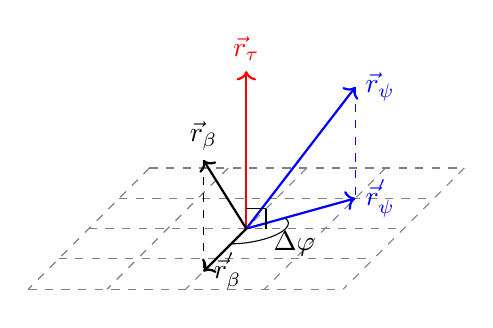
\begin{tikzpicture}
        % grid
        \draw[dashed, gray] (-2,0,-2) -- (2,0,-2);
        \draw[dashed, gray] (-2,0,-1) -- (2,0,-1);
        \draw[dashed, gray] (-2,0,0) -- (2,0,0);
        \draw[dashed, gray] (-2,0,1) -- (2,0,1);
        \draw[dashed, gray] (-2,0,2) -- (2,0,2);
        \draw[dashed, gray] (-2,0,-2) -- (-2,0,2);
        \draw[dashed, gray] (-1,0,-2) -- (-1,0,2);
        \draw[dashed, gray] (0,0,-2) -- (0,0,2);
        \draw[dashed, gray] (1,0,-2) -- (1,0,2);
        \draw[dashed, gray] (2,0,-2) -- (2,0,2);

        % vectors
        \draw[->, thick, red] (0,0,0) -- (0,2,0) node[anchor=south]{$\vec{r}_\tau$};% \tau
        \draw[->, thick, blue] (0,0,0) -- (1,1.414,-1) node[anchor=west]{$\vec{r}_\psi$};% psi
        \draw[->, thick, blue] (0,0,0) -- (1,0,-1) node[anchor=west]{$\vec{r}_\psi^{'}$};% psi_aux
        \draw[->, thick, black] (0,0,0) -- (0,1.414,1.414) node[anchor=south]{$\vec{r}_\beta$};% beta
        \draw[->, thick, black] (0,0,0) -- (0,0,1.414) node[anchor=west]{$\vec{r}_\beta^{'}$};% beta_aux

        % perp
        \draw[thin, black] (0,0.25,0) -- (0.25,0.25,0);
        \draw[thin, black] (0.25,0,0) -- (0.25,0.25,0);

        % lines
        \draw[dashed, blue] (1,1.414,-1) -- (1,0,-1);
        \draw[dashed, black] (0,1.414,1.414) -- (0,0,1.414);

        % angles
        \draw[canvas is xz plane at y=0] (0.353,-0.353) arc[start angle=-45,end angle=90,radius=0.5];

        % angles label
        \node at (0.8,0,0.5) {$\Delta\varphi$};
    \end{tikzpicture}
    \caption{}
    \label{fig:AuxLong}
\end{figure}

As shown in the Figure \ref{fig:AuxLong}, we can calculate the angle between the projections of $\vec{r}_{\psi}$ and $\vec{r}_{\beta}$ on the plane perpendicular to $\vec{r}_{\tau}$, we call these projections
\begin{equation}
    \begin{split}
        \vec{r}_{\psi}^{'}  & =\vec{r}_{\psi}-(\vec{r}_{\psi}\cdot\vec{r}_{\tau})\vec{r}_{\tau}    \\
        \vec{r}_{\beta}^{'} & =\vec{r}_{\beta}-(\vec{r}_{\beta}\cdot\vec{r}_{\tau})\vec{r}_{\tau},
    \end{split}
\end{equation}
so that we can express $\Delta\varphi$ in a simpler form
\begin{equation}
    \Delta\varphi=\arccos\frac{\vec{r}_{\psi}^{'}\cdot\vec{r}_{\beta}^{'}}{\|\vec{r}_{\psi}^{'}\|\|\vec{r}_{\beta}^{'}\|}.
\end{equation}
After some boring calculations, we can get
\begin{equation}
    \Delta\varphi=2\arccos(\sin\frac{\phi}{2}\sin\frac{\theta_{G}}{2}).
\end{equation}

After calculating each part we need, let's find the right angle $\phi$! Though section \ref{subsec:LongMainIdea}, The iterations $j=\frac{\Delta\varphi}{\omega}$ must be an integer. For equation $\Delta\varphi=j\omega$, consider both ends of the equation separately, we have
\begin{equation}
    \begin{split}
        \Delta\varphi & = 2\arccos(\sin\frac{\phi}{2}\sin\frac{\theta_{G}}{2})                            \\
                      & = 2\left(\frac{\pi}{2}-\arcsin(\sin\frac{\phi}{2}\sin\frac{\theta_{G}}{2})\right) \\
        j\omega       & = 4j\arcsin(\sin\frac{\phi}{2}\sin\frac{\theta_{G}}{2}),
    \end{split}
\end{equation}
so that we have
\begin{equation}
    \sin\frac{\phi}{2} = \frac{\sin\left(\frac{\pi}{4j+2}\right)}{\sin\frac{\theta_{G}}{2}},
\end{equation}
notice that $\phi$ has a real solution only when $\theta_{G}/2\geq\pi/(4j+2)$, may as well let $j\coloneqq\left\lceil(\pi-\theta_{G})/(2\theta_{G}) \right\rceil$, so we worked out the right angle $\phi$
\begin{equation}
    \phi\coloneqq 2\arcsin\left(\frac{\sin\left(\frac{\pi}{4j+2}\right)}{\sin\frac{\theta_{G}}{2}}\right).
\end{equation}

Let's finish with some examples of $j$ and $\phi$:
\begin{table}[h!]
    \centering
    \begin{equation*}
        \begin{array}{ccccccccccc}
            \toprule
            N        & 2   & 4 & 8        & 100      & 1000     & 10^{4}   & 10^{6}  & 10^{8}   & 10^{10}  & 2^{56} \\
            \midrule
            j        & 1   & 1 & 2        & 3        & 8        & 25       & 79      & 785      & 7854     & 78540  \\
            \phi/\pi & 0.5 & 1 & 0.677007 & 0.698709 & 0.748018 & 0.854022 & 0.90089 & 0.989752 & 0.992688 & 0.9973 \\
            \bottomrule
        \end{array}
    \end{equation*}
    \caption{}
    \label{tab:examples}
\end{table}

Can be seen as $N$ increases, the angle $\phi$ approaches $\pi$. At this point, Long's algorithm is also slightly closer to Grover's algorithm.



\section{Abdulrahman's work}

\textit{This section is based on the paper\cite{Abdulrahman_2024}, Here we restrict ourselves to the case $M=1$.}

\subsection{Main idea}

From Equation \ref{eq:IterationsGrover} we can see that when $N$ is large enough, the iterations have $R\propto 1/\theta_{G}$, so we can try to find a larger angle to reduce the number of iterations. To do this, we need a larger state space, which we might as well augment with state
\begin{equation}
    \ket{\overline{\psi}}\coloneqq H^{\otimes n}(\ket{0}^{\otimes n-1}\otimes\ket{1}),
\end{equation}
and we orthogonalize it to get the orthogonal basis $(\ket{\psi},\ket{\psi_{\perp}},\ket{\gamma})$,
\begin{equation}
    \cos\frac{\omega}{2}\ket{\gamma}\coloneqq \ket{\overline{\psi}}-\sin\frac{\omega}{2}\ket{\psi_{\perp}},
\end{equation}
which $\braket{\psi|\overline{\psi}}=0$ and $\sin(\omega/2)=\braket{\psi_{\perp}|\overline{\psi}}=\pm\sqrt{\frac{1}{N-1}}$, here the signs correspond to the $0$ and $1$ of the last bit of the search element, and we will first discuss the case where the last bit is $0$, that is, the sign is positive. In the same way, we have another orthogonal basis $(\ket{\psi},\ket{\tau},\ket{\overline{\psi}})$ which
\begin{equation}
    \sin\frac{\omega}{2}\ket{\tau}\coloneqq \ket{\psi_{\perp}}-\cos\frac{\omega}{2}\ket{\overline{\psi}}.
\end{equation}
So we have three orthogonal bases in this three-dimensional space,
\begin{equation*}
    (\ket{\overline{\psi}},\ket{\psi},\ket{\tau})
    \begin{pmatrix}
        \cos\frac{\omega}{2} & 0 & -\sin\frac{\omega}{2} \\
        0                    & 1 & 0                     \\
        \sin\frac{\omega}{2} & 0 & \cos\frac{\omega}{2}
    \end{pmatrix}
    ^{T}=(\ket{\gamma},\ket{\psi},\ket{\psi_{\perp}})
    =(\ket{\gamma},\ket{\alpha},\ket{\beta})
    \begin{pmatrix}
        1 & 0                        & 0                         \\
        0 & \cos\frac{\theta_{G}}{2} & -\sin\frac{\theta_{G}}{2} \\
        0 & \sin\frac{\theta_{G}}{2} & \cos\frac{\theta_{G}}{2}
    \end{pmatrix}
    .
\end{equation*}
\begin{figure}[h]
    \centering
    \begin{subfigure}[b]{0.33\columnwidth}
        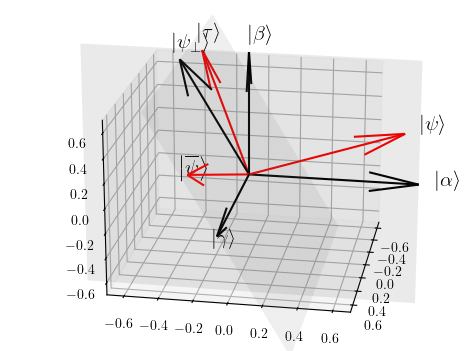
\includegraphics[width=\columnwidth]{figures/basic_3.png}
        \caption{orthogonal basis $(\ket{\overline{\psi}},\ket{\psi},\ket{\tau})$}
    \end{subfigure}
    \begin{subfigure}[b]{0.33\columnwidth}
        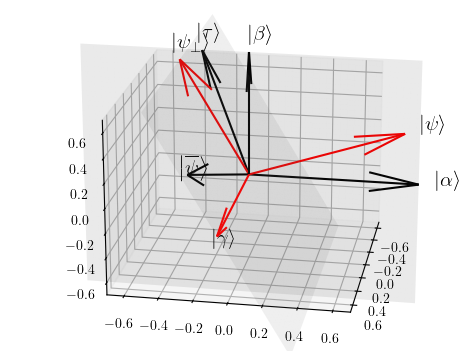
\includegraphics[width=\columnwidth]{figures/basic_2.png}
        \caption{orthogonal basis $(\ket{\gamma},\ket{\psi},\ket{\psi_{\perp}})$}
    \end{subfigure}
    \begin{subfigure}[b]{0.33\columnwidth}
        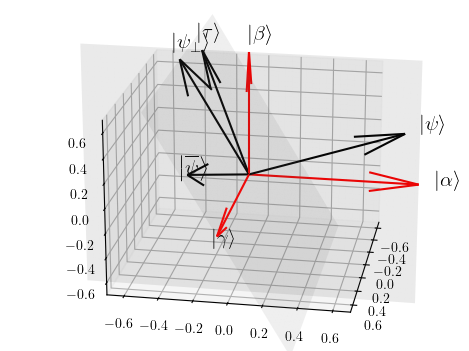
\includegraphics[width=\columnwidth]{figures/basic_1.png}
        \caption{orthogonal basis $(\ket{\gamma},\ket{\alpha},\ket{\beta})$}
    \end{subfigure}
    \caption{Three orthogonal bases}
    \label{fig:basics}
\end{figure}

After a basic understanding of this space, we can start to make some improvements. We require a rotation that is independent of the target element, considering the rotation in the space spanned by $\ket{\psi}$ and $\ket{\overline{\psi}}$, in the sub-space $(\ket{\overline{\psi}},\ket{\psi},\ket{\tau})$ we can write this rotation as
\begin{equation}
    A(\phi)\coloneqq H^{\otimes n}X^{\otimes n}c^{n-1}\left(R_{y}(\phi)\right)X^{\otimes n}H^{\otimes n}=
    \begin{pmatrix}
        \cos\frac{\phi}{2} & -\sin\frac{\phi}{2} & 0 \\
        \sin\frac{\phi}{2} & \cos\frac{\phi}{2}  & 0 \\
        0                  & 0                   & 1
    \end{pmatrix}
    .
\end{equation}
Our objective is to maximize the probability of finding the target element, notice that
\begin{theorem}
    Considering vectors $\vec{m},\vec{n}\in\mathbb{R}^{3}$ and angle $\phi\in[0,2\pi]$, for a certainly axis defined by vector $\vec{l}$, the inner product $\vec{m}\cdot\left(\exp\left(\phi\vec{l}\cdot\vec{J}\right)\vec{n}\right)$ take the extreme only when $\mathrm{rank}\left(\left(\vec{m},\vec{n},\vec{l}\right)\right)<3$, which $J_{j}$ are the three generators of Lie group $SO(3)$.
\end{theorem}
According to this theorem, we can see that the maximum probability is achieved when the state after the rotation is in the plane spanned by $\ket{\gamma}$ and $\ket{\beta}$. So we just need angles $\phi$ such that $A(\phi)$ keeps the states after each iteration in the plane spanned by $\ket{\gamma}$ and $\ket{\beta}$, we extend the Grover iteration $G=DO$ to
\begin{equation}
    Q=A(\phi)G=A(\phi)DO.
\end{equation}



\subsection{Keep states in the plane}

For convenience, we use basis $(\ket{\overline{\psi}},\ket{\psi},\ket{\tau})$ and spherical coordinates $(x,y,z)^{T}\to(\sin\frac{\theta}{2}\sin\varphi,\sin\frac{\theta}{2}\cos\varphi,\cos\frac{\theta}{2})^{T}$ to describe this space. After some calculations, we have
\begin{equation}
    \ket{\beta}=(\sin\frac{\theta_{\beta}}{2}\sin\frac{\pi}{4},\sin\frac{\theta_{\beta}}{2}\cos\frac{\pi}{4},\cos\frac{\theta_{\beta}}{2})^{T},
\end{equation}
where $\sin(\theta_{\beta}/2)=\sqrt{2/N}$, so the space spanned by $\ket{\gamma}$ and $\ket{\beta}$ can be write as $\varphi=\pi/4$. We need to get the initial state into the plane first, so we apply $A_{0}\coloneqq A(-2(\varphi_{\beta}-\varphi_{\psi}))=A(-\pi/2)$ to $\ket{\psi}$ so that
\begin{equation}
    A_{0}\ket{\psi}=(\sin\frac{\pi}{4},\cos\frac{\pi}{4},0)^{T}.
\end{equation}
Next, let's consider the effect of the Grover iteration $G$ on the angle $\varphi$, what can be computed is that the Oracle gives us the mapping
\begin{equation}
    \begin{split}
        O\colon & \frac{\theta}{2}\to\pi-\frac{\theta}{2}+\theta_{\beta} \\
                & \varphi\to\varphi
    \end{split}
\end{equation}
and the diffusion operation gives us the mapping
\begin{equation}
    \begin{split}
        D\colon & \frac{\theta}{2}\to\pi-\frac{\theta}{2} \\
                & \varphi\to-\varphi.
    \end{split}
\end{equation}
Since the plane gives us the angle $\varphi=\pi/4$, we need to operate $A\coloneqq A(-2(\varphi-(-\varphi)))=A(-\pi)$ to pull back the angle $\varphi$ to $\pi/4$, so the operation $Q$ gives us the mapping
\begin{equation}
    \begin{split}
        Q=AG\colon & \frac{\theta}{2}\to\frac{\theta}{2}-\theta_{\beta} \\
                   & \varphi\to\varphi.
    \end{split}
\end{equation}
Can be seen that operation $Q$ keeps the state in the plane spanned by $\ket{\gamma}$ and $\ket{\beta}$, so we visualize this plane to further observe the role of operation $Q$, with $\sqrt{1-\bra{\beta}A_{0}\ket{\psi}^{2}}\ket{\beta_{\perp}}=A_{0}\ket{\psi}-\ket{\beta}\bra{\beta}A_{0}\ket{\psi}$.
\begin{figure}[h]
    \centering
    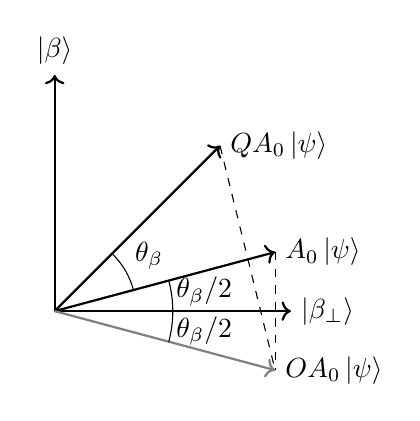
\begin{tikzpicture}
        % 绘制箭头
        \draw[->, thick] (0,0) -- (0,3) node[anchor=south] {$\ket{\beta}$};
        \draw[->, thick] (0,0) -- (2.1,2.1) node[anchor=west] {$QA_{0}\ket{\psi}$};
        \draw[->, thick] (0,0) -- (2.8,0.75) node[anchor=west] {$A_{0}\ket{\psi}$};
        \draw[->, thick] (0,0) -- (3,0) node[anchor=west] {$\ket{\beta_{\perp}}$};
        \draw[->, gray, thick] (0,0) -- (2.8,-0.75) node[anchor=west,black] {$OA_{0}\ket{\psi}$};
        % 绘制虚线
        \draw[dashed] (2.8,0.75) -- (2.8,-0.75);
        \draw[dashed] (2.1,2.1) -- (2.8,-0.75);
        % 绘制角度标记
        \draw (1.5,0) arc[start angle=0,end angle=15,radius=1.5];
        \draw (1.5,0) arc[start angle=0,end angle=-15,radius=1.5];
        \draw (1,0.27) arc[start angle=15,end angle=45,radius=1];
        % 标记角度
        \node at (1.9,0.25) {$\theta_{\beta}/2$};
        \node at (1.9,-0.25) {$\theta_{\beta}/2$};
        \node at (1.2,0.7) {$\theta_{\beta}$};
    \end{tikzpicture}
    \caption{}
    \label{fig:Abdulrahman}
\end{figure}

As shown in the Figure \ref{fig:Abdulrahman}, we can see that the operation $Q=ADO$ gives us a rotation of angle $\theta_{\beta}$, So we just need applying $R_{Q}=\left\lfloor\frac{\pi-\theta_{\beta}/2}{\theta_{\beta}}\right\rceil$ times operation $Q$ on $A_{0}\ket{\psi}$ to approximate $\ket{\beta}$, when the number of searches $N$ is large enough,
\begin{equation}
    Q^{R_{Q}}A_{0}\ket{\psi}=\cos(\frac{2R_{Q}+1}{2}\theta_{\beta})\ket{\beta_{\perp}}+\sin(\frac{2R_{Q}+1}{2}\theta_{_{\beta}})\ket{\beta}\approx\ket{\beta},
\end{equation}
we have the ratio of the number of iterations after and before refinement $R_{Q}/R\approx\theta_{G}/\theta_{\beta}\approx 1/\sqrt{2}$.

It seems that this violates the lower bound on the number of iterations we computed in section \ref{sec:BoundForGrover}, but we did restrict the search element. If the last bit of the search element is $1$, what can be calculated is $A_{0}=A(\pi/2)$ and $A=A(\pi)$, such that we need to distinguish the last digit of the search element first, so we're essentially trading one bit of state space for this $\sqrt{2}$ speedup.


%-----------------------bib---------------------------

\bibliographystyle{plain}
\bibliography{ref}


\end{document}